
%-----------------------------------------------------------------------------
%	CONTENT STRUCTURE
%-----------------------------------------------------------------------------


\chapter{Introduction: Imbalanced Classification Learning}

%\setlength{\epigraphwidth}{3.5in} 
%\epigraph{\textit{``Most people do not listen with the intent to understand; they listen with the intent to reply."} --- Stephen R Covey}

%Artificial intelligence (AI), powered by machine learning (ML), is transforming the world we live in today. 
%AI and ML applications which were previously limited to constrained environments are nowadays widely deployed in almost every field in the wild. 
%ML techniques are broadly classified intro two categories based on the nature of output random variable.
%Firstly, classification models deal with discreet random variables and hence model categorical distributions. 
%Lastly, regression models deal with continuous random variables hence model continuous distributions.
Machine learning (ML) based classifiers have numerous applications in real world; e.g., spam email detection, cancerous tumor detection, fraudul transaction detection, text sentiment analysis and emotion analysis, image classification and object detection, named entity recognition and information extraction.
Classifiers are usually studied under balanced categorical distributions (BCD) for simplicity; many datasets curated and used by academia have balanced categories. %\footnote{Many text classification datasets made accessible via huggingface-datasets, tensorflow-datasets and torchtext are purposefully balanced: e.g. even though DBpedia ontology classes are imbalanced in nature, the commonly used DBpedia-14 dataset is balanced.},
%e.g., SNLI \cite{maccartney-manning-2008-snli}, Sentiment Classification (IMDb reviews) \cite{maas-etal-2011-imdbreview}, MultiNLI \cite{williams-etal-2018-multinli}, XNLI \cite{conneau-etal-2018-xnli}, CIFAR-\{10,100\} \cite{Krizhevsky-2009-CIFAR}, nearly balanced, e.g. MNIST \cite{lecun1998-mnist}.
However, naturally occurring categorical distributions are often imbalanced. 
In many real-world settings, imbalance is inevitable, e.g. fewer cancerous patients than non-cancerous, fewer fraud transactions than legit, spam and ham mails are not evenly distributed.
And in some scenarios balancing is impossible; e.g. image segmentation task has more background pixels than the foreground pixels, and in natural languages, the each stopword type has more tokens than each content type.
An imbalanced categorical distribution (ICD) results in the formation of majority and minority categories.\footnote{
The terms \textit{majority} and \textit{minority} may sometimes be referred as \textit{frequent} and \textit{rare}, respectively. The term \textit{category} is referred as \textit{class} in the context of machine learning, as \textit{group} in social sciences, \textit{symbol} in symbolic communication systems, and as \textit{type} in the context of natural language processing.} 
The minority categories are at least as important, if not more, as majority categories. 

When ML classification techniques are applied on imbalanced distributions without accounting for the imbalance, we face the following two problems:
\begin{enumerate}
\item There exist noticeable performance difference between majority and minority classes. 
% The difference varies based on the level of imbalance. 
Classifiers achieve higher performance (usually quantified using F-measure) on the majority classes whereas relatively poor performance on minority classes. 
Sometimes this phenomenon is attributed as frequency-based biases; specifically, minority classes suffer from under-recall, hence poor recall, and the majority classes suffer from over-recall, hence poor precision.

\item Evaluation metrics that do not consider imbalance into account, e.g, Accuracy, overlook performance on minority categories. 
Rounding the system level score to a few decimal points is a common practice which helps masking out unnecessary detail and establishing significance in the performance improvements. 
When majorities and minorities are put together without addressing the imbalance and rounded the resulting system level score to a few decimal points, the impact of minorities performance looks too small that they risk being \textit{ignored} or \textit{not significant}.
\end{enumerate}


The problem of imbalance in categorical distributions is studied in classical ML era \cite{provost2000-ml-imb-101, japkowicz2002ClassImbalance,chawla-etal-2004-special-issue}.
In the medical domain \citet{Maciej2008MedicalImbalance} find that classifier performance deteriorates with even modest imbalance in the training data.
However, with the neural networks, there is only scant effort:
Untreated class imbalance has been known to deteriorate the performance of image segmentation; 
\citet{Sudre2017GeneralizedDice} investigate the sensitivity of various loss functions.
\citet{buda-etal-2018-imbalance-cnn} investigate the impact of class imbalance on convolutional neural networks' classification performance and also conclude that class imbalance is detrimental. % definition and quantification method for two types of class imbalance: \textit{step imbalance} and \textit{linear imbalance}.
%Since the imbalance in Zipfian distribution of classes is neither single-stepped nor linear, we use a divergence based measure to quantify the imbalance.


%\textcolor{gray6}{
Though the imbalanced categorical distributions are prevalent in almost every domain, the efforts towards learning from imbalanced distributions is mostly targeted to computer vision tasks \cite{Johnson2019SurveyImbalance}.
With neural network being a universal function approximator and deeplearning becoming mainstream machine learning paradigm, the boundaries between different kinds of tasks are favorably blurred: the deeplearning models are borrowed from one domain to other: CNN models which were originally used for computer vision are now being used for natural language processing (NLP), and the Transformer models which were originally used for NLP tasks are now also being used for computer vision.
Hence, we believe the findings on imbalanced learning can also be transferrable from one domain to the other, although it is not formally verified before.

In this work, we like to take the learning from tasks where imbalanced learning is well explored and apply it to the areas such as natural language generation where the efforts are scant.
It is known that word types in natural languages resemble Zipfian distribution \cite{zipf1949human,powers-1998-zipf-apps}, which is an extremely imbalanced, long-tail distribution. 
In any natural language system, some word types occur very frequently and a vast number of types occur rarely. 
In a typical class imbalanced setting, ML models tends to have high performance on majority classes, as there are plenty of examples to learn from, while poor performance on minority classes for which there are only a limited number of examples.
In symbolic communication systems, the rare \textit{symbols} contain more \textit{information content} than frequent symbols \cite{shannon1948mathematical}.
Since natural languages are also symbolic communication systems, rare types are equally or more important than the frequent types \cite{gowda2021macroaverage}. 
The imbalance problem in language systems is particularly challenging and requires our attention due to the fact that rare types carry crucial information \cite{steedman-2008-last}.
For example, machine translation models trained have poor performance for the rare types where the crucial information is \cite{gowda-may-2020-finding,gowda2021-many-eng}.
Hence, we emphasize that extra care concerning the imbalance is necessary for the application of ML to natural language processing (NLP), and we attempt to address exactly that in this work.

We present our findings in the following order:
In Chapter \ref{ch:affirmative-action}, we describe that the objective of imbalance learning is \textit{going the extra mile} in favor of minority categories, whose parallel counterpart in the social sciences is called \textit{affirmative action} (AA), and discuss its ethical implications. 
In Chapter \ref{ch:nlg-imbalance}, we focus on (neural) machine translation (NMT), a natural language generation task and show the consequences of imbalance.
NMT is commonly not seen as classification task and class imbalance is ignored, we envision NMT model as a kind of multi-class classification task where classes are the target language vocabulary, we show that imbalance affects hyperparamaters such as vocabulary size and show that NMT models have biases resulting from class imbalance which was previously unknown.
In Chapter \ref{ch:eval-metrics}, we show that current evaluation metrics are ignorant of imbalance, and some new ones proposed are biased and opaque; we present an evaluation metric that accounts class imbalance at the testing stage.
In Chapter \ref{ch:imb-learning}, we study both the methods and our proposed methods for machine learning from imbalanced categorical distributions.
Here we consider NMT as a complex classification task, we start with simple classification tasks such as image classification, text classification and build our way to the NMT task.
In Chapter \ref{ch:applications}, by applying our simplified view of NMT as multi-classifier on the target language, we develop many-to-one translation model. While current multilingual NMT efforts are limited to 100 languages, we push its limits with 500 to English translation (i.e. 4 times more source languages). 


\begin{figure}[ht]
    \centering
    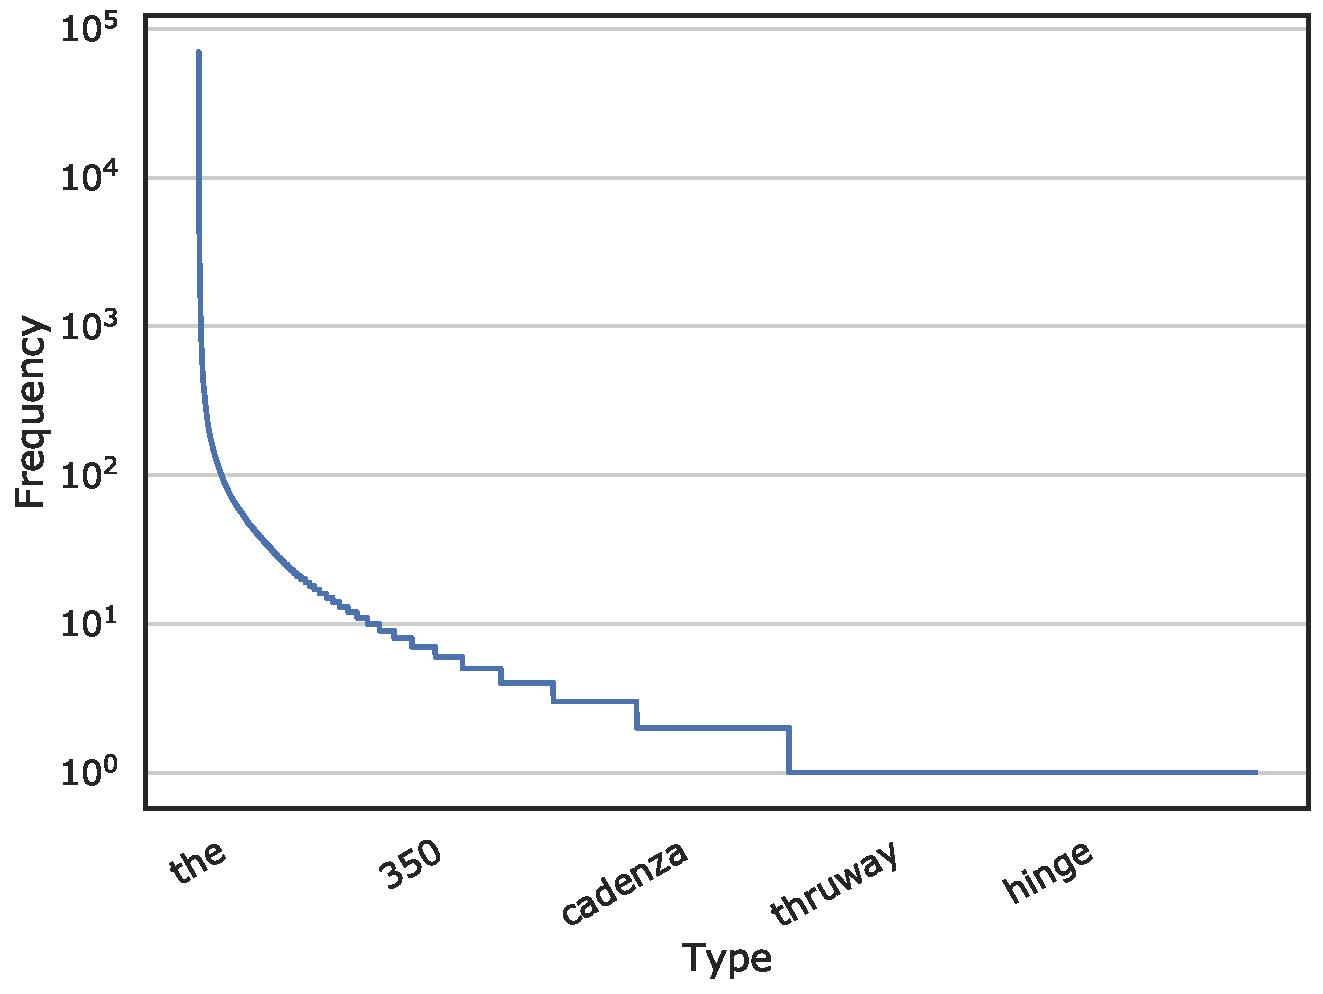
\includegraphics[width=0.75\textwidth]{img/background/brown-corpus-zipf.pdf}
    
    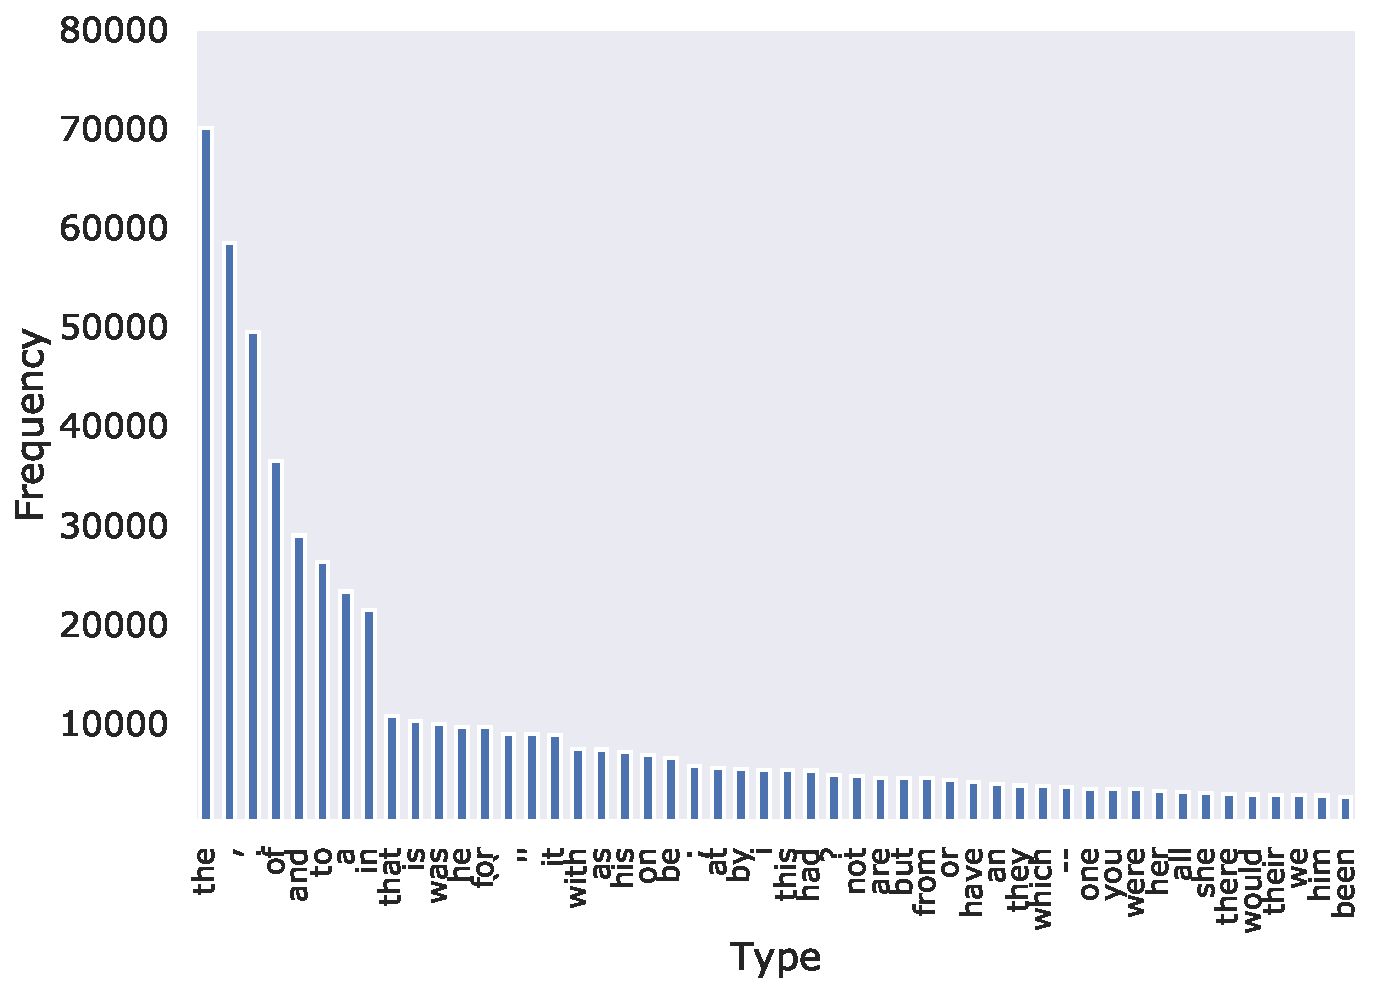
\includegraphics[width=0.75\textwidth]{img/background/brown-corpus-zipf-top50.pdf}
    \caption{Caption}
    \label{fig:my_label}
\end{figure}
\begin{figure}[ht]
    \centering
    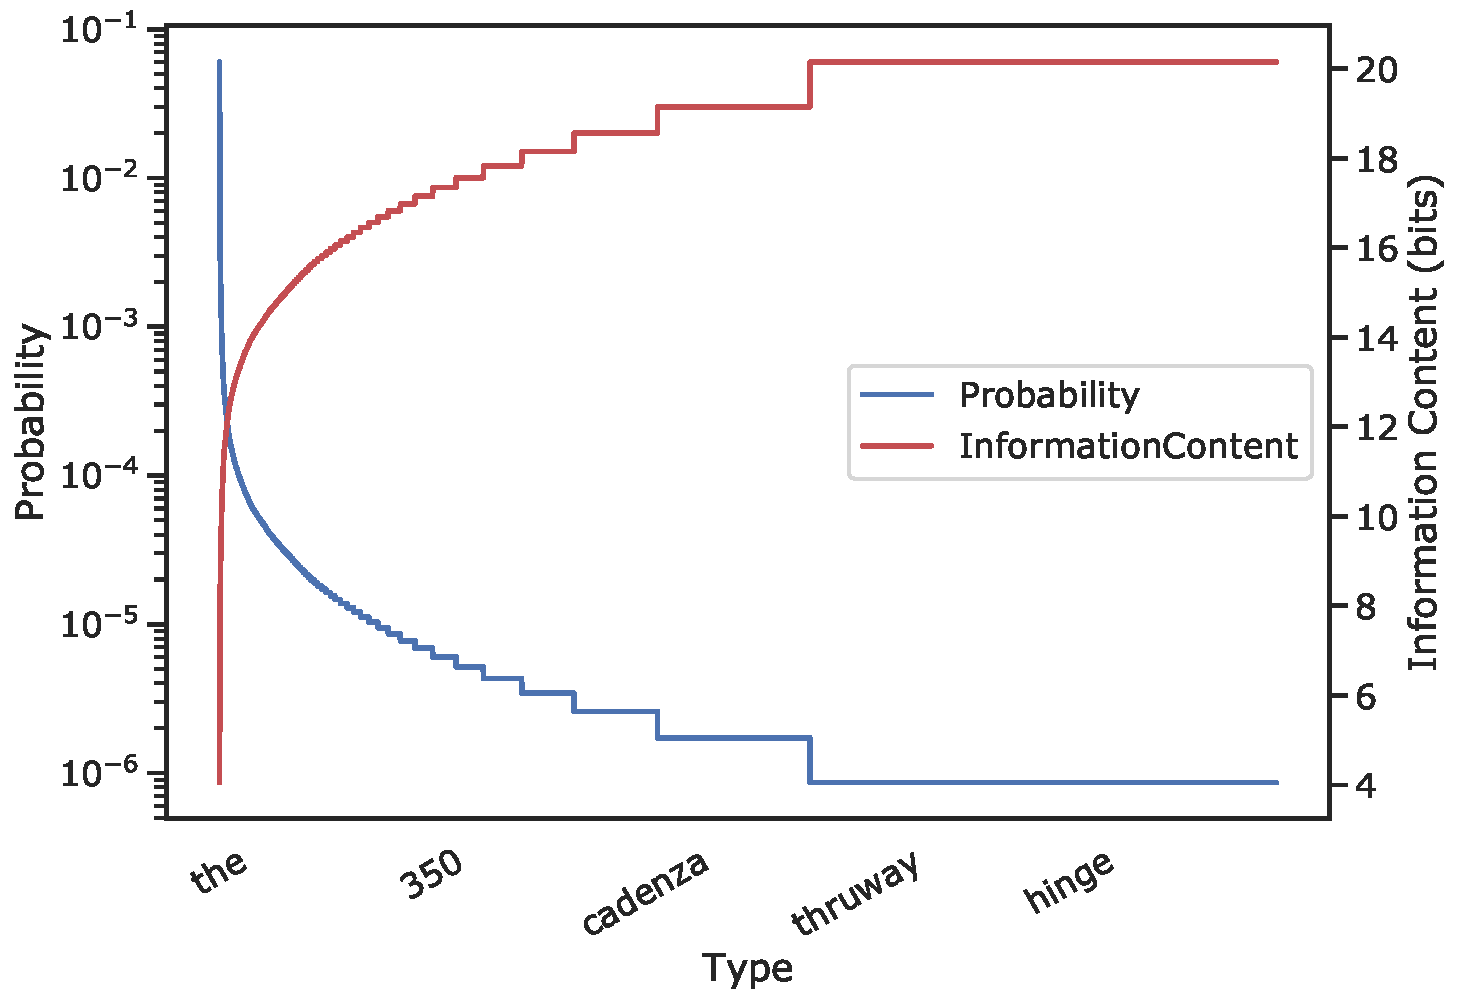
\includegraphics[width=0.75\textwidth, trim={3mm 0 3mm 0}, clip] {img/background/brown-corpus-shannons.pdf}
    \caption{Caption}
    \label{fig:my_label}
\end{figure}


%%---- COMMENT -----
\begin{comment}
Consider rare type translation: when the source and the target languages use the same alphabet,
%e.g. Romance languages such as English, French, Spanish, German, etc,
the rare types such as proper nouns and numeric types are often cognates which can be simply copied from the source to the target side without translation or transliteration. 
Shared vocabulary with tied embeddings which is widely used in the current translation models exploit this phenomenon ~\cite{press-wolf-2017-embeddings,vaswani2017attention}.
However, when translating between languages of heterogeneous scripts, rare word translation is more problematic.
Though techniques such as byte-pair-encoding \cite{sennrich-etal-2016-bpe} alleviate this problem, it is not entirely resolved ~\cite{gowda-may-2020-finding}.

\begin{figure}
    \centering
    \includegraphics[width=\linewidth]{img/gtranslate-error2.png}
    \caption{An example error from Google Translate {\footnotesize (accessed: June 15, 2021)}: `984' (in Kannada script) is translated to `2' in English; `984' is the crucial information in this example sentence.}
    \label{fig:gtrans-err}
\end{figure}
\end{comment}

%%---- COMMENT -----

\textbf{Proposal:} We propose to study and advance the following research arenas:
\begin{enumerate}
 \item How is class imbalance affecting NLG?
 \item Are the current NLG evaluation metrics addressing class imbalance? If not, how to create a metric that address imbalance?
 \item How to improve NLG performance in the light of imbalance?
\end{enumerate}

%We aim to study imbalanced learning under the realm of neural machine translation (NMT) task, however, since classifier is entangled with an autoregressor in NMT, certain imbalance learning strategies such as over-sampling and under-sampling are not directly applicable. 
%Imbalanced learning is widely studied under clearly defined classification tasks such as image classification. 

\chapter{Background: Machine Translation}
\label{ch:ml-background}

Machine translation (MT) is the problem of translating text from one natural language to another using machine learning (ML) methods. 
An ML problem can be precisely defined as the problem of improving some measure of performance when executing some task, through some type of training experience~\cite{mitchell2017key}.
The MT problem typically involves learning from a set of human translated text (also called \textit{parallel data}, or \text{bitext}) with the goal of producing human-like translations on unseen data.
MT has been studied since the 1950s \cite{reifler1954first-cmt}, and more actively since the 1990s \cite{brown-etal-1988-statistical,brown-etal-1993-mathematics,knight1999statMT-tutorial}\footnote{\url{https://web.archive.org/web/20170310234937/https://www.statmt.org/survey}}.
Currently, neural machine translation (NMT) \cite{sutskever2014seq2seq,vaswani-2017-attention} is the dominant MT paradigm, which is described in the following.



\section{Neural Machine Translation}

%MT is the problem of translating text from one natural language to another.
Formally, MT is a sequence-to-sequence transduction task, i.e, a task of transforming sequences of form $x_{1:m} = x_1 x_2 x_3 ... x_m$ to the form $y_{1:n} = y_1 y_2 y_3 ... y_n$, where $x_{1:m}$ is in source language $X$ and $y_{1:n}$ is in target language $Y$. 
Each item in the sequence is a discrete token, i.e., $\forall x_i \in V_X $ and $\forall y_j \in V_Y$,  where $V_X$ and $V_Y$ are vocabularies of $X$ and $Y$ languages, respectively.

%\subsection{Neural Machine Translation}

NMT uses artificial neural networks to achieve translation. 
Historically, MT pipelines involved a set of independently optimized components such as parsers, word aligners, and language models.
NMT simplifies the pipeline by enabling end-to-end optimization of all parameters to achieve the translation objective. 
Even though there are many variations of NMT architectures, all share the common objective of:

$$\hat\theta = \argmax_{\theta \in \Theta} \prod_{(x_{1:m}, y_{1:n}) \in \mathcal{D}} P(y_{1:n} | x_{1:m}; \theta)$$

where $\theta$ is the set of all parameters, and $\mathcal{D}$ is a set of parallel sentences.
For most cases, the above objective function is decomposed autoregressively as
% \footnote{There are only a few models that perform non-autoregressive NMT \cite{libovicky-helcl-2018-end,Gu-etal-17-NonAR-NMT}. These are focused on improving the speed of inference; generation quality is currently sub-par compared to autoregressive models.} 
$$\hat\theta = \argmax_{\theta \in \Theta} \prod_{(x_{1:m}, y_{1:n}) \in \mathcal{D}} \prod_{t=1}^{n} P(y_t | y_{<t}, x_{1:m}; \theta)$$ 

Maximization of likelihood is equivalent to minimization of negative $\log$ likelihood:

$$\hat\theta = - \argmin_{\theta \in \Theta} \sum_{(x_{1:m}, y_{1:n}) \in \mathcal{D}} \sum_{t=1}^{n} \log P(y_t | y_{<t}, x_{1:m}; \theta)$$

In practice,
$$\hat\theta = - \argmin_{\theta \in \Theta} \mathop{\mathbb{E}}_{(x_{1:m}, y_{1:n}) \in \mathcal{D}} \frac{1}{n} \sum_{t=1}^{n} \log P(y_t | y_{<t}, x_{1:m}; \theta)$$


The discriminator function is commonly implemented as a pair of \textsc{Encoder-Decoder} networks.
Formally,
$$ P(y_t | y_{<t}, x_{1:m}) = \textsc{Decoder}(y_{<t}, \textsc{Encoder}(x_{1:m}; \phi); \psi)$$
%$$ P(y_t | y_{<t}, x_{1:m}) = P(y_{<t} | a_t)$$
Multiple implementations for \textsc{Encoder} and \textsc{Decoder} are available: recurrent neural networks (RNN) such as Long Short-Term Memory \cite{sutskever2014seq2seq,hochreiter1997LSTM} and Gated Recurrent Unit \cite{cho-etal-2014-properties,cho2014learning}, RNN with attention \cite{bahdanau2014nmtattn,luong2015effectiveAttn}, convolutional neural networks (CNN) \cite{gehring2017CNNMT} and Transformer \cite{vaswani-2017-attention}. 
 We use Transformer for all our NMT experiments in the later chapters as it is the current best performing model.
 We refer to \citet{rush-2018-annotated} for the implementation details of Transformer.

At the inference time, the model's hypothesis sequence is generated in a loop, with $h_0=\code{<s>}$, a special token denoting the \textit{beginning-of-sequence}, until  $h_t=\code{[/s]}$, denoting the \textit{end-of-sequence}. Both \code{<s>} and \code{</s>} are special types added to vocabulary $V_Y$. Similarly, during the training time, the sequence $y_{1:n}$ has a prefix, $y_0=\code{<s>}$, and suffix, $y_{n+1}=\code{</s>}$, to resemble the inference time conditions.

At each time step $t$ during inference, the hypothesis token is predicted as, 
$$ h_t = \argmax_{c \in V_Y} P(c | h_{<t}, x_{1:m}) \text{, for } t=1, 2,  ... \text{ until } h_t = \code{</s>}$$

The above greedy decision of choosing local maximum at each time step may lead to search errors.
We use beam search to further improve the overall sequence generation quality.

\section{Evaluation}
\label{ch:background-sec:eval}

Evaluation of ML models is essential to keep track of progress made on a task, to separate good ideas from the bad, and also to determine the best one among several competing choices. 
Manual evaluation, although desired, is often slow, expensive, and infeasible.
Hence, automatic evaluation metrics are used whenever possible. 
The choice of evaluation metric varies from task to task. 
The following sections describe common metrics used in classification and machine translation tasks. 

\textbf{Notation:} consider a set of $C = \{ 1, 2, .. K \}$ classes, and a held-out set, $T = \{ (x^{(i)}, y^{(i)}, h^{(i)}) | i = 1, 2, 3, ... N \}$, where $x^{(i)}$ is the input, $y^{(i)} \in C$ is the ground truth (i.e., gold labels) and $h^{(i)} \in C$ is a prediction from an ML model (also known as the hypothesis). 
Let $\ind{y^{(i)}, h^{(i)}}$ be an indicator function with unity value when arguments match, and zero otherwise.
For notational simplicity, let $\ind{y^{(i)}, h^{(i)}, c} = \ind{y^{(i)}, h^{(i)}} \times \ind{h^{(i)}, c}.$


\subsection{Classifier Evaluation}
\label{ch:background-sec:cls-eval}
Accuracy is one of the most simple and widely used evaluation metrics, which is computed as:
% $$Accuracy=\frac{Correct}{Total}$$

$$Accuracy = \frac{\sum_i^N \ind{y^{(i)}, h^{(i)}}}{N}$$

Accuracy provides an overall system performance by treating each \textit{instance} equally. For a fine-grained performance report, we compute Precision ($P_c$) and Recall ($R_c$) measures separately for each class type ($c$) as: 

$$P_c = \frac{\sum_i^N \ind{y^{(i)}, h^{(i)}, c}} {\sum_j^N \ind{h^{(j)}, c}}$$
$$R_c = \frac{\sum_i^N \ind{y^{(i)}, h^{(i)}, c}} {\sum_j^N \ind{y^{(j)}, c}}$$

F-measure combines both precision and recall metrics using harmonic mean, as:
$$F_{\beta;c} = \frac{(1+\beta^2) \times P_c \times R_c}{(\beta^2 \times P_c) + R_c}$$

where parameter $\beta$ controls the relative importance of precision and recall.
While in most applications, precision and recall are equally important (i.e., $\beta=1$), in certain scenarios, recall may be more important than precision (or vice versa). For example, $\beta=2$ implies that recall is twice as important as precision.

The overall performance of a classification system is obtained by taking an average of performance across all classes.

$$WeightedF_\beta = \frac{\sum_{c=1}^K w_c \times F_{\beta;c}}{ \sum_{j=1}^K w_j}$$
where $w_c$ is the weight assigned to class. 
If the held-out dataset has balanced classes, i.e., all classes have approximately the same number of instances, the methodology used to average across classes is uninteresting.\footnote{The research community has avoided dealing with class imbalance by using balanced held-out sets; e.g., SNLI \cite{maccartney-manning-2008-snli}, CIFAR-\{10,100\} \cite{Krizhevsky-2009-CIFAR}, sentiment classification of IMDb reviews \cite{maas-etal-2011-imdbreview}, MultiNLI \cite{williams-etal-2018-multinli}, XNLI \cite{conneau-etal-2018-xnli}.} 

However, in the imbalanced classes scenarios, the averaging methodology requires careful consideration. There are two schools of thought about choice for $w_c$:

\begin{itemize}
\item \textbf{Micro-averaging:} Treats each \textit{instance equally}, i.e., $w_c = freq(c) = \sum_{i=1}^N \ind{y^{(i)}, c}$. 
In this method, classes with more instances (i.e., majority classes) have a huge impact on system performance compared to classes with fewer instances (i.e., minority classes).

\begin{equation}\label{eq:microf}
  MicroF_\beta = \frac{\sum_{c=1}^K freq(c) \times F_{\beta;c}}{N}  
\end{equation}

%where $freq(c)$ is the frequency of c in ground truth, i.e., $freq(c) = \sum_{i=1}^N \ind{y^{(i)}, c}$
In problems having exactly one label per instance (i.e., not multi-label classification), both micro-precision ($MicroP$) and micro-recall ($MicroP$) are equal to \textit{accuracy}, which is equivalent to $MicroF$. 
Therefore, all these micro metrics can be efficiently calculated as,
\begin{equation}\label{eq:microf-simple}
   MicroP = MicroR = MicroF = \frac{\sum_i^N \ind{y^{(i)}, h^{(i)}}}{N} 
\end{equation}

\item \textbf{Macro-averaging}: Treats each \textit{class} equally, i.e., $w_c=1, \forall c \in C$. 
\begin{equation}\label{eq:macrof}
  MacroF_\beta = \frac{\sum_{c=1}^K F_{\beta;c}}{K}  
\end{equation}


In this method, all \textit{classes} have equal contribution to system performance. 
As a result, in imbalanced class datasets, minority class \textit{instances} have higher weights than majority class instances. 
\end{itemize}


\subsection{Machine Translation Evaluation: BLEU}

\textbf{BLEU} \cite{papineni-etal-2002-bleu} is the most popular evaluation metric for machine translation, formulated as the geometric mean of n-gram precision ($P_n$), up to 4-grams. 
  $$ BLEU = BP \times \Big(\prod_{n=1}^4 P_n \Big)^\frac{1}{4}$$
where, BP is brevity penalty, intended to penalize shorter translations resulting from poor recall.

$$ BP = \exp(\min\{1-\frac{R}{H},\space 0\}) $$ 
where, $R$ and $H$ are lengths (i.e., number of tokens) of reference and hypothesis, respectively.
 
To compute n-gram precision, $P_n$, we need the following utilities: 

%Consider a test corpus, $T = \{ (x^{(i)}, h^{(i)}, y^{(i)}) | i = 1,2,3...m \}$ where $x^{(i)}$, $h^{(i)}$, and $y^{(i)}$ are source, system hypothesis, and reference translation, respectively. Let $x = \{x^{(i)} \forall i\}$ and similar for $h$ and $y$. 
Let $\textsc{Ngram}(n, a)$ return the set of all n-gram types in sequence $a$, 
 
 %$$\textsc{Ngram}(n,a) = \{ a_i a_{i+1} ... a_{i+n-1}\}_{i \in [1, 2, ... (|a|+1-n)]}$$
 $$\textsc{Ngram}(n,a) = \{ a_{i:i+n} \}_{i \in [1, 2, ... (|a|+1-n)]}$$
 
where, $|a|$ is the length of sequence $a$ (i.e., number of tokens). Let $\textsc{Ngrams}(n)$ return all n-grams from all hypotheses,
$$\textsc{Ngrams}(n) = \bigcup_{i=1}^N \textsc{Ngram}(n, h^{(i)})$$
Finally, the combined precision for n-grams of size $n \in [1, 4]$, 
\begin{equation}\label{eq:bleu-precision}
  P_n = \frac{\sum_{c \in \textsc{Ngrams}(n)} \textsc{freq}(c) \cdot P_c} {\sum_{c' \in \textsc{Ngrams}(n)} \textsc{freq}(c')} 
\end{equation}
where $P_c$ is precision of n-gram type $c$, and $\textsc{freq}(c)$ is frequency of $c$ in \textit{hypotheses}.

As mentioned in Section~\ref{ch:background-sec:cls-eval}, there exist an efficient method for calculating micro metrics which does not keep track of performance per each class type (see Equations \ref{eq:microf} and \ref{eq:microf-simple}). 
Similarly, $P_n$ can also be efficiently calculated as following:
\begin{equation}\label{eq:bleu-precision-simple}
P_n = \frac{\sum_i^N \sum_{{c} \in \textsc{Ngram}(n, h^{(i)})}  \min\{\textsc{Count}(c, h^{(i)}), \textsc{Count}(c, y^{(i)}) \}}{ \sum_j^N (|h^{(j)}| + 1 - n)}     
\end{equation}
where $\textsc{Count}(c, a)$ return the total times n-gram type $c$ occur in sequence $a$.

We highlight two shortcomings of \bleu{} regarding rare phenomena learning:
\begin{enumerate}
    \item As per our categorization of metrics in Section \ref{ch:background-sec:cls-eval}, BLEU is a \text{micro} metric, as it treats each n-gram instance equally. 

    \item \bleu{} implementations provide $P_n$, which is the combined precision of all grams of length $n$, and do not provide performance breakdown for each n-gram type. For instance, \bleu{} provides $P_1$ which is the combined precision of all unigrams, but not precision of a specific type, such as $P_{the}$. 
    Similarly, \bleu{} does not provide recall measure for types. Precision and recall measures for each class type is important to recognize performance difference between frequent and rare types.
\end{enumerate}

We address these two shortcomings in a later chapter.

\begin{comment}
$\forall \textsl{g} \in \textsc{Ngram}(n, a)$, let $\textsc{Count}(g, a)$ returns total instances of n-gram type in $a$.

$$\textsc{Count}(g, a) = \sum_{t=1}^{|a| - |g|} \ind{g, a_{t:t+|g|}}$$

Let $\textsc{Match}(\textsl{g}, a, b)$ returns the number of times n-gram instances of type $\textsl{g}$ \textit{matched} between a pair of sequences, $a$ and $b$.

$$\textsc{Match}(\textsl{g}, a, b) = \sum_{i=1}^m \min\{\textsc{Count}(\textsl{g}, a), \textsc{Count}(\textsl{g}, b)\}$$

Finally, the precision for all $n$-grams, where $n \in \{1,2,3,4\}$, is given by,
$$
P_n = \frac{\sum_i^N \sum_{{g} \in h^{(i)}} \textsc{Match}(\textsl{g}, h^{(i)}, y^{(i)})}
{ \sum_j^N (|h^{(j)}| + 1 - n)} 
$$

%We will use the above notations metrics with the same in Chapter~\ref{ch:eval-metrics}. 

We highlight two shortcomings of \bleu{} regarding rare phenomena learning, which we address in a later chapter:
\begin{enumerate}
    \item As per our categorization of metrics in Section \ref{ch:background-sec:cls-eval}, BLEU is a \text{micro} metric, as it treats each n-gram instance equally. 

    \item $P_n$ is the combined precision of all grams of length $n$, and there is no performance breakdown for each type of n-gram. For instance, \bleu{} provides $P_1$ which is the combined precision of all unigrams, but not precision of a specific type, such as $P_{the}$. 
    Similarly, \bleu{} does not provide recall measure at the granularity of each type. 
\end{enumerate}

\end{comment}



%\begin{comment}
 \chapter{Rare Words at Training: Finding the Optimal Vocabulary}
\label{ch:nlg-imbalance}
%\section{Introduction}

Natural language processing tasks such as sentiment analysis \cite{maas-etal-2011-imdbreview, Zhang-etal-15-cnn-sentiment} and spam detection are modeled as classification tasks, where instances are independently labeled.
%\cite{CoNLL2017-shared-UD}
Tasks such as part-of-speech tagging and named entity recognition \cite{CoNLL-2003-NER} are examples of structured classification tasks, where instance classification is decomposed into a sequence of per-token contextualized labels.
We can similarly cast NMT, an example of a natural language generation task, as a form of structured classification, where an instance label (a translation) is generated as a sequence of contextualized labels, here by an autoregressor (see Section \ref{sec:classifier-nlg}).

Since the parameters of ML classification models are estimated from training data, whatever biases exist in the training data will affect model performance.
Among those biases, \textit{class imbalance} is a topic of our interest. 
Class imbalance is said to exist when one or more classes are not of approximately equal frequency in data.
%\change{this is good earlier in the intro in place of too much variable introduction}
The effect of class imbalance has been extensively studied in several domains where classifiers are used (see Section \ref{sec:rel-class-imb}).
With neural networks, the imbalanced learning problem is mostly targeted to computer vision tasks such as image segmentation; NLP tasks are under-explored \cite{Johnson2019SurveyImbalance}. 
% However neural networks are being used for many domains including NLP. 
 
Word types in natural language models resemble a Zipfian distribution, i.e., in any natural language corpus, we observe that a type's rank is roughly inversely proportional to its frequency. Thus, a few types are extremely frequent, while most of the rest lie on the long tail of infrequency. 
Zipfian distributions cause two problems in classifier-based NLG systems:
\begin{enumerate}
    \itemsep0em 
    \item \textbf{Unseen Vocabulary:} 
    Any hidden data set may contain types not seen in the finite set used for training. A sequence of words drawn from a Zipfian distribution is likely to have many rare types, and these are likely to have not been seen in training\cite{kornai2002many}. 
    \item \textbf{Imbalanced Classes:} There are a few extremely frequent types and many infrequent types, causing an extreme imbalance.  
    Such an imbalance, in other domains where classifiers are used, is known to cause undesired biases and severe performance degradation \cite{Johnson2019SurveyImbalance}. 
\end{enumerate} 

The use of \textit{subwords}, that is, decomposition of word types into pieces, such as the widely used Byte Pair Encoding (BPE) \cite{sennrich-etal-2016-bpe} addresses the open-ended vocabulary problem by ultimately allowing a word to be represented as a sequence of characters if necessary.
BPE has a single hyperparameter named \textit{merge operations} that governs the vocabulary size. 
The effect of this hyperparameter is not well understood. 
In practice, it is either chosen arbitrarily or via trial-and-error \cite{DBLP:journals/corr/abs-1810-08641}.

Regarding the problem of imbalanced classes, \citet{steedman-2008-last} states that ``\textit{the machine learning techniques that we rely on are actually very bad at inducing systems for which the crucial information is in rare events.}'' 
%They foresaw that \textit{``one day, either because of the demise of Moore’s law, or simply because we have done all the easy stuff, the Long Tail will comeback to haunt us"}.
However, to the best of our knowledge, this problem has not yet been directly addressed in the NLG setting.

In this chapter, we attempt to find answers to these questions: \textit{`What value of BPE vocabulary size is best for NMT?'}, and more crucially an explanation for \textit{`Why that value?'}.
As we will see, the answers and explanations for those are an immediate consequence of a broader question, namely \textit{`What is the impact of Zipfian imbalance on classifier-based NLG?'}

The organization of this chapter is as follows:
We offer a simplified view of NMT architectures by re-envisioning them as two high-level components: a \textit{classifier} and an \textit{autoregressor} (Section~\ref{sec:classifier-nlg}).
We describe some desired settings for the classifier (Section~\ref{sec:classifier-balance}) and autoregressor (Section~\ref{sec:ar-short-seq}) components.
In Section~\ref{sec:bpe}, we describe how vocabulary size choice relates to the desired settings for the two components. 
Our experimental setup is described in Section~\ref{sec:exp-setup}, followed by an analysis of results in Section~\ref{sec:nmt_analysis} that offers an explanation with evidence for \textit{why} some vocabulary sizes are better than others.  
Section~\ref{sec:class-bias} uncovers the impact of class imbalance, particularly frequency based discrimination on classes.\footnote{In this chapter, `type' and `class' are used interchangeably.}
% Section~\ref{sec:related-work} provides an overview of  related work, and in 
In Section~\ref{sec:conclusion}, we recommend a heuristic for choosing the BPE hyperparameter.

%%%%%%%%%%%%%%%%%%%%%%%%%%%%%%%%%%%%%%%%%%%%%%%%%%%%%%%%%%%%%%%%%%%%%%%%%%%%%%%%%%%%%%%%%%%%%%%
\section{Classifier based NLG}
\label{sec:classifier-nlg}

As discussed in Chapter \ref{ch:ml-background}, MT is the task of transforming sequences from the form $x = x_1 x_2 x_3 ... x_m$ to $y = y_1 y_2 y_3 ... y_n$, where, $x$ is in source language $X$ and $y$ is in target language $Y$. 
There are many variations of NMT architectures, however, all share the common objective of maximizing ${ \prod_{t=1}^{n} P(y_t | y_{<t}, x_{1:m})}$ for pairs $(x_{1:m}, y_{1:n})$ sampled from a parallel dataset. 
NMT architectures are commonly viewed as encoder-decoder networks.
We instead re-envision the NMT architecture as two higher level components: an autoregressor ($R$) and a multi-class classifier ($C$), as shown in Figure~\ref{fig:nmt-architecture}.
\begin{figure}[ht]
    \centering
    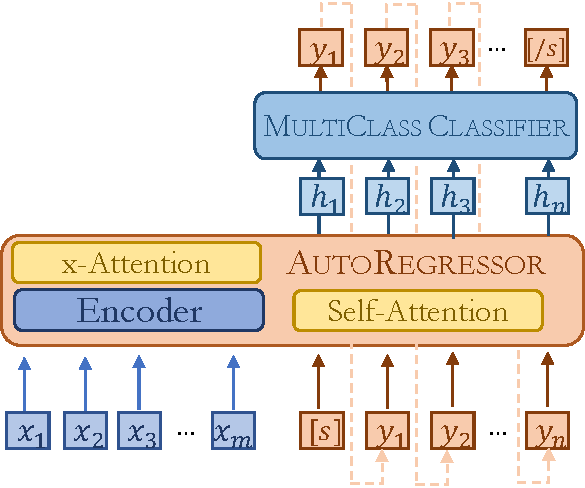
\includegraphics[width=0.65\linewidth]{img/optimvocab/nmt-arch-classifier-new}
    \caption{The NMT model re-envisioned as a token classifier with an autoregressive feature extractor.}
    \label{fig:nmt-architecture}
%% to edit this, go to https://docs.google.com/drawings/d/1Ei9m3WanLJRvoegurFZpiSRQTz7p1Mmde25G0ZwnmAU/edit 
\end{figure}

Autoregressor $R$, \cite{box2015time} being the most complex component of the NMT model, has many implementations based on various neural network architectures: recurrent neural networks (RNN) such as long short-term memory (LSTM) and gated recurrent unit (GRU), convolutional neural networks (CNN), and Transformer. 
At time step $t$, $R$ transforms the input context $y_{<t}, x_{1:m}$ into hidden state vector $h_t = R(y_{<t}, x_{1:m})$.

Classifier $C$ is the same across all architectures.
It maps $h_t$ to a distribution $P(y_j | h_t) \forall y_j \in V_Y$, where $V_Y$ is the vocabulary of $Y$. 
Input to classifiers such as $C$ is generally described as features that are either hand-engineered or automatically extracted.
In our high-level view of NMT architectures, $R$ is a neural network that serves as an automatic feature extractor for $C$.

\subsection{Balanced Classes for Token Classifier}
\label{sec:classifier-balance}

Untreated, class imbalance leads to bias based on class frequencies.
Specifically, classification learning algorithms focus on frequent classes while paying relatively less importance to infrequent classes.
Frequency-based bias leads to poor recall of infrequent classes \cite{Johnson2019SurveyImbalance}. 

When a model is used in a \textit{domain mismatch} scenario, i.e., where test and training set distributions do not match, model performance generally degrades.
It is not surprising that frequency-biased classifiers show particular degradation in domain mismatch scenarios, as  types that were infrequent in the training distribution and were ignored by the learning algorithm may appear with high frequency in the new domain.
\citet{koehn2017sixchallenges} showed empirical evidence of poor generalization of NMT to out-of-domain datasets.

In other classification tasks, where each instance is classified independently, methods such as up-sampling infrequent classes and down-sampling frequent classes are used.
In NMT, since classification is done within the context of sequences, it is possible to accomplish the objective of balancing by altering sequence lengths.
This can be done by choosing the level of subword segmentation \cite{sennrich-etal-2016-bpe}.

\textbf{Quantification of Zipfian Imbalance:}
We use two statistics to quantify the imbalance of a training distribution:

The first statistic relies on a measure of \textbf{Divergence} ($D$) from a balanced (uniform) distribution. 
We use a simplified version of Earth Mover Distance, in which the total cost for moving a probability mass between any two classes  is the sum of the total mass moved.
Since any mass moved \textit{out of} one class is moved \textit{into} another, we divide the total per-class mass moves in half to avoid double counting.  
Therefore, the imbalance measure $D$ on $K$ class distributions where $p_i$ is the observed probability of class $i$ in the training data is computed as:
$$D = \frac{1}{2} \sum_{i=1}^{K}| p_i - \frac{1}{K}|; \quad 0 \le D \le 1 $$

A lower value of $D$ is the desired setting for $C$, since the lower value results from a balanced class distribution. 
When classes are balanced, they have approximately equal frequencies; $C$ is thus less likely to make errors due to class bias.

The second statistic is \textbf{Frequency at 95th\% Class Rank (\textbf{$F_{95\%}$})}, defined as the least frequency in the $95^{th}$ percentile of most frequent classes.
More generally, $F_{\large{P\%}}$ is a simple way of quantifying the minimum number of training examples for at least the $P$th percentile of classes.
The bottom $(1-P)$ percentile of classes are ignored to avoid the noise that is inherent in the real-world natural-language datasets.

A higher value for $F_{95\%}$ is the desired setting for $C$, as a higher value indicates the presence of many training examples per class, and ML methods are known to perform better when there are many examples for each class.  


\subsection{Shorter Sequences for Autoregressor}
\label{sec:ar-short-seq}

Every autoregressive model is an approximation; some may be better than others, but no model is perfect. 
The total error accumulated grows in proportion to the length of the sequence.
These accumulated errors alter the prediction of subsequent tokens in the sequence.
Even though beam search attempts to mitigate this, it does not completely resolve it.  
These challenges with respect to long sentences and beam size are examined by \citet{koehn2017sixchallenges}.


We summarize sequence lengths using \textbf{Mean Sequence Length}, $\mu$, 
computed trivially as the arithmetic mean of the lengths of \textit{target} language sequences after encoding them:
$\mu = \frac{1}{N} \sum_{i=1}^N |y^{(i)}|$
where $y^{(i)}$ is the $i$th sequence in the training corpus of $N$ sequences.
Since shorter sequences have relatively fewer places where an imperfectly approximated autoregressor model can make errors, a smaller $\mu$ is a desired setting for $R$.

%%%%%%%%%%%%%%%%%%%%%%%%%%%%%%%%%%%%%%%%%%%%%%%%%
\subsection{Choosing the Vocabulary Size Systematically}
\label{sec:bpe}

BPE~\cite{sennrich-etal-2016-bpe} is a greedy iterative algorithm often used to segment a vocabulary into useful \textit{subwords}. 
The algorithm starts with characters as its initial vocabulary.
In each iteration, it greedily selects the most frequent type bigram in the training corpus, and replaces the sequence with a newly created compound type.
Once the subword vocabulary is learned, it can be applied to a corpus by greedily segmenting words with the longest available subword type. These operations have an effect on $D$, $F_{95\%}$, and $\mu$.

\textbf{Effect of BPE on $\mu$}:
BPE expands rare words into two or more subwords, lengthening a sequence (and raising $\mu$) relative to simple white-space segmentation.
BPE merges frequent-character sequences into one subword piece, shortening a sequence (and lowering $\mu$) relative to character segmentation.
Hence, the sequence length of BPE segmentation lies in between the sequence lengths obtained by white-space and character-only segmentation methods \cite{morishita-etal-2018-improving}. 

\textbf{Effect of BPE on $F_{95\%}$ and $D$}:
Whether BPE is viewed as a merging of frequent subwords into a relatively less frequent compound, or a splitting of rare words into relatively frequent subwords, BPE alters the class distribution by moving the probability mass of classes.
Hence, by altering the class distribution, BPE also alters both $F_{95\%}$ and $D$. The BPE hyperparameter controls the amount of probability mass moved between subwords and compounds.

Figure~\ref{fig:BPE-imbalance} shows the relation between number of BPE merges (i.e. the BPE hyperparameter), and both $D$ and $\mu$.
When few BPE merge operations are performed, we observe the lowest value of $D$, which is a desired setting for $C$, but at the same point $\mu$ is large and undesired for $R$ (Section~\ref{sec:classifier-nlg}).
When a large number of BPE merges are performed, the effect is reversed, i.e. we observe that $D$ is large and unfavorable to $C$ while $\mu$ is small and favorable to $R$. 
In the following sections we describe our experiments and analysis to locate the optimal number of BPE merges that achieves the right trade-off for both $C$ and $R$. 

 \begin{figure}[ht]
  \centering
    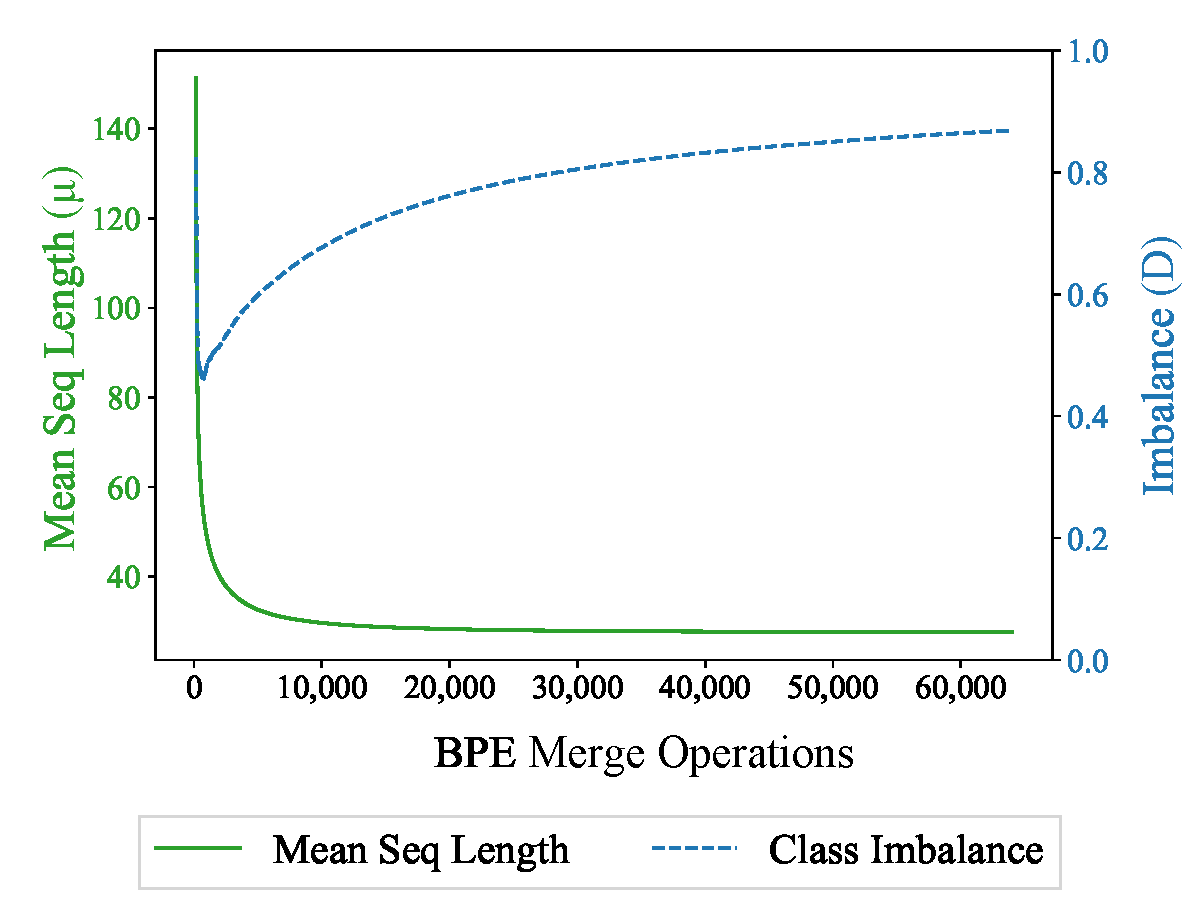
\includegraphics[width=0.7\linewidth]{bpe64k-deen-en.pdf}
    \caption{Effect of BPE merge operations on mean sequence length ($\mu$) and class imbalance ($D$).
    } 
    \label{fig:BPE-imbalance}
\end{figure}


\section{Experimental Setup}
\label{sec:exp-setup}

Our NMT experiments use the base Transformer model \cite{vaswani-2017-attention} on four different target languages at various training data sizes, described in the following subsections. 

\subsection{Datasets}
We use the following four language pairs for our analysis: English$\rightarrow$German, German$\rightarrow$English, English$\rightarrow$Hindi, and English$\rightarrow$Lithuanian. 
To analyze the impact of different training data sizes, we randomly sub-select smaller training corpora for English$\leftrightarrow$German and English$\rightarrow$Hindi language pairs. 
Statistics regarding the corpora used for validation, testing, and training are in Table~\ref{tab:datasets}.
The datasets for English$\leftrightarrow$German, and English$\rightarrow$Lithuanian are retrieved from the News Translation task of WMT2019~\cite{wmt19proceedings}.\footnote{\href{http://www.statmt.org/wmt19/translation-task.html}{http://www.statmt.org/wmt19/translation-task.html}}
For English$\rightarrow$Hindi, we use the IIT Bombay Hindi-English parallel corpus v1.5~\cite{kunchukuttan-etal-2018-iit}.
English, German, and Lithuanian sentences are tokenized using \textsc{SacreMoses}.\footnote{\href{https://github.com/alvations/sacremoses}{https://github.com/alvations/sacremoses}} 
Hindi sentences are tokenized using \textsc{IndicNlpLibrary}.\footnote{\href{https://github.com/anoopkunchukuttan/indic_nlp_library}{https://github.com/anoopkunchukuttan/indic\_nlp\_library}}

The training datasets are trivially cleaned: we exclude sentences with length in excess of five times the length of their parallel counterparts. 
Since the vocabulary is a crucial part of this analysis, we exclude all sentence pairs containing URLs. 

\begin{table*}[ht]
    \centering
    \setlength{\tabcolsep}{3pt}
\begin{tabular}{ l  : l  : r  r  r  : l : l }
  Languages & Training & Sentences & EN Toks & XX Toks & Validation & Test \\ \hline
\multirow{4}{1.5cm}{DE$\rightarrow$EN\\EN$\rightarrow$DE} 
    & \multirow{4}{4cm}{Europarl v10 \\ WMT13CommonCrawl \\ NewsCommentary v14}
         & 30K  &  0.8M & 0.8M & \multirow{4}{*}{ {\small NewsTest18} }
            & \multirow{4}{*}{ \small{NewsTest19}} \\ \cdashline{3-5}
    &    & 0.5M  & 12.9M & 12.2M &  &  \\ \cdashline{3-5}
    &    & 1M    & 25.7M & 24.3M &  &  \\ \cdashline{3-5} 
    &    & 4.5M  & 116M & 109.8M &  &  \\ \hdashline

\multirow{2}{*}{EN$\rightarrow$HI } 
     & \multirow{2}{*}{ IITB Training } 
         & 0.5M & 8M & 8.6M  & \multirow{2}{*}{ \small{IITB Dev} } 
     & \multirow{2}{*}{ \small{IITB Test} }  \\\cdashline{3-5} 
     &   & 1.3M & 21M & 22.5M   &   &  \\ \hdashline 
EN$\rightarrow$LT & Europarl v10 & 0.6M & 17M & 13.4M  & \small{NewsDev19} & \small{NewsTest19} \\
\end{tabular} 
    \caption{Training, validation, and testing datsets, along with sentence and token counts in training sets. We generally refer to dataset's sentences as size in this chapter.}
    \label{tab:datasets}
\end{table*}

\subsection{Hyperparameters}
Our model is a 6 layer Transformer encoder-decoder that has 8 attention heads, 512 hidden vector units, and a feed forward intermediate size of 2048, with GELU activation. 
We use label smoothing at 0.1, and a dropout rate of 0.1.
We use the Adam optimizer \cite{kingma2015adam} with a controlled learning rate that warms up for 16K steps followed by the decay rate recommended for training Transformer models~\cite{popel2018tfm-train-tips}. 
To improve performance at different data sizes, we set the mini-batch size to 6K tokens for the 30K-sentence datasets, 12K tokens for 0.5M-sentence datasets, and 24K for the remaining larger datasets~\cite{popel2018tfm-train-tips}. 
All models are trained until no improvement in validation loss is observed, with patience of 10 validations, each done at 1,000 update steps apart. 
Our model is implemented using PyTorch and run on NVIDIA P100 and V100 GPUs.
To reduce padding tokens per batch, mini-batches are made of sentences having similar lengths \cite{vaswani-2017-attention}.
We trim longer sequences to a maximum of 512 tokens after BPE.
To decode, we average the last 10 checkpoints, and use a beam size of 4 with length penalty of 0.6, similar to \citet{vaswani-2017-attention}.

Since the vocabulary size hyperparameter is the focus of this analysis, we use a range of vocabulary sizes that include character vocabulary and BPE operations that yield vocabulary sizes between 500 and 64K types.
A common practice, as seen in \citet{vaswani-2017-attention}'s setup, is to jointly learn BPE for both source and target languages, which facilitates three-way weight sharing between the encoder's input, the decoder's input, and the output (i.e., classifier's class) embeddings \cite{press-wolf-2017-embeddings}.
However, to facilitate fine-grained analysis of vocabulary sizes and their effect on class imbalance, our models separately learn source and target vocabularies; weight sharing between the encoder's and decoder's embeddings is thus not possible.
For the target language, however, we share weights between the decoder's input and the classifier's class embeddings.

\section{Results and Analysis}
\label{sec:nmt_analysis}

\begin{figure}[h!t]
\centering
\begin{subfigure}{\linewidth}
    \centering
    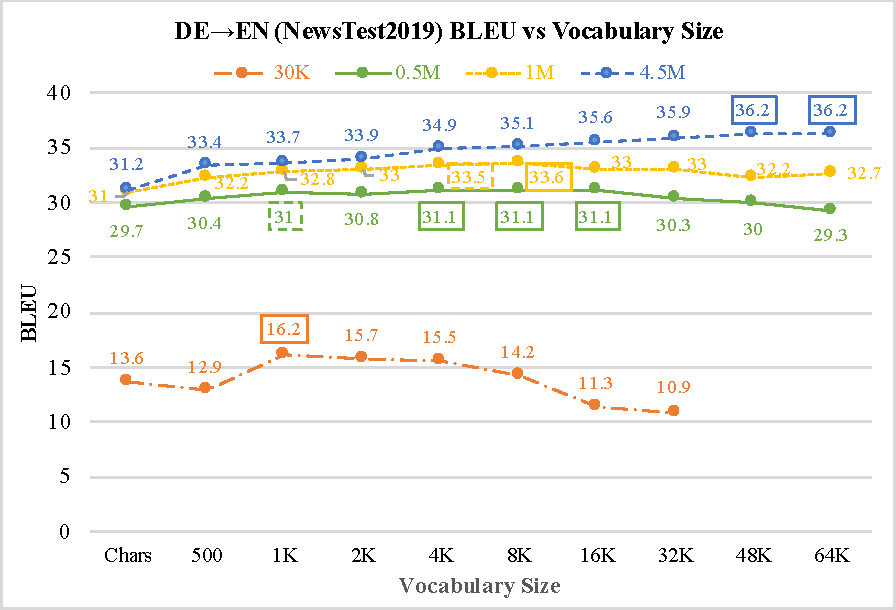
\includegraphics[width=0.7\linewidth]{bleu-deen.pdf}
    \caption{DE$\rightarrow$EN BLEU on NewsTest2019}
    \label{fig:bleu-deen}
\end{subfigure}

\vspace{5mm}

\begin{subfigure}{\linewidth}
    \centering
    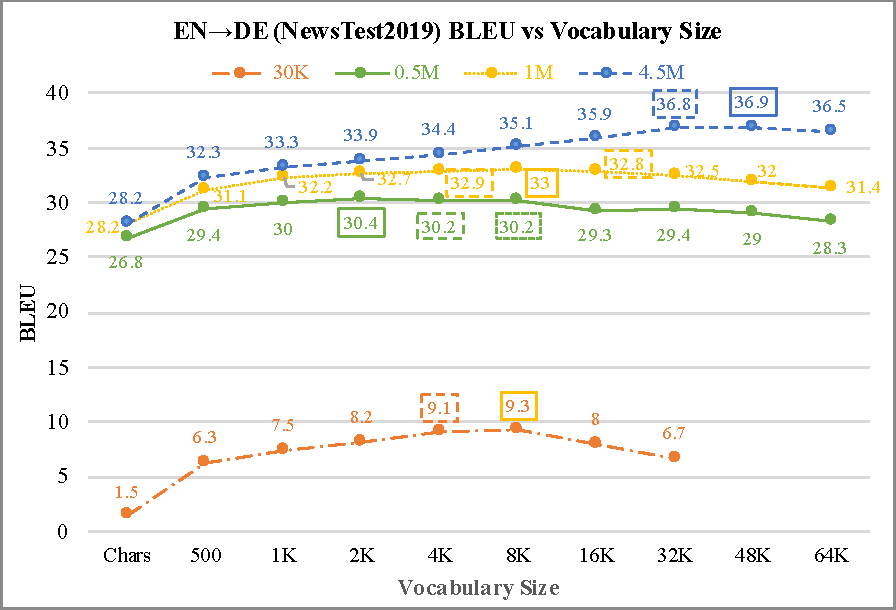
\includegraphics[width=0.7\linewidth]{bleu-ende.pdf}
    \caption{EN$\rightarrow$DE BLEU on NewsTest2019}
    \label{fig:bleu-ende}
\end{subfigure}
\caption{EN$\leftrightarrow$DE NewsTest2019 BLEU as a function of vocabulary size at various training set sizes. 
Only the large dataset with 4.5M sentences has its best performance at a large vocabulary; all others peak at an 8K or smaller vocabulary size.}
\label{fig:bleu-ende-deen}
\end{figure}

\begin{figure}[ht]
    \centering    
    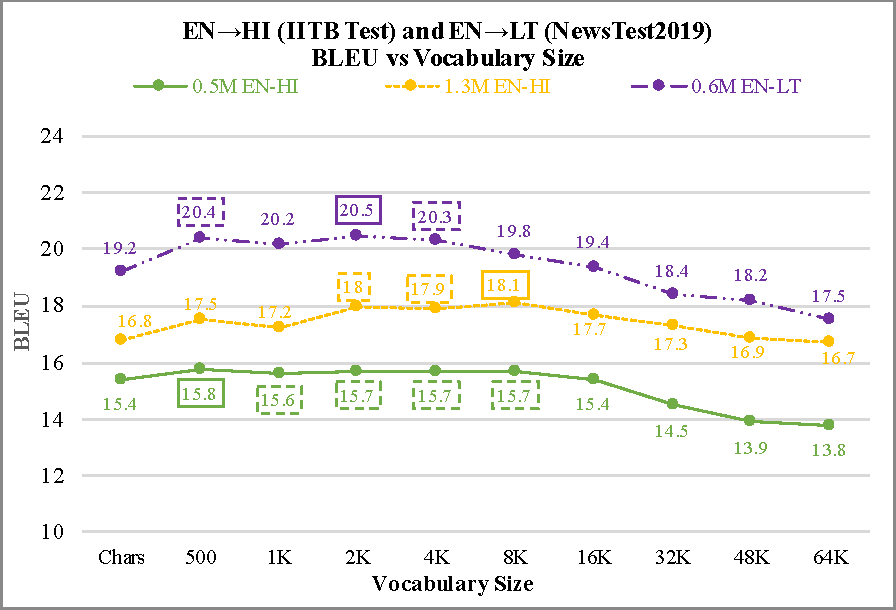
\includegraphics[width=0.7\linewidth]{bleu-enhi-enlt.pdf}
    \caption{BLEU on EN$\rightarrow$HI IITB Test and EN$\rightarrow$LT NewsTest2019 as a function of vocabulary size.
    These language pairs observed the best BLEU scores in the range of 500 to 8K vocabulary size.}
    \label{fig:bleu-enhilt}
\end{figure}

BLEU scores for DE$\rightarrow$EN and EN$\rightarrow$DE experiments are reported in Figures~\ref{fig:bleu-deen} and \ref{fig:bleu-ende} respectively.
Results from EN$\rightarrow$HI, and EN$\rightarrow$LT are combined in Figure~\ref{fig:bleu-enhilt}.
All the reported BLEU scores are obtained using \textsc{SacreBleu} \cite{post-2018-sacrebleu}.\footnote{\texttt{BLEU+case.mixed+numrefs.1+smooth.exp+tok.13a+version.1.4.6}}

We make the following observations: smaller vocabulary such as characters have not produced the best BLEU for any of our language pairs or dataset sizes. 
A vocabulary of 32K or larger is unlikely to produce optimal results unless the data set is large e.g. the 4.5M DE$\leftrightarrow$EN sets.
The BLEU curves as a function of vocabulary sizes have a shape resembling a hill. 
The position of the peak of the hill seems to shift towards a larger vocabulary when the datasets are large. 
However, there is a lot of variance in the position of the peak: one extreme is at 500 types on 0.5M EN$\rightarrow$HI, and the other extreme is at 64K types in 4.5M DE$\rightarrow$EN. 
    
Although Figures~\ref{fig:bleu-ende-deen} and \ref{fig:bleu-enhilt} indicate \textit{where} the optimal vocabulary size is for these chosen language pairs and datasets, the question of \textit{why} the peak is where it is remains unanswered.
We visualize $\mu$, $D$, and $F_{95\%}$ in Figures \ref{fig:mu-d-freq-bleu} and \ref{fig:mu-d-freq-bleu-continued} to answer that question, and report these observations:
\begin{enumerate}
    \itemsep0em 
    \item Small vocabularies have a relatively larger $F_{95\%}$ (favorable to classifier), yet they are suboptimal. We reason that this is due to the presence of a larger $\mu$, which is unfavorable to the autoregressor.
    \item Larger vocabularies such as 32K and beyond have a smaller $\mu$, which favors the autoregressor, yet rarely achieves the best BLEU.
    We reason this is due to the presence of a lower $F_{95\%}$ and a higher $D$ being unfavorable to the classifier.
    Since the larger datasets have many training examples for each class, as indicated by a generally larger $F_{95\%}$, we conclude that bigger vocabularies tend to yield optimal results compared to smaller datasets in the same language.
    
    \item On small (30K) to medium (1.3M) data sizes, the vocabulary size of 8K seems to find a good trade-off between $\mu$ and $D$, as well as between $\mu$ and $F_{95\%}$.
\end{enumerate}

 There is a \textit{simple heuristic} to locate the peak: the near-optimal vocabulary size is where sentence length $\mu$ is small, while $F_{95\%}$ is approximately $100$ or higher.
 
 
 \begin{figure}[h!t]
    \centering
    \begin{subfigure}{0.8\textwidth}
    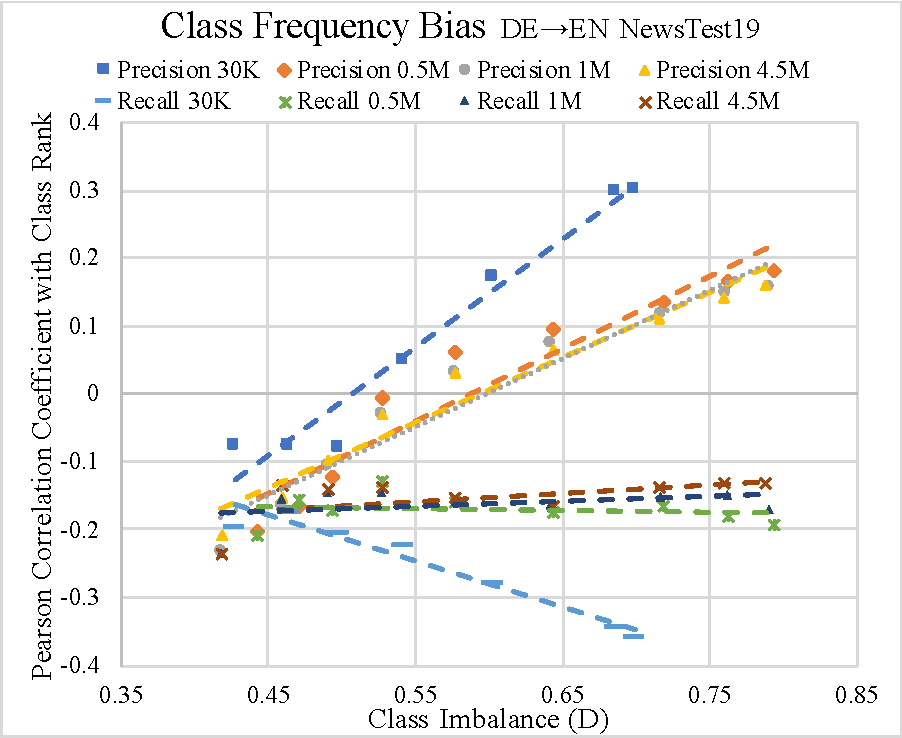
\includegraphics[width=\linewidth]{corr-deen-test.pdf}
    \end{subfigure}
    
    \vspace{5mm}

    \begin{subfigure}{0.8\textwidth}
    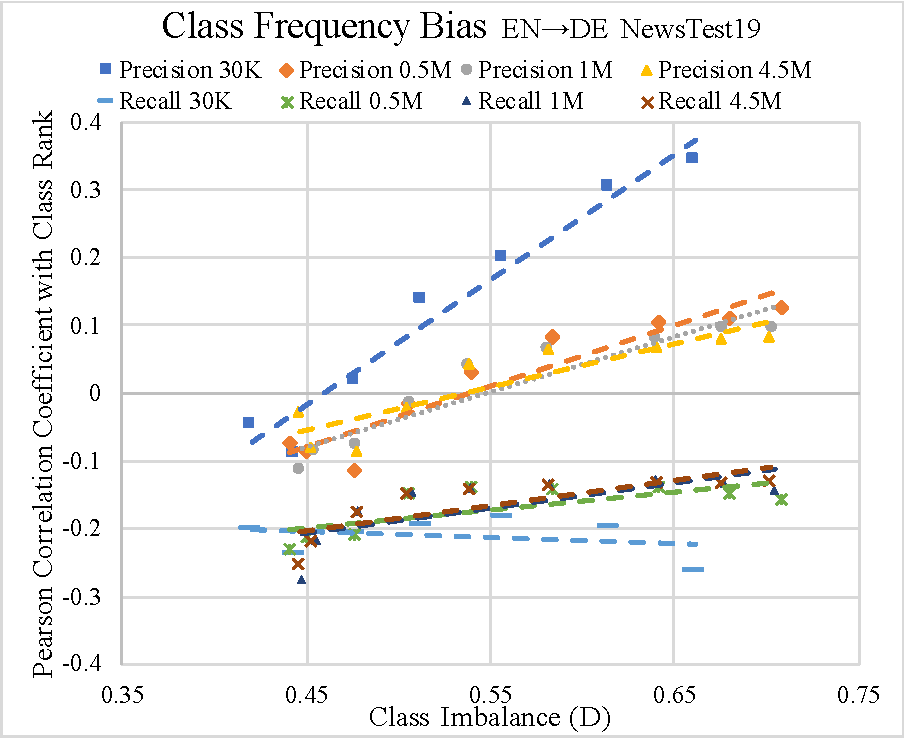
\includegraphics[width=\linewidth]{corr-ende-test.pdf}
    \end{subfigure}
    
    \caption{Correlation analysis on DE$\rightarrow$EN and EN$\rightarrow$DE shows that NMT models suffer from frequency based class bias, indicated by non-zero correlation of both precision and recall with class rank. Reduction in class imbalance (D), as shown by the horizontal axis, generally reduces the bias as indicated by the reduction in magnitude of correlation.}
         \label{fig:corr-deen-test}
\end{figure}
 
 

\begin{figure}[h!t]
\centering
\begin{subfigure}{\textwidth}
  \centering
  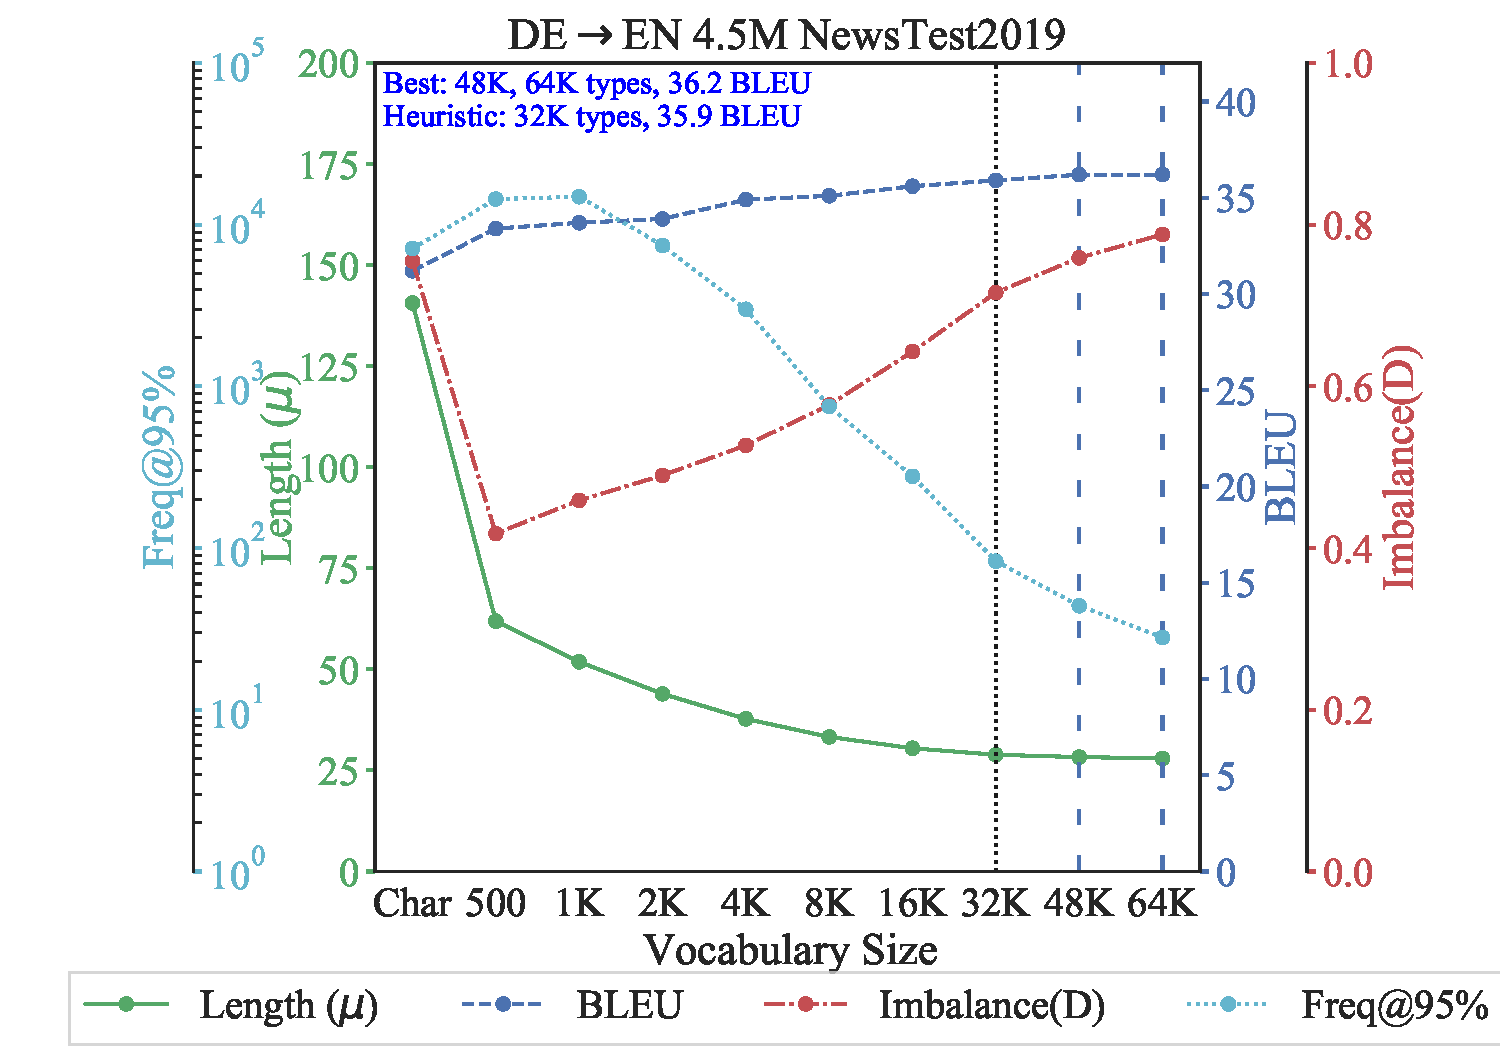
\includegraphics[width=0.7\linewidth,trim={1.4cm 0 0.2cm 16.45cm},clip]{4axv-test-deen-4.5m.pdf}
\end{subfigure}

\vspace{1mm}

\begin{subfigure}{.44\textwidth}
  \centering
  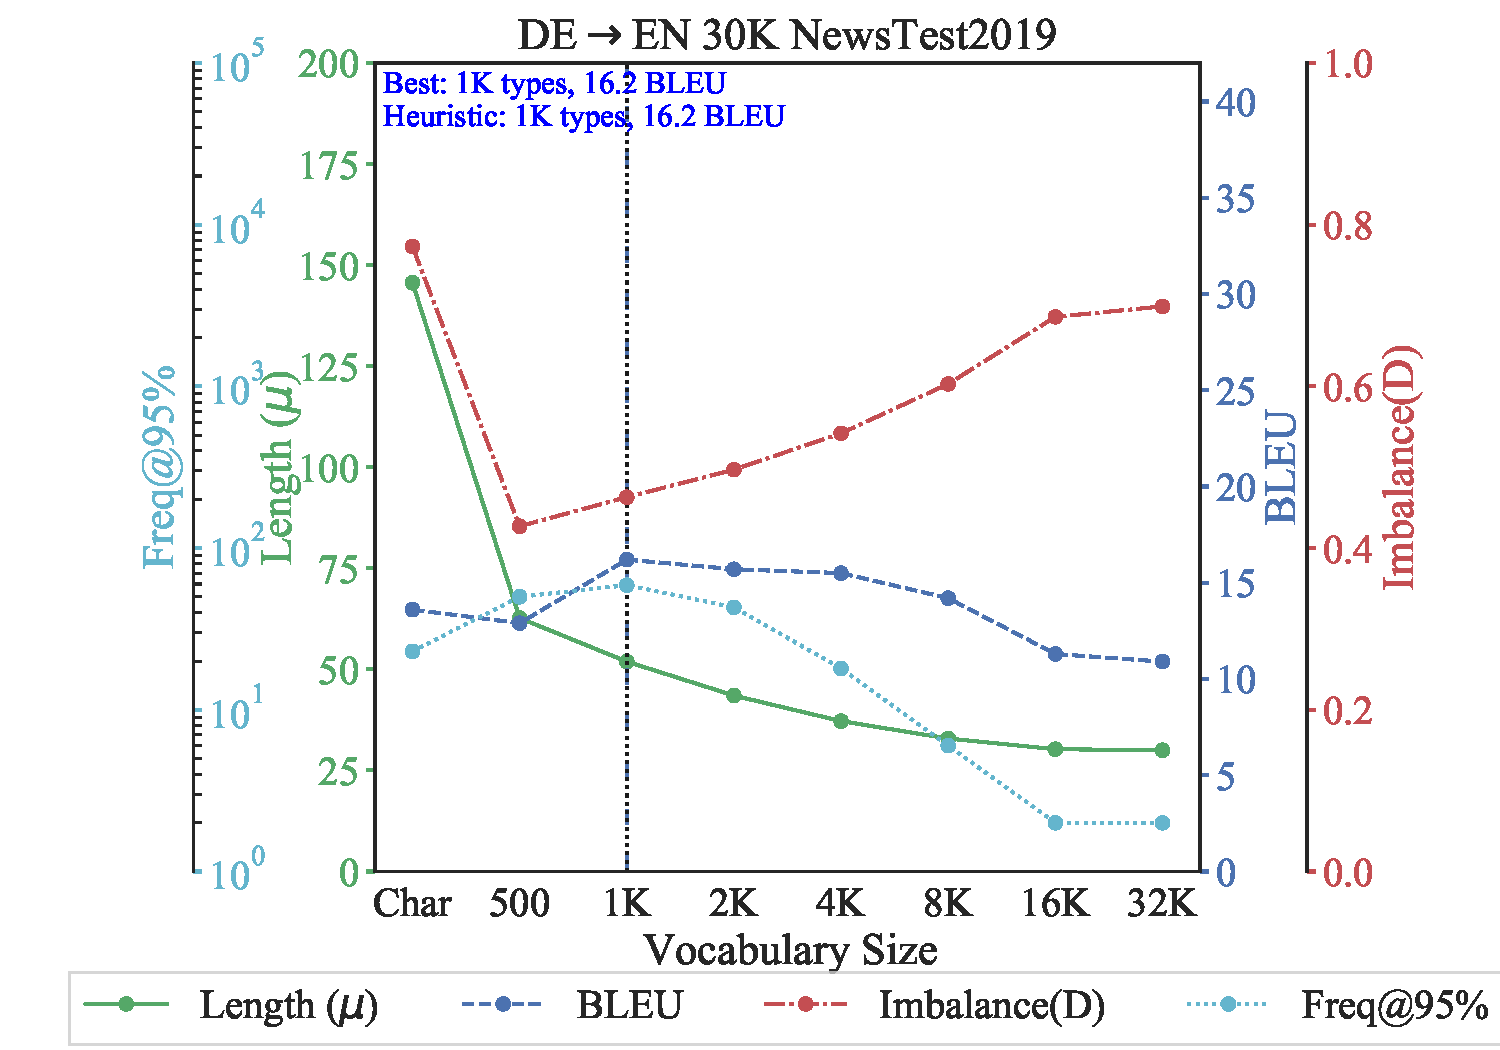
\includegraphics[width=0.99\linewidth,trim={2.4cm 1.32cm 4.1cm 0},clip]{4axv-test-deen-30k.pdf}
  %\caption{1a}
  %\label{fig:sfig1}
\end{subfigure}
\begin{subfigure}{.44\textwidth}
  \centering
  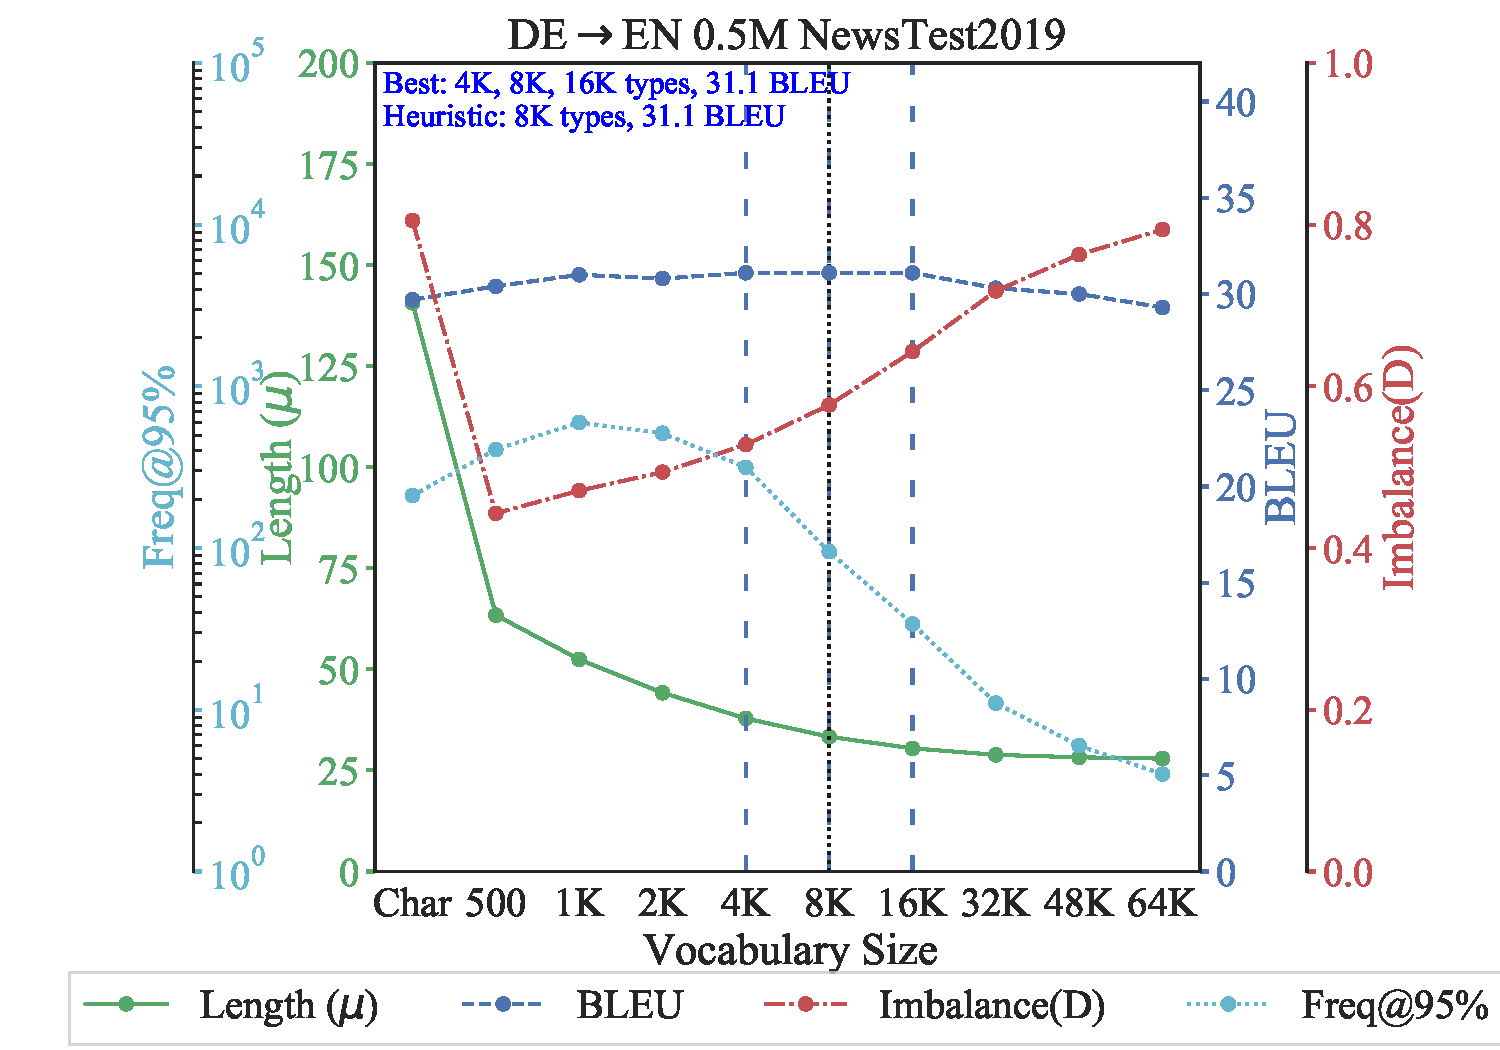
\includegraphics[width=0.99\linewidth,trim={5.1cm 1.32cm 1.4cm 0},clip]{4axv-test-deen-0.5m.pdf}
  %\caption{1c}
  %\label{fig:sfig2}
\end{subfigure}


\begin{subfigure}{.44\textwidth}
  \centering
  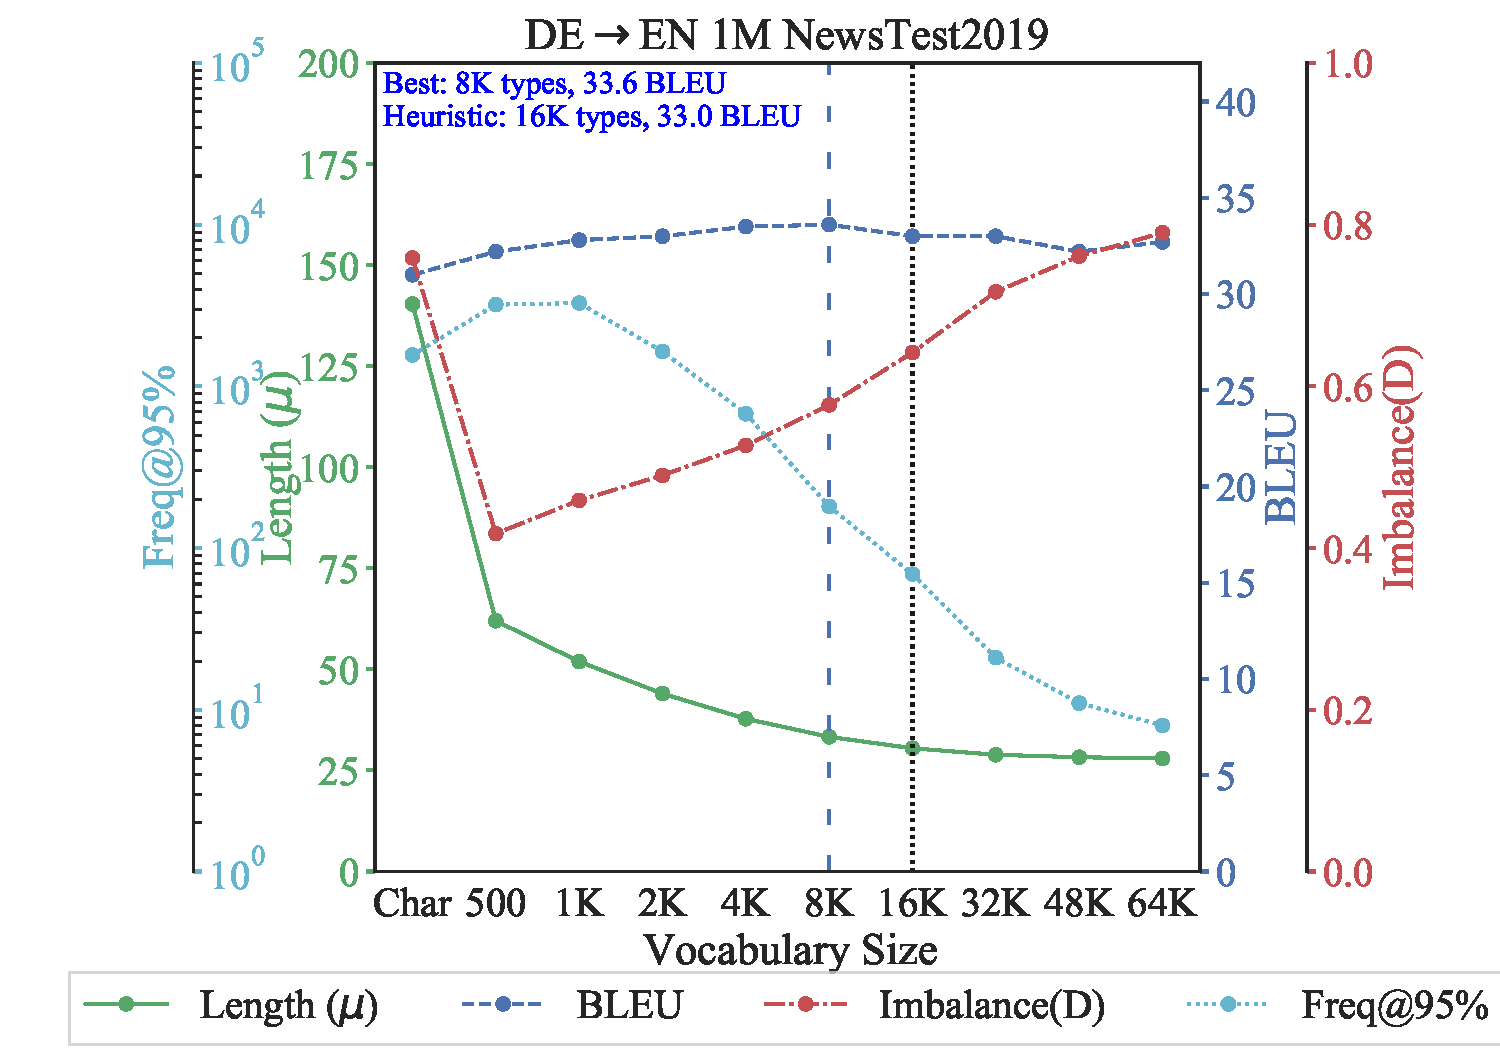
\includegraphics[width=0.99\linewidth,trim={2.4cm 1.32cm 4.1cm 0},clip]{4axv-test-deen-1m.pdf}
  %\caption{1c}
  %\label{fig:sfig2}
\end{subfigure}
\begin{subfigure}{.44\textwidth}
  \centering
  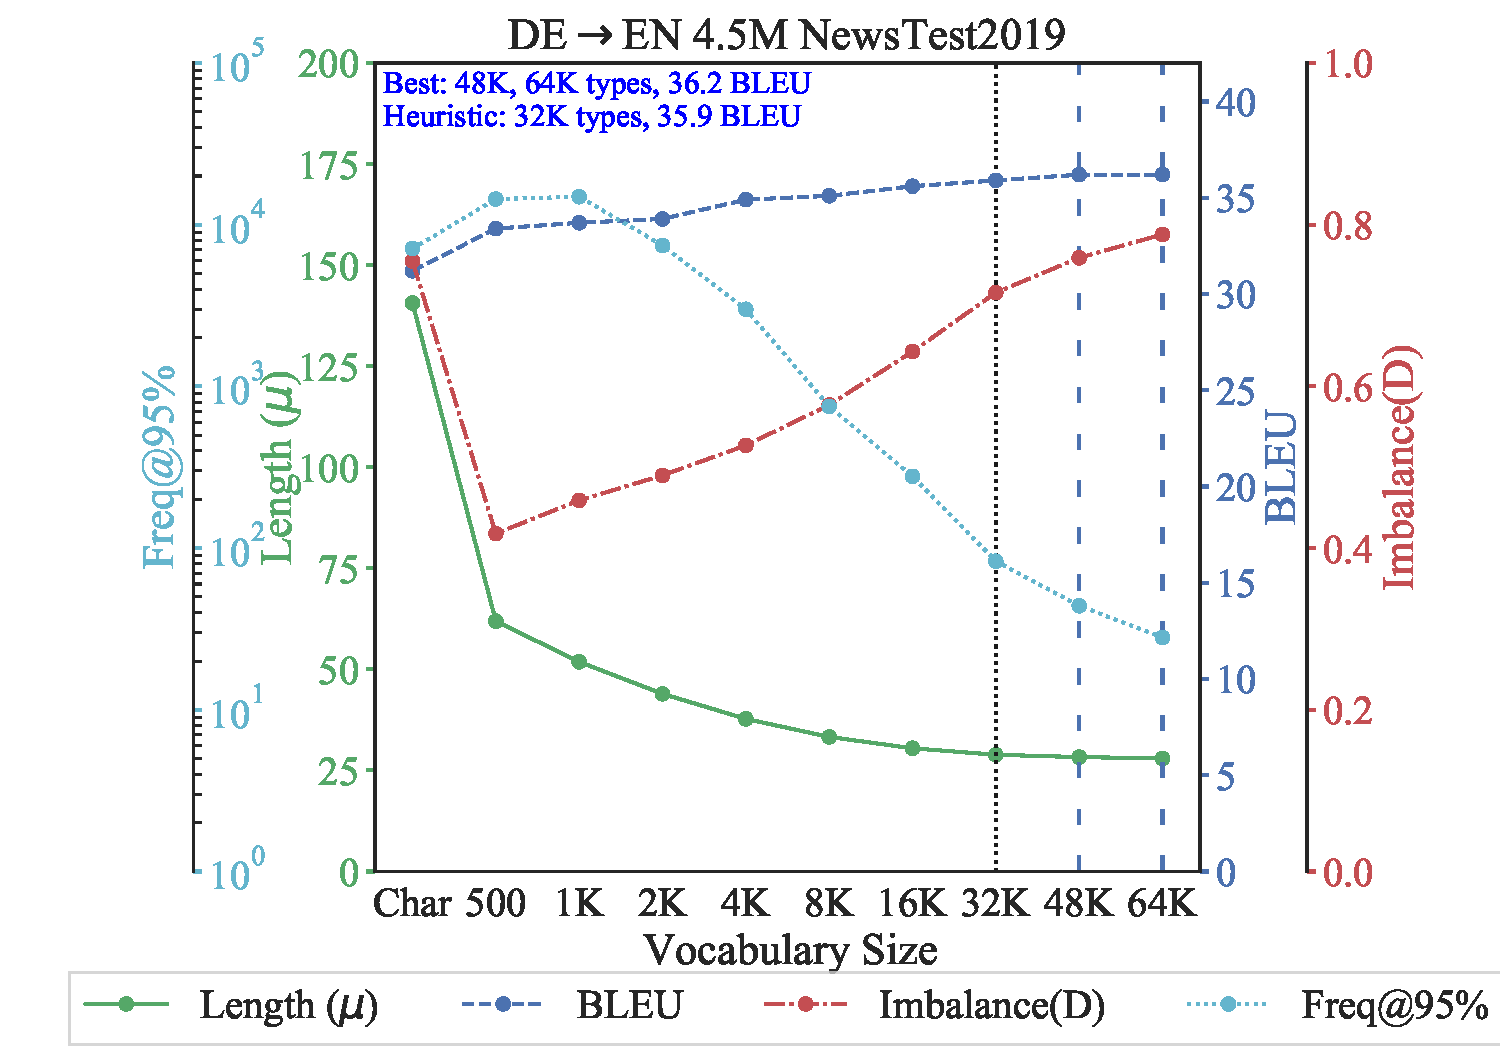
\includegraphics[width=0.99\linewidth,trim={5.1cm 1.32cm 1.4cm 0},clip]{4axv-test-deen-4.5m.pdf}
  %\caption{1c}
  %\label{fig:sfig2}
\end{subfigure}

\begin{subfigure}{.44\textwidth}
  \centering
  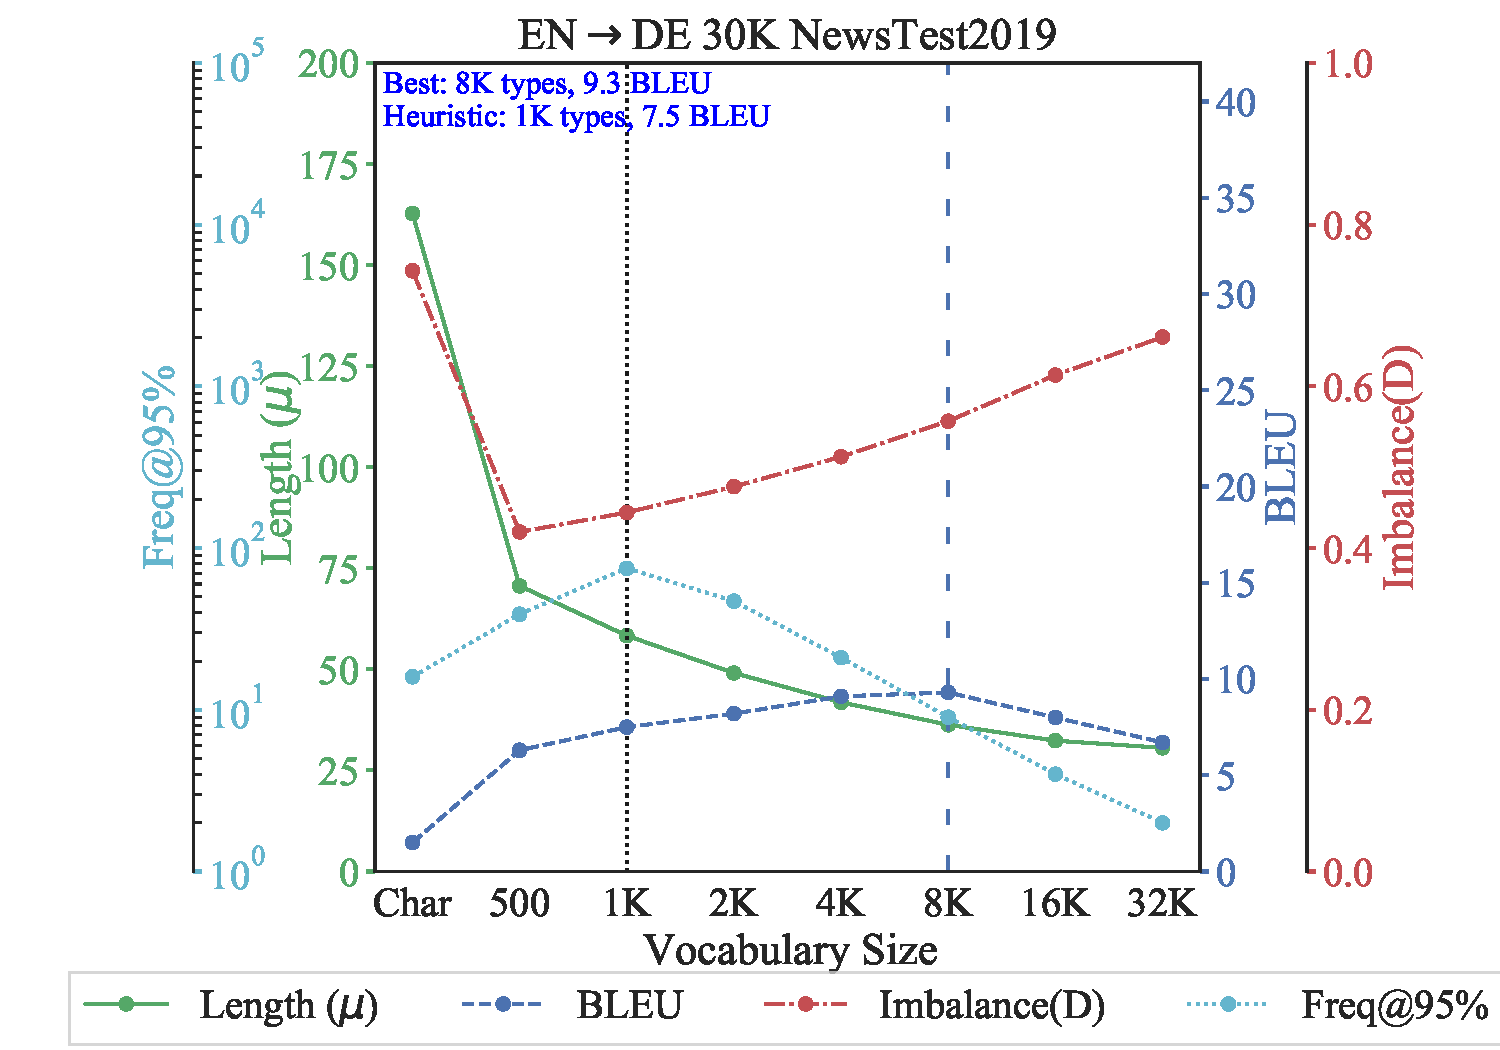
\includegraphics[width=0.99\linewidth,trim={2.4cm 1.32cm 4.1cm 0},clip]{4axv-test-ende-30k.pdf}
 % \caption{1a}
  %\label{fig:sfig1}
\end{subfigure}
\begin{subfigure}{.44\textwidth}
  \centering
  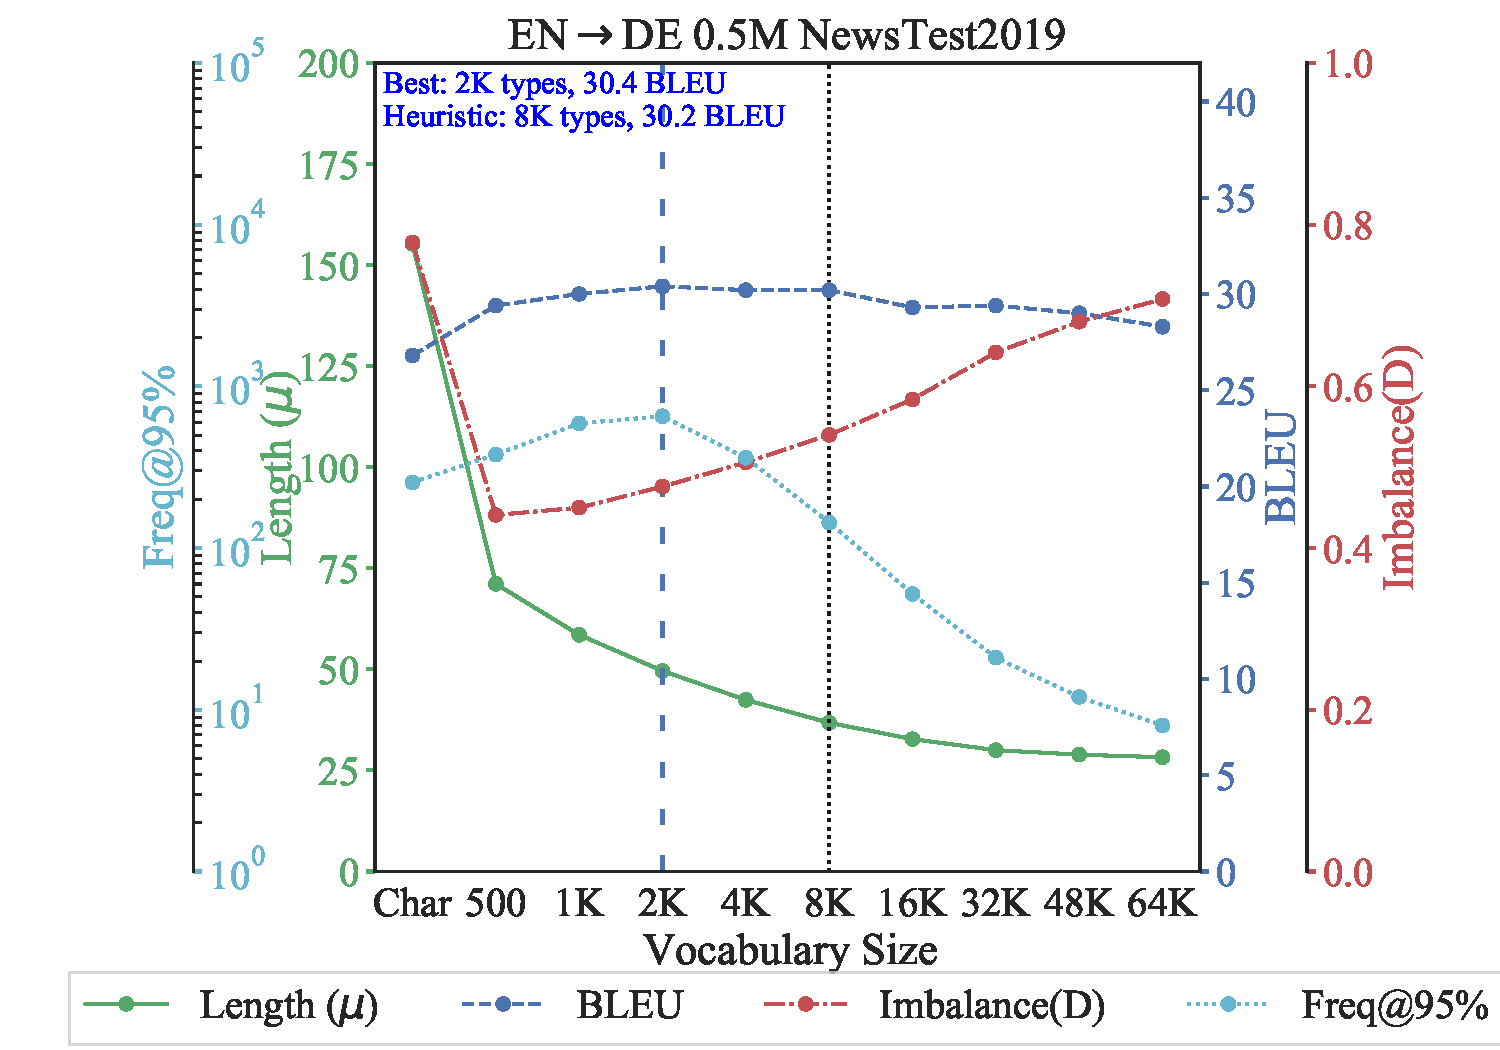
\includegraphics[width=0.99\linewidth,trim={5.1cm 1.32cm 1.4cm 0},clip]{4axv-test-ende-0.5m.pdf}
  %\caption{1c}
  %\label{fig:sfig2}
\end{subfigure}

\caption[Visualization of sequence length, class imbalance, frequency of $95^{th}$ percentile class, and test set BLEU.]{Visualization of sequence length ($\mu$) (lower is better), class imbalance (D) (lower is better), frequency of $95^{th}$ percentile class ($F_{95\%}$) (higher is better; plotted in logarithmic scale), and test set BLEU (higher is better) on all language pairs and training data sizes.
%DE$\leftrightarrow$EN of 1M resembles resembles DE$\leftrightarrow$EN of 0.5M and is provided in Appendix~\ref{sec:appendix} along with visualizations on validation sets.
The vocabulary sizes that achieved highest BLEU are indicated with dashed vertical lines, and the vocabulary our heuristic selects is indicated by dotted vertical lines.}
\label{fig:mu-d-freq-bleu}
\end{figure}

\begin{figure}[h!t]
\ContinuedFloat
\centering

\begin{subfigure}{\textwidth}
  \centering
  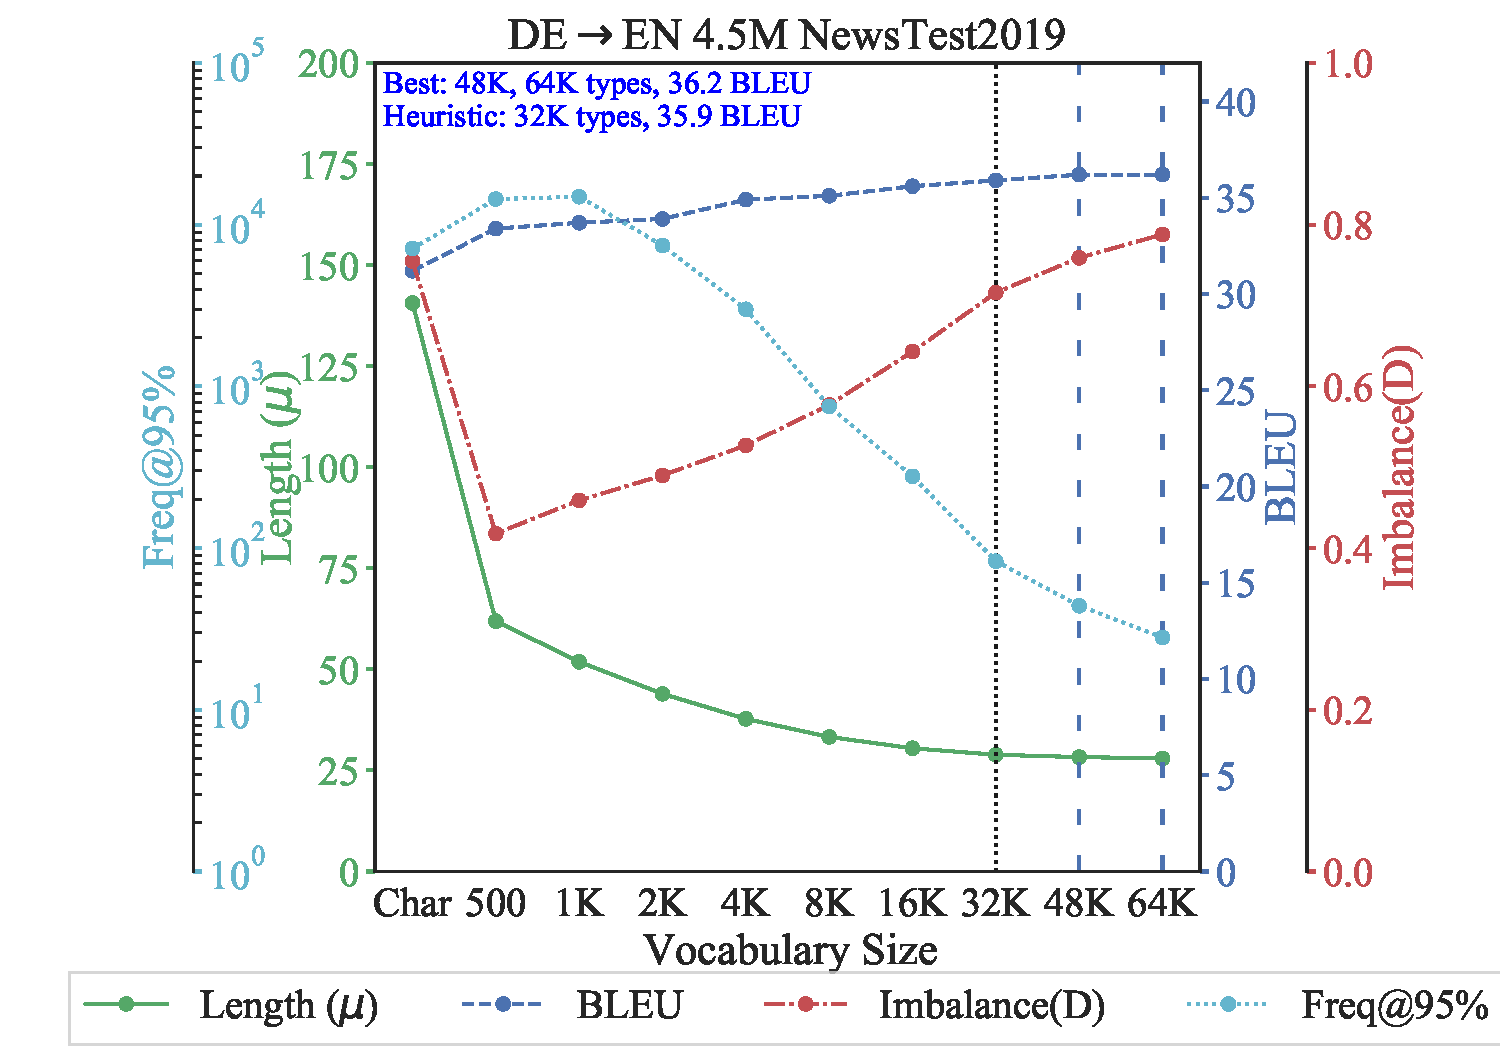
\includegraphics[width=0.7\linewidth,trim={1.4cm 0 0.2cm 16.45cm},clip]{4axv-test-deen-4.5m.pdf}
\end{subfigure}

\vspace{2mm}

\begin{subfigure}{.45\textwidth}
  \centering
  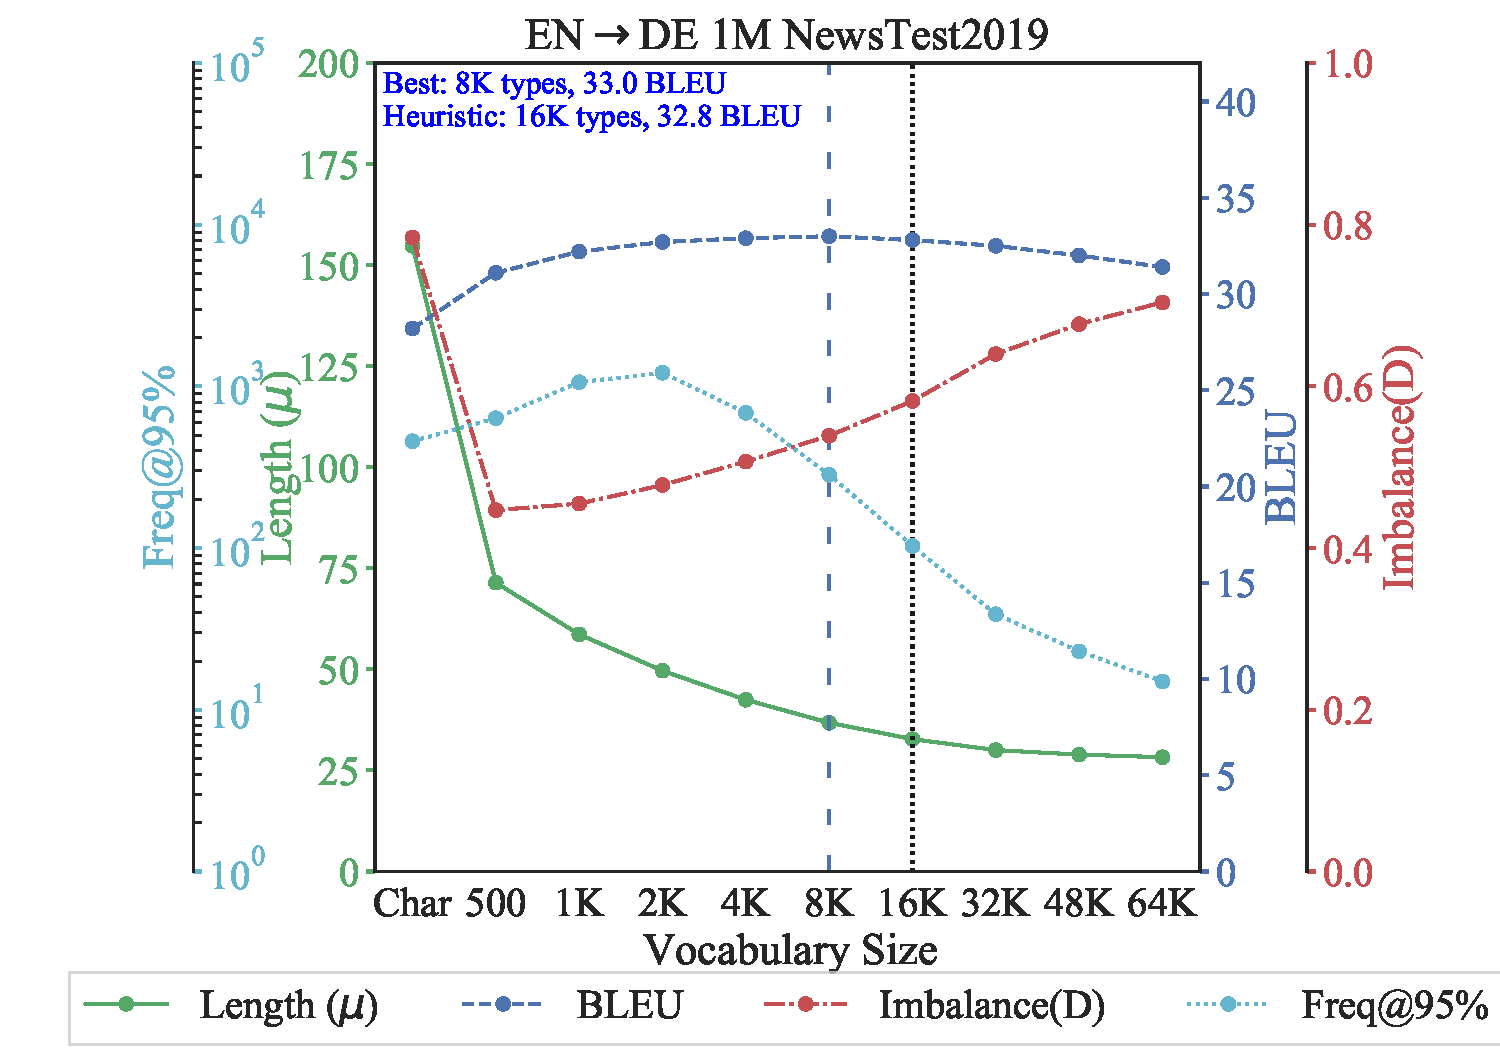
\includegraphics[width=0.99\linewidth,trim={2.4cm 1.32cm 4.1cm 0},clip]{4axv-test-ende-1m.pdf}
 % \caption{1c}
  %\label{fig:sfig2}
\end{subfigure}
\begin{subfigure}{.45\textwidth}
  \centering
  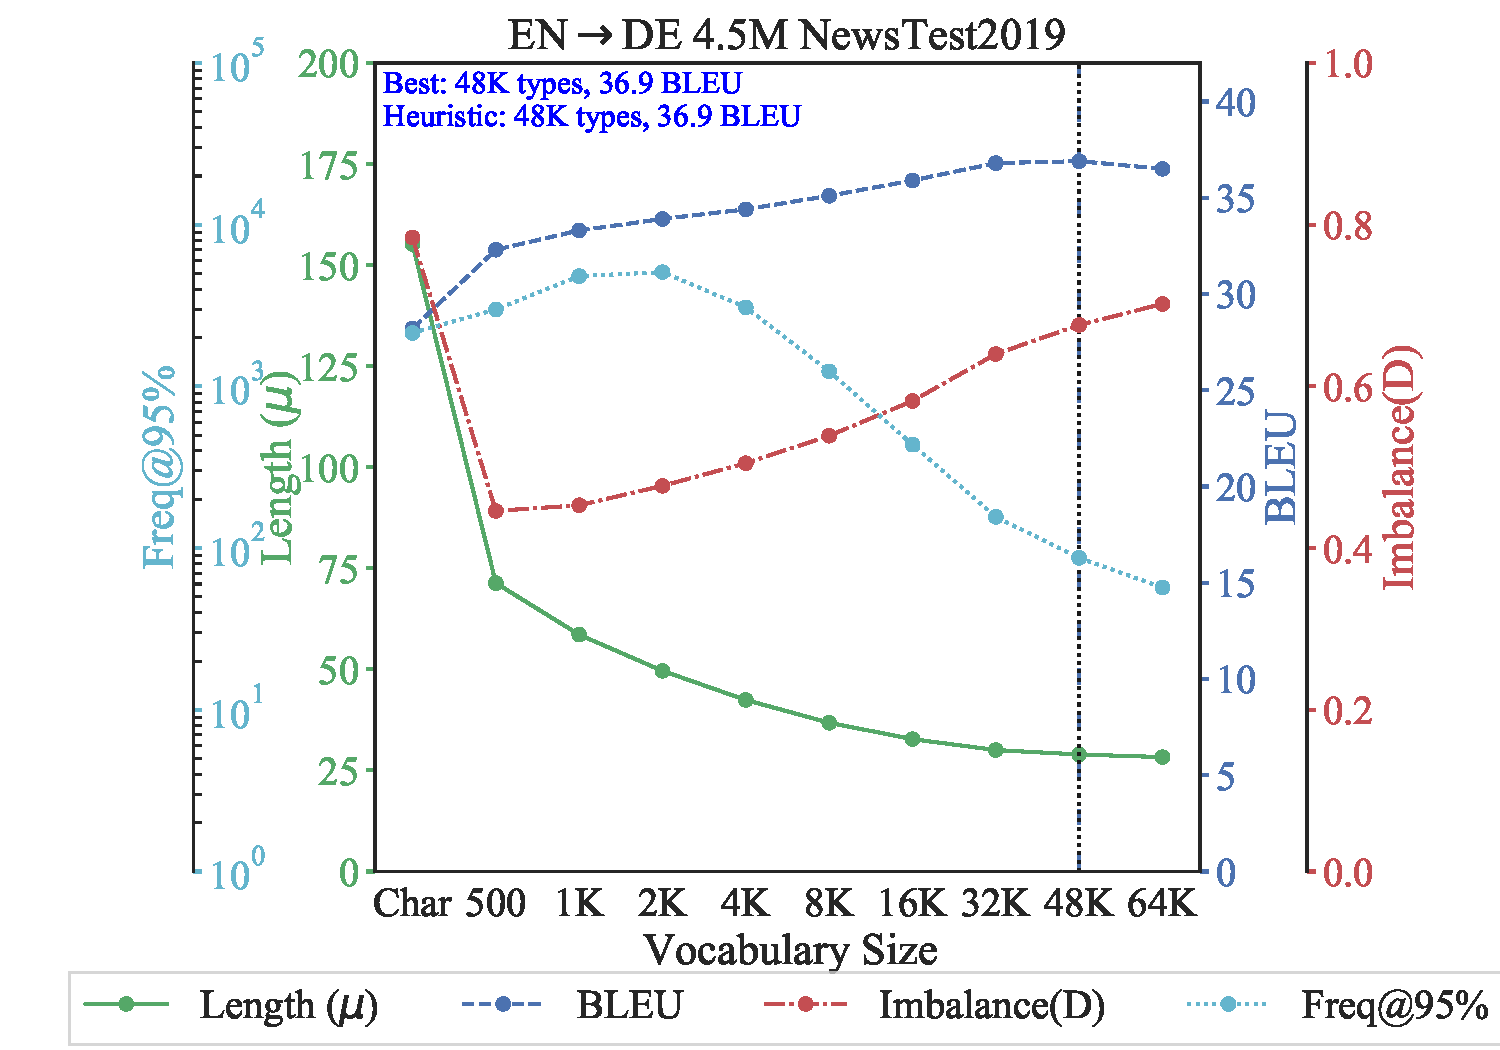
\includegraphics[width=0.99\linewidth,trim={5.1cm 1.32cm 1.4cm 0},clip]{4axv-test-ende-4.5m.pdf}
 % \caption{1c}
  %\label{fig:sfig2}
\end{subfigure}


\begin{subfigure}{.45\textwidth}
  \centering
  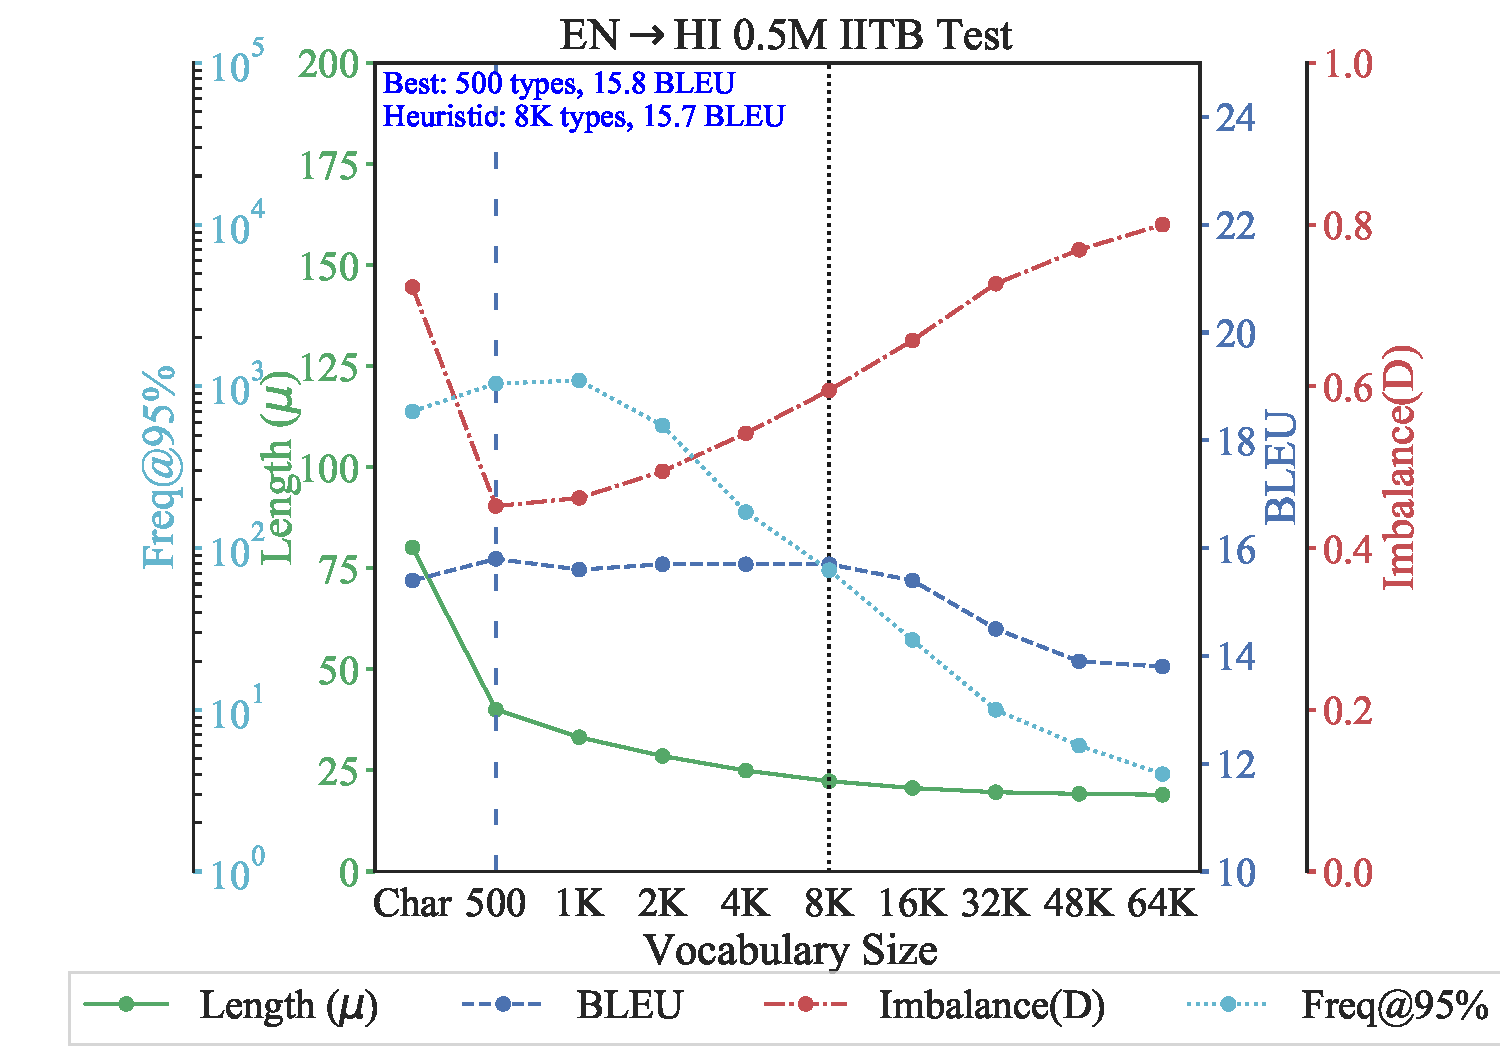
\includegraphics[width=0.99\linewidth,trim={2.4cm 1.32cm 4.1cm 0},clip]{4axv-test-enhi-0.5m.pdf}
 % \caption{1a}
  %\label{fig:sfig1}
\end{subfigure}
\begin{subfigure}{.45\textwidth}
  \centering
  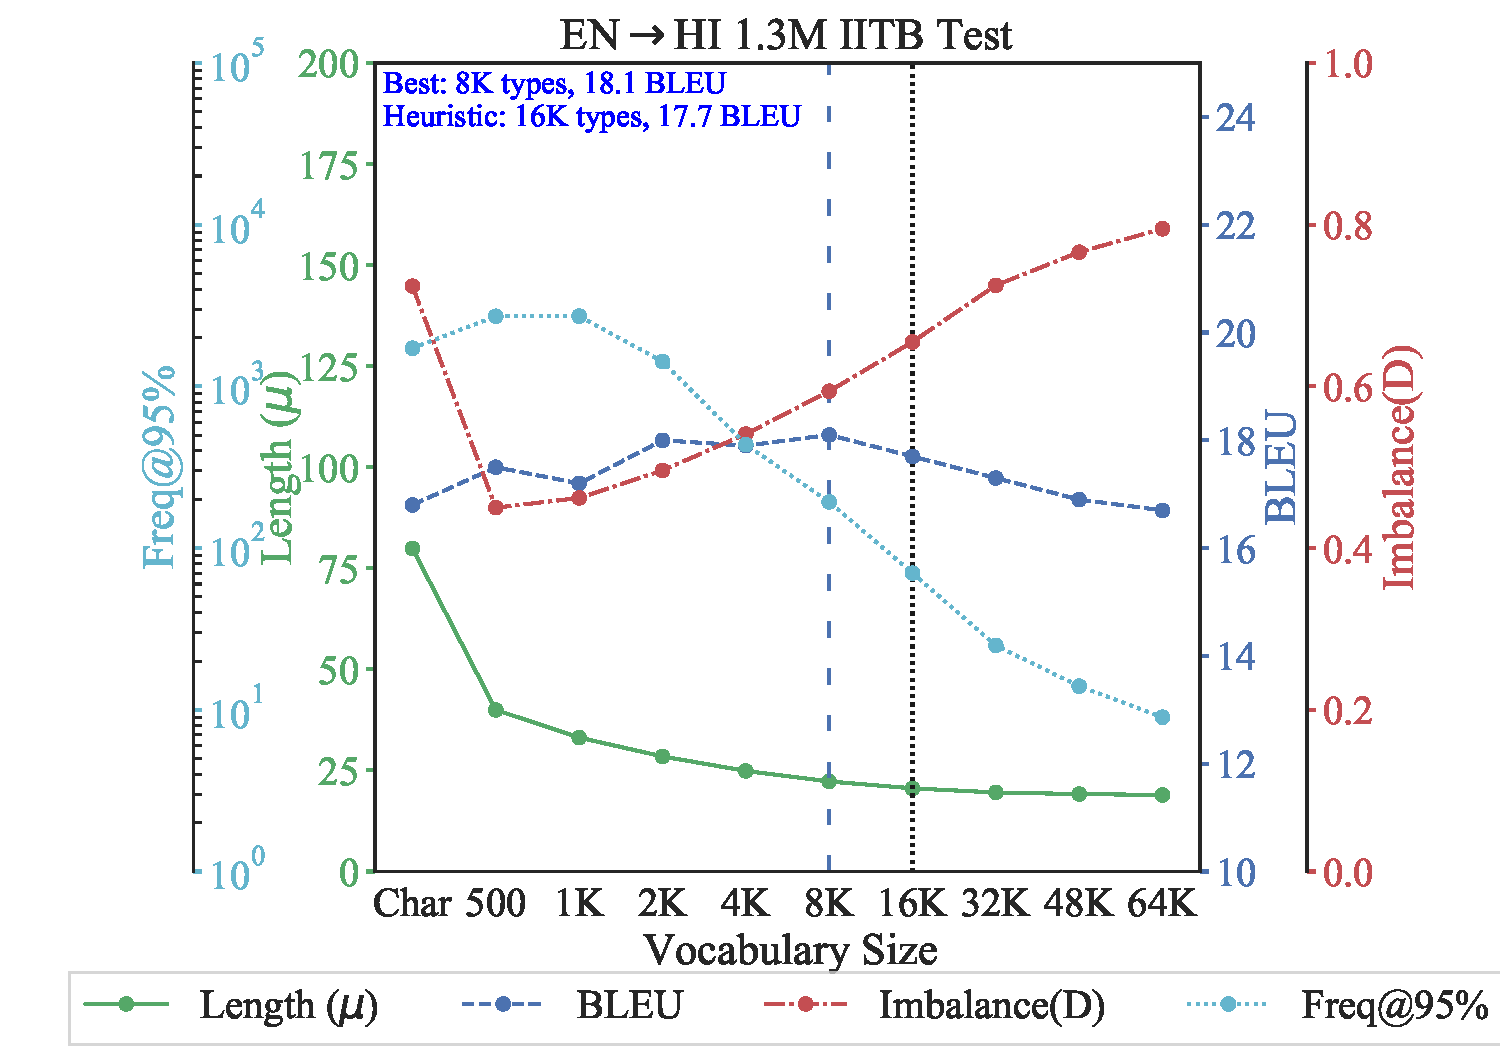
\includegraphics[width=0.99\linewidth,trim={5.1cm 1.32cm 1.4cm 0},clip]{4axv-test-enhi-1.3m.pdf}
  %\caption{1c}
  %\label{fig:sfig2}
\end{subfigure}

\begin{subfigure}{.54\textwidth}
  \centering
  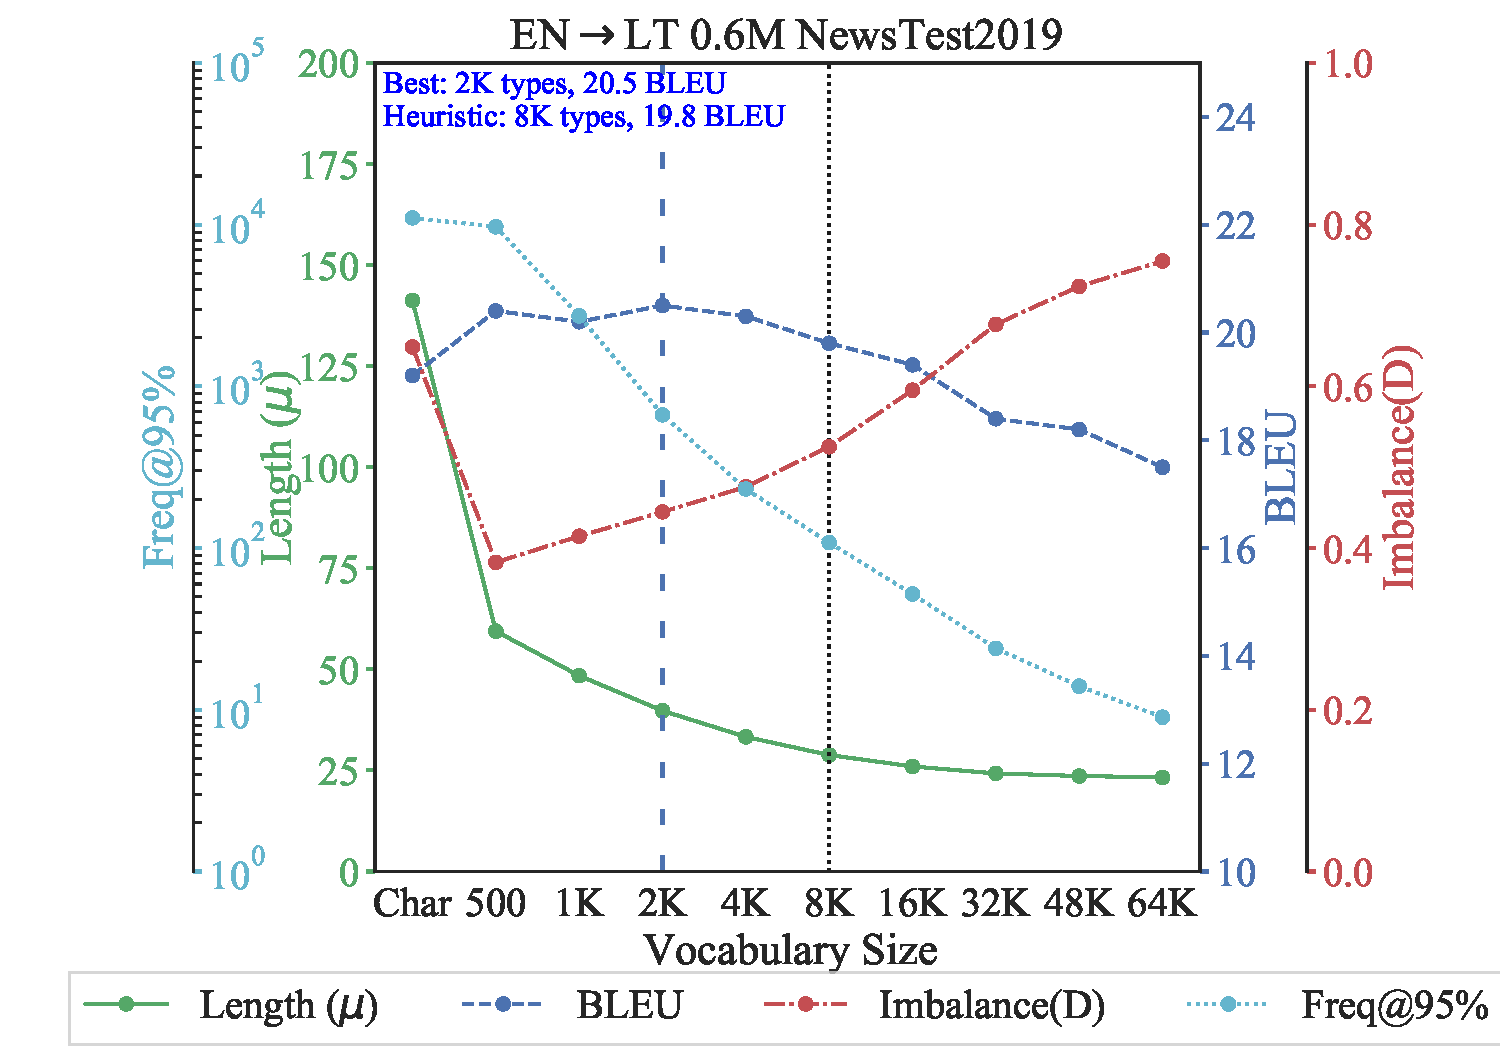
\includegraphics[width=0.99\linewidth,trim={2.4cm 1.32cm 1.4cm 0},clip]{4axv-test-enlt-0.6m.pdf}
  %\caption{1c}
  %\label{fig:sfig2}
\end{subfigure}

\caption{Continuation of Figure~\ref{fig:mu-d-freq-bleu} (see previous page for caption)}
\label{fig:mu-d-freq-bleu-continued}
\end{figure}

BLEU scores are often lower at larger vocabulary sizes---where $\mu$ is (favorably) low but $D$ is (unfavorably) high (Figure~\ref{fig:mu-d-freq-bleu}). This calls for a further investigation that is discussed in the following section.

\section{Measuring Classifier Bias Due to Imbalance}
\label{sec:class-bias}

In a typical classification setting with imbalanced classes, the classifier learns an undesired bias based on frequencies. 

A balanced class distribution debiases in this regard, leading to improvement in the precision of frequent classes as well as recall of infrequent classes.
However, BLEU focuses only on the \textit{precision} of classes; except for adding a global brevity penalty, it is ignorant of the poor recall of infrequent classes. 

Therefore, the BLEU scores shown in Figures~\ref{fig:bleu-deen}, \ref{fig:bleu-ende} and \ref{fig:bleu-enhilt} capture only a part of the improvements and biases. 
In this section, we perform a detailed analysis of the impact of class balancing by considering both precision \textit{and} recall of classes. 

We accomplish this in two stages:
First, we define a method to measure the bias of the model for classes based on their frequencies.
Second, we track the bias in relation to vocabulary size and class imbalance, and report DE$\rightarrow$EN, as it has many data points.

\subsection{Frequency Based Bias}
We measure frequency bias using the Pearson correlation coefficient, $\rho$, between class rank and class performance, while for performance measures we use precision and recall.
Classes are ranked based on descending order of frequencies in the training data, encoded with the same encoding schemes used for reported NMT experiments.
With this setup, the class with rank 1, say $F_1$, is the one with the highest frequency, rank 2 is the next highest, and so on.
More generally, $F_c$ is an index in the class rank list which has an inverse relation to class frequencies.

Following our definitions in Section~\ref{ch:background-sec:eval}, we compute precision ($P_c$) and recall ($R_c$) for each class $c$.
The Pearson correlation coefficients between class rank and precision ($\rho_{F, P}$), and class rank and recall ($\rho_{F, R})$ are reported in Figure \ref{fig:corr-deen-test}.
In datasets where $D$ is high, the performance of classifier correlates with class rank. Such correlations are undesired for a classifier.


\subsection{Analysis of Class Frequency Bias}
An ideal classifier is one that does not discriminate classes based on their frequencies, i.e., one that exhibits no correlation between $\rho_{F, P}$, and$\rho_{F, R}$.  
However, we see in Figure~\ref{fig:corr-deen-test} that:
\begin{enumerate}
    \itemsep0em
    \item $\rho_{F, P}$ is positive when the dataset has high $D$; i.e. if the class rank increases (frequency decreases), precision increases in relation to it.
    This indicates that frequent classes have relatively less precision than infrequent classes.
    The bias is strongly positive on smaller datasets such as 30K DE$\rightarrow$EN, which gradually diminishes if the training data size is increased or a vocabulary setting is chosen to reduce $D$.
    \item $\rho_{F, R}$ is negative, i.e., if the class rank increases, recall decreases in relation to it. 
    This is an indication that infrequent classes have relatively lower recall than frequent classes.
\end{enumerate}
Figure~\ref{fig:corr-deen-test} shows a trend that frequency based bias measured by correlation coefficient is lower in settings that have lower $D$.
However, since $D$ is non-zero, there still exists non-zero correlation between recall and class rank ($\rho_{F, R}$), indicating the poorer recall of low-frequency classes.

%%%%%%%%%%%%%%%%%%%%%%%%%%%%%%%%%%%%%%%%%%%%%%%%%%%%%%%%%%%%%%%%%%%%%%%%%%%%
\section{Conclusion}
\label{sec:conclusion}
Envisioning NMT as a multi-class classifier with an autoregressor helps in analyzing its weaknesses.
Our analysis provides an explanation of \textit{why} text generation using BPE vocabulary is more effective compared to word and character vocabularies, and \textit{why} certain BPE hyperparameters are better than others.
We show that the number of BPE merges is not an arbitrary hyperparameter, and that it can be tuned to address the class imbalance and sequence length problems. 
Our recommendation for Transformer NMT is to \textit{use the largest possible BPE vocabulary, such that at least 95\% of classes have 100 or more examples in training}.
Even though certain BPE vocabulary sizes indirectly reduce the class imbalance, they do not completely eliminate it.
The class distributions after applying BPE contain sufficient imbalance for inducing the frequency based bias, especially affecting the recall of rare classes. 
Hence, more effort in the future is needed to directly address the Zipfian imbalance.

%\section*{Acknowledgments}
%This research is based upon work supported in part by the Office of the Director of National Intelligence (ODNI), Intelligence Advanced Research Projects Activity (IARPA), via contract \# FA8650-17-C-9116, and by research sponsored by Air Force Research Laboratory (AFRL) under agreement number FA8750-19-1-1000. The views and conclusions contained herein are those of the authors and should not be interpreted as necessarily representing the official policies, either expressed or implied, of ODNI, IARPA, Air Force Laboratory, DARPA, or the U.S. Government. The U.S. Government is authorized to reproduce and distribute reprints for governmental purposes notwithstanding any copyright annotation therein.

 \chapter{Evaluation: Rare Words are Important Too}
\label{ch:eval-metrics}

\setlength{\epigraphwidth}{5.6in} 
\epigraph{\textit{``The test of our progress is not whether we add more to the abundance of those who have much; it is whether we provide enough for those who have too little."} --- Franklin D. Roosevelt, 1937}



Model-based metrics for evaluating machine translation such as BLEURT \cite{sellam-etal-2020-bleurt}, ESIM \cite{mathur-etal-2019-ESIM}, and YiSi \cite{lo-2019-yisi} have recently attracted attention due to their superior correlation with human judgments \cite{WMT19-metrics-proceedings}. However, \bleu~\cite{papineni-etal-2002-bleu} remains  the most widely used corpus-level MT metric. It correlates reasonably well with human judgments, and moreover is easy to understand and cheap to calculate, requiring only reference translations in the target language. By contrast, model-based metrics require tuning on thousands of examples of human evaluation for every new target language or domain \cite{sellam-etal-2020-bleurt}. Model-based metric scores are also opaque and can hide undesirable biases, as can be seen in Table~\ref{tab:bleurt-bias}.


\begin{table}[ht]
    \centering
    %\footnotesize
    \begin{tabular}{l l l }
Reference: & \multicolumn{2}{l}{You must be a doctor.} \\
Hypothesis: & \multicolumn{2}{l}{$\rule{1cm}{0.15mm}$ must be a doctor.} \\
    % & You &	~0.990 \\
    & He	&-0.735 \\
    & Alexandra & -0.888 \\
    & Alexander & -0.975 \\
    & Joe & -0.975 \\
    & Sue & -1.043 \\
    & She & -1.100 \\\hline
Reference:& \multicolumn{2}{l}{It is the greatest country in the world.} \\
Hypothesis:& \multicolumn{2}{l}{$\rule{1cm}{0.15mm}$ is the greatest country in the world.} \\
    %& It	& ~0.957 \\
    & France &	-0.022 \\
    & America	& -0.060 \\
    & Russia &	-0.161 \\
    & China  & -0.166 \\
    & USA    & -0.168 \\
    & India   &	-0.211 \\
    & Canada  & -0.309 
    \end{tabular}
    \caption{A demonstration of BLEURT's internal biases; model-free metrics like BLEU would consider each of the errors above to be equally wrong.}
    \label{tab:bleurt-bias}
\end{table}

The source of model-based metrics' (e.g., BLEURT) correlative superiority over model-free metrics (e.g., BLEU) appears to be the former's ability to focus evaluation on \textit{adequacy}, while the latter are overly focused on \textit{fluency}. BLEU and most other generation metrics consider each output \textit{token} equally. Since natural language is dominated by a few high-count types, an MT model that concentrates on getting its \textit{if}s, \textit{and}s and \textit{but}s right will benefit from BLEU in the long run more than one that gets its \textit{xylophone}s, \textit{peripatetic}s, and \textit{defenestrate}s right. Can we derive a metric with the discriminating power of BLEURT that does not share its bias or expense and is as interpretable as BLEU? 

As it turns out, the metric may already exist and be in common use. Information extraction and other areas concerned with classification have long used both \textit{micro averaging}, which treats each token equally, and \textit{macro averaging}, which instead treats each \textit{type} equally, when evaluating. The latter in particular is useful when seeking to avoid results dominated by overly frequent types. In this chapter, we take a classification-based approach to evaluating machine translation by considering word type imbalance into account. We obtain an easy-to-calculate metric that focuses on adequacy as much as BLEURT but does not have the expensive overhead, opacity, or bias of model-based methods. 


Our contributions are as follows:
We consider MT as a classification task, and thus admit \maf1 as a legitimate approach to evaluation~(Section ~\ref{sec:mt-as-cls}). 
We show that \maf1 is competitive with other popular methods at tracking human judgments in translation (Section~\ref{sec:wmt-metrics}). 
We offer an additional justification of \maf1 as a performance indicator on adequacy-focused downstream tasks such as cross-lingual information retrieval (Section \ref{sec:clir}). 
Finally, we demonstrate that \maf1 is just as good as the expensive BLEURT at discriminating between structurally different MT approaches in a way \bleu\ cannot, especially regarding the adequacy of generated text (Section \ref{sec:unmt}).


\section{MT Evaluation: Micro and Macro Metrics}
\label{sec:mt-as-cls}
In section~\ref{sec:classifier-nlg}, we have provided a high-level view of NMT. 
Specifically, we view NMT as a multi-class classifier that operates on representations from an autoregressor.
We may thus consider classifier-based evaluation metrics for MT.  

As per the notation and definitions in Section~\ref{ch:background-sec:eval}, consider a test corpus, $T = \{ (x^{(i)}, h^{(i)}, y^{(i)}) | i = 1,2,3 ... N \}$ where $x^{(i)}$, $h^{(i)}$, and $y^{(i)}$ are source, system hypothesis, and reference translation, respectively. Let $x = \{x^{(i)} \forall i\}$ and similar for $h$ and $y$.  Let $V_h, V_y, V_{h\cap y},$ and $V$ be the vocabulary of $h$, the vocabulary of $y$, $V_h \cap V_y$, and $V_h \cup V_y$, respectively.
Following our definitions in Section~\ref{ch:background-sec:eval}), we compute $F_\beta$ measure ($F_{\beta;c}$) for each unigram type $c \in V_{h \cap y}$:\footnote{We consider $F_{\beta;c}$ for $c \not\in V_{h \cap y}$ to be 0.}

The \textit{macro-average} consolidates individual performance by averaging by type, while the \textit{micro-average} averages by token:
\begin{align*}
\maf\beta &= \frac{\sum_{c \in V} F_{\beta;c}} {|V|}\\
\mif\beta &= \frac{\sum_{c\in V} freq(c) \times F_{\beta;c}} {\sum_{c'\in V} f(c')}
\end{align*}
\noindent where $freq(c) = \textsc{Refs}(c)+k$ for smoothing factor $k$.\footnote{We use $k=1$. When $k \rightarrow \infty, \space \mif\beta \rightarrow \maf\beta. $} We scale $\maf\beta$ and $\mif\beta$ values to percentile, similar to \bleu, for the sake of easier readability.

\section{Justification for \texorpdfstring{\maf1}{MacroF1}}
\label{sec:justific}

In the following sections, we verify and justify the utility of \maf1 while also offering a comparison with popular alternatives such as \mif1, \bleu, \chrf{1}, and BLEURT.\footnote{\bleu\ and \chrf1 scores reported in this work are computed with \textsc{SacreBleu}; see the Appendix for details.
BLEURT scores are from the \textit{base} model \citep{sellam-etal-2020-bleurt}. We consider two varieties of averaging to obtain a corpus-level metric from the segment-level BLEURT: mean and median of segment-level scores per corpus.}
We use Kendall's rank correlation coefficient, $\tau$, to compute the association between metrics and human judgments.
Correlations with p-values smaller than $\alpha=0.05$ are considered to be statistically significant.

\begin{figure}[ht]
    \centering
    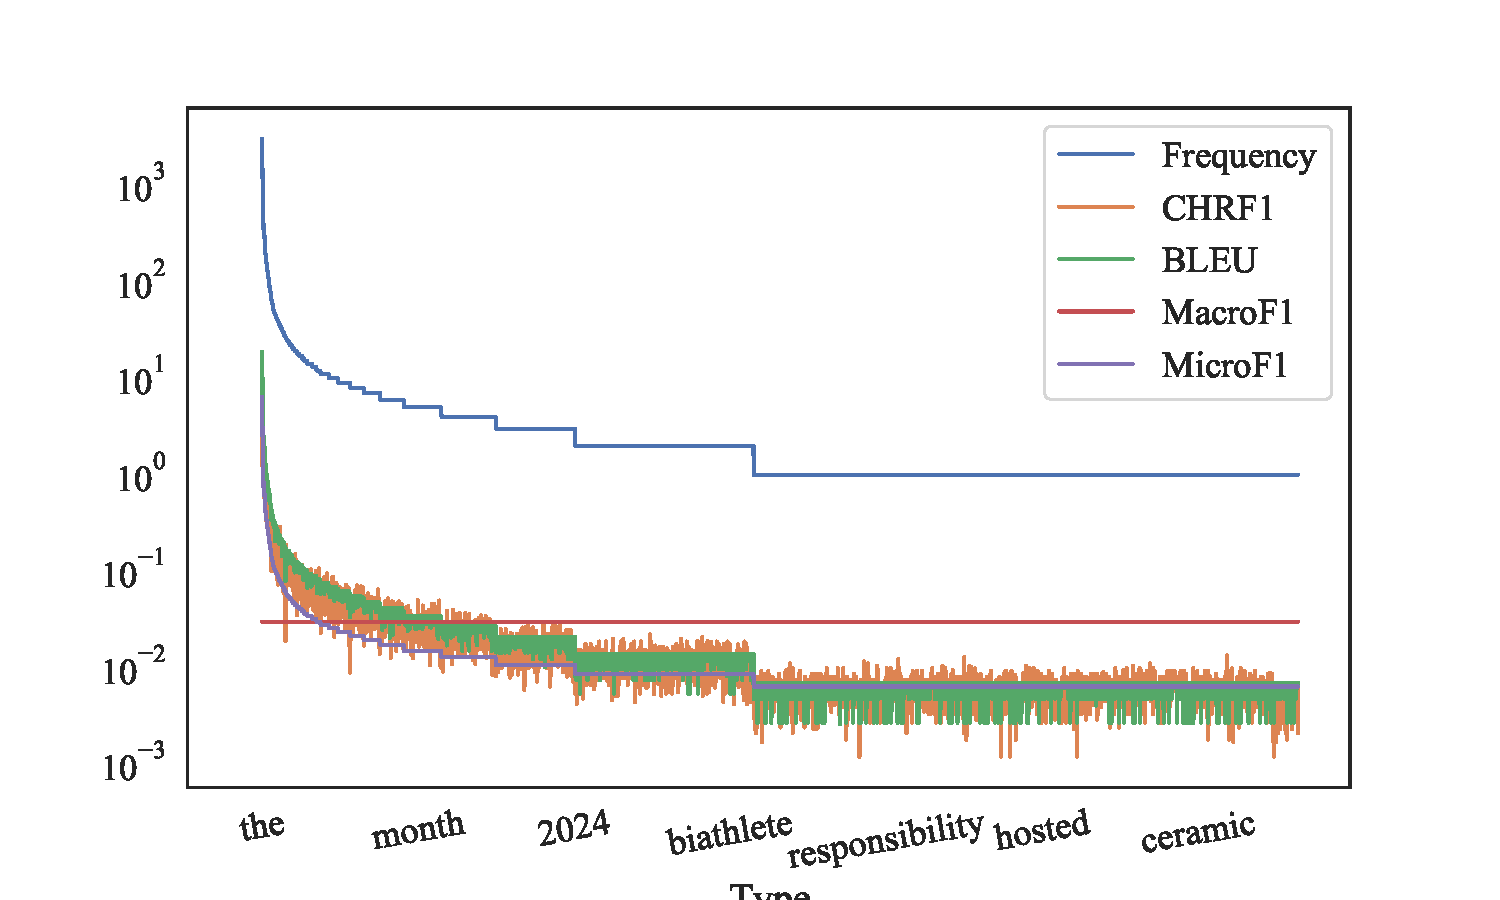
\includegraphics[width=\textwidth,trim={0mm 5mm 0mm 0mm},clip]{img/macroavg/bleu-chrf-macro-micro-swapin-lenmatch.pdf}
    \caption{MT metrics and their weights assigned to word types.
    Statistics are from WMT 2019 German-English NewsTest reference corpus.
    While \maf1{} treat each type equally, all others treat each token equally. }
    \label{fig:bleu-damage}
\end{figure}

\subsection{Data-to-Text: WebNLG}
\label{sec:webnlg}


\begin{table}[ht]
%    \footnotesize
    \centering
    \begin{tabular}{lrr}
Name & Fluency \& Grammar & Semantics \\ \hline\hline
\bleu\  & \insig.444 & \insig.500 \\
\chrf1 & \insig.278    & .778   \\
\maf1  & \insig.222    & .722   \\
\mif1  & \insig.333    & .611   \\ \hline
\blrtmn & \insig.444   & .833   \\
\blrtmd & .611  & .667   \\
\end{tabular}
    \caption{WebNLG data-to-text task: Kendall's $\tau$ between system-level MT metric scores and human judgments.
    Fluency and grammar are correlated identically by all metrics.
    Values that are \textit{not} significant at $\alpha=0.05$ are indicated by \insig{}.}
    \label{tab:webnlg-kendall}
\end{table}


We use the 2017 WebNLG Challenge dataset \cite{gardent2017webNLG-corpus, shimorina2018webnlg-human-eval}\footnote{\url{https://gitlab.com/webnlg/webnlg-human-evaluation}} to analyze the differences between micro- and macro- averaging. 
WebNLG is a task of generating English text for sets of triples extracted from DBPedia.
Human annotations are available for a sample of 223 records each from nine NLG systems.
The human judgments provided have three linguistic aspects---fluency, grammar, and semantics\footnote{Fluency and grammar, which are elicited with nearly identical directions \cite{gardent2017webNLG-corpus}, are identically correlated.}---which enable us to perform a fine-grained analysis of our metrics.
We compute Kendall's $\tau$ between metrics and human judgments, which are reported in Table~\ref{tab:webnlg-kendall}.

As seen in Table~\ref{tab:webnlg-kendall}, the metrics exhibit much variance in agreements with human judgments. %Fluency and grammar display same correlations and hence are com  
For instance, \blrtmd\ is the best indicator of fluency and grammar, however \blrtmn\ is best on semantics. 
BLEURT, being a \textit{model-based} measure that is directly trained on human judgments, scores relatively higher than others.
Considering the model-free metrics, \chrf1 does well on semantics but poorly on fluency and grammar compared to \bleu.
Not surprisingly, both \mif1 and \maf1, which rely solely on unigrams, are poor indicators of fluency and grammar compared to \bleu, however \maf1 is clearly a better indicator of semantics than \bleu. 
The discrepancy between \mif1 and \maf1 regarding their agreement with fluency, grammar, and semantics is expected: micro-averaging pays more attention to function words (as they are frequent types) that contribute to fluency and grammar whereas macro-averaging pays relatively more attention to the content words that contribute to semantic adequacy. 

The takeaway from this analysis is as follows: \maf1 is a strong indicator of semantic adequacy, however, it is a poor indicator of fluency. We recommend using either \maf1 or \chrf1 when semantic adequacy and not fluency is a desired goal.

\subsection{Machine Translation: WMT Metrics}
\label{sec:wmt-metrics}

\begin{table*}[ht!]
    %\footnotesize
    %\small
    \centering
    
\begin{tabular}{r r l r r r r r }
Year & Pairs  & & $\star$\bleu\ & \bleu\ & \maf1 & \mif1 & \chrf1 \\ \hline\hline
\multirow{3}{*}{ 2019 } 
    & \multirow{3}{*}{18}
     & Mean   & .751 & .771 & .821 & .818 & .841  \\ 
   & & Median & .782 & .752 & .844 & .844 & .875  \\
   & & Wins   &     3 &     3 &  \textbf{6}    &     3 &   5 \\ \hline
\multirow{3}{*}{ 2018 } 
  & \multirow{3}{*}{14}
   & Mean   & .858 & .857 & .875 & .873 & .902  \\ 
  & & Median & .868 & .868 & .901 & .879 & .919  \\
  & & Wins    &  1  &  2 & 3 &  2 &  \textbf{6}\\ \hline  
\multirow{3}{*}{ 2017 }
   & \multirow{3}{*}{13}
    & Mean   & .752 & .713 & .714 & .742 & .804 \\  
  & & Median & .758 & .733 & .735 & .728 & .791 \\
  & & Wins   & 5 & 4 & 2 & 2 & \textbf{6} \\
\end{tabular}   
\caption[WMT 2017--19 Metrics task: Mean and median Kendall's $\tau$ between MT metrics and human judgments.]{WMT 2017--19 Metrics task: Mean and median Kendall's $\tau$ between MT metrics and human judgments.
Correlations that are not significant at $\alpha=0.05$ are excluded from the calculation of mean, and median, and wins.
See Appendix Tables \ref{tab:wmt19-kendall}, \ref{tab:wmt18-kendall}, and \ref{tab:wmt17-kendall} for full details.
$\star$\bleu\ is pre-computed scores available in the metrics packages.
In 2018 and 2019, both \maf1 and \mif1 outperform \bleu, \maf1 outperforms \mif1.
\chrf1 has strongest mean and median agreements across the years.
Judging based on the number of wins, \maf1 has steady progress over the years, and outperforms others in 2019.
}
\label{tab:wmt-summary}
\end{table*}

In this section, we verify how well the metrics agree with human judgments using Workshop on Machine Translation (WMT) metrics task datasets for 2017--2019~\cite{WMT17-metrics,WMT18-metrics,WMT19-metrics-proceedings}.\footnote{\url{http://www.statmt.org/wmt19/metrics-task.html}}
We first compute scores from each MT metric, and then calculate the correlation $\tau$ with human judgments.

As there are many language pairs and translation directions in each year, we report only the mean and median of $\tau$, and number of wins per metric for each year in Table \ref{tab:wmt-summary}.
We have excluded BLEURT from comparison in this section since the BLEURT models are fine-tuned on the same datasets on which we are evaluating the other methods.\footnote{\url{https://github.com/google-research/bleurt}}
\chrf1 has the strongest mean and median agreement with human judgments across the years.
In 2018 and 2019, both \maf1 and \mif1 mean and median agreements outperform \bleu\, whereas in 2017 \bleu\ was better than \maf1 and \mif1.


As seen in Section~\ref{sec:webnlg}, \maf1 weighs towards semantics whereas \mif1 and \bleu\ weigh towards fluency and grammar.
This indicates that recent MT systems are mostly fluent, and adequacy is the key discriminating factor amongst them.
\bleu\ served well in the early era of statistical MT when fluency was a harder objective. 
Recent advancements in neural MT models such as Transformers \cite{vaswani-2017-attention} produce fluent outputs, and have brought us to an era where semantic adequacy is the focus.


% save it for the slides
%We envision that the methods such as \maf1 that emphasize the long tail be more successful in the future years, and this vision is inline with \citet{steedman-2008-last}:
%One day, either because of the demise of Moore’slaw, or simply because we have done all the easy stuff, the Long Tail will come back to haunt us.
%\textit{``One day, ... simply because we have done all the easy stuff, the Long Tail will come back to haunt us.''}


%\section{Agreement with WMT Human Judgments}
%\label{sec:apphuman}

Tables \ref{tab:wmt19-kendall}, \ref{tab:wmt18-kendall}, and \ref{tab:wmt17-kendall} provide $\tau$ between MT metrics and human judgments on WMT Metrics task 2017--2019. 
$\star$\bleu\ is based on pre-computed scores in WMT metrics package, whereas \bleu\ is based on our recalculation using \textsc{SacreBleu}. 
Values marked with \insig are not significant at $\alpha=0.05$, and hence corresponding rows are excluded from the calculation of mean, median, and standard deviation.

Since \maf1 is the only metric that does not achieve statistical significance in the WMT 2019 EN-ZH setting, we carefully inspected it.
Human scores for this setting are obtained without looking at the references by bilingual speakers \cite{WMT19-metrics-proceedings}, but the ZH references are found to have a large number of bracketed EN phrases, especially proper nouns that are rare types.
When the text inside these brackets is not generated by an MT system, \maf1 naturally penalizes heavily due to the poor recall.
Since other metrics assign lower importance to poor recall of such rare types, they achieve relatively better correlation to human scores than \maf1. 
However, since the $\tau$ values for EN-ZH are relatively lower than the other language pairs, we conclude that poor correlation of \maf1 in EN-ZH is due to poor quality references.
Some settings did not achieve statistical significance due to a smaller sample set as there were fewer MT systems submitted, e.g. 2017 CS-EN.

\begin{table}[ht!]
    %\footnotesize
\small 
\parbox{.48\linewidth}{
\centering
\begin{tabular}{l @{\hspace{1mm}} r @{\hspace{1mm}} r @{\hspace{1mm}} r @{\hspace{1mm}} r @{\hspace{1mm}} r}
 & $\star$\bleu & \bleu & \maf1 & \mif1 & \chrf1 \\ \hline \hline
DE-CS & .855 & .745 & .964 & .917 & \textbf{.982}  \\
DE-EN & .571 & .655 & .723 & .695 & \textbf{.742} \\
DE-FR & .782 & .881 & \textbf{.927} & .844 & .915 \\
EN-CS & .709 & \textbf{.954} & .927 & .927 & .908  \\
EN-DE & .540 & .752 & .741 & .773 & \textbf{.824} \\
EN-FI & .879 & .818 & .879 & .848 & \textbf{.923}  \\
EN-GU & .709 & .709 & .600 & \textbf{.734} & .709  \\
EN-KK & .491 & .527 & \textbf{.685} & .636 & .661  \\
EN-LT & .879 & .848 & \textbf{.970} & .939 & .881 \\
EN-RU & .870 & .848 & \textbf{.939} & .879 & .930  \\
FI-EN & .788 & .809 & \textbf{.909} & .901  & .875 \\
FR-DE & \textbf{.822} & .733 & .733 & .764  & .815 \\
GU-EN & .782 & .709 & .855 & .891 & \textbf{.945}  \\
KK-EN & \textbf{.891} & .844 & .796 & .844 & .881 \\
LT-EN & .818 & \textbf{.855} & .844 & \textbf{.855}  & .833 \\
RU-EN & .692 & .729 & .714 & \textbf{.780} & .757 \\
ZH-EN & .695 & .695 & \textbf{.752} & .676 & .715 \\ \hline
Median & .782 & .752 & .844 & .844 & .875\\
Mean & .751 & .771 & .821 & .818 & .841  \\
SD & .124 & .101 & .112 & .093 & .095  \\ \hline
EN-ZH & \textbf{.606} & \textbf{.606} & \insig.424 & .595 & .594 \\ \hline
Wins & 3 & 3 & 6 & 3 & 5 
\end{tabular} 
\caption{ WMT19 Metrics task: Kendall's $\tau$ between metrics and human judgments.}
\label{tab:wmt19-kendall}
}
\hfill
%\end{table}
%\vspace{2px}
%\begin{table}[ht]
    %\footnotesize
\parbox{.48\linewidth}{
%    \centering
\begin{tabular}{l @{\hspace{1mm}} r @{\hspace{1mm}} r @{\hspace{1mm}} r @{\hspace{1mm}} r @{\hspace{1mm}} r}
 & $\star$\bleu & \bleu & \maf1 & \mif1 & \chrf1 \\ \hline \hline
DE-EN & .828 & .845 & .917 & .883 & \textbf{.919}  \\
EN-DE & .778 & .750 & \textbf{.850} & .783 & .848  \\
EN-ET & .868 & .868 & .934 & .906 & \textbf{.949}  \\
EN-FI & .901 & .848 & .901 & .879 & \textbf{.945}  \\
EN-RU & .889 & .889 & \textbf{.944} & .889 & .930  \\
EN-ZH & .736 & .729 & .685 & \textbf{.833} & .827 \\
ET-EN & .884 & .900 & .884 & .878 & \textbf{.904}  \\
FI-EN & .944 & .944 & .889 & .915 & \textbf{.957}  \\
RU-EN & .786 & .786 & \textbf{.929} & .857 & .869 \\
ZH-EN & .824 & \textbf{.872} & .738 & .780 & .820  \\ 
EN-CS & \textbf{1.000} & \textbf{1.000} & .949 & \textbf{1.000} & .949  \\ \hline

Median & .868 & .868 & .901 & .879 & .919  \\
Mean   & .858 & .857 & .875 & .873 & .902  \\
SD     & .077 & .080 & .087 & .062 & .052  \\ \hline

TR-EN & \insig.200 & \insig.738 & \insig.400 & \insig.316 & \insig.632 \\
EN-TR & \insig.571 & \insig.400 & .837 & \insig.571 & \textbf{.849}  \\
CS-EN & \insig.800 & \insig.800 & \insig.600 & \insig.800 & \insig.738 \\ \hline
Wins &  1  &  2 & 3 &  2 & 6
\end{tabular}
\caption{ WMT18 Metrics task: Kendall's $\tau$ between metrics and human judgments.}
\label{tab:wmt18-kendall}
}
\end{table}


%\vspace{2px}
\begin{table}[ht]
    %\footnotesize
    \centering
\begin{tabular}{l @{\hspace{1.5mm}} r @{\hspace{1.5mm}} r @{\hspace{1.5mm}} r @{\hspace{1.5mm}} r @{\hspace{1.5mm}} r}
 & $\star$\bleu & \bleu & \maf1 & \mif1 & \chrf1 \\ \hline \hline
DE-EN & .564 & .564 & .734 & .661 & \textbf{.744}  \\
EN-CS & .758 & .751 & .767 & .758 & \textbf{.878} \\
EN-DE & .714 & \textbf{.767} & .562 & .593 & .720  \\
EN-FI & .667 & .697 & .769 & .718 & \textbf{.782} \\
EN-RU & .556 & .556 & \textbf{.778} & .648 & .669  \\
EN-ZH & \textbf{.911} & \textbf{.911} & .600 & .854 & .899 \\
LV-EN & \textbf{.905} & .714 & \textbf{.905} & \textbf{.905} & \textbf{.905}  \\
RU-EN & .778 & .611 & .611 & .722 & \textbf{.800}  \\
TR-EN & \textbf{.911} & .778 & .674 & .733 & .907  \\
ZH-EN & .758 & \textbf{.780} & .736 & .824 & .732  \\ \hline
Median & .758 & .733 & .735 & .728 & .791 \\
Mean & .752 & .713 & .714 & .742 & .804  \\
SD & .132 & .110 & .103 & .097 & .088  \\ \hline
FI-EN & \textbf{.867} & \textbf{.867} & \insig.733 & \textbf{.867} & \textbf{.867} \\
EN-TR & \textbf{.857} & .714 & \insig.571 & .643 & .849 \\
CS-EN & \insig1.000 & \insig1.000 & \insig.667 & \insig.667 & \insig.913 \\  \hline
Wins & 5 & 4 & 2 & 2 & 6
\end{tabular} 
\caption{ WMT17 Metrics task: Kendall's $\tau$ between metrics and human judgments.}
\label{tab:wmt17-kendall}
\end{table}



\subsection{Downstream Task: Cross-Lingual Information Retrieval}
\label{sec:clir}
In this section, we determine correlation between MT metrics and  downstream cross-lingual information retrieval (CLIR) tasks.
CLIR is a kind of information retrieval (IR) task in which documents in one language are retrieved given queries in another~\cite{grefenstette2012CLIR}. 
A practical solution to CLIR is to translate source documents into the query language using an MT model, then use a monolingual IR system to match queries with translated documents. 
Correlation between MT and IR metrics is accomplished in the following steps: 
\begin{enumerate}[noitemsep,topsep=0pt]
 \item Build a set of MT models and measure their performance using MT metrics.
 \item Using each MT model in the set, translate all source documents to the target language, build an IR model, and measure IR performance on translated documents.
 \item For each MT metric, find the correlation between the set of MT scores and their corresponding set of IR scores.
 The MT metric that has a stronger correlation with the IR metric(s) is more useful than the ones with weaker correlations.
\item Repeat the above steps on many languages to verify the generalizability of findings.
\end{enumerate}


An essential resource for this analysis is a dataset with human annotations for computing MT and IR performances.
We conduct experiments on two datasets: firstly, on data from the 2020 workshop on \textit{Cross-Language Search and Summarization of Text and Speech} (CLSSTS) \cite{zavorin-etal-2020-corpora}, and secondly, on data originally from Europarl, prepared by \citet{lignos-etal-2019-MT-IR} (Europarl).

\subsubsection{CLSSTS Datasets}
\label{sec:material}

\begin{table*}[ht]
    %\footnotesize
    \small 
    \begin{tabular}{l l l r r r r r r }
 & Domain & IR Score & \bleu\ & \maf1 & \mif1 & \chrf1 & {\footnotesize \blrtmn} & {\footnotesize \blrtmd} \\\hline\hline

\multirow{4}{*}{LT-EN} 
& \multirow{2}{*}{In} 
  & AQWV & .429 & \insig.363 & \textbf{.508} & \insig.385 & .451  & .420 \\
& & MAP  & .495  & .429      & \textbf{.575} & .451       & .473  & .486 \\
& \multirow{2}{*}{In+Ext}
   & AQWV & \insig.345 & \textbf{.527} & .491  & .491 & .491 & .477 \\
&  & MAP  & \insig.273 & \insig\textbf{.455} & \insig.418 & \insig.418 & \insig.418 & \insig.404 \\\hline
\multirow{4}{*}{PS-EN}
  & \multirow{2}{*}{In} 
    & AQWV  & .559 & \textbf{.653} & .574 & .581 & .584 & .581  \\
  & & MAP   & .493 & \textbf{.632} & .487 & .494 & .558 & .554 \\
  & \multirow{2}{*}{In+Ext}
    & AQWV   & .589 & \textbf{.682} & .593 & .583 & .581 & .571 \\
  & & MAP    & .519 & \textbf{.637} & .523 & .482 & .536 & .526 \\\hline
\multirow{4}{*}{BG-EN}
 & \multirow{2}{*}{In} 
    & AQWV   & \insig.455 & \textbf{.550}   & .527  & \insig.382 & \insig.418  & .418 \\ 
 &  & MAP    &  .491      &  \textbf{.661}  & .564  &  .491       & .527       & .527 \\ 
 & \multirow{2}{*}{In+ext}
    & AQWV   & \insig.257 & \textbf{.500}       & \insig.330 & \insig.404 & \insig.367 & \insig.367 \\
 &  & MAP   & \insig.183 & \insig\textbf{.426} & \insig.257 & \insig.330 & \insig.294 & \insig.294 
\end{tabular} 
\caption{CLSSTS CLIR task: Kendall's $\tau$ between IR and MT metrics under study.
The rows with Domain=In are where MT and IR scores are computed on the same set of documents, whereas Domain=In+Ext are where IR scores are computed on a larger set of documents that is a superset of segments on which MT scores are computed.
\textbf{Bold} values are the best correlations achieved in a row-wise setting; values with \insig~ are \textit{not} significant at $\alpha=0.05$.}
\label{tab:material-kendall}
\end{table*}


CLSSTS datasets contain queries in English~(EN), and documents in many source languages along with their human translations, as well as query-document relevance judgments. 
We use three source languages: Lithuanian~(LT), Pashto~(PS), and Bulgarian~(BG).
The performance of this CLIR task is evaluated using two IR measures: Actual Query Weighted Value (AQWV) and Mean Average Precision (MAP).
AQWV\footnote{\href{https://www.nist.gov/system/files/documents/2017/10/26/aqwv\_derivation.pdf}{https://www.nist.gov/system/files/documents-/2017/10/26/aqwv\_derivation.pdf}} is derived from Actual Term Weighted Value (ATWV) metric \cite{wegmann2013ATWV}. 
We use a single CLIR system \cite{boschee-etal-2019-saral} with the same IR settings for all MT models in the set, and measure Kendall's $\tau$ between MT and IR measures.
The results, in Table~\ref{tab:material-kendall}, show that \maf1 is the strongest indicator of CLIR downstream task performance in five out of six settings.
AQWV and MAP have a similar trend in agreement to the MT metrics.
\chrf1 and BLEURT, which are strong contenders when generated text is directly evaluated by humans, do not indicate CLIR task performance as well as \maf1, as CLIR tasks require faithful meaning equivalence across the language boundary, and human translators can mistake fluent output for proper translations \cite{callison-burch-etal-2007-meta}. 


\subsubsection{Europarl Datasets}
\label{sec:lignos-etal}

\begin{table}[ht]
    %\footnotesize
    \centering
    %\setlength{\tabcolsep}{10pt}
\begin{tabular}{l r r r r r r}
 & \bleu\ & \maf1 & \mif1 & \chrf1 & \blrtmn & \blrtmd \\ \hline\hline
\multirow{1}{*}{ CS-EN } 
 & .850 & .867 & .850 & .850 & \textbf{.900} & .867 \\ 
\multirow{1}{*}{ DE-EN } 
  & .900 & .900 & .900 & .912 & \textbf{.917} & .900 \\
\end{tabular}  
\caption{Europarl CLIR task: Kendall's $\tau$ between MT metrics and RBO. All correlations are significant at $\alpha=0.05$.}
\label{tab:lignos-mtir-kendall} 
\end{table}


We perform a similar analysis to Section \ref{sec:material} but on another cross-lingual task set up by \citet{lignos-etal-2019-MT-IR} for Czech $\rightarrow$ English (CS-EN) and German $\rightarrow$ English (DE-EN), using publicly available data from the Europarl v7 corpus~\cite{koehn2005europarl}. 
This task differs from the CLSSTS task (Section \ref{sec:material}) in several ways.
Firstly, MT metrics are computed on test sets from the news domain, whereas IR metrics are from the Europarl domain. The domains are thus intentionally mismatched between MT and IR tests.
Secondly, since there are no queries specifically created for the Europarl domain, GOV2 TREC topics 701–850 are used as domain-relevant English queries.
And lastly, since there are no query-document relevance human judgments for the chosen query and document sets, the documents retrieved by BM25~\cite{jones2000probabilistic} on the English set for each query are treated as relevant documents for computing the performance of the CS-EN and DE-EN CLIR setup. 
As a result, IR metrics that rely on boolean query-document relevance judgments as ground truth are less informative, and we use Rank-Based Overlap (RBO; $p=0.98$) \cite{webber2010RBO} as our IR metric.

We perform our analysis on the same experiments as \citet{lignos-etal-2019-MT-IR}.\footnote{\url{https://github.com/ConstantineLignos/mt-clir-emnlp-2019}}
NMT models for CS-EN and DE-EN translation are trained using a convolutional NMT architecture \cite{gehring2017CNNMT} implemented in the FAIRSeq~\cite{ott-etal-2019-fairseq} toolkit.
For each of CS-EN and DE-EN, a total of 16 NMT models that are based on different quantities of training data and BPE hyperparameter values are used.
The results in Table~\ref{tab:lignos-mtir-kendall} show that BLEURT has the highest correlation in both cases.
Apart from the trained \blrtmd\ metric, \maf1 scores higher than the others on CS-EN, and is competitive on CS-EN. \maf1 is not the metric with the highest IR task correlation in this setting, unlike in Section \ref{sec:material}, however it is competitive with \bleu\ and \chrf1, and thus a safe choice as a downstream task performance indicator. 


\section{Spotting Differences Between Supervised and Unsupervised NMT}
\label{sec:unmt}

Unsupervised neural machine translation (UNMT) systems trained on massive monolingual data without parallel corpora have made significant progress recently \cite{Artetxe-2018-unmt-iclr,Lample-2018-unmt-iclr,lample-etal-2018-phrase-unmt,conneau-NIPS2019-xlm,Song-2019-MASS,liu-etal-2020-multilingual-denoising}. 
In some cases, UNMT yields a \bleu\ score that is comparable with strong\footnote{though not, generally, the strongest} supervised neural machine translation (SNMT) systems. In this section we leverage \maf1 to investigate differences in the translations from UNMT and SNMT systems that have similar \bleu.

We compare UNMT and SNMT for English $\leftrightarrow$ German (EN-DE, DE-EN), English $\leftrightarrow$ French (EN-FR, FR-EN), and English $\leftrightarrow$ Romanian (EN-RO, RO-EN).
All our UNMT models are based on XLM \citep{conneau-NIPS2019-xlm}, pretrained by \citet{XLM-UNMT-Models20}. 
We choose SNMT models with similar \bleu\ on common test sets by either selecting from systems submitted to previous WMT News Translation shared tasks~\cite{bojar-etal-2014-findings,bojar-etal-2016-findings} or by building such systems.\footnote{We were unable to find EN-DE and DE-EN systems with comparable \bleu\ in WMT submissions so we built standard Transformer-base~\cite{vaswani-2017-attention} models for these using appropriate quantity of training data to reach the desired \bleu\ performance. We report EN-RO results with diacritic removed to match the output of UNMT.} Specific SNMT models chosen are in Table~\ref{tab:unmt_vs_snmt2}. 
The UNMT models follow XLM's standard architecture and are trained with 5 million monolingual sentences for each language using a vocabulary size of 60,000. 
% using code base from \citet{rtg-xt20}
We train SNMT models for EN$\leftrightarrow$DE and select models with the most similar (or a slightly lower) BLEU as their UNMT counterparts on newstest2019. The DE-EN model selected is trained with 1 million sentences of parallel data and a vocabulary size of 64,000, and the EN-DE model selected is trained with 250,000 sentences of parallel data and a vocabulary size of 48,000. For EN$\leftrightarrow$FR and EN$\leftrightarrow$RO, we select SNMT models from submitted systems to WMT shared tasks that have similar or slightly lower BLEU scores to corresponding UNMT models, based on \textit{NewsTest2014} for EN$\leftrightarrow$FR and \textit{NewsTest2016} for EN$\leftrightarrow$RO. 

%\subsection{UNMT and SNMT Models}
\begin{table}[ht!]
% \resizebox{\textwidth}{!}{%
\centering
%\footnotesize
\begin{tabular}{l @{\hspace{1.5mm}} r @{\hspace{1.5mm}} r @{\hspace{1.5mm}} l}
Translation & SNMT    & UNMT  &  SNMT Name      \\ \hline \hline
DE-EN NewsTest2019     & 32.7   & 33.9  & \textit{Our Transformer}             \\
EN-DE NewsTest2019     & 24.0   & 24.0  & \textit{Our Transformer}           \\
FR-EN NewsTest2014     & 31.1   & 31.2  & OnlineA.0             \\
EN-FR NewsTest2014     & 25.6   & 27.1  & PROMT-Rule-based.3083 \\
RO-EN NewsTest2016     & 30.8   & 29.6  & Online-A.0            \\
EN-RO NewsTest2016     & 31.2   & 31.0  & uedin-pbmt.4362      \\ 
\end{tabular}%
% }
\caption{ We select SNMT systems such that their \bleu\ scores are approximately the same as the available pretrained UNMT models. \textit{Our Transformer} models are the ones we have trained, which are described in  Chapter~\ref{ch:nlg-imbalance}.} 
\label{tab:unmt_vs_snmt2}
\end{table}


\begin{table*}[ht!]
\centering
\small
\setlength{\tabcolsep}{4pt}
%\footnotesize
\begin{tabular}{l @{\hspace{3mm}} r @{\hspace{1.5mm}} r @{\hspace{1.5mm}}r :  r@{\hspace{1.5mm}}r@{\hspace{1.5mm}}r :
  r@{\hspace{1.5mm}}r@{\hspace{1.5mm}}r : r@{\hspace{1.5mm}} r@{\hspace{1.5mm}} r : r@{\hspace{1.5mm}} r@{\hspace{1.5mm}} r : r @{\hspace{1.5mm}} r@{\hspace{1.5mm}} r}
& \multicolumn{3}{c:}{\bleu} & \multicolumn{3}{c:}{ \maf1 } & \multicolumn{3}{c:}{ \mif1 } & \multicolumn{3}{c:}{ \chrf1 } & \multicolumn{3}{c:}{ \blrtmn } & \multicolumn{3}{c}{ \blrtmd } \\ 
& SN & UN & $\Delta$ & SN & UN & $\Delta$ & SN & UN & $\Delta$ & SN & UN & $\Delta$ & SN & UN & $\Delta$ & SN & UN & $\Delta$ \\ \hline \hline
DE-EN & 32.7 & 33.9 & -1.2 & 38.5 & 33.6 & 4.9 & 58.7 & 57.9 &  0.8 & 59.9 & 58.0 &  1.9 & .211 & -.026 & .24 & .285 & .067 & .22 \\
EN-DE & 24.0 & 24.0 &  0.0 & 24.0 & 23.5 & 0.5 & 47.7 & 48.1 & -0.4 & 53.3 & 52.0 &  1.3 &-.134 & -.204 & .07 &-.112 &-.197 & .09 \\
FR-EN & 31.1 & 31.2 & -0.1 & 41.6 & 33.6 & 8.0 & 60.5 & 58.3 &  2.2 & 59.1 & 57.3 &  1.8 & .182 &  .066 & .17 & .243 & .154 & .09 \\
EN-FR & 25.6 & 27.1 & -1.5 & 31.9 & 27.3 & 4.6 & 53.0 & 52.3 &  0.7 & 56.0 & 57.7 & -1.7 & .104 &  .042 & .06 & .096 & .063 & .03 \\
RO-EN & 30.8 & 29.6 &  1.2 & 40.3 & 33.0 & 7.3 & 59.8 & 56.5 &  3.3 & 58.0 & 54.7 &  3.3 & .004 & -.058 & .06 & .045 & -.004 & .04 \\
EN-RO & 31.2 & 31.0 &  0.2 & 34.6 & 31.0 & 3.6 & 55.4 & 53.4 &  2.0 & 59.3 & 56.7 &  2.6 & .030 & -.046 & .08 & .027 & -.038 & .07 \\
\end{tabular} 

\caption{For each language direction, UNMT (UN) models have similar \bleu\ to SNMT (SN) models, and \chrf1 and \mif1 have small differences. 
However, \maf1 scores differ significantly, consistently in favor of SNMT. Both corpus-level interpretations of BLEURT support the trend reflected by \maf1, but the value differences are difficult to interpret. Credits: Weiqiu You.
}
\label{tab:unmt_vs_snmt}
\end{table*}


 Table~\ref{tab:unmt_vs_snmt} shows performance for these three language pairs using a variety of metrics. Despite comparable scores in \bleu\ and only minor differences in \mif1 and \chrf1, SNMT models have consistently higher \maf1 and BLEURT than the UNMT models for all six translation directions. 
 
 
 Figure~\ref{fig:snmt_vs_unmt}, which is a visualization of \maf1 for SNMT and UNMT models,  shows that UNMT is generally better than SNMT on frequent types, however, SNMT outperforms UNMT on the rest leading to a crossover point in \maf1 curves. 
Since \maf1 assigns relatively higher weights to infrequent types than in \bleu{}, SNMT gains higher \maf1 than UNMT while both have approximately the same \bleu{}, as reported in Table~\ref{tab:unmt_vs_snmt}.

\begin{figure}[ht!]
    \centering
    \begin{subfigure}[b]{0.495\linewidth}
    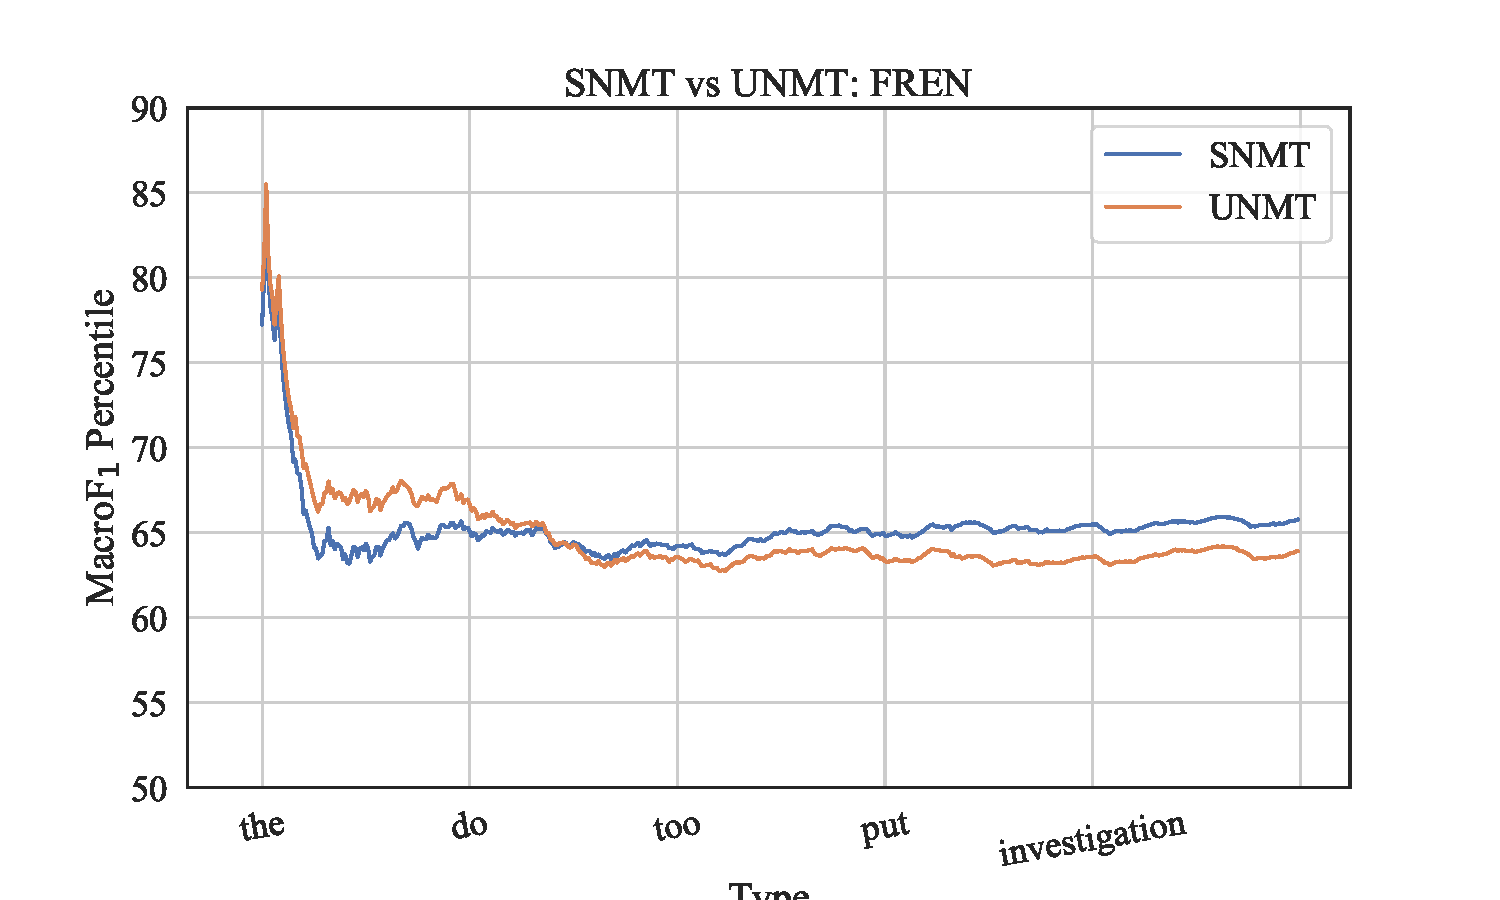
\includegraphics[width=\linewidth,trim={13mm 5mm 25mm 10mm},clip]{macroavg/s_unmt-fren-maf1.pdf}
    \end{subfigure}
    \begin{subfigure}[b]{0.495\linewidth}
    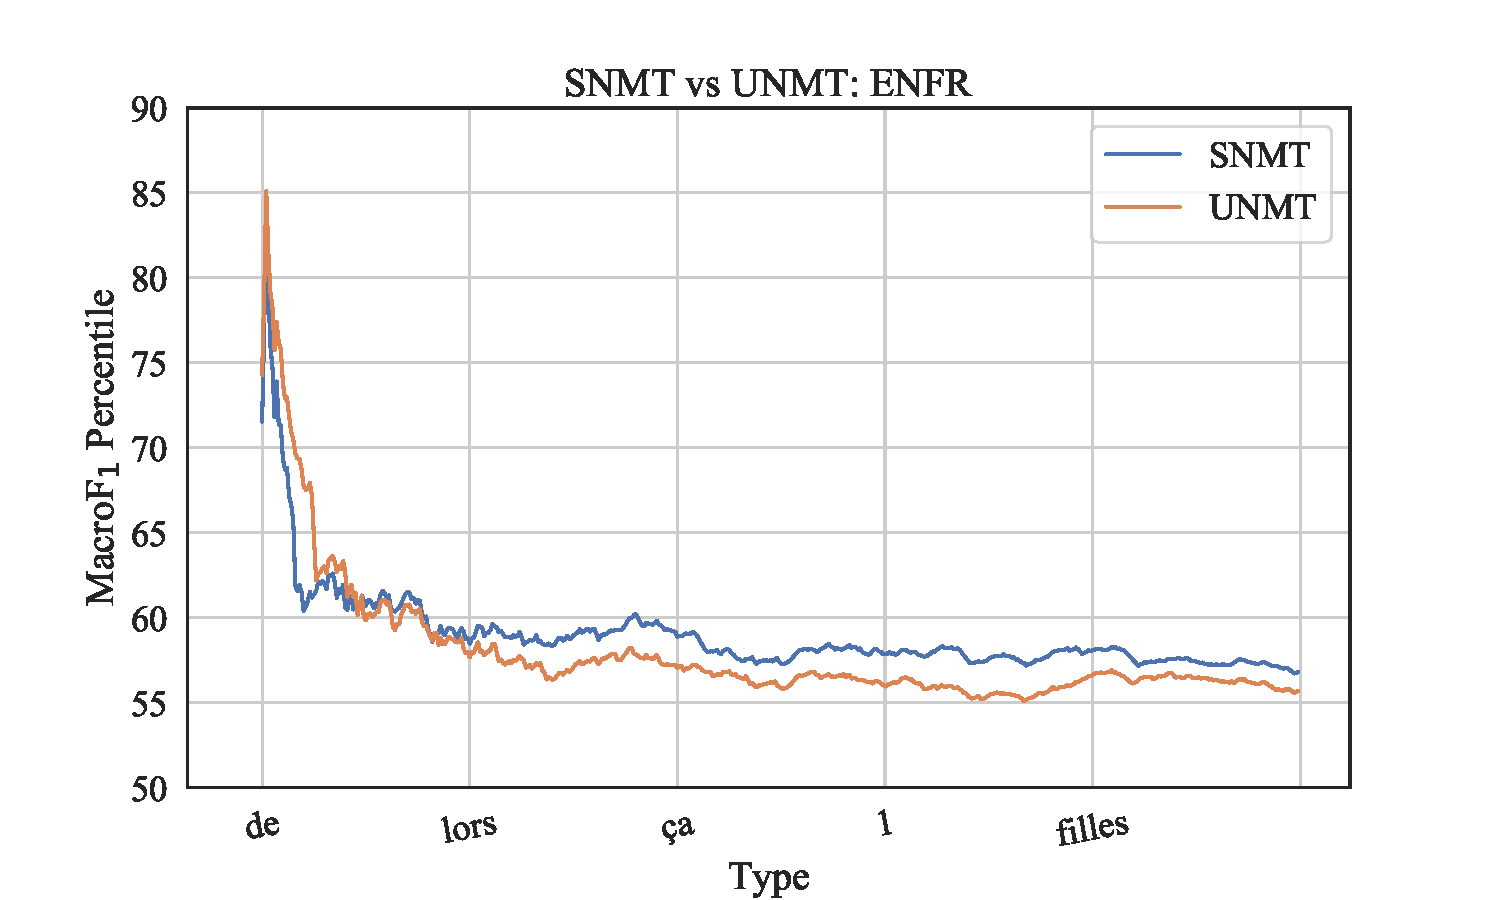
\includegraphics[width=\linewidth,trim={13mm 7mm 25mm 10mm},clip]{macroavg/s_unmt-enfr-maf1.pdf}
    \end{subfigure}
    
    \begin{subfigure}[b]{0.495\linewidth}
    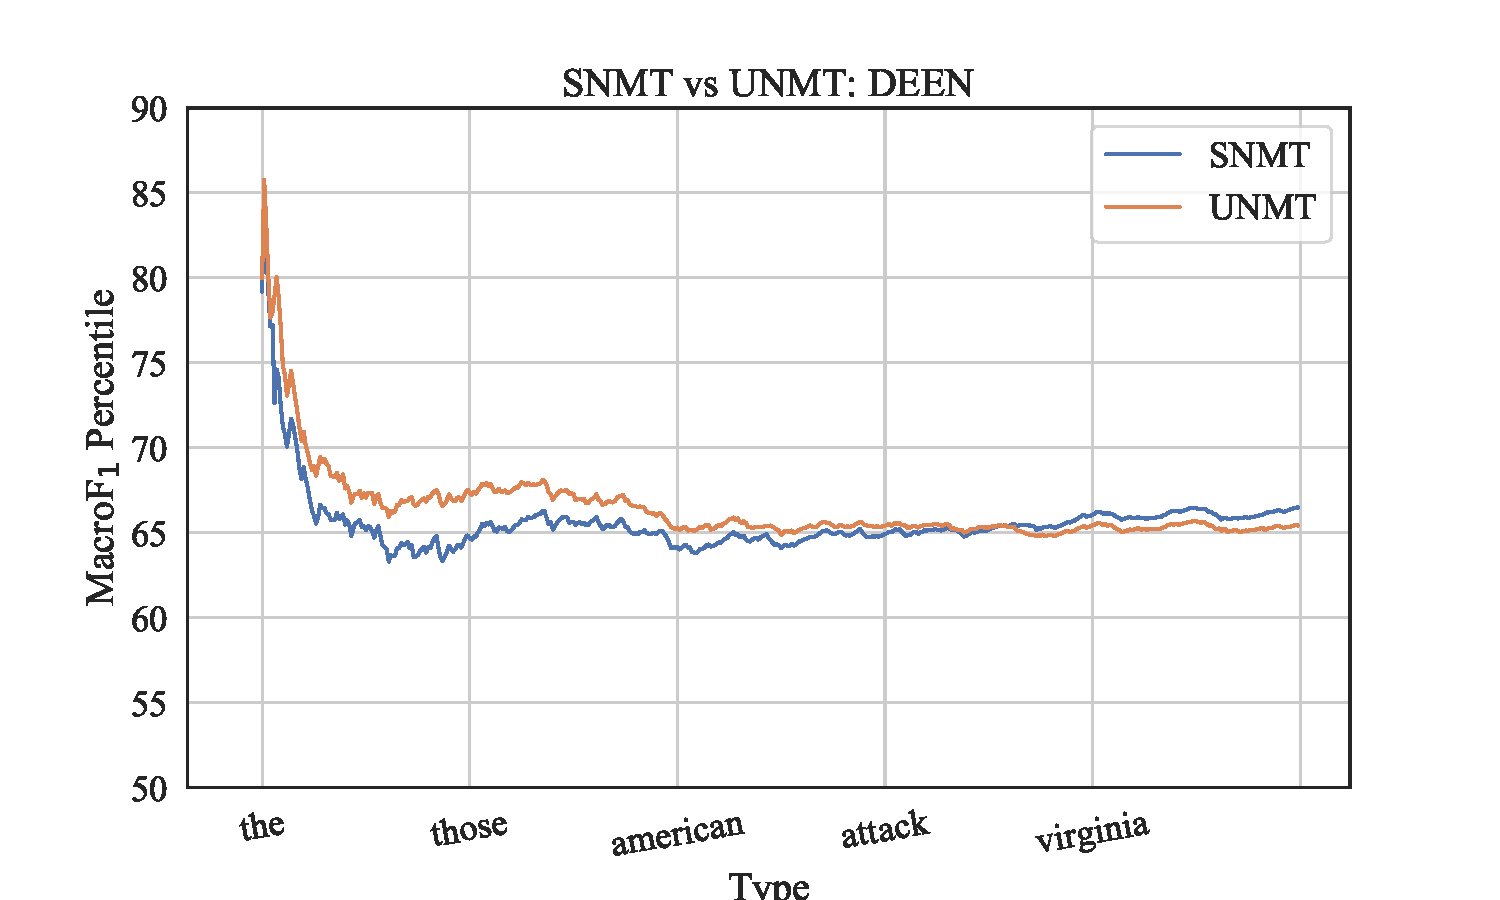
\includegraphics[width=\linewidth,trim={13mm 5mm 25mm 10mm},clip]{macroavg/s_unmt-deen-maf1.pdf}
    \end{subfigure}
    \begin{subfigure}[b]{0.495\linewidth}
    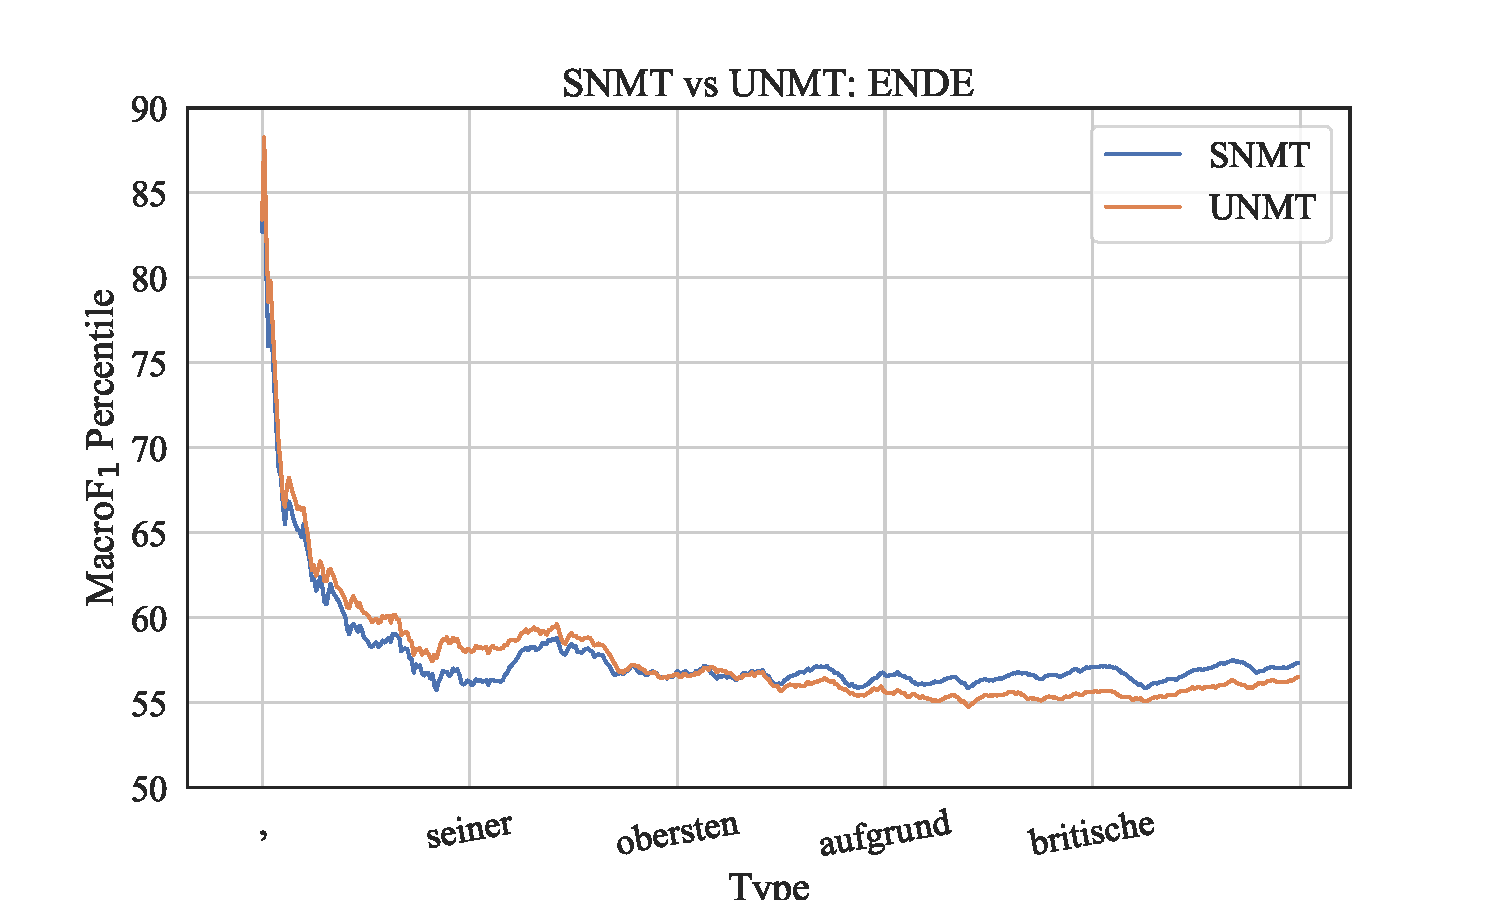
\includegraphics[width=\linewidth,trim={13mm 7mm 25mm 10mm},clip]{macroavg/s_unmt-ende-maf1.pdf}
    \end{subfigure}
    
    \begin{subfigure}[b]{0.495\linewidth}
    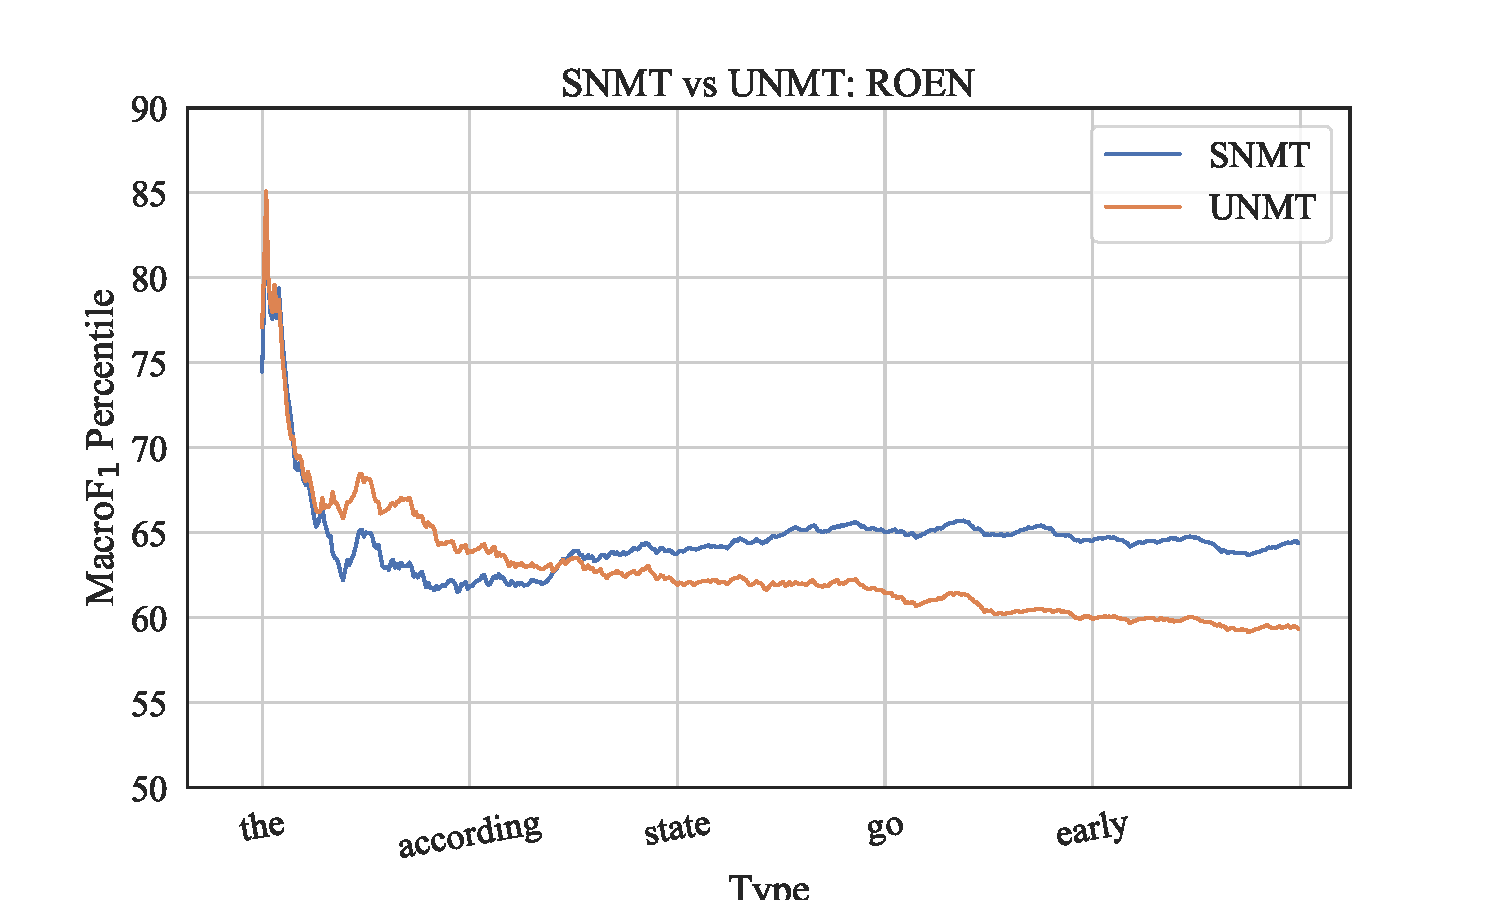
\includegraphics[width=\linewidth,trim={13mm 5mm 25mm 10mm},clip]{macroavg/s_unmt-roen-maf1.pdf}
    \end{subfigure}
    \begin{subfigure}[b]{0.495\linewidth}
      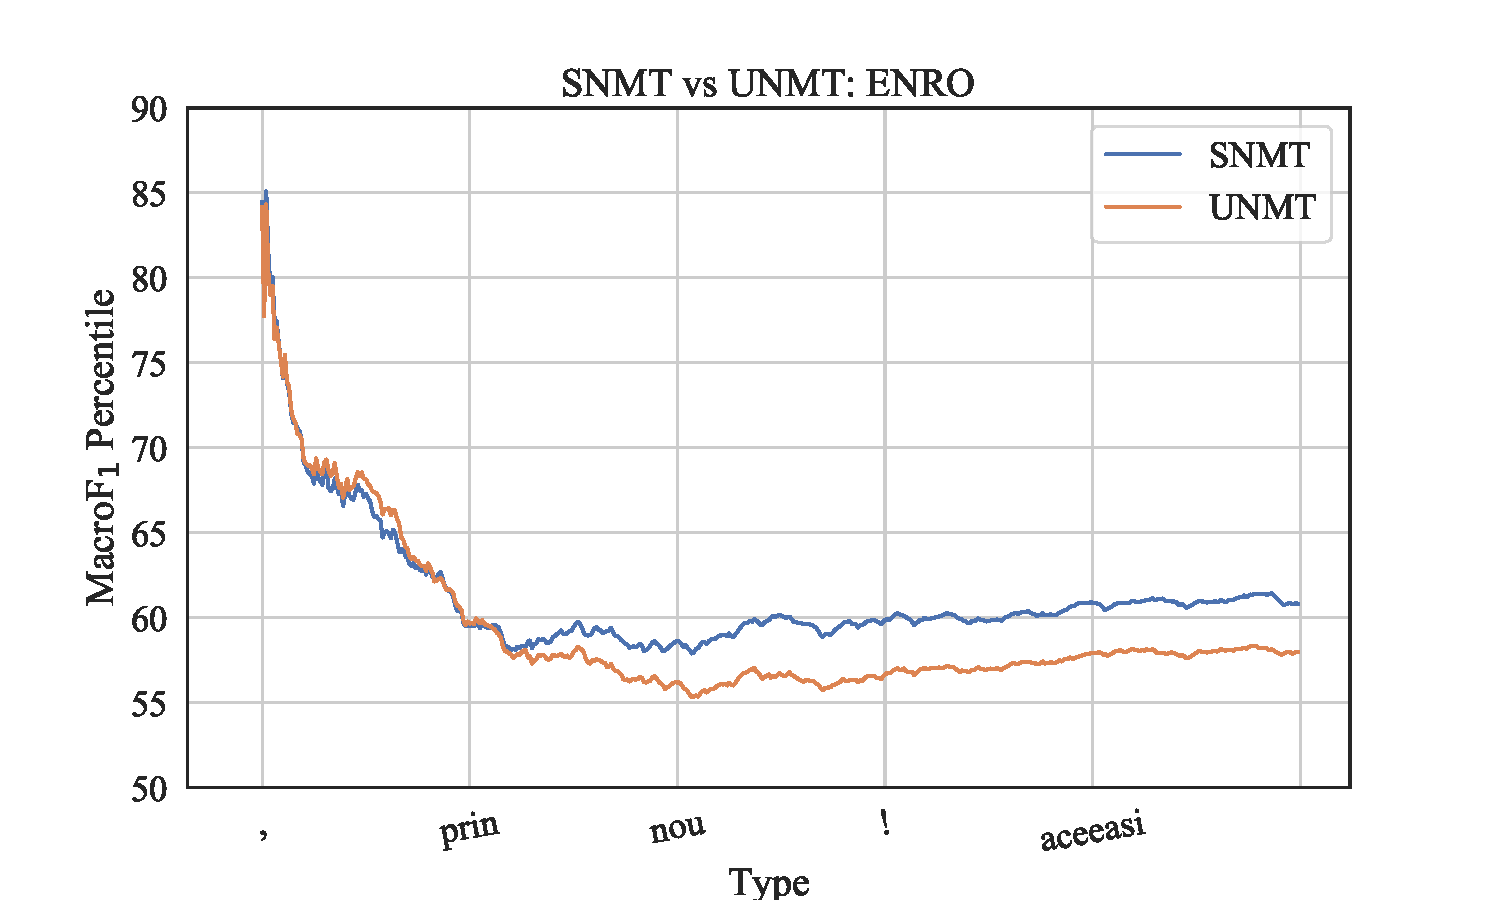
\includegraphics[width=\linewidth,trim={13mm 7mm 25mm 10mm},clip]{macroavg/s_unmt-enro-maf1.pdf}
      %\label{fig:snmt_vs_unmt_rest}
      %\caption{(Continued from Figure~\ref{fig:snmt_vs_unmt}) Visualization of \maf1 between SNMT and UNMT .  }
    \end{subfigure}
     
\caption{SNMT vs UNMT \maf1 on the most frequent 500 types.
UNMT outperforms SNMT on frequent types that are weighed heavily by \bleu\, however, SNMT is generally better than UNMT on rare types; hence, SNMT has a higher \maf1.
Only the most frequent 500 types are visualized in this figure.
}
\label{fig:snmt_vs_unmt}
\end{figure} 



%%%%%%% Appendix %%%%%%%%%%
\section{Metrics Reproducibility}
\label{sec:appmetrics}

\bleu\ scores reported in this work are computed with the \textsc{SacreBleu} library and have signature \texttt{\small BLEU+case.mixed+lang.<xx>-<yy>+numrefs.1+smooth.exp+tok.<TOK>+version.1.4.13}, where \texttt{<TOK>} is \texttt{zh} for Chinese, and \texttt{13a} for all other languages. \maf1 and \mif1 use the same tokenizer as \bleu.
\chrf1 is also obtained using \textsc{SacreBleu} and has signature \texttt{\small chrF1+lang.<xx>-<yy>+numchars.6 +space.false +version.1.4.13}.
BLUERT scores are from the \textit{base} model of \citet{sellam-etal-2020-bleurt}, which is fine-tuned on WMT Metrics ratings data from 2015-2018.
The BLEURT model is retrieved from \url{https://storage.googleapis.com/bleurt-oss/bleurt-base-128.zip}.

\maf1 and \mif1 are computed using our fork of \textsc{SacreBleu} as:\\
\texttt{sacrebleu \$REF -m macrof microf < \$HYP}. 
Our modification to SacreBLEU is available at \url{https://github.com/isi-nlp/sacrebleu/tree/macroavg-naacl21}; alternatively, it can be installed as \code{pip install sacrebleu-macrof}\footnote{\url{https://pypi.org/project/sacrebleu-macrof/2.0.1/}}

\section{Conclusion}
We have evaluated NLG in general and MT specifically as a multi-class classifier, and illustrated the differences between micro- and macro- averages using \mif1 and \maf1 as examples (Section~\ref{sec:mt-as-cls}).
\maf1 captures semantic adequacy better than \mif1 (Section~\ref{sec:webnlg}).
\bleu, being a micro-averaged measure, served well in an era when generating fluent text was at least as difficult as generating adequate text. Since we are now in an era in which fluency is taken for granted and semantic adequacy is a key discriminating factor, macro-averaged measures such as \maf1 are better at judging the generation quality of MT models (Section~\ref{sec:wmt-metrics}).
We have found that another popular metric, \chrf1, also performs well on direct assessment,
however, being an implicitly micro-averaged measure, it does not perform as well as \maf1 on downstream CLIR tasks (Section~\ref{sec:material}).
Unlike BLEURT, which is also adequacy-oriented, \maf1 is directly interpretable, does not require retuning on expensive human evaluations when changing language or domain, and does not appear to have uncontrollable biases resulting from data effects.
It is both easy to understand and to calculate, and is  
inspectable, enabling fine-grained analysis at the level of individual word types. These attributes make it a useful metric for understanding and addressing the flaws of current models. For instance, we have used \maf1 to compare supervised and unsupervised NMT models at the same operating point measured in \bleu, and determined that supervised models have better adequacy than the current unsupervised models (Section~\ref{sec:unmt}).

Macro-average is a useful technique for addressing the importance of the long tail of language, and \maf1 is our first step in that direction; we anticipate the development of more advanced macro-averaged metrics that take advantage of higher-order and character n-grams in the future. 


%\section*{Acknowledgements}
%The authors thank Shantanu Agarwal, Joel Barry, and Scott Miller for their help with CLSSTS CLIR experiments, and Daniel Cohen for discussions on IR evaluation methods. This research is based upon work supported by the Office of the Director of National Intelligence (ODNI), Intelligence Advanced Research Projects Activity (IARPA), via AFRL Contract FA8650-17-C-9116.  The views and conclusions contained herein are those of the authors and should not be interpreted as necessarily representing the official policies or endorsements, either expressed or implied, of the ODNI, IARPA, or the U.S. Government. The U.S. Government is authorized to reproduce and distribute reprints for Governmental purposes notwithstanding any copyright annotation thereon.


\section*{Ethical Consideration}
Since many ML models including NMT are themselves opaque and known to possess data-induced biases~\cite{prates2019-mt-bias}, using opaque and biased evaluation metrics in concurrence makes it even harder to discover and address the flaws in modeling.
Hence, we have raised concerns about the opaque nature of the current model-based evaluation metrics, and demonstrated examples displaying unwelcome biases in evaluation. We advocate the use of the \maf1 metric, as it is easily interpretable and offers the explanation of score as a composition of individual type performances.
In addition, \maf1 treats all types equally, and has no parameters that are directly or indirectly estimated from data sets. Unlike \maf1, \mif1 and other implicitly or explicitly micro-averaged metrics assign lower importance to rare concepts and their associated rare types. 
The use of micro-averaged metrics in real world evaluation could lead to marginalization of rare types.

\textit{Failure Modes:}
The proposed \maf1 metric is not the best measure of fluency of text. 
Hence, we suggest caution while using \maf1 to draw fluency related decisions. \maf1 is inherently concerned with \textit{words}, and assumes the output language is easily segmentable into word tokens. Using \maf1 to evaluate translation into alphabetical languages such as Thai, Lao, and Khmer, that do not use white space to segment words, requires an effective tokenizer. Absent this the method may be ineffective; we have not tested it on languages beyond those listed in Section~\ref{sec:wmt-metrics}.

\textit{Reproducibility:}
Our implementation of \maf1 and \mif1 has the same user experience as \bleu{} as implemented in \textsc{SacreBleu}; signatures are provided in Section~\ref{sec:appmetrics}. 
In addition, our implementation is  computationally efficient, and has the same (minimal) software and hardware requirements as \bleu{}. 
 All data for MT and NLG human correlation studies is publicly available and documented. Data for reproducing the IR experiments in Section~\ref{sec:lignos-etal} is also publicly available and documented. The data for reproducing the IR experiments in Section~\ref{sec:material} is only available to participants in the CLSSTS shared task. 

\textit{Climate Impact:} Our proposed metrics are on par with \bleu{} and such model-free methods, which consume significantly less energy than most model-based evaluation metrics.




 
\chapter{Rare Linguistic Styles: Robustness to Language Alternation}
\label{ch:robustness}




\begin{comment}

 %Neural machine translation (NMT) 
 NMT models have progressed from research prototypes to production systems and have enabled communication across language barriers. 
 %NMT also allowed scaling to hundreds of languages, supporting multilingual translations.
 %Multilingual NMT is an attractive way to increase language coverage, as it enables a single model to support hundreds of languages.
 Multilingual humans can and do seamlessly switch back and forth between languages when communicating. 
 However, multilingual (machine) translation models are not robust to such sudden changes.
 In this chapter, we explore the robustness of multilingual MT models to language switching and propose checks to measure switching capability. 
 We also investigate simple and effective data augmentation methods that can enhance robustness. A glass-box analysis of attention modules demonstrates the effectiveness of these methods in improving robustness.

\end{comment}

%\section{Introduction}

%Neural machine translation (NMT)~\cite{sutskever2014seq2seq,bahdanau2014nmtattn,vaswani-2017-attention}

NMT has made significant progress, from supporting only a pair of languages per model to now simultaneously supporting up to hundreds of languages \cite{johnson-etal-2017-googleNMT,zhang-etal-2020-multiling-nmt,tiedemann-2020-tatoeba,gowda2021-many-eng}. 
Multilingual NMT models have been deployed in production systems and are actively used to translate across languages in day-to-day settings \cite{wu-etal-2016-GNMT,turovsky-2017-googletrans,mohan-2021-ms-translator}. 
%Human evaluation of MT models, although desirable, is expensive and slow. 
%Hence MT models are often evaluated using automatic evaluation metrics on held-out datasets.
%The held-out sets, just like the training datasets, contain segmented sentences as input, and (one or more) human translated segments as references. 
A great many metrics for evaluation of machine translation have been proposed \cite{papineni-etal-2002-bleu,doddington-2002-NIST,banerjee-lavie-2005-meteor,snover2006TER,popovic-2015-chrf,lo-2019-yisi}, including \maf1 in Chapter~\ref{ch:eval-metrics}, however nearly all approaches consider translation in the context of a \textit{single sentence}. Even the approaches that generalize to support translation of multiple languages \cite{zhang-etal-2020-multiling-nmt,tiedemann-2020-tatoeba,gowda2021-many-eng} continue to use the single-sentence paradigm. In reality, however, multilingual environments involve switching between languages and scripts.
For instance, the European Parliament\footnote{\url{https://www.europarl.europa.eu/doceo/document/CRE-9-2021-11-10_EN.pdf}}
and Parliament of India\footnote{\url{https://web.archive.org/web/20220105061052/http://loksabhadocs.nic.in/debatestextmk/17/VII/01.12.2021.pdf}} hold debates in multilingual environments where speakers seamlessly switch languages.


Language Alternation, also known as code switching (CS), is a linguistic phenomenon in which the speaker alternate between two or more languages in the context of a single conversation \cite{cms-and-ury-1977-biling}. 
CS is further classified into two major categories: (1) intersentential, where switching happens at sentence or clause boundaries, and (2) intra-sentential, where the switching happens within a sentence or clause.  
\citet{myers1989codeswitching} argues that \textit{distinction between inter- and intra-sentential switching is poorly motivated, and both can occur as part of the same conversation turn}. An example CS between two Indian languages having both inter- and intra-sentential switching is given in Figure~\ref{fig:example-langswitch-hinkan}.
CS has been studied extensively in linguistics communities \cite{nilep-2006-codeswitch}; 
however, the efforts in MT community is sparse \cite{gupta-etal-2021-training}, which we attempt to address in this chapter.

%The reasons why the speakers chose to alternate between languages is extensively studies by social sciences communities, and is beyond the scope of this work. 

% \footnote{Credits: Twitter Inc. Tweet URL: \url{https://twitter.com/PMOIndia/status/1481605615739084800}}
%\begin{figure}[t]
%    \centering
%    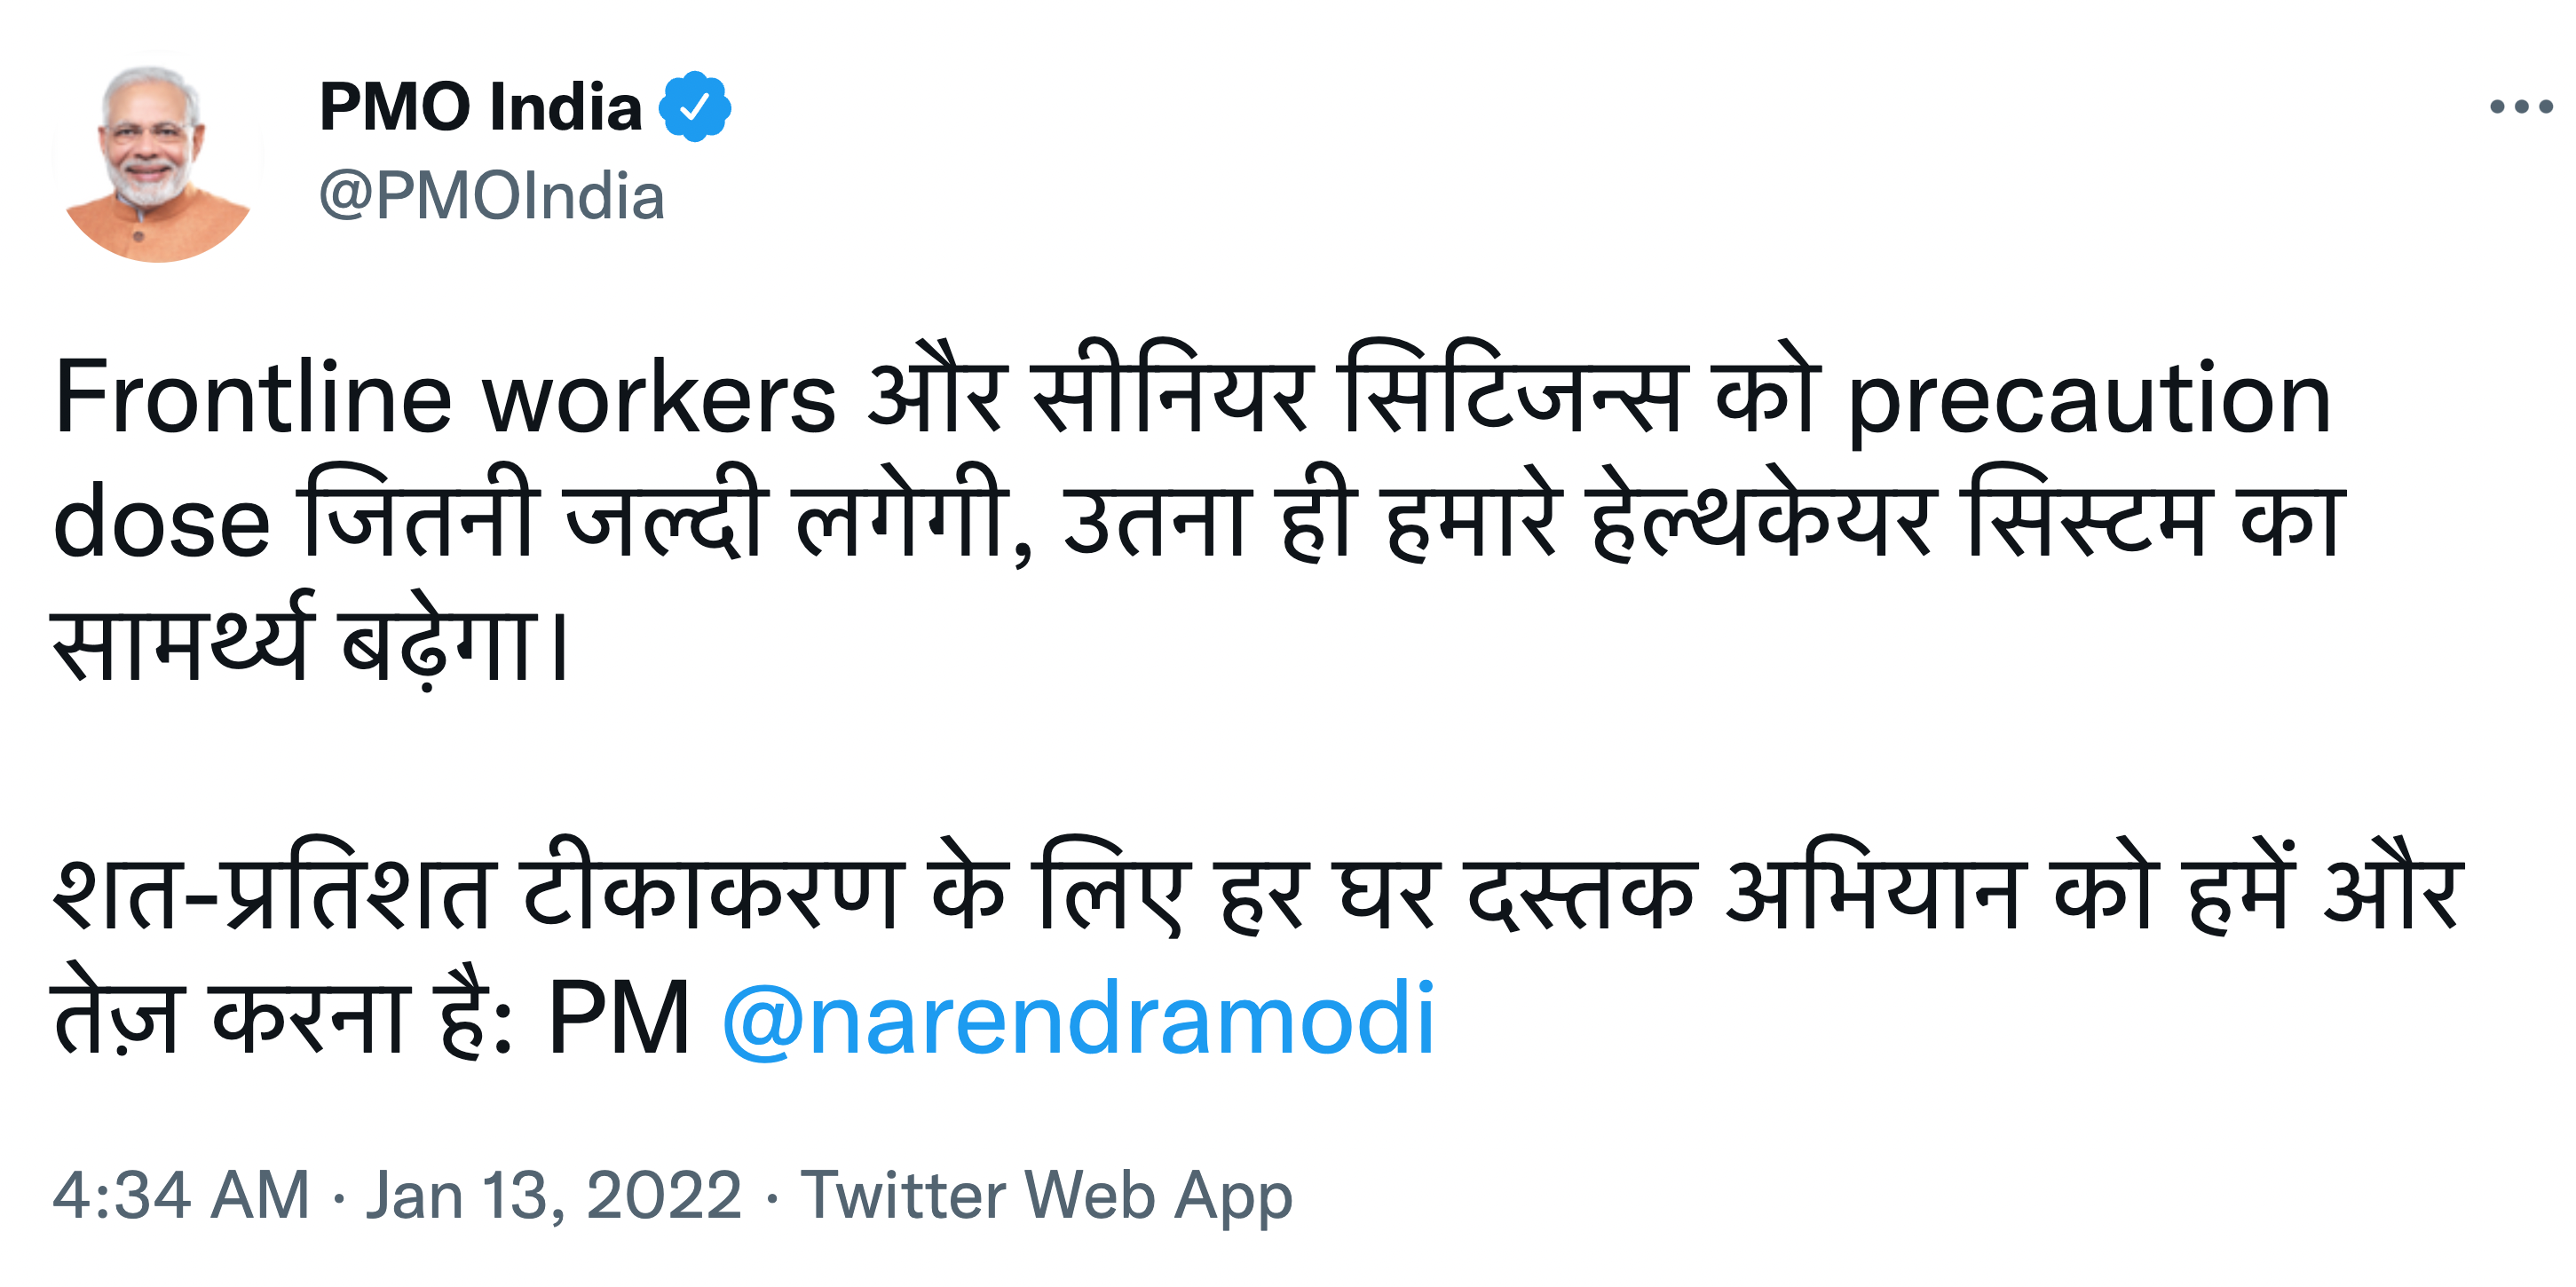
\includegraphics[width=\linewidth]{pmi-tweet-langswitch.png}
%    \caption{A tweet demonstrating language switching between English and Hindi; such seamless language switching is common in multilingual environments.}
%    \label{fig:example-langswitch}
%\end{figure}


\begin{figure}[ht]
    \centering
    \renewcommand{\arraystretch}{1.4}
    \begin{tabular}{ p{0.95\linewidth}}
    \hline
    Original: {``\textsf{bandaaginda bari} \textit{bageeche ke bahar}\textsf{-e iddivi.} \textit{kahaani ke andhar} \textsf{ bandu bidona.} \textit{kaam bolo saab.}"} \\ 
    \hdashline
    \textsf{Kannada: ``bandaaginda bari vishayada horagadene iddivi. katheya olagade bandu bidona. kelasa heli saar."}\\
    %\textcolor{OliveGreen}{Hindi: ``.''}\\
    English Translation:  ``From the time I've reached here, we've stayed outside of the topic. Let's come into the matter. Tell me the work, sir."\\
    \hline
    \end{tabular}
    \caption{Demonstration of language switching between \textsf{Kannada} and \textit{Hindi}.
    The original dialogue is taken from an Indian movie. Such seamless language switching is common among multilingual speakers.}
    \label{fig:example-langswitch-hinkan}
    
    
    \begin{comment}
    \vspace{5mm}
    \begin{tabular}{ p{0.95\linewidth}}
    \hline
    Original: \textit{``\textcolor{blue}{Ce moment} \textcolor{OliveGreen}{when you start} \textcolor{blue}{penser en deux langues} \textcolor{OliveGreen}{at the same} \textcolor{blue}{temps!}"} \\
    \textcolor{blue}{French: ``Ce moment quand vous commencez à penser en deux langues au même temps!"}\\
    \textcolor{OliveGreen}{English: ``The moment when you start to think in two languages at the same time!"}\\
    \hline
    \end{tabular}
    \caption{Demonstration of language switching between \textcolor{blue}{French} and \textcolor{OliveGreen}{English}.}
    \end{comment}
\end{figure}



In this chapter, we show that, multilingual NMT models, as commonly built, are \textit{not robust} to multi-sentence translation, especially when language switching is involved. The contributions of this chapter are outlined as follows:
Firstly, inspired by \textsc{CheckList}~\cite{ribeiro-etal-2020-beyond}, a few simple but effective checks for improving the test coverage in multilingual NMT evaluation are described (Section~\ref{sec:multiling-mt-checks}).
Secondly, we explore training data augmentation techniques such as concatenation and noise addition in the context of multilingual NMT (Section~\ref{sec:train-aug}).
Third, using a many-to-one multilingual translation task setup (Section~\ref{sec:setup}), we investigate the relationship between training data augmentation methods and their impact on multilingual test cases. 
Fourth, we conduct a glass-box analysis of cross-attention in the Transformer architecture and show visually as well as quantitatively that the models trained with concatenated training sentences learn a more sharply focused attention mechanism than others.
% \mg{Per Jon's comment, it can be replaced with ``more sharply focused''}(Section~\ref{sec:attn-bleed}).
Finally, we examine how our data augmentation strategies generalize to multi-sentence translation for a variable number of sentences, and determine that two-sentence concatenation in training is sufficient to model many-sentence concatenation in inference (Section~\ref{sec:generalization}). 

%\section{Language Alternation}
%\tg{TODO: write about language alternation. different kinds. why it is important. why it is challenging.}


%%%%%%%%%%%%%%%%%%%%%%%%%%SECTION%%%%%%%%%%%%%%%%%%%%%%%%%%%%%%%%%%%
\section{Multilingual Translation Evaluation: Additional Checks}
\label{sec:multiling-mt-checks}

Inspired by the behavior testing paradigm in software engineering, \citet{ribeiro-etal-2020-beyond} propose a \textsc{CheckList} to test beyond the accuracy of NLP models.
The central idea of \textsc{CheckList} is that given any held-out set, one can improve the coverage of testing by modifying the set in a systematic way designed to test linguistic capabilities of natural language processing (NLP) modeling.
Some of the modifications \textsc{CheckList} employs are: synonym replacement, named entity replacement, negation, etc. 
Although these modifications are straightforward in tasks such as sentiment classification, such modifications on parallel sentences while maintaining the consistency on both sides is not trivial.
%are non-trivial in machine translation between varieties of languages.
%For instance, 
Nevertheless, the principles of behavior testing and their application to improve test coverage in machine translation are intriguing. 
We, therefore, explore suitable checks in the context of multilingual NMT. 

\textit{Definitions:} Translation tasks are categorized as \textit{bilingual} if a single source language is translated to a single target language, and \textit{multilingual} if two or more languages are on either of the source or target side. Multilingual tasks are further sub-classified based on the number of languages and the side they on are as many-to-one, one-to-many, and many-to-many. 
In this chapter, we focus on many-to-one (i.e., many source languages, one target) multilingual translation.

\textit{Notation:} For simplicity, consider a many-to-one model that translates sentences from $K$ source languages,  $\{L_k | k = 1, 2, ... K\}$, to a target language, $T$.
Let $x_{i}^{(L_k)}$ be a sentence in the source language $L_k$, and let its translation in the target language be $y_{i}^{(T)}$; where unambiguous, we omit the superscripts.

We propose the following checks to be used for multilingual NMT:
%  refer to Table~\ref{tab:test-aug} for a summary
\begin{description}[itemsep=-2mm,topsep=0mm,leftmargin=3mm]
    
    \item[C-SL:] Concatenate consecutive sentences in the same language. 
    It is not always trivial to determine sentence segmentation in continuous language. This check thus tests if the model is invariant to a missed segmentation. 
    This check is possible iff held-out set sentence order preserves the coherency of the original document. 
    %\code{(x$_{i}$ ␣ x$_{i+1}$) $\rightarrow$ (y$_{i}$ ␣ y$_{i+1}$)}
    Formally, $$x^{(L_k)}_{i} + x^{(L_k)}_{i+1} \rightarrow y_i + y_{i+1}$$
    
    In practice, we use a space character to join sentences, indicated by the concatenation operator `$+$'.\footnote{We focus on orthographies that use space as a word-breaker.
    In orthographies without a word-breaker, joining may be performed without any glue character.}
    \item[C-TL:] Consecutive sentences in the source and target languages.
    This check tests if the MT system can preserve phrases that are already in the target language, and if the MT system can translate in the presence of code and language switching settings. For completeness, we can test both source-to-target and target-to-source language switching, as follows:
    \begin{align*}
       x^{(L_k)}_i + y_{i+1} & \rightarrow y_i + y_{i+1} \\
       y_{i} + x^{(L_k)}_{i+1} & \rightarrow y_{i} + y_{i+1}
    \end{align*}
Similar to C-SL, this check also requires the held-out set sentence order to preserve the coherency of the original document.
    %Similar to do-not-translate. Tests if model detects target language and preserves it. Assumption: test sentence preserves original document order.\\
    %\code{(x$_{i}$  ␣ y$_{i+1}$) $\rightarrow$ (y$_{i}$  ␣ y$_{i+1}$)} \\
    %\code{(y$_{i-1}$ ␣ x$_{i}$) $\rightarrow$ (y$_{i-1}$ ␣  y$_{i}$)}
    
    \item[C-XL:] This check tests if a multilingual MT system is agnostic to language switching. 
    This check is created by concatenating consecutive sentences across source languages. 
    This is possible iff the held-out sets are multi-parallel across languages, and, similar to the previous two, each preserves the coherency of the original documents.
    Given two languages $L_k$ and $L_m$, we obtain a test sentence as follows: 
    $$x^{(L_k)}_i + x^{(L_m)}_{i+1} \rightarrow y_i + y_{i+1}$$
    
    \item[R-XL:] This check tests if a multilingual MT system can function in light of a topic switch among its supported source languages. 
    % \mg{is competence the actual intended word here? what does competence languages mean?}
    For any two languages $L_k$ and $L_m$ and random positions $i$ and $j$ in their original corpus, we obtain a test segment by concatenating them as: 
    $$ x^{(L_k)}_i + x^{(L_m)}_j \rightarrow y_i + y_j $$
     This method makes the fewest assumptions about the nature of held-out datasets, i.e., unlike previous methods, neither multi-parallelism nor coherency in sentence order is necessary.
 \end{description}
 
 %For each of the above augmentations, its reference sentence is obtained by concatenating the corresponding parallel counterparts in the target language. 

%%%%========== COMMENT==========
\begin{comment}  
\begin{table}[htb]
\centering
\renewcommand{\arraystretch}{1.5}
\begin{tabular}{l l l }
\hline
    \textbf{Name} & \textbf{Source} & \textbf{Target} \\ 
\hline
    C-SL & $x^{(L_k)}_{i} + x^{(L_k)}_{i+1}$ & $y_i + y_{i+1}$ \\ \hdashline
\multirow{2}{*}{C-TL} & $x^{(L_k)}_i + y_{i+1}$ & $y_i + y_{i+1}$ \\
     & $y_{i-1} + x^{(L_k)}_{i}$ & y$_{i-1} + y_{i}$ \\ \hdashline
    C-XL & $x^{(L_k)}_i + x^{(L_m)}_{i+1}$ & $y_i + y_{i+1}$ \\
    R-XL & $x^{(L_k)}_i + x^{(L_m)}_j$ & $y_i + y_j$ \\
\hline
\end{tabular}
\caption{Held-out dataset augmentation methods. The operator `$+$' is concatenation with a space character.}
\label{tab:test-aug}
\end{table}
\end{comment}
%%%%========== COMMENT==========


%%%%%%%%%%%%%%%%%%%%%%%%%%SECTION%%%%%%%%%%%%%%%%%%%%%%%%%%%%%%%%%%%
\section{Improving Robustness via Data Augmentation Methods}
\label{sec:train-aug}
In the previous section, we described several ways of improving \textit{test} coverage for multilingual translation models.
In this section, we explore \textit{training} data augmentation techniques to improve robustness to language switching settings.

\subsection{Concatenation}
Concatenation of training sentences has been proven to be a useful data augmentation technique; \citet{nguyen-etal-2021-data} investigate key factors behind the usefulness of training segment concatenations in \textit{bilingual} settings. 
Their experiments reveal that concatenating random sentences performs as well as consecutive sentence concatenation, which suggests that discourse coherence is unlikely the driving factor behind the gains.
They attribute the gains to three factors: context diversity, length diversity, and position shifting.

In this chapter, we investigate training data concatenation under \textit{multilingual} settings, hypothesizing that concatenation helps achieve the robustness checks that are described in the prior section. Our training concatenation approaches are similar to our check sets, with the notable exception that we do not consider consecutive sentence training specifically, both because of \citet{nguyen-etal-2021-data}'s finding and because training data gathering techniques can often restrict the availability of consecutive data \cite{banon-etal-2020-paracrawl}.  
We investigate the following sub-settings for concatenations:

\begin{description}[itemsep=0.5mm,topsep=0pt,leftmargin=5mm]
\item[CatSL:] Concatenate a pair of source sentences in the same language, using space whenever appropriate (e.g. languages with space separated tokens). 
%\code{(x$_i$ ␣ x$_j$) $\rightarrow$ (y$_i$ ␣ y$_j$)} where \code{x$_i$} and \code{x$_i$} are in the same language.
$$x^{(L_k)}_i + x^{(L_k)}_j \rightarrow y_i + y_j$$

\item[CatXL:] Concatenate a pair of source sentences, without constraint on language.
%\code{(x$_i$ ␣ x$_j$) $\rightarrow$ (y$_i$ ␣ y$_j)$} where $x_i$ and $x_j$ are not necessarily in the same language.
$$x^{(L_k)}_i + x^{(L_m)}_j \rightarrow y_i + y_j$$
\item[CatRepeat:] The same sentence is repeated and then concatenated. 
Although this seems uninteresting, it serves a key role in ruling out gains possibly due to data repetition and modification of sentence lengths.
%\code{(x$_i$ ␣ x$_i$) $\rightarrow$ (y$_i$ ␣ y$_i$)}
 $$x^{(L_k)}_i + x^{(L_k)}_i \rightarrow y_i + y_i$$
\end{description}

%Refer to Table~\ref{tab:train-aug} for an overview of these methods.
\subsection{Adding Noise}
We hypothesize that introducing noise during training might help achieve robustness, and investigate two approaches that rely on noise addition:
\begin{description}[itemsep=0.5mm,topsep=0pt,leftmargin=5mm]
\item[DenoiseTgt:] Form the source side of a target segment by adding noise to it. 
% \texttt{noise(y) $\rightarrow$ y}
Formally, $$noise(y; r) \rightarrow y$$ where, hyperparameter $r$ controls the noise ratio.
Denoising is an important technique in unsupervised NMT \cite{Artetxe-2018-unmt-iclr,Lample-2018-unmt-iclr}.

\item[NoisySrc:] Add noise to the source side of a translation pair.
% \code{noise(x) $\rightarrow$ y}
Formally, $$noise(x; r) \rightarrow y$$ 
This resembles back-translation~\cite{sennrich-etal-2016-improving} where augmented data is formed by pairing noisy source sentences with clean target sentences.

%\item[RevSrc:] Reverse the words in source segment and use it as input while the target is unmodified. 
% \code{reverse(y) $\rightarrow$ y}
% \code{reverse(x) $\rightarrow$ y}
%\item[RevTgt:]  Reverse the words in target segment and use it as input while target side is unmodified segment.
\end{description}

%Refer to Table~\ref{tab:train-aug} for an overview of these methods.
%Both RevSrc and RevTgt reverses word order while preserving the character order within words.
The function $noise(...; r)$ is implemented as follows: %for a given $r \in (0, 100)$, 
(i) $r\%$ of random tokens are dropped, 
(ii) $r\%$ of random tokens are replaced with random types uniformly sampled from vocabulary, and 
(iii) $r\%$ of random tokens' positions are displaced within a sequence.
We use $r=10\%$ in the experiments discussed in this chapter.

\begin{comment} %=======COMMENT=====
\begin{table}[htb]
\centering
\renewcommand{\arraystretch}{1.3}
\begin{tabular}{l l l}
\hline
    \textbf{Name}   & \textbf{Source} & \textbf{Target} \\
\hline
    CatSL      & $x^{(L_k)}_i + x^{(L_k)}_j$ & $y_i + y_j$ \\
    CatXL      & $x^{(L_k)}_i + x^{(L_m)}_j$ & $y_i + y_j$ \\
    CatRepeat  & $x^{(L_k)}_i + x^{(L_k)}_i$ & $y_i + y_i$ \\ \hdashline
    NoisySrc   & $noise(x)$ & $y$ \\
    DenoiseTgt & $noise(y)$ & $y$ \\
    %RevSrc     & $rev\_words(x)$ & $y$ \\    
    %RevTgt     & $rev\_words(y)$ & $y$ \\
\hline
\end{tabular}
\caption{Training data augmentation methods; Operator `$+$' is concatenation with a space character. }
\label{tab:train-aug}
\end{table}
%%% \ end{comment}

%\begin{comment}  % ==== COMMENT
\end{comment} 
%=======COMMENT=====


\renewcommand{\arraystretch}{1.2}
\begin{table}[htb]
    \centering
\begin{tabular}{l @{\hspace{6pt}} c @{\hspace{6pt}} r }
\hline
\textbf{Language} & \textbf{In-domain} & \multicolumn{1}{c}{\textbf{All-data}} \\
\hline
Bengali (BN)  & 23.3k/0.4M/0.4M    & 1.3M/19.5M/21.3M \\
Gujarati (GU) & 41.6k/0.7M/0.8M    & 0.5M/07.2M/09.5M \\
Hindi (HI)    & 50.3k/1.1M/1.0M    & 3.1M/54.7M/51.8M \\
Kannada (KN)  & 28.9k/0.4M/0.6M    & 0.4M/04.6M/08.7M \\
{Malayalam}(ML) & 26.9k/0.3M/0.5M  & 1.1M/11.6M/19.0M \\
Marathi (MR)  & 29.0k/0.4M/0.5M    & 0.6M/09.2M/13.1M \\
Oriya (OR)    & 32.0k/0.5M/0.6M    & 0.3M/04.4M/05.1M \\
Punjabi (PA)  & 28.3k/0.6M/0.5M    & 0.5M/10.1M/10.9M \\
Tamil (TA)    & 32.6k/0.4M/0.6M    & 1.4M/16.0M/27.0M \\
Telugu (TE)   & 33.4k/0.5M/0.6M    & 0.5M/05.7M/09.1M \\
\hdashline
All   & 326k/5.3M/6.1M     & 9.6M/143M/175M\\ 
\hline
\end{tabular} 
    \caption{Training dataset statistics: \textit{segments / source / target tokens}, before tokenization.}
    \label{tab:training-stats}
%\end{table}
\vspace{5mm}
%\begin{table}[htb]
    \centering
\begin{tabular}{l c c}
\hline
\textbf{Name} & \textbf{Dev} & \textbf{Test} \\
\hline
Orig & 10k/140.5k/163.2k & 23.9k/331.1k/385.1k \\
C-SL & 10k/281.0k/326.4k & 23.9k/662.1k/770.1k \\
C-TL & 10k/303.7k/326.4k & 23.9k/716.1k/770.1k \\
C-XL & 10k/283.9k/326.4k & 23.9k/670.7k/770.1k \\
R-XL & 10k/216.0k/251.2k & 23.9k/514.5k/600.5k \\
\hline
\end{tabular}
    \caption{Development and test set statistics: \textit{segments / source / target tokens}, before tokenization. 
    The row named `Orig' is the union of all ten individual languages' datasets, and the rest are created as per definitions in Section~\ref{sec:multiling-mt-checks}.
    Dev-Orig set is used for validation and early stopping in all our multilingual models.}
    \label{tab:heldout-stats}
\end{table}


\begin{table}[htb]
    \centering
    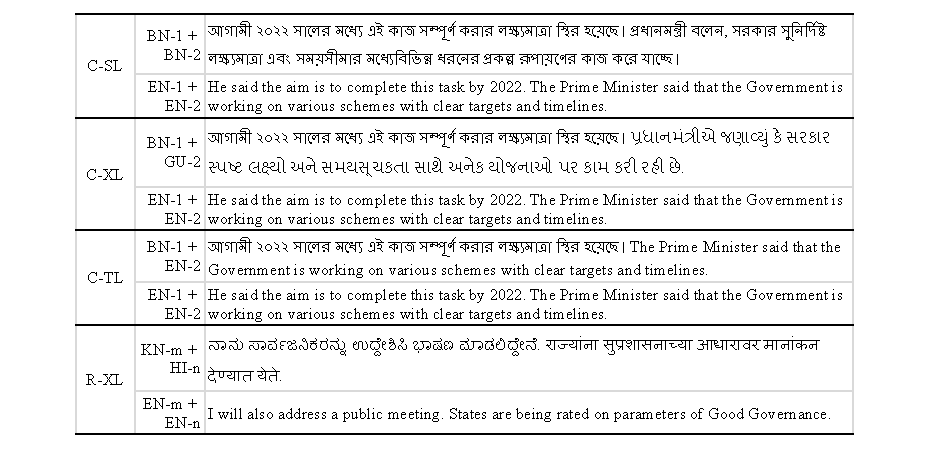
\includegraphics[width=0.99\linewidth,trim={12mm 2mm 12mm 2mm},clip]{img/robustness/example-concat-devs.pdf}
    \caption{Concatenated sentence examples from the development set. 
    Bengali (BN), Gujarati (GU), Kannada (KN), and Hindi (HI) are chosen for illustrations; similar augmentations are performed for all other languages in the corpus.
    Indices $1$ and $2$ indicate consecutive positions, and $m$ and $n$ indicate random positions.}
    \label{tab:dev-aug-example}
\end{table}

%%%%%%%%%%%%%%%%%%%%%%%%%%SECTION%%%%%%%%%%%%%%%%%%%%%%%%%%%%%%%%%%%
\section{Setup}
\label{sec:setup}

\subsection{Dataset}
\label{ch:rtobustness-sec:dataset}
We use publicly available datasets from The Workshop on Asian Translation 2021 (WAT21)'s  \textit{MultiIndicMT}~\cite{nakazawa-etal-2021-overview}\footnote{\url{http://lotus.kuee.kyoto-u.ac.jp/WAT/indic-multilingual/}} shared task. This task involves translation between English(EN) and 10 Indic Languages, namely: Bengali(BN), Gujarati(GU), Hindi(HI), Kannada(KN), Malayalam(ML), Marathi(MR), Oriya(OR), Punjabi(PA), Tamil(TA) and Telugu(TE). 
The development and held-out test sets are multi-parallel and contain 1,000 and 2,390 sentences, respectively. 
The training set contains a small portion of data from the same domain as the held-out sets, as well as additional datasets from other domains.
All the training data statistics are given in Table~\ref{tab:training-stats}.
We focus on the Indic$\shortarrow$English (many-to-one) translation direction in this chapter.

Following the definitions in Section~\ref{sec:multiling-mt-checks}, we create C-SL, C-TL, C-XL, and R-XL versions of development and test sets; statistics are given in Table~\ref{tab:heldout-stats}. 
An example demonstrating the nuances in all these four methods is shown in Table~\ref{tab:dev-aug-example}. 
Following the definitions in Section~\ref{sec:train-aug}, we create CatSL, CatXL, CatRpeat, DenoiseTgt, and NoisySrc augmented training segments. 
For each of these training corpus augmentation methods, we restrict the total augmented sentences to be roughly the same number of segments as the original corpus, i.e., 326k and 9.6M segments in the in-domain and the all-data setup, respectively.


\subsection{Model and Training Process}

We use a Transformer base model \cite{vaswani-2017-attention}, similar to the one used in Chapter~\ref{ch:nlg-imbalance}, having 512 hidden dimensions, 6 encoder and decoder layers, 8 attention heads, and intermediate feedforward layers of 2048 dimensions.
We use our PyTorch based NMT toolkit (Section~\ref{sec:rtg}).
% named RTG \cite{gowda-etal-2021-many} to train all our models.\footnote{\url{https://isi-nlp.github.io/rtg/}}.
As described in Chapter~\ref{ch:nlg-imbalance}, tuning the vocabulary size and batch size are important to achieve competitive performance.
We use byte-pair-encoding (BPE) \cite{sennrich-etal-2016-bpe}, with vocabulary size adjusted as per our findings in Chapter~\ref{ch:nlg-imbalance}. %, except, to avoid extremely large vocabularies which are infeasible in practice, we place a maximum limit of 500k and 128k types on source and target, respectively\footnote{Largest vocabulary sizes found are 230k and 63k}.
Since the source side has many languages and the target side has only a single language, we use a larger source vocabulary than that of the target.
The source side vocabulary contains BPE types from all 11 languages (i.e., ten source languages and English), whereas to improve the efficiency in the decoder's softmax layer, the target vocabulary is restricted to contain English only. 
Our in-domain limited-data setup learns BPE vocabularies of 30.4k and 4.8k types for source and target languages.
Similarly, the all-data setup learns 230.4k and 63.4k types.
The training batch size used for all our multilingual models is 10k tokens for the in-domain limited-data setup, and 25k tokens for the larger all-data setup.
The batch size for the baseline bilingual models is adjusted as per data sizes using \textit{`a thousand per million tokens'} rule of thumb that we have come to devise with a maximum of 25k tokens.
% \mg{citation for this?}\tg{no citation available; this is something I found while redoing NMT Learning curve (V2) that never got published}.
 The median sequence lengths in training after subword segmentation but before sentence concatenation are 15 on the Indic side and 17 on the English side. 
 We model sequence lengths up to 512 time steps during training.
%i.e., for a dataset having \code{w} target language tokens, the adjusted batch size is as per (Python) function: \code{min(25000, round(w/1000, -3))}.
We use the same learning rate schedule as \citet{vaswani-2017-attention}.
We train our models until a maximum of 200k optimizer steps, and use early stopping with patience of 10 validations.
Validations are performed after every 1000 optimizer steps.
All our models are trained using one Nvidia A40 GPU per setting. 
The smaller in-domain setup takes less than 24 hours per run, whereas the larger all-data setup takes at most 48 hours per run (or less when early stopping criteria are reached).
We run each experiment two times and report the average. During inference, we average the last 5 checkpoints and use a beam decoder of size 4 and length penalty of $\alpha=0.6~$\cite{vaswani-2017-attention,wu-etal-2016-GNMT}. 


\begin{table*}[h!t]
\centering
%\small
\setlength{\tabcolsep}{4pt}
\begin{tabular}{l | rr | rrrrr rrrrr}
\hline
& Dev & Test & BN & GU & HI & KN & ML & MR & OR & PA & TA & TE \\
\hline
{WAT21 biling indomain~\ddag} & & 18.6 & 11.3 & 26.2 & 28.2 & 20.3 & 13.6 & 15.1 & 16.4 & 23.7 & 16.1 & 14.7 \\
{Biling; indomain~\ddag} & 24.1 & 21.6 & 13.2 & 29.3 & 32.9 & 22.7 & 17.9 & 16.9 & 16.4 & 27.4 & 18.1 & 21.0 \\ \hdashline 
{Biling; indomain} & 23.9 & 21.5 & 13.1 & 29.2 & 32.6 & 22.5 & 17.7 & 16.8 & 16.4 & 27.3 & 18.0 & 20.9 \\
{Many-to-one; indomain} & 26.5 & 22.7 & 18.7 & 25.7 & 27.8 & 23.1 & 21.2 & 20.8 & 21.1 & 25.8 & 20.6 & 22.4 \\
{Many-to-one; all data} & 35.0 & 32.4 & 26.2 & 36.8 & 40.1 & 31.7 & 30.0 & 29.8 & 30.5 & 38.8 & 29.1 & 30.8 \\ 
\hline
\end{tabular} 
\caption{Indic$\shortarrow$English BLEU scores.
Rows indicated by \ddag{} match the evaluation settings used by WAT21 shared task (i.e., tokenized BLEU). 
The rows without \ddag{} are detokenized BLEU obtained from \textsc{SacreBLEU} \cite{post-2018-sacrebleu}. 
Dev and Test are average across 10 languages.
}
\label{tab:bleu-base}
\end{table*}

%\vspace{2mm}
%\renewcommand{\arraystretch}{1.2}
\begin{table*}[htb]
\centering
%\small
\setlength{\tabcolsep}{4pt}
\begin{tabular}{l l rrrrr : rrrrr}
\hline
& & \multicolumn{5}{c:}{\textbf{Dev}} & \multicolumn{5}{c}{\textbf{Test}} \\
ID & In-domain & Avg & C-TL & C-SL & C-XL & R-XL & Avg & C-TL & C-SL & C-XL & R-XL \\
\hline
\#I1 & Baseline (B)            & 26.5 & 10.8 & 17.0 & 16.9 & 15.9               & 22.7 & 9.4 & 14.9 & 14.7 & 13.6 \\
\hdashline
\#I2 & B+CatRepeat & 25.3 & 9.9 & 14.5 & 14.7 & 13.3 & 21.6               & 8.6 & 13 & 13 & 11.4 \\ 
\#I3 & B+CatXL     & 26.2 & 12.6 & 26.1 & 25.9 & \textbf{26.5} & 22.6 & 11.1 & 22.7 & 22.5 & 22.3 \\
\#I4 & B+CatSL     & 26.1 & 13.2 & 26.1 & 25.9 & \textbf{26.5} & 22.6 & 11.4 & 22.9 & \textbf{22.6} & 22.3 \\
\#I5 & B+NoisySrc  & 25.2 & 10.5 & 16.2 & 16.0 & 15.2               & 21.2 & 9.1 & 14.3 & 14.1 & 12.9 \\
\#I6 & B+DenoiseTgt & \textbf{26.7} & 40.4 & 17.9 & 17.7 & 16.6    & \textbf{23.2} & {39.7} & 15.7 & 15.4 & 14.1 \\
%G & b+DenoiseTgtExt  & 26.5 & \hl{43.9} & 17.9 & 17.8 & 16.4          & 23.0 & \hl{42.8} & 15.8 & 15.5 & 14.2 \\
%H & b+RevSrc           & 24.6 & 8.7 & 15.1 & 15.0 & 14.1                & 21.0 & 7.4 & 13.3 & 13.1 & 12.0 \\
%I & b+RevTgt           & \hl{27.0} & 19.6 & 18.0 & 17.8 & 16.8          & \hl{23.4} & 18.4 & 15.9 & 15.6 & 14.3 \\
\hdashline
\#I7 & B+CatXL+DenoiseTgt & 26.1 & \textbf{55.2} & \textbf{26.3} & \textbf{26.0} & 26.4 & 22.6 & \textbf{53.4} & \textbf{23.0} & \textbf{22.6} & \textbf{22.4} \\ 
\hline
\end{tabular} 
\caption{ Indic$\shortarrow$English BLEU scores for models trained on in-domain training data only. The best scores are shown in bold. }
\label{tab:bleu-indom-aug}
%\end{table*}
\vspace{2mm}
%\begin{table*}[htb]
%    \centering
%    \small
\begin{tabular}{l l rrrrr : rrrrr}
\hline
& & \multicolumn{5}{c:}{\textbf{Dev}} & \multicolumn{5}{c}{\textbf{Test}} \\
ID & All-data & Avg & C-TL & C-SL & C-XL & R-XL & Avg & C-TL & C-SL & C-XL & R-XL \\
\hline
\#A1 & Baseline (B) & \textbf{35.0} & 43.1 & 30.0 & 29.5 & 28.2 & \textbf{32.4} & 42.2 & 27.8 & 27.3 & 26.1 \\
\hdashline
\#A2 & B+CatRepeat & 34.5 & 43.7 & 30.3 & 29.9 & 28.8 & 32.0 & 42.9 & 28.0 & 27.6 & 26.3 \\ 
\#A3 & B+CatXL  & 34.1 & 53.3 & 31.9 & \textbf{33.7} & \textbf{34.4} & 31.6 & 52.4 & 29.7 & \textbf{31.0} & \textbf{31.2} \\
\#A4 & B+CatSL & 33.6 & 54.0 & \textbf{32.5} & 32.2 & 34.3 & 31.3 & 53.3 & \textbf{30.4} & 29.9 & 31.1 \\
\#A5 & B+NoisySrc & 34.9   & 42.1 & 29.8 & 29.2 & 27.8 & 32.3 & 41.7 & 27.6 & 27.1 & 25.8 \\
\#A6 & B+DenoiseTgt      & 33.3 & 60.0 & 28.9 & 28.4 & 27.3 & 31.3 & 59.4 & 27.1 & 26.5 & 25.4 \\
%G & b+DenoiseTgtExt   & 32.9 & \hl{55.7} & 28.3      & 27.9 & 26.7 & 30.9 & \hl{55.4} & 26.6 & 26.0 & 24.8 \\
% H & b+RevSrc            & 34.4 & 43.2      & 29.1      & 28.7 & 27.4 & 32.0 & 42.5 & 27.2 & 26.6 & 25.5 \\
%I & b+RevTgt           & 33.8  & 51.8      & 29.7      & 29.0 & 27.9 & 31.4 & 51.3 & 27.6 & 27.0 & 26.0 \\
\hdashline
\#A7 & B+CatXL+DenoiseTgt & 33.3 & \textbf{65.8} & 31.1 & 33.0 & 33.6 & 31.0 & \textbf{64.7} & 28.9 & 30.4 & 30.3 \\ 
\hline
\end{tabular} 
\caption{Indic$\shortarrow$English BLEU scores for models trained on all data. \textit{Abbreviations:} Avg: average across ten languages, C-: consecutive sentences, R-: random sentences, TL: target-language (i.e, English), SL: same-language, XL: cross-language. The best scores are shown in bold font.}
\label{tab:bleu-alldata-augs}
\end{table*}

%\vspace{2mm}
\begin{table*}[htb]
\centering
\begin{tabular}{l l : rrrr : rrrr}
\hline
          &  & \multicolumn{4}{c:}{\textbf{Dev}} & \multicolumn{4}{c}{\textbf{Test}} \\
          ID &   & C-TL & C-SL & C-XL & R-XL & C-TL & C-SL & C-XL & R-XL \\ \hline
\#A1 & Baseline (B) & 14.3 & 10.4 & 10.3 & 10.1 & 14.3 & 10.6 & 10.5 & 10.3 \\
\#A2 & B+CatRepeat & 12.3 & 8.9 & 8.9 & 8.6 & 12.5 & 9.0 & 9.0 & 8.7 \\
 \#A3 & B+CatXL     &  {5.8} & 7.2 & 4.3 & 4.3 & 5.8 & {7.2} & 4.4 & 4.3 \\
 \#A4 & B+CatSL     & 5.3 & \textbf{6.2} & 6.1 & 5.2 & 5.4 & \textbf{6.2} & 6.2 & 5.2 \\
\#A5  & B+NoisySrc  & 17.4 & 16.1 & 16.1 & 15.8 & 17.5 & 16.2 & 16.2 & 15.9 \\
\#A6 & B+DenoiseTgt & 7.9 & 8.3 & 8.4 & 8.0 & 8.1 & 8.5 & 8.5 & 8.1 \\
%b+RevSrc & 13.6 & 11 & 10.9 & 10.7 & 13.7 & 11.1 & 11.1 & 10.8 \\
%b+RevTgt & 8.9 & 8.3 & 8.3 & 7.9 & 9.1 & 8.4 & 8.5 & 8.1 \\
%b+DenoiseTgtExt & 9.5 & 9.7 & 9.7 & 9.4 & 9.6 & 9.9 & 9.9 & 9.5 \\ 
\hdashline
 \#A7 & B+CatXL+DenoiseTgt & \textbf{4.3} & 6.8 & \textbf{3.9} & \textbf{4.1} & \textbf{4.4} & 7.0 & \textbf{4.0} & \textbf{4.1} \\ 
\hline
\end{tabular} 
\caption{Cross-attention bleed rate (lower is better); all numbers have been scaled from $[0,1]$ to $[0, 100]$ range for easier interpretation.
Models trained on concatenated sentences have lower attention bleed rate. Denoising is better than baseline, but not as much as concatenation. 
The lowest bleed rate is achieved by using both concatenation and denoising methods. The best scores are shown in bold font.}
\label{tab:xattn-bleed}
\end{table*}



%%%%%%%%%%%%%%%%%%%%%%%%%%SECTION%%%%%%%%%%%%%%%%%%%%%%%%%%%%%%%%%%%
\section{Results and Analysis}
\label{sec:results-and-analysis}

First, to test our setup with its various hyperparameters such as vocabulary and batch size, we train bilingual models using in-domain data, similar to WAT21 organizer baselines.
As shown in Table~\ref{tab:bleu-base}, our baselines achieve competitive BLEU scores~\cite{papineni-etal-2002-bleu}.\footnote{WAT21 baseline scores are obtained from \url{http://lotus.kuee.kyoto-u.ac.jp/WAT/evaluation/}, which reports BLEU using an external tokenizer script (\code{moses-tokenizer.perl}). 
Apart from the row tagged $\ddag$ in Table~\ref{tab:bleu-base}, which is intended to provide direct comparison to baselines, all other BLEU scores are
obtained using \textsc{SacreBLEU} with signature: \texttt{BLEU+case.mixed+numrefs.1+smooth.exp+tok.13a+version.1.4.13.}} 
Next, we train multilingual many-to-one models for both in-domain and all data.

Table~\ref{tab:bleu-indom-aug} presents our results from a limited quantity in-domain dataset.
The baseline model (\#I1) has strong performance on individual sentences, but degrades on held-out sets involving missed sentence segmentation and language switching.
Experiments with concatenated data, namely CatXL (\#I3) and CatSL (\#I4), while they appear to make no improvements on regular held-out sets, make a significant improvement in BLEU scores on C-SL, C-XL, and R-XL.
Furthermore, both CatSL and CatXL show a similar trend.
While they also make a small gain on the C-TL setting, DenoiseTgt method is clearly an out-performer on C-TL.
The model that includes both concatenation and denoising (\#I7) achieves consistent gains across all the robustness check columns.
In contrast, the CatRepeat (\#I2) and NoisySrc (\#I5) methods do not show any gains.

Our results from the all-data setup are provided in Table~\ref{tab:bleu-alldata-augs}. 
While none of the augmentation methods appear to surpass baseline BLEU on the regular held-out sets (i.e., Avg column), their improvements to robustness can be witnessed similar to the in-domain setup. 
We show a qualitative example in Table~\ref{tab:fig:example-translations}.


\begin{table}[htb]
    \centering
    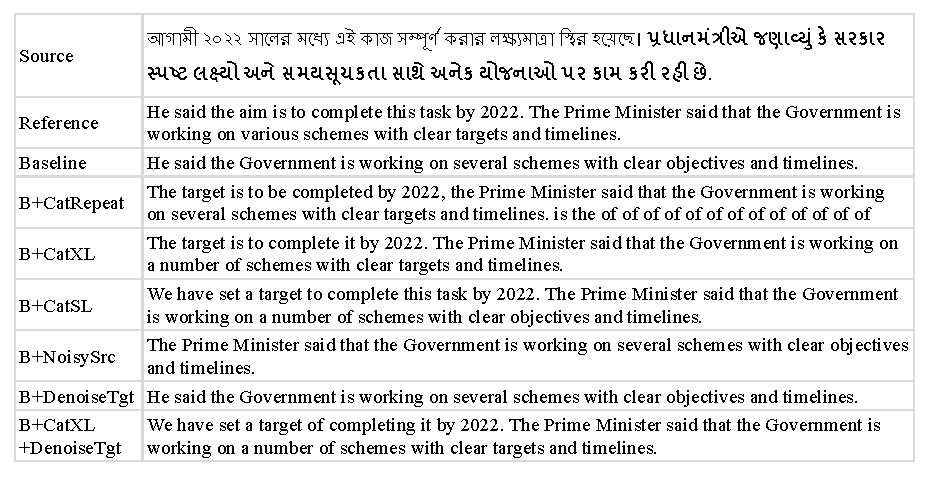
\includegraphics[width=0.98\linewidth,trim={2mm 2mm 2mm 2mm},clip]{img/robustness/example-translations.pdf}
    \caption{Example translations from the models trained on all-data setup.
    See Table~\ref{tab:bleu-alldata-augs} for quantitative scores of these models, and Figure \ref{fig:attnviz-catXL}  for a visualization of cross-attention.}
    \label{tab:fig:example-translations}
\end{table}
% and \ref{fig:attnviz-catXL+denoise}

\subsection{Attention Bleed}
\label{sec:attn-bleed}
% and \ref{fig:attnviz-catXL+denoise} 
Figure~\ref{fig:attnviz-catXL} visualizes cross-attention\footnote{Also known as encoder-decoder attention.} from our baseline model without augmentation as well as models trained with augmentation. 
Generally, the NMT decoder is run autoregressively; however, to facilitate the analysis described in this section, we force-decode reference translations and extract cross-attention tensors from all models.
%Since the sentence boundaries are required to determine the alignment of concatenated sentences,  we force-decode the reference translation that has known sentence boundaries.
The cross-attention visualization between a pair of concatenated sentences, say $(x_{i1} + x_{i2} \rightarrow y_{i1} + y_{i2})$, shows that models trained on augmented datasets appear to have less cross-attention mass across sentences, i.e., in the attention grid regions representing $x_{i2} \leftarrow y_{i1}$, and $x_{i1} \leftarrow y_{i2}$. 
We call attention mass in such regions \textit{attention bleed}. 
This observation confirms some of the findings suggested by \citet{nguyen-etal-2021-data}. 
We quantify attention bleed as follows: 
consider a Transformer NMT model with $L$ layers, each having $H$ attention heads and a held-out dataset of $\{(x_i ~ y_i) | i=1,2,...N\}$ segments. 
Furthermore, let each segment $(x_i, y_i) $ be a concatenation of two sentences, i.e. $(x_{i1}+ x_{i2}, ~ y_{i1}+y_{i2})$, with known sentence boundaries.
Let $|x_i|$ and $|y_i|$ be the sequence lengths after BPE segmentation, and $|x_{i1}|$ and $|y_{i1}|$ be the indices of the end of the first sentence (i.e., the sentence boundary) on the source and target sides, respectively.
%Therefore, the cross-attention tensor $A$ has the size $[ N x  L \times H \times |y_i| \times |x_i|]$.
% oops 5 dimensions will blew my mind. 
The average attention bleed across all the segments, layers, and heads is defined as:
$$ \bar{B} = \frac{1}{N \times L \times H} \sum_{i=1}^N \sum_{l=1}^L \sum_{h=1}^H b_{i,l,h}$$

\noindent where $b_{i,l,h}$ is the attention bleed rate in an attention head $h\in[1, H]$, in layer $l \in [1, L]$, for a single record at $i\in[1,N]$. 
To compute $b_{i,l,h}$, consider that an attention grid $A^{(i,l,h)}$ is of size $|y_i|\times|x_i|$. Then 
%Consider the attention bleed rate in an attention head $h\in[1, H]$ from layer $l \in [1, L]$, for a single record at $i\in[1,N]$. 
%The cross-attention grid $A$ is has the size of $|y_i|\times|x_i|$. 
%The attention bleed for segment $i$ in head $h$ at layer $l$ is given by $$
$$ b_{i,l,h} = \frac{1}{|y_i|} \Big[
      \sum_{t=1}^{|y_{i1}|} \sum_{s=|x_{i1}|+1}^{|x_i|} A^{(i,l,h)}_{t,s} 
    + \sum_{t=|y_{i1}|+1}^{|y_i|} \sum_{s=1}^{|x_{i1}|} A^{(i,l,h)}_{t,s} \Big] $$

%The average attention bleed across all the segments, layers, and heads as follows:
%$$ B = \frac{1}{N \times L \times H} \sum_{i=1}^N \sum_{l=1}^L \sum_{h=1}^H b_{i,l,h}$$

%%%%%%%%% COMMENT %%%%
\begin{comment}
Attention bleed rate for a single record $i$ having two concatenated sentences is given by:
\begin{multline*}
 B_i = \frac{1}{L \times H \times |y_i|} \sum_{l=1}^{L} \sum_{h=1}^{H} \bigg[ \sum A_{l,h}[y_{i1}, x_{i2}]\\ + \sum A_{l,h}[y_{i2}, x_{i1}] \bigg]
\end{multline*}
\noindent where $|y_i|$ is the number of tokens in the target sentence $y_{i1} + y_{i2}$ after BPE segmentation, $A[y_{i1}, x_{i2}]$ is the sum of attention paid by tokens in target sentence $y_{i1}$ to $x_{i2}$, and $A[y_{i2}:x_{i1}]$ is the sum of attention paid by target sentence $y_i2$ to $x_{i1}$. 
We compute average attention bleed across a corpus of $N$ such segments, as $$\bar{B} = \frac{1}{N} \sum_{i=1}^N B_i$$
\end{comment}
%%%%%%%%% COMMENT %%%%
\noindent where $A^{(i,l,h)}_{t,s}$ is the percent of attention paid to source position $s$ by target position $t$ at decoder layer $l$ and head $h$ in record $i$. Intuitively, a lower value of $\bar{B}$ is better, as it indicates that the model has learned to pay attention to appropriate regions. 
 As shown in Table~\ref{tab:xattn-bleed}, the models trained on augmented sentences achieve lower attention bleed. 

\begin{figure}[h!tb]
    %\includegraphics[width=2mm,angle=90,trim={24cm 1mm 0mm 35mm},clip]{attnviz-SL-baseline-xttn.png}
    \centering
    \begin{subfigure}[b]{0.49\linewidth}
        \centering
        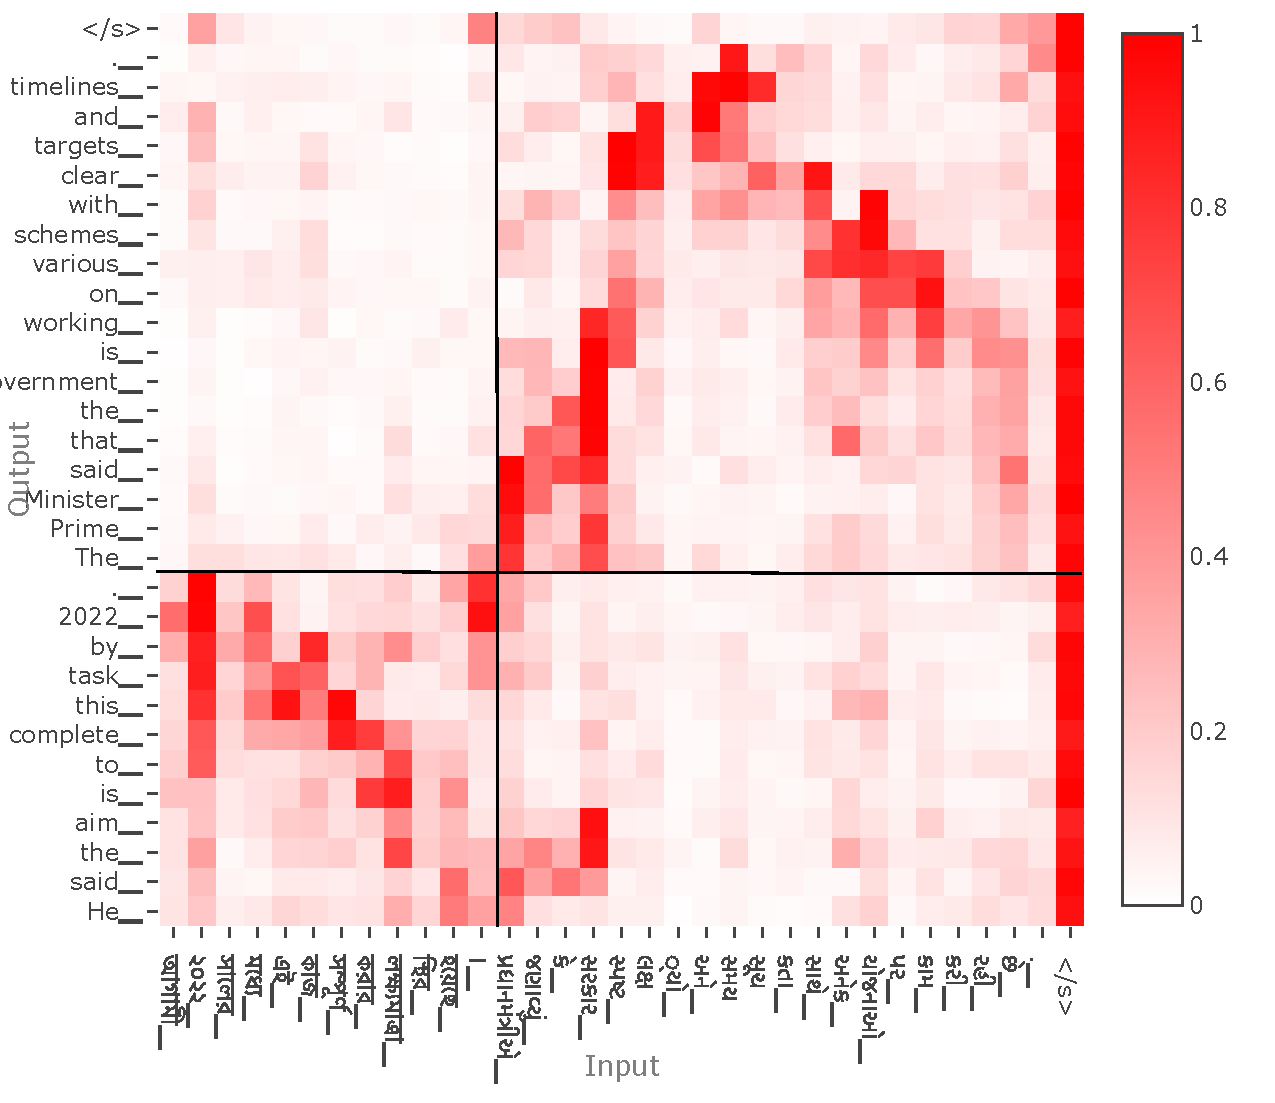
\includegraphics[width=\linewidth,trim={0mm 3mm 38mm 3mm},clip]{img/robustness/xattn-catXL-baseline-ann.pdf}
        \caption{Baseline without sentence concatenation (\#A1)}
        \label{fig:baseline-on-catXL}
     \end{subfigure}
    \begin{subfigure}[b]{0.49\linewidth}
        \centering
        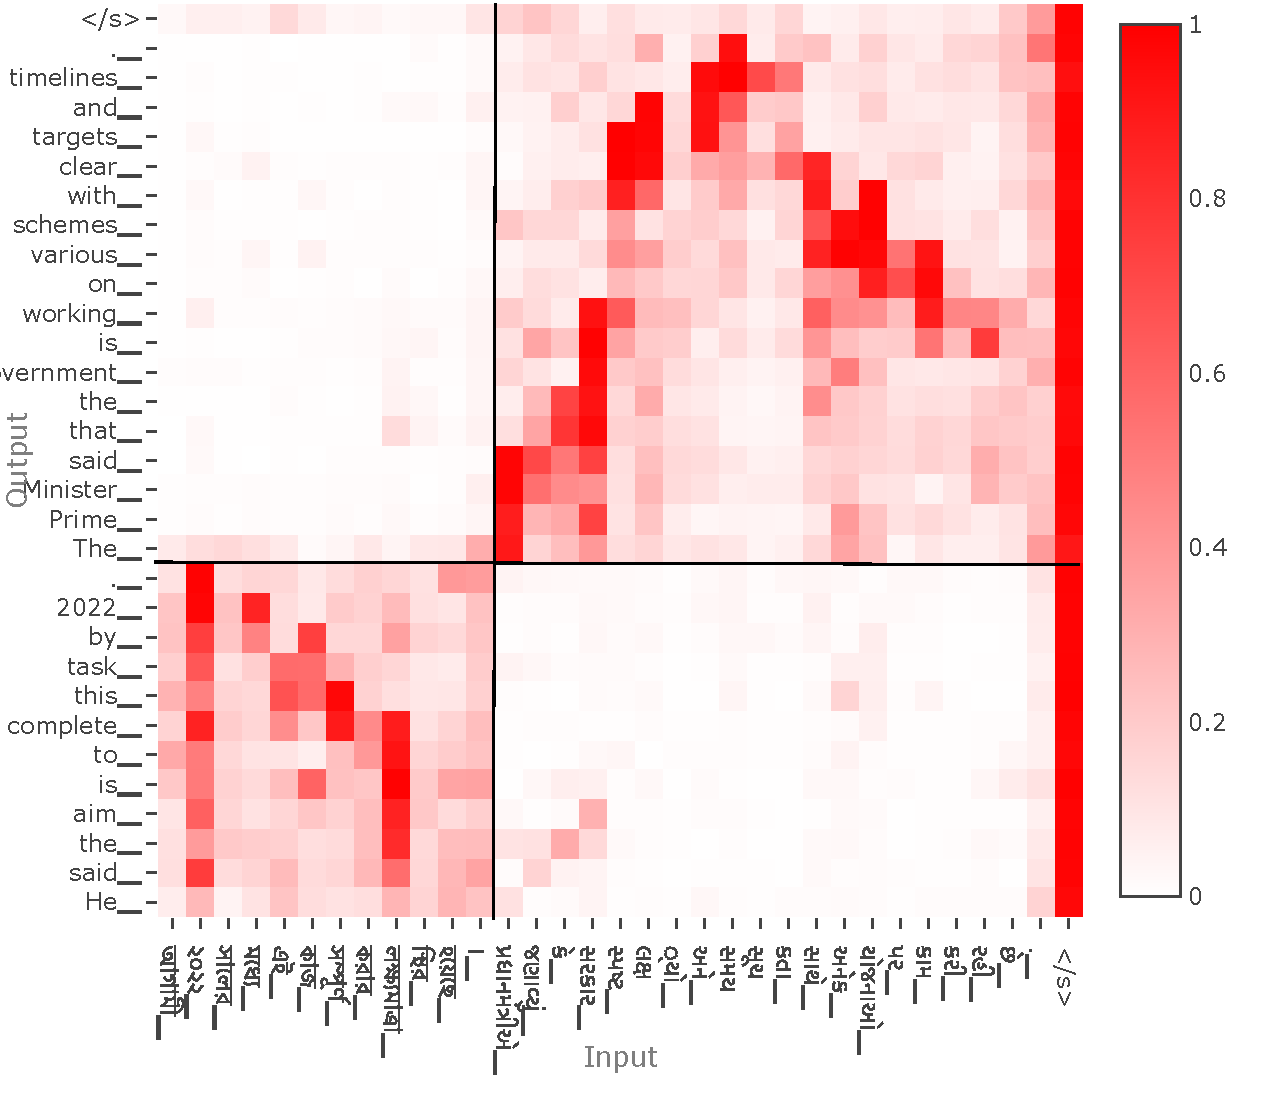
\includegraphics[width=\linewidth,trim={0mm 3mm 38mm 1mm},clip]{img/robustness/xattn-catXL-catXL-ann.pdf}
        \caption{Model trained with concatenated sentences (\#A3)}
        \label{fig:CatXL-on-CatXL}
     \end{subfigure}
   
   \vspace{5mm}
   
   \begin{subfigure}[b]{0.49\linewidth}
         \centering
         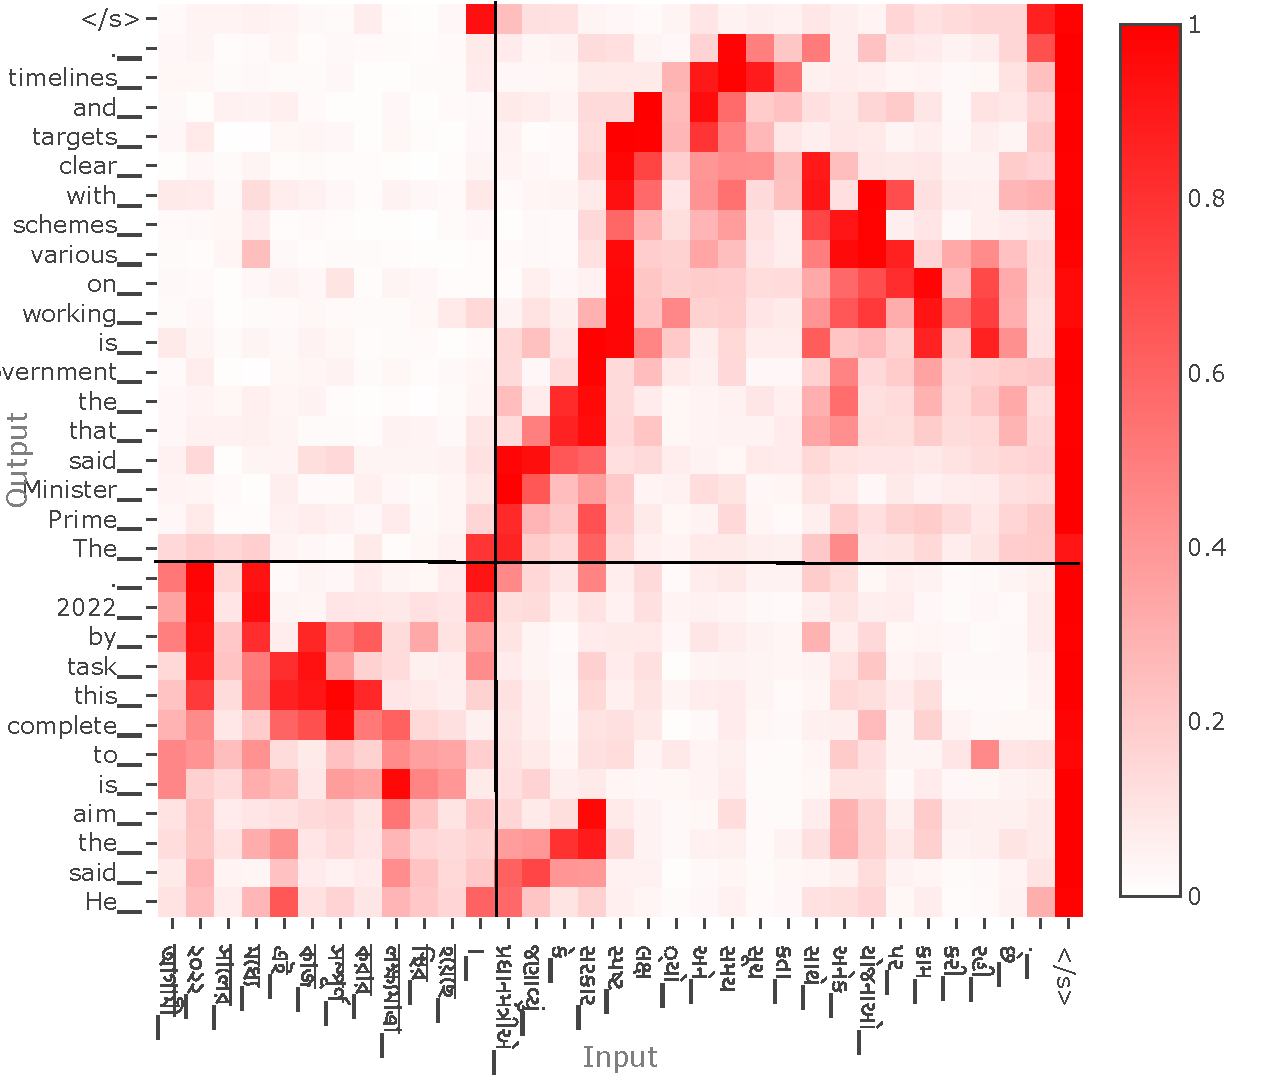
\includegraphics[width=\linewidth,trim={0mm 3mm 38mm 2mm},clip]{img/robustness/xattn-catXL-denoise-ann.pdf}
         \caption{Model trained with DenoiseTgt augmentation (\#A6)}
         \label{fig:denoise-on-catXL}
      \end{subfigure}
     \begin{subfigure}[b]{0.49\linewidth}
         \centering
         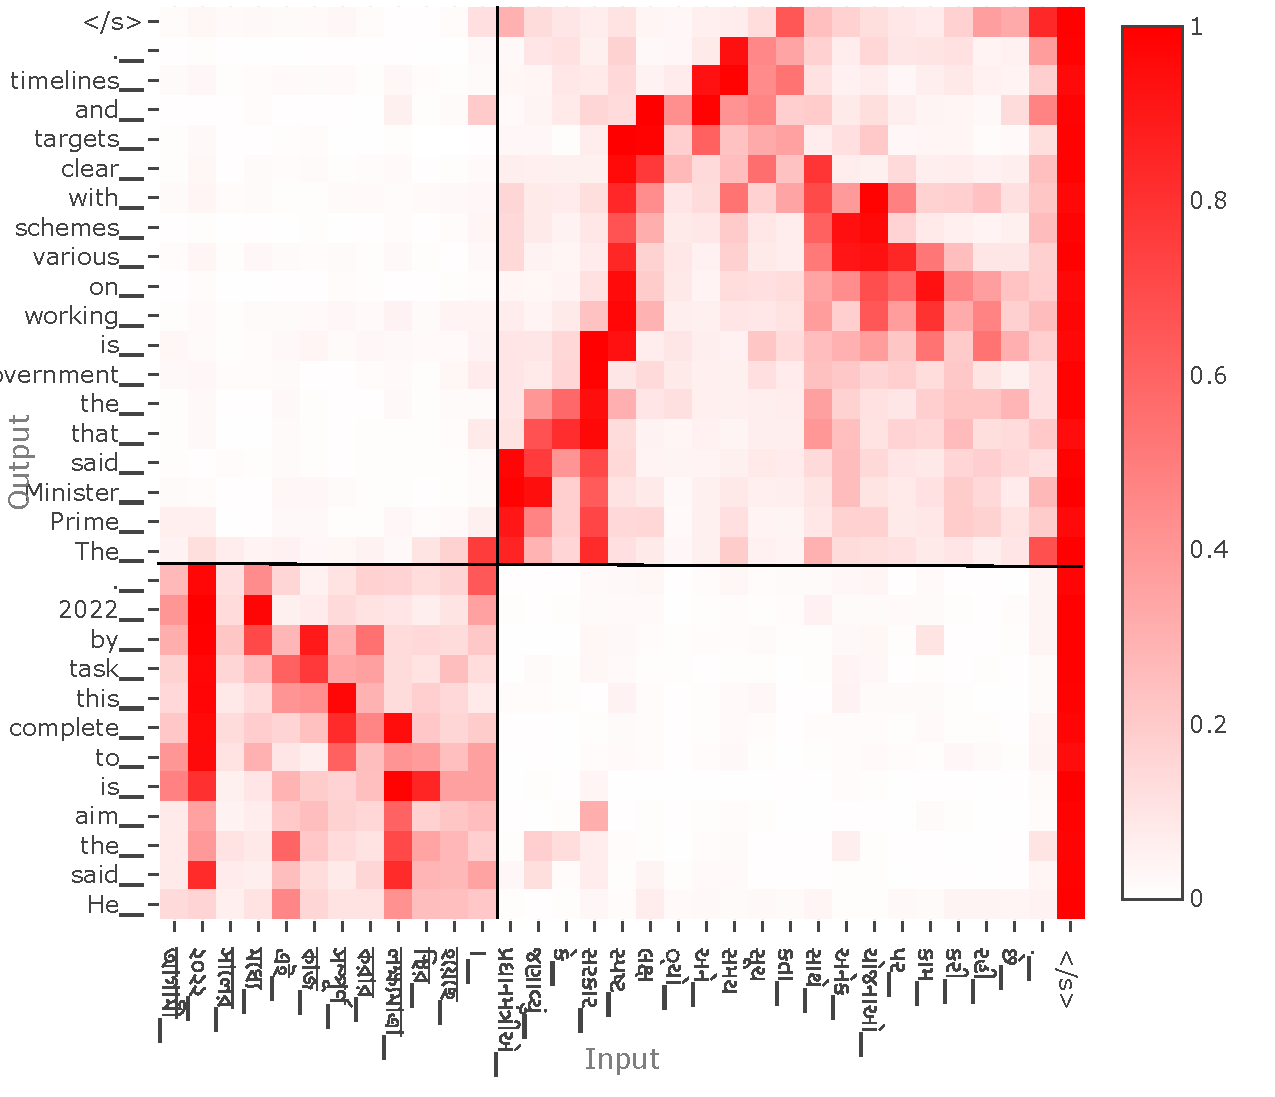
\includegraphics[width=\linewidth,trim={0mm 3mm 38mm 2mm},clip]{img/robustness/xattn-catXL-catXL+denoise-ann.pdf}
         \caption{Model trained with both CatXL and DenoiseTgt augmentations (\#A7)}
         \label{fig:denoise+catXL-on-catXL}
      \end{subfigure}
      
    \caption[Cross-attention visualization from baseline model and concatenated (cross-language) model.]{Cross-attention visualization from baseline model and concatenated (cross-language) model.
     For each position in the grid, only the maximum value across all attention-heads from all the layers is visualized. The darker color implies more attention weight, and the black bars indicate sentence boundaries. The model trained on concatenated sentences has more pronounced cross-attention boundaries than the baseline, indicating less mass is bled across sentences.
     The model trained on both concatenated and denoising sentences has the least attention mass across sentences.}
\label{fig:attnviz-catXL}
\end{figure}

\begin{comment}

\begin{figure}[h!t]
    \centering
    \begin{subfigure}[b]{0.49\linewidth}
         \centering
         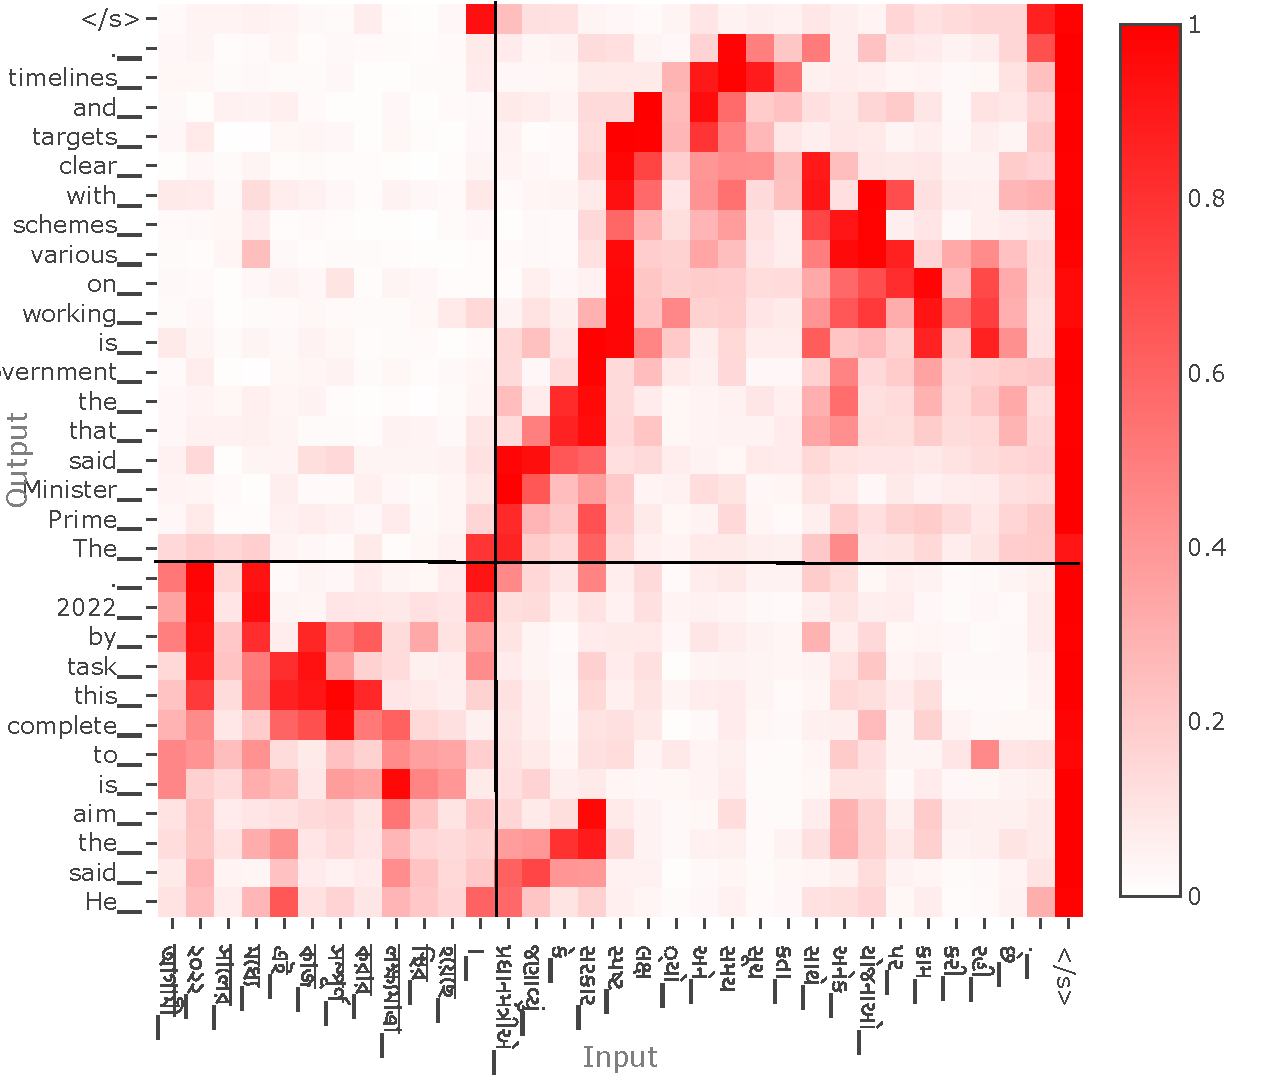
\includegraphics[width=\linewidth,trim={0mm 3mm 38mm 2mm},clip]{img/robustness/xattn-catXL-denoise-ann.pdf}
         \caption{Model trained with DenoiseTgt augmentation (\#A6)}
         \label{fig:denoise-on-catXL}
      \end{subfigure}
     \begin{subfigure}[b]{0.49\linewidth}
         \centering
         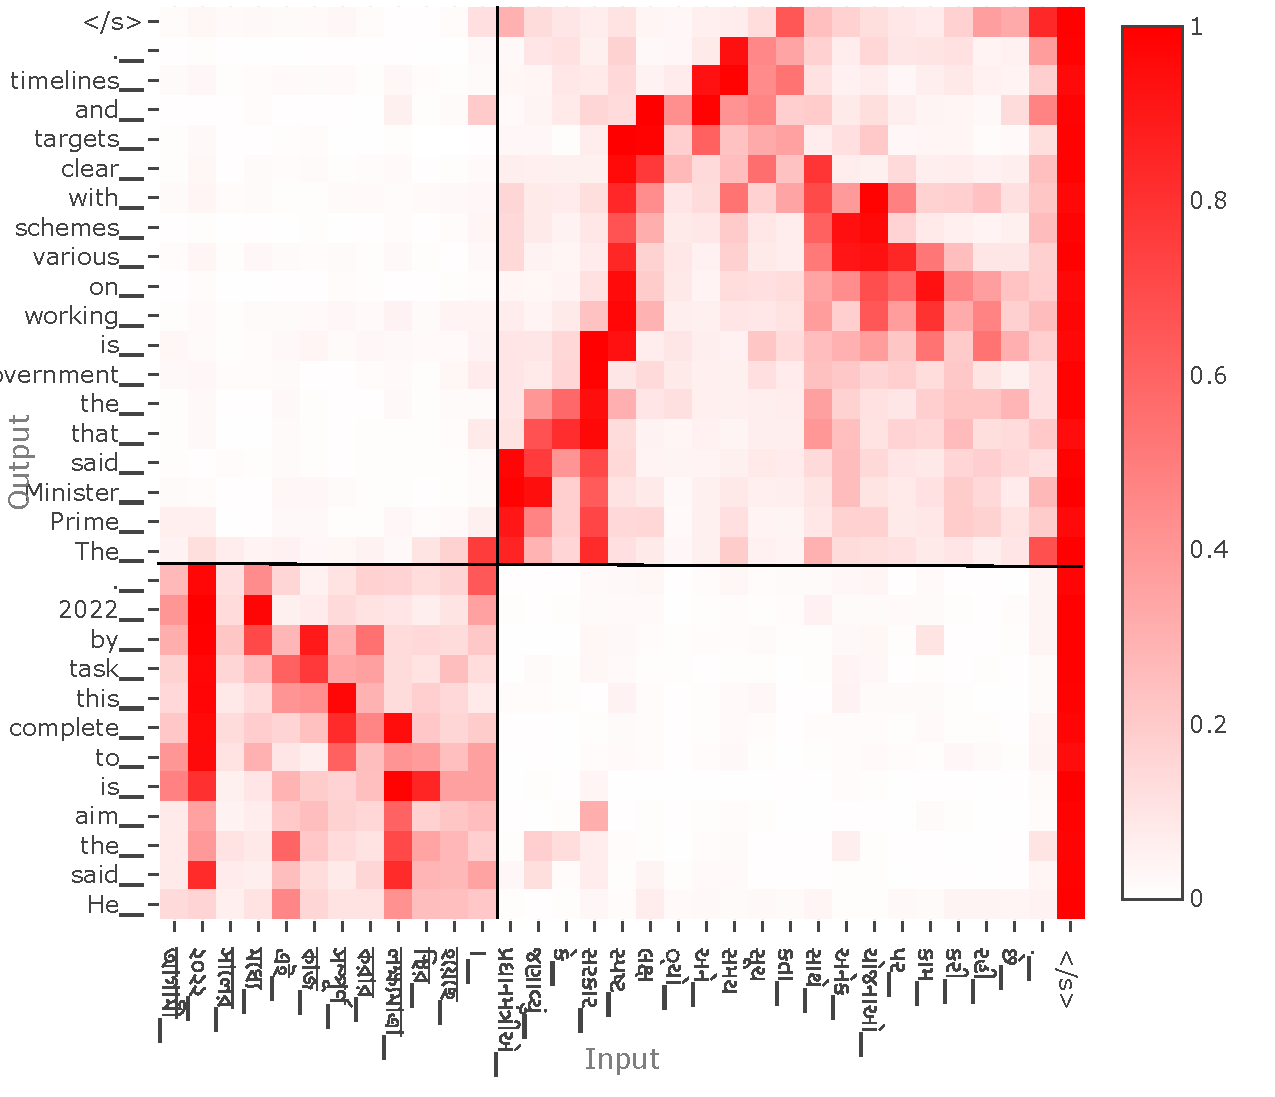
\includegraphics[width=\linewidth,trim={0mm 3mm 38mm 2mm},clip]{img/robustness/xattn-catXL-catXL+denoise-ann.pdf}
         \caption{Model trained with both CatXL and DenoiseTgt augmentations (\#A7)}
         \label{fig:denoise+catXL-on-catXL}
      \end{subfigure}
    \caption{Cross-attention visualization (... continuation from Figure~\ref{fig:attnviz-catXL}) The model trained on both concatenated and denoising sentences has least attention mass across sentences.}
    \label{fig:attnviz-catXL+denoise}
\end{figure}
\end{comment}
% test SVG support; oops fonts for unicodes are not supported
%\begin{figure}[htbp]
%  \centering
%  \includesvg[width=\linewidth]{tmp.svg}
%  \caption{svg image}
%\end{figure}


\subsection{Sentence Concatenation Generalization}
\label{sec:generalization}
In the previous sections, only two-segment concatenation has been explored; here, we investigate whether more concatenation further improves model performance and whether models trained on two segments generalize to more than two at test time.
We prepare a training dataset having up to four sentence concatenations and evaluate on datasets having up to four sentences.
As shown in Table~\ref{tab:cat-gen-bleus}, the model trained with just two segment concatenation achieves a similar BLEU as the model trained with up to four concatenations.
\begin{table}[ht]
\centering
\begin{tabular}{l rr : rr}
\hline
&\multicolumn{2}{c}{\textbf{Dev}} & \multicolumn{2}{c}{\textbf{Test}} \\
& C-SL & C-4SL & C-SL & C-4SL \\
\hline
Baseline / no join & 30.0 & 27.8 & 27.8 & 25.7 \\
Up to two joins & 31.9 & 28.9 & 29.7 & 26.7\\
Up to four joins & 31.0 & 28.9 & 28.8 & 26.8\\
\hline
\end{tabular} 
\caption{Indic$\shortarrow$English BLEU on held out sets containing up to 4 consecutive sentence concatenations in same language (C-4SL).
The two sentences dataset (C-SL) is also given for comparison.
The model trained on two concatenated sentences achieves comparable results on C-4SL, indicating that no further gains are obtained from increasing concatenation in training.}
\label{tab:cat-gen-bleus}
\end{table}


\section{Conclusion}

% We have investigated robustness of multilingual NMT and a few simple techniques to improve it.
We have described simple but effective checks for improving test coverage in multilingual NMT (Section~\ref{sec:multiling-mt-checks}), and have explored training data augmentation methods such as sentence concatenation and noise addition (Section~\ref{sec:train-aug}).
Using a many-to-one multilingual setup, we have investigated the relationship between these augmentation methods and their impact on robustness in multilingual translation. 
While the methods are useful in limited training data settings, their impact may not be visible on single-sentence test sets in a high resource setting. 
However, our proposed checklist evaluation reveals the robustness improvement in both the low resource and high resource settings.
We have conducted a glass-box analysis of cross-attention in Transformer NMT showing both visually and quantitatively that the models trained with augmentations, specifically, sentence concatenation and target sentence denoising, learn a more sharply focused attention mechanism (Section~\ref{sec:attn-bleed}).
Finally, we have determined that two-sentence concatenation in training corpora generalizes sufficiently to many-sentence concatenation inference (Section~\ref{sec:generalization}).  
%\section*{Acknowledgements}
%Thanks to 


\section*{Ethical Consideration}

%Machine translation is one of the very successful applications of natural language processing technologies, enabling communication across the language barriers.
%In this work we focus on a small subset of languages.

\paragraph{Limitations:} As mentioned in Section~\ref{sec:multiling-mt-checks}, some multilingual evaluation checks require the datasets to have multi-parallelism, and coherency in the sentence order.
When neither multi-parallelism nor coherency in the held-out set sentence order is available, we recommend R-XL. 
The data augmentation methods proposed in this paper do not require any specialized hardware or software.
Our model and training pipeline can be rerun on a variety of GPU models, including one with less memory, as 12 GB. 
However, some large dataset and large vocabulary models may require multiple distributed training processes, and/or multiple gradient accumulation steps to achieve the described batch size.

%\paragraph{Scientific Artifacts:} The experiments described in this chapter uses a dataset from The Workshop on Asian Translation 2021 (WAT21)'s \textit{MultiIndicMT} shared task~\cite{nakazawa-etal-2021-overview}, which is available for free download at the public URL: \url{http://lotus.kuee.kyoto-u.ac.jp/WAT/indic-multilingual/}; we do not redistribute this dataset from our servers.
%Our NMT pipeline is already publicly available under a license approved by \url{https://opensource.org}. Our code and scripts used for data preparation, augmentation, as well as model training and evaluation will be made available via a public GitHub repository with an open source-friendly license after the end of the author anonymity period. 

Only a subset of checks on robustness in multilingual settings have been discussed. While they serve as starting points for improving robustness, we do not claim that the proposed checks are exhaustive.
We have investigated robustness under Indic-English translation task where all languages use space characters as word-breakers; we have not investigated other languages such as Chinese, Japanese etc.
The term \textit{Indic} language to collectively reference 10 Indian languages only, similar to \textit{MultiIndicMT} shared task. While the remaining Indian languages and their dialects are not covered, 
we believe that the approaches discussed in this chapter generalize to other languages in the same family.


 \chapter{Rare Languages}
\label{ch:rare-langs}



\setlength{\epigraphwidth}{5.6in} 
\epigraph{\textit{``Vasudhaiva Kutumbakam" (The entire world is a family) } --- Maha Upanishad }



%Neural machine translation (NMT)~\cite{bahdanau2014nmtattn,vaswani-2017-attention} 
NMT has progressed to reach human performance on select benchmark tasks~\cite{barrault-etal-2019-findings,barrault-etal-2020-findings}. 
However, as MT research has mainly focused on translation between a few high resource languages, the unavailability of usable-quality translation models for low resource languages remains an ongoing concern.
Even those commercial translation services attempting to broaden their language coverage has only reached around one hundred languages; this excludes most of the thousands of languages used around the world today.

Freely available corpora of parallel data for many languages are available, though they are hosted at various sites, and are in various forms. A challenge for incorporating more languages into MT models is a lack of easy access to all of these datasets. While standards like ISO 639-3 have been established to bring consistency to the labeling of language resources, these are not yet widely adopted.
In addition, scaling experimentation to several hundred languages on large corpora involves a significant engineering effort.
Simple tasks such as dataset preparation, vocabulary creation, transformation of sentences into sequences, and training data selection becomes formidable at scale due to corpus size and heterogeneity of data sources and file formats.
We have developed tools to precisely address all these challenges, which we demonstrate in this work.
 
Specifically, we offer three tools which can be used either independently or in combination to advance NMT research on a wider set of languages (Section \ref{sec:tools}): firstly, \mtdata, which helps to easily obtain parallel datasets (Section \ref{sec:mtdata}); secondly, \nlcodec, a vocabulary manager and storage layer for transforming sentences to integer sequences, that is efficient and scalable (Section \ref{sec:nlcodec}); and lastly, \rtg, a feature-rich PyTorch-backed NMT toolkit that supports reproducible experiments (Section \ref{sec:rtg}).

We demonstrate the capabilities of our tools by preparing a massive bitext dataset with more than 9 billion tokens per side, and training a single multilingual NMT model capable of translating 500 source languages to English (Section \ref{sec:500-eng}).
We show that the multilingual model is usable either as a service for translating several hundred languages to English (Section \ref{sec:value.off-shelf-mt}), or as a parent model in a transfer learning setting for improving translation of low resource languages~(Section~\ref{sec:value.transfer-learning}). 
%pretrained multilingual embeddings (Section \ref{sec:value.embeddings}),


\section{Tools}
\label{sec:tools}
 Our tools are organized into the following sections:

\begin{comment}
Specifically, \textsc{MTData} (Section \ref{sec:mtdata}) is useful for preparing training data for hundreds of languages, 
\textsc{NLCodec} (section \ref{sec:nlcodec}) is useful for efficiently preprocessing, storing, and accessing the training data,
and \textsc{RTG} (section \ref{sec:rtg}) NMT toolkit for training an MT model. 
In addition, all these tools are built with reproducibility and usability in mind. 
These tools have been made publicly available, with permissive open source licenses.
We hope these tools help advance MT efforts beyond the top few high resource languages. 
\end{comment}

\subsection{\textsc{MTData}}
\label{sec:mtdata}
\textsc{MTData} addresses an important yet often overlooked challenge -- dataset preparation. 
By assigning an ID for datasets, we establish a clear way of communicating the exact datasets used for MT experiments, which helps in reproducing the experimental setup.
By offering a unified interface to datasets from many heterogeneous sources, \mtdata\ hides mundane tasks such as locating URLs, downloading, decompression, parsing, and sanity checking. Some noteworthy features are:
\begin{itemize}[noitemsep,topsep=0pt,leftmargin=4mm]
\item \textit{Indexer}: a large index of publicly available parallel datasets.
\item \textit{ID Standardization:} creates standardized IDs for datasets, along with language IDs normalized to BCP-47 like codes; more details in section \ref{sec:did-bcp47}. 
\item \textit{Parsers:} parses heterogeneous data formats for parallel datasets, and produces a simple plain text file by merging all the selected datasets.
\item \textit{Extensible:} new datasets and parsers can be easily added.
\item \textit{Local Cache}: reduces network transfers by maintaining a local cache, which is shared between experiments.
\item \textit{Sanity Checker}: performs basic sanity checks such as segment count matching and empty segment removal. When error states are detected, stops the setup with useful error messages.
\item \textit{Reproducible:} stores a signature file that can be used to recreate the dataset at a later time.
\item \textit{Courtesy:} shows the original \BibTeX\ citation attributed to datasets.
\item \textit{Easy Setup:} \texttt{pip install mtdata}
\item \textit{Open-source:} \url{https://github.com/thammegowda/mtdata}
\end{itemize}

Listing \ref{lst:mtdata-eg} shows an example for listing and getting datasets for German-English.
\begin{listing}
\begin{minted}[baselinestretch=1, fontsize=\normalsize, frame=lines, framesep=2mm,]{bash}
# List all the available datasets for deu-eng
$ mtdata list -l deu-eng
# Get the selected training & held-out sets
$ mtdata get -l deu-eng  -o data -ts Statmt-newstest_deen-201{8,9}-deu-eng \ 
  -tr Statmt-commoncrawl_wmt13-1-deu-eng Statmt-europarl-10-deu-eng \ 
      Statmt-news_commentary-16-deu-eng --merge
\end{minted}
\caption{\mtdata\ commands for listing and downloading German-English datasets (Tested on v0.3.4).
The \texttt{--merge} flag results in merging all the training datasets specified by \texttt{-tr} argument into a single file. }
\label{lst:mtdata-eg}
\end{listing}
 In Section~\ref{sec:datasets}, we use \mtdata to obtain thousands of publicly available datasets for a large many-to-English translation experiment.

\subsection{\nlcodec}
\label{sec:nlcodec}
\nlcodec\ is a vocabulary manager with encoding-decoding schemes to transform natural language sentences to and from integer sequences.\\
\textbf{Features:}
\begin{itemize}[noitemsep,topsep=0pt,leftmargin=4mm]
\item \textit{Versatile:} Supports commonly used vocabulary schemes such as characters, words, and byte-pair-encoding (BPE) subwords~\cite{sennrich-etal-2016-bpe}.
\item \textit{Scalable:} Apache Spark\footnote{\url{https://spark.apache.org/}}\cite{zaharia2016spark} backend can be optionally used to create a vocabulary from massive datasets.
\item \textit{Easy Setup:} \texttt{pip install nlcodec} 
\item \textit{Open-source:}\\ \url{https://github.com/isi-nlp/nlcodec/}
\end{itemize}

When the training datasets are too big to be kept in the primary random access memory (RAM), the use of secondary storage is inevitable.
The training processes requiring random examples lead to random access from a secondary storage device.
Even though the latest advancements in secondary storage technology such as solid-state drive (SSD) have faster serial reads and writes, their random access speeds are significantly lower than that of RAM. 
%In addition, since sentences are of variable lengths, use of fixed sized tensors are not feasible. 
To address these problems, we include an efficient storage and retrieval layer, \nldb, which has the following features:
\begin{itemize}[noitemsep,topsep=0pt,leftmargin=4mm]
  \item \textit{Memory efficient} by adapting data types based on vocabulary size. For instance, encoding with vocabulary size less than 256 (such as characters) can be efficiently represented using 1-byte unsigned integers. Vocabularies with fewer than 65,536 types, such as might be generated when using subword models \cite{sennrich-etal-2016-bpe} require only 2-byte unsigned integers, and 4-byte unsigned integers are sufficient for vocabularies up to 4 billion types. 
As the default implementation of Python, CPython, uses 28 bytes for all integers, we accomplish this using NumPy~\cite{harris2020numpy}. This optimization makes it possible to hold a large chunk of training data in smaller RAM, enabling fast random access.
  \item \textit{Parallelizable:} Offers a multipart database by horizontal sharding that supports parallel writes (e.g., Apache Spark) and parallel reads (e.g., distributed training).
%  \item \textit{I/O efficient:} Reads and writes large blocks at once instead of multiple smaller chunks, thus taking advantage of faster serial reads and write speeds.
  \item Supports commonly used batching mechanisms, such as random batches with approximately-equal-length sequences.
\end{itemize}

\nldb\ has a minimal footprint and is part of the \nlcodec\ package.
In Section~\ref{sec:500-eng}, we take advantage of the scalability and efficiency aspects of \nlcodec\ and \nldb\ to process a large parallel dataset with 9 billion tokens on each side.


\subsection{\rtg}
\label{sec:rtg}
Reader translator generator (\rtg) is a neural machine translation (NMT) toolkit based on Pytorch~\cite{NEURIPS2019_Pytorch}. 
Notable features of \rtg\ are:
\begin{itemize}[noitemsep,topsep=0pt,leftmargin=4mm]
\item \textit{Reproducible:} All the required parameters of an experiment are included in a single YAML configuration file, which can be easily stored in a version control system such as \texttt{git} or shared with collaborators.
\item Implements Transformer~\cite{vaswani-2017-attention}, and recurrent neural networks (RNN) with cross-attention models ~\cite{bahdanau2014nmtattn,luong2015effectiveAttn}.
%cho2014GRU,hochreiter1997LSTM
\item Supports distributed training on multi-node multi-GPUs, gradient accumulation, and Float16 operations.
\item Integrated Tensorboard helps in visualizing training and validation losses. 
% shows training speed, estimated finish time on \texttt{tqdm} progress-bar. 
\item Supports weight sharing~\cite{press-wolf-2017-embeddings}, parent-child transfer~\cite{zoph-etal-2016-transfer}, beam decoding with length normalization~\cite{wu-etal-2016-GNMT}, early stopping, and checkpoint averaging. 
%, and transfer learning with selective layer weight freezing. 
\item Flexible vocabulary options with \nlcodec\ and \sentpiece~\cite{kudo-richardson-2018-sentencepiece} which can be either shared or separated between source and target languages.
\item \textit{Easy setup:} \texttt{pip install rtg}
%\item A CLI for running end-to-end experiments based on a YAML config file (\texttt{rtg-pipe}); also supports experiment forking and export (\texttt{rtg-fork}, \texttt{rtg-export}).
%\item In addition to CLI interface for translation generation (\texttt{rtg-decode}), web and REST interfaces are also supported (\texttt{rtg-serve}).
\item \textit{Open-source:} \url{https://isi-nlp.github.io/rtg/}
\end{itemize}

\begin{comment}
% [
%frame=lines,
%framesep=2mm,
% baselinestretch=1.1,
% fontsize=\footnotesize,
%linenos
%]{bash}
\begin{listing}[ht]
\scriptsize
%\tiny
\inputminted{yaml}{sample-conf.yml}
\caption{An example \textit{conf.yml} file from an RTG experiment.}
\end{listing}


\begin{table}[]
    \centering
    \footnotesize
    \begin{tabular}{l  l| r r}
        NMT & BPE Impl  & NewsTest18 & NewsTest19 \\ \hline \hline
        \rtg & \nlcodec\   & 32.6   & 29.0 \\
        \rtg & \scriptsize{\sentpiece\ }& 32.3 & 28.7 \\
        FairSeq & subword-nmt & & \\
        T2T &  (built-in) & &
    \end{tabular}
    \caption{Transformer-base model is trained on the datasets shown in Listing~\ref{lst:mtdata-eg} for 200K optimizer updates having a batch size of 4200 tokens. All models use shared 8000 BPE subwords as vocabulary. The BLEU scores are from \sacrebleu\ \texttt{BLEU+c.mixed+l.de-en+\#.1+s.exp+t.wmt1\{8,9\}+tok.13a+v.1.4.13}.  }
    \label{tab:my_label}
\end{table}

\end{comment}

\section{Dataset ID Standardization}
\label{sec:did-bcp47}

Datasets collected from heterogeneous sources come in a variety of file formats, leading to chaos.  
We standardize parallel dataset IDs to the format:\footnote{Apache Maven uses a similar format for Java library IDs} $$\texttt{Group-Name-Version-Lang1-Lang2}$$
\begin{itemize}
    \item \textbf{Group}: Identifier of dataset origin, e.g., name of website or organization that has prepared the dataset.
    \item \textbf{Name}: Dataset name
    \item \textbf{Version}: Version number
    \item \textbf{Lang1} and \textbf{Lang2} are language IDs, which  are described in the following.
\end{itemize}

\textbf{Language ID standardization:} ISO 639-1\footnote{\url{https://www.iso.org/standard/4766.html}} is commonly used to identify languages in publications and software systems.  
This standard nomenclature uses two-letter codes, and has space for $26^2 = 676$ codes, out of which, only $183$ codes are officially assigned to languages. Thus, a vast majority of known, living languages do not have a standard identifier under ISO 639-1. 
On the other hand, \textbf{ISO 639-3}\footnote{\url{https://iso639-3.sil.org/}}, a revised but not yet widely adopted nomenclature, uses three-letter codes, and has space for $26^3 = 17,576$ languages with more than $7,800$ of them officially assigned. We have used ISO 639-3 since the early version of MTData.
However, we soon realized that ISO 639-3 does not distinguish nuances in languages. For instance, some users want to distinguish Brazilian Portuguese and Portuguese of Portugal, and have separate datasets created for these languages. 
The distinction between region and script variants of languages is not supported by ISO 639-3, and hence we have turned to Best Current Practice (BCP)-47 \cite{phillips2009bcp47} for resolving this problem.
BCP 47, also known as Internet Engineering Task Force (IETF) language tag, uses a combination of language, script, and region IDs to uniquely and consistently identify human languages.
This standard relies on the following other standards:
\begin{itemize}
    \item Language: ISO 639, e.g., \code{en, de, ils}
    \item Script: ISO 15924, e.g., \code{Latn, Cyrl}
    \item Region: ISO 3166-1  (e.g., \code{US, GB, IN, AU}), and UN M49 (e.g., \code{840, 826, 356, 036})
\end{itemize}

% BCP 47 is also been extended with advanced features such as transformations and locales. 
Since \mtdata{} version 0.3, we use a simplified BCP 47-like tags\footnote{Thanks, to Kenneth Heafield, for educating us with BCP 47.}. The implementation used in \mtdata{} matches BCP 47 specifications for the most part, except the following:
\begin{itemize}
    \item BCP 47 uses ISO 639-1 (i.e., two-letter code) for 183 languages and ISO 639-3 (i.e., three-letter codes) for the remaining languages. We use ISO 639-3 code for all languages. Our system, being relatively new, uses ISO 639-3 since the beginning, thus 639-3 is both consistent and backward compatible. 
    
    \item BCP 47 uses the `-' character to join languages, scripts, and region sub-tags. Since the MT community has long used `-' character to designate bitext languages, e.g., `\code{fra-eng}', we instead use `\_' character.
    
    \item For the region sub-tag, BCP 47 supports use of either the two-letter ISO 3166-1 codes, or the three digit UN M49 codes. We use ISO 3166-1 codes only, as it is the most popular and easy to comprehend.
    
    \item BCP 47 has support for tagging transformation as well as locale information. These are currently not supported in \mtdata{}, however these are interesting directions for future enhancements.
\end{itemize}

The script and region tags are optional. In favor of brevity, we suppress default scripts whenever unambiguous, e.g., \code{eng-Latn} is \code{eng} since \code{Latn} is the default script of English.

Therefore, with the above simplifications, our language tags are of the format: \code{aaa[\_Bbbb][\_CC]}, where (a) the mandatory three lowercase letters in the beginning is a valid language identifier from ISO 639-3 nomenclature, (b) the optional four letters (title-cased) in the middle is a script identifier from ISO 15924, and (c) the optional two upper-case letters in the end are region identifier from ISO 3166-1.

\section{Many-to-English Multilingual NMT}
\label{sec:500-eng}
In this section, we demonstrate the use of our tools by creating a massively multilingual NMT model from publicly available datasets. 

\subsection{Dataset}
\label{sec:datasets}
We use \mtdata\ to download datasets from various sources, given in Table~\ref{tab:data-sources}. 
To minimize data imbalance, we select only a subset of the datasets available for high resource languages, and select all available datasets for low resource languages. The selection is aimed to increase the diversity of data domains and quality of alignments. 

 \begin{table}[ht]
 \centering
 %\footnotesize
 \begin{tabular}{p{0.2\linewidth} p{0.5\linewidth}}
  Dataset   & Reference \\ \hline\hline
 Europarl    & \citet{koehn2005europarl} \\
 KFTT Ja-En & \citet{neubig11kftt}  \\ 
 Indian6     & \citet{post-etal-2012-constructing}   \\ 
 OPUS        & \citet{tiedemann-2012-parallel}  \\
 UNPCv1     & \citet{ziemski-etal-2016-unpc}   \\
 Tilde MODEL & \citet{rozis-skadins-2017-tilde}  \\
 TEDTalks    & \citet{qi-etal-2018-pretrainemb}  \\ 
 IITB Hi-En & \citet{kunchukuttan-etal-2018-iit} \\
 Paracrawl   & \citet{espla-etal-2019-paracrawl} \\
 WikiMatrix & \citet{schwenk-etal-2019-wikimatrixv1} \\
 JW300       & \citet{agic-vulic-2019-jw300}  \\
 PMIndia & \citet{haddow2020pmindia}  \\
 OPUS100    & \citet{zhang-etal-2020-multiling-nmt} \\
 WMT [13-20] & \citet{bojar-etal-2013-findings, bojar-etal-2014-findings, bojar-etal-2015-findings, bojar-etal-2016-findings, bojar-etal-2017-findings, bojar-etal-2018-findings, barrault-etal-2019-findings, barrault-etal-2020-findings} \\

 \end{tabular}
 \caption{Various sources of MT datasets.}
 \label{tab:data-sources}
\end{table}

\begin{figure}[ht]
    \centering
    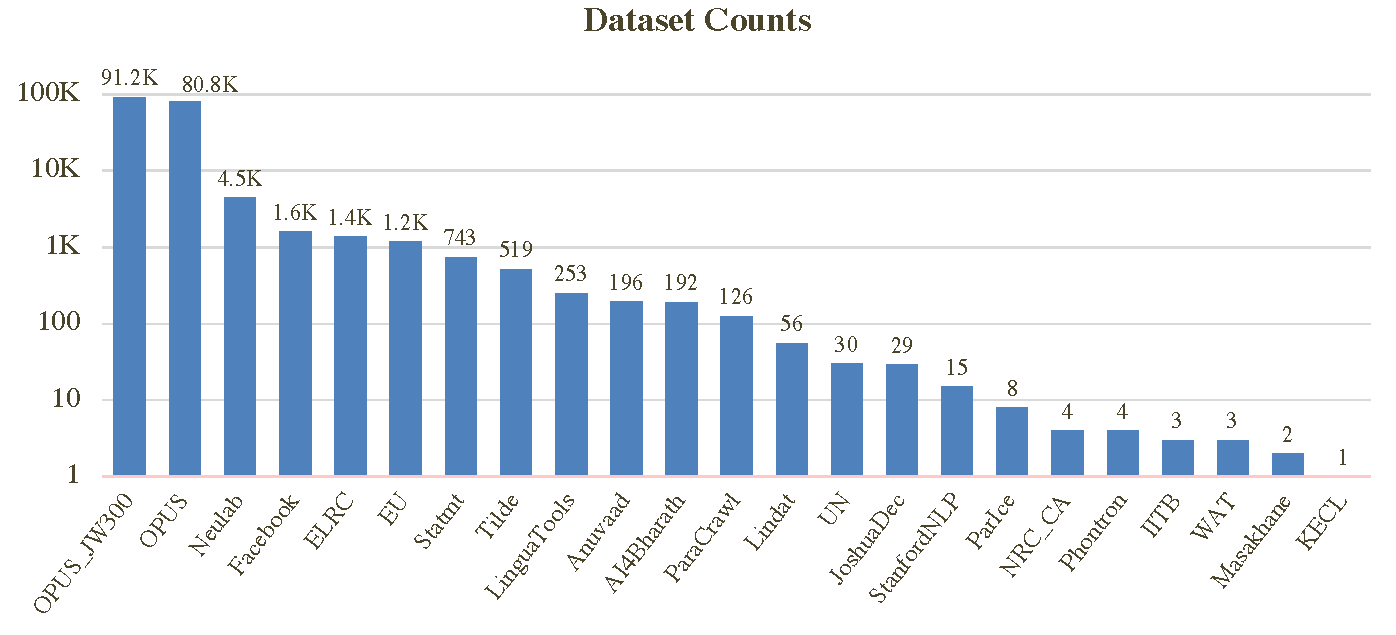
\includegraphics[width=\linewidth]{img/manyeng/mtdata-stats.pdf}
    \caption{Datasets curated from various sources. These statistics are extracted as of 2022 February (version 0.3.4)}.
    \label{fig:mtdata-stats}
\end{figure}


\begin{comment}
%\begin{figure*}[ht]
\begin{sidewaysfigure}
\centering
    %trim={5mm 4mm 5mm 5mm},clip
    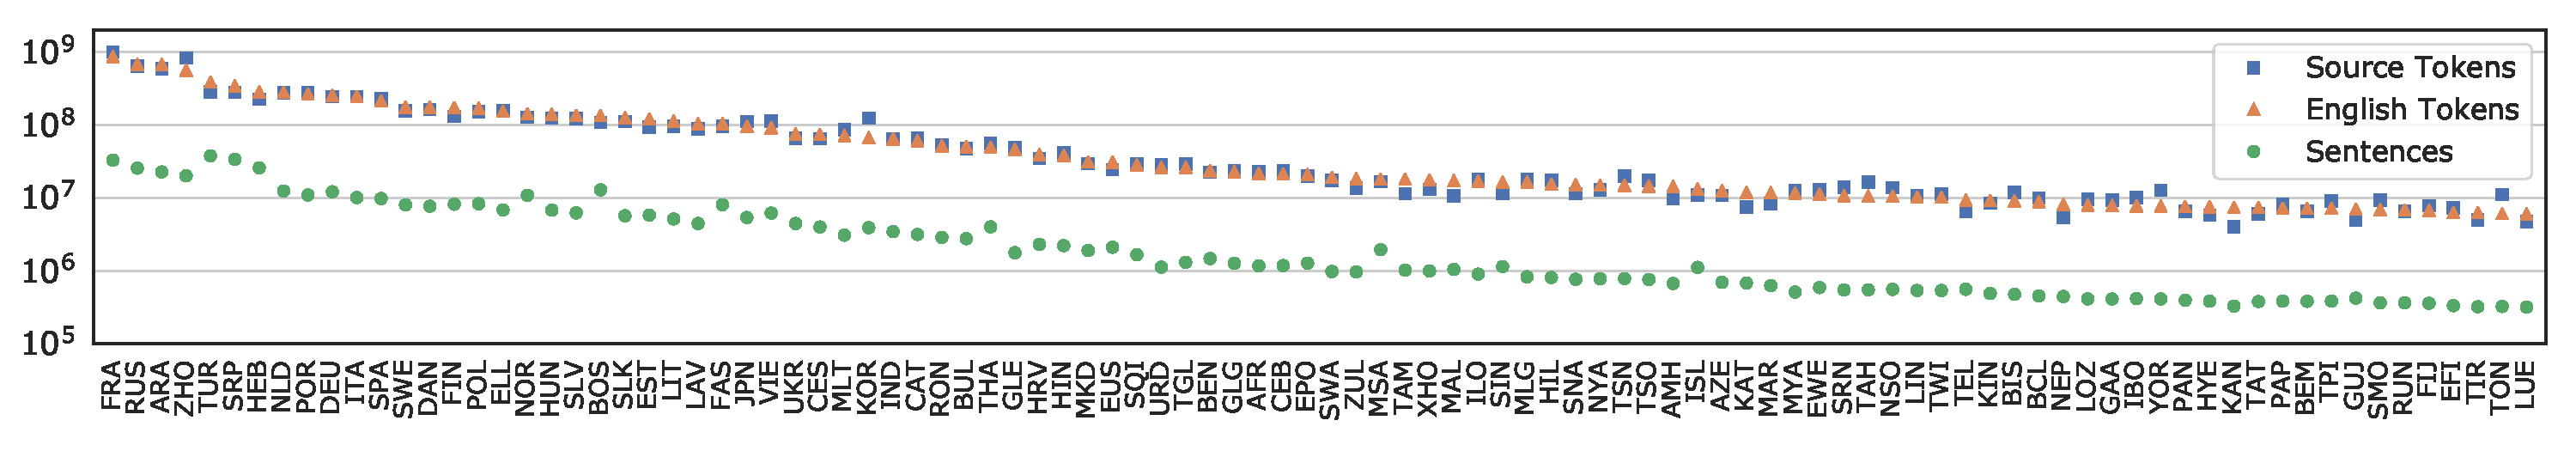
\includegraphics[height=0.14\vsize,trim={5mm 4mm 5mm 5mm},clip]{manyeng/lang-stats-1-100.pdf}
    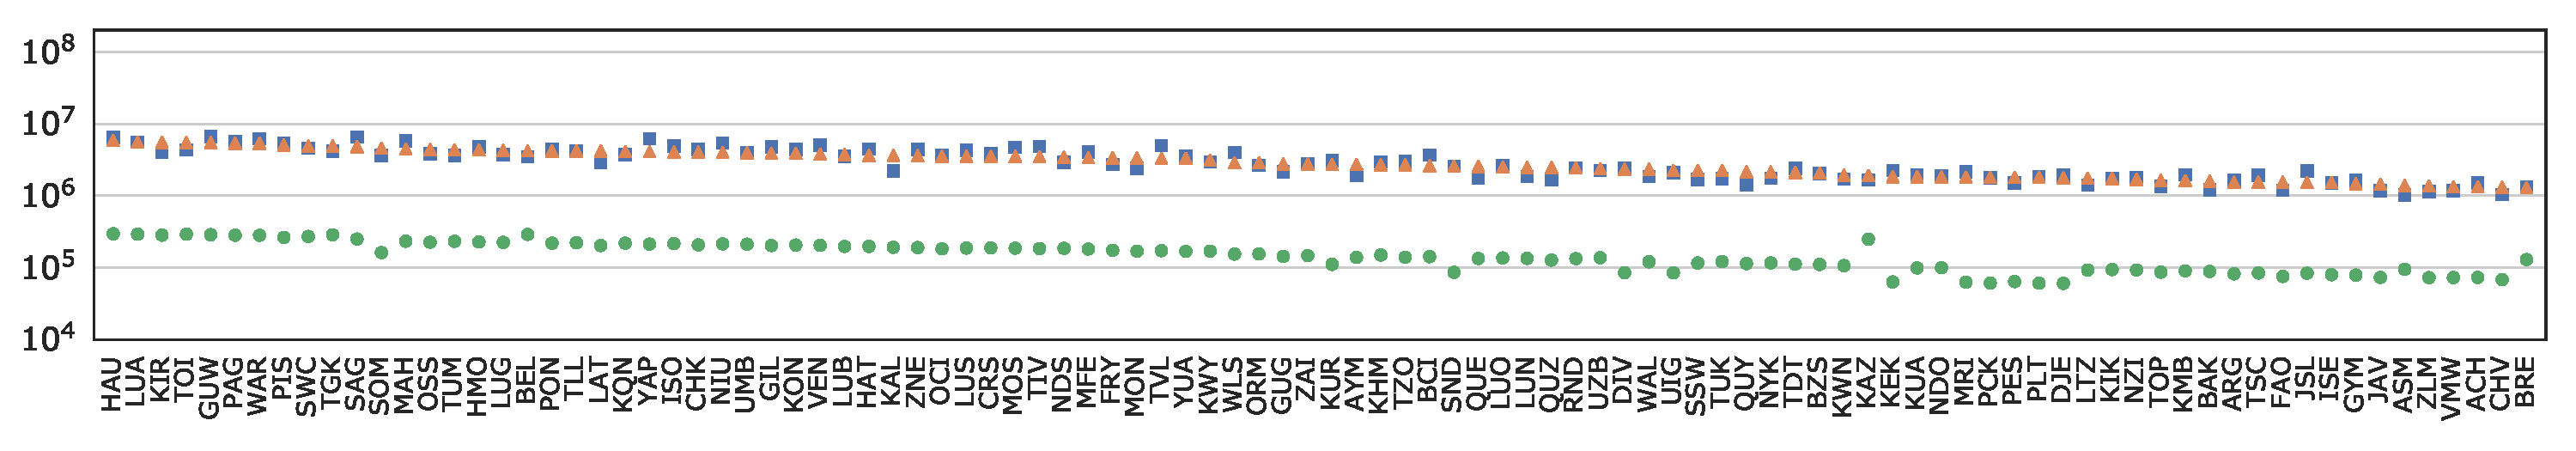
\includegraphics[height=0.14\vsize,trim={5mm 4mm 5mm 5mm},clip]{manyeng/lang-stats-101-200.pdf}
    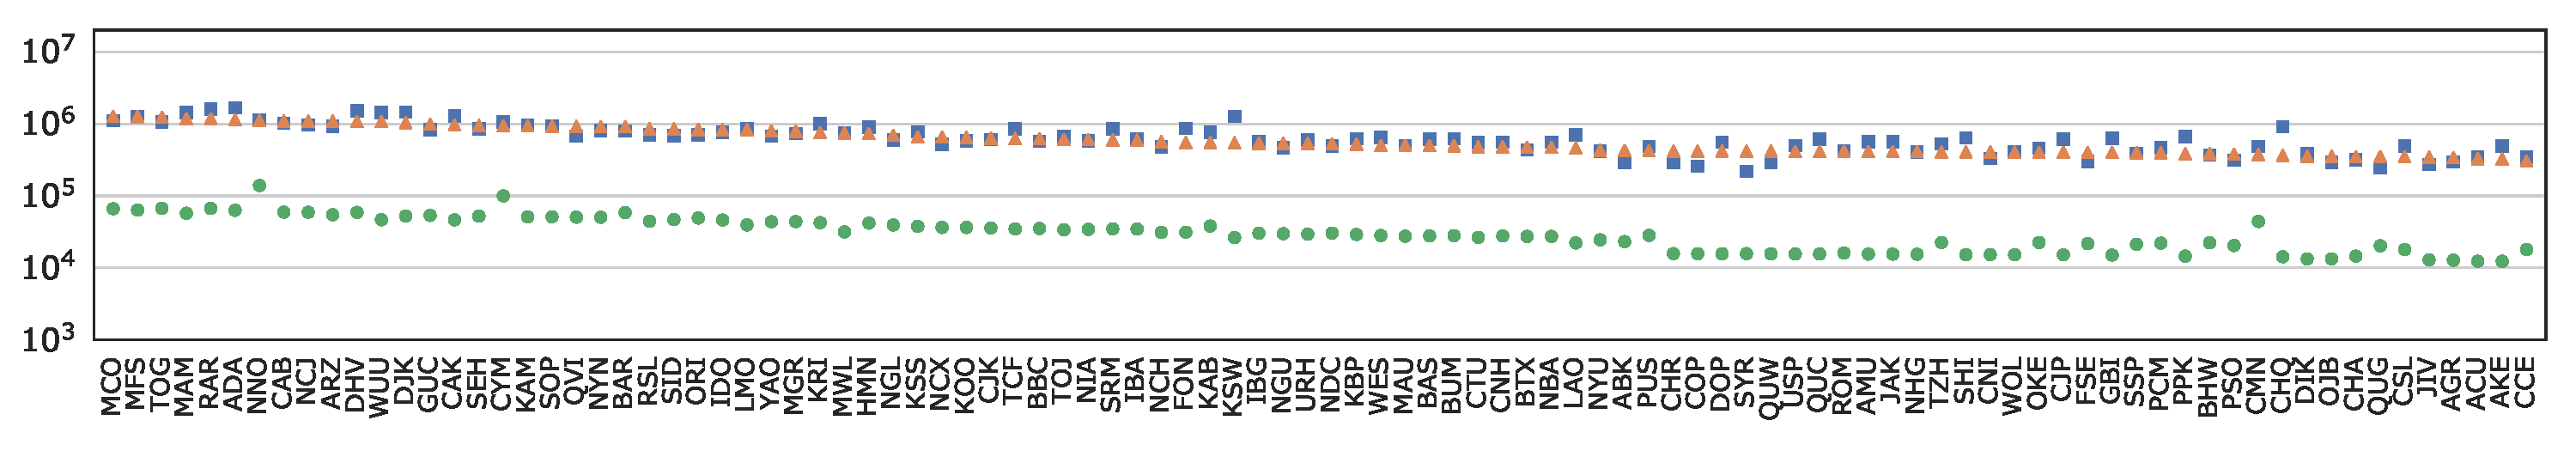
\includegraphics[height=0.14\vsize,trim={5mm 4mm 5mm 5mm},clip]{manyeng/lang-stats-201-300.pdf}
    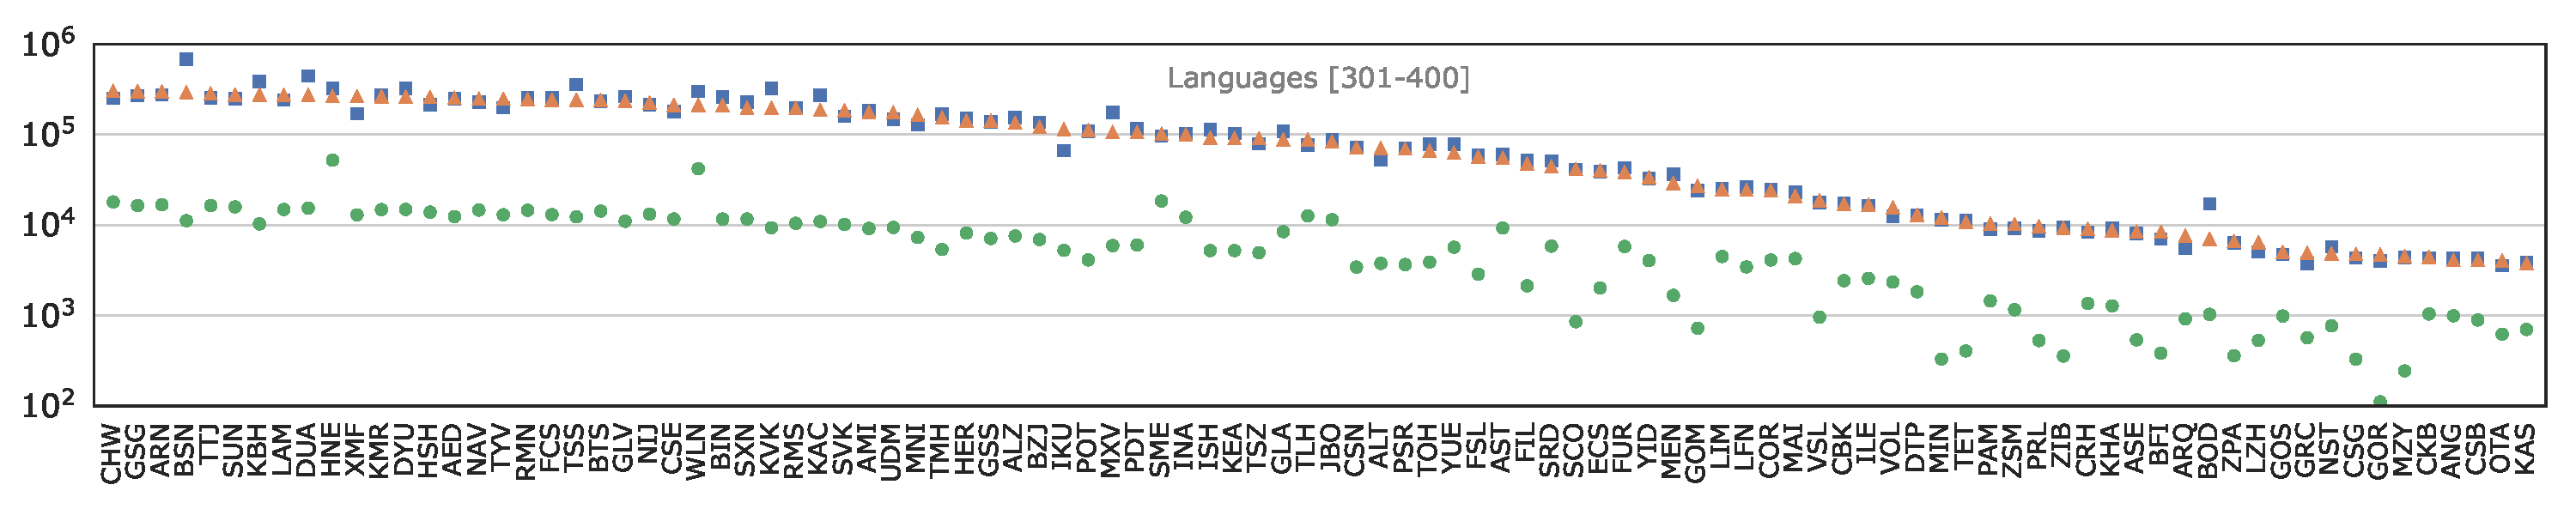
\includegraphics[height=0.14\vsize,trim={5mm 4mm 5mm 5mm},clip]{manyeng/lang-stats-301-400.pdf}
    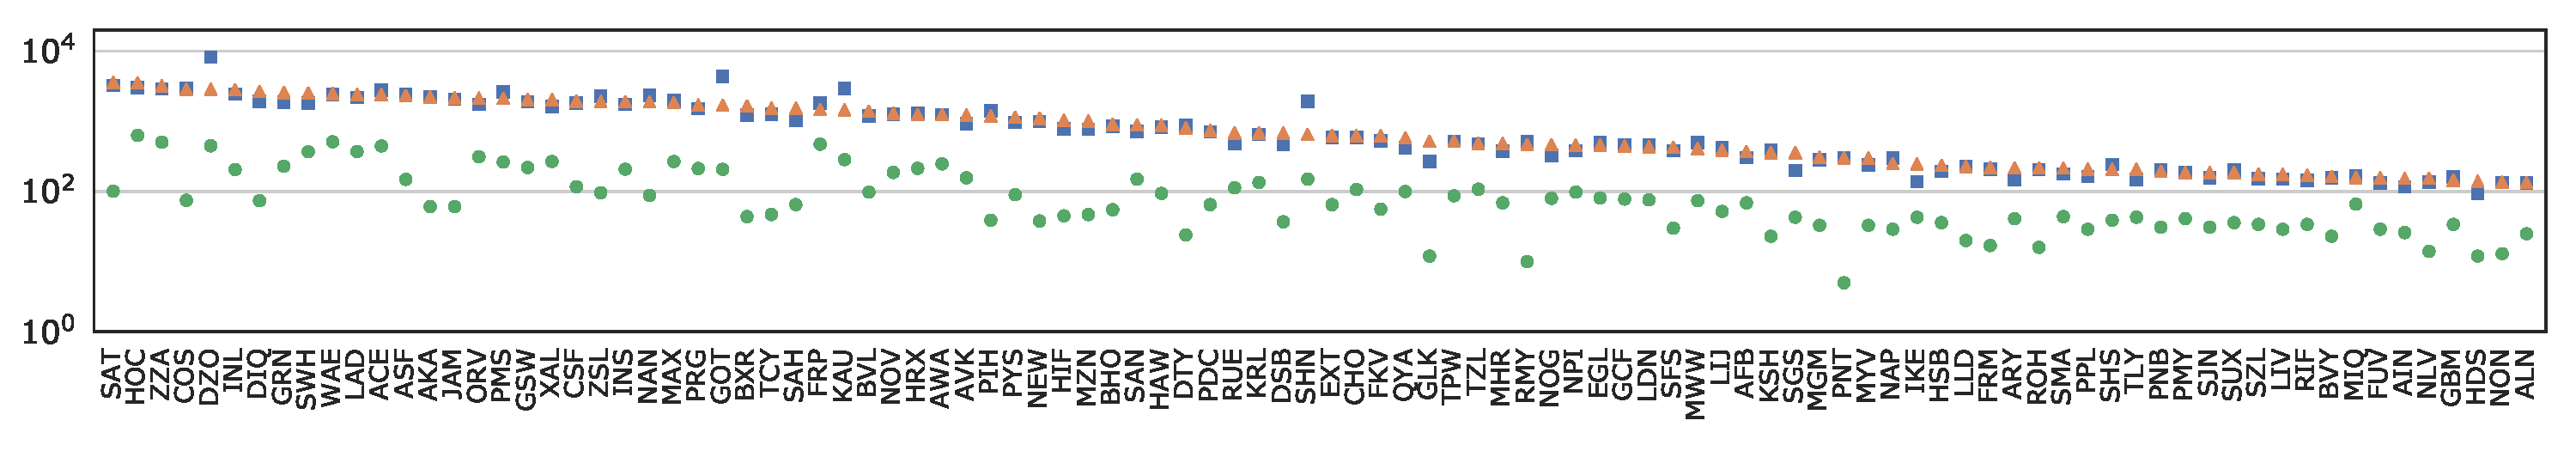
\includegraphics[height=0.14\vsize,trim={5mm 4mm 5mm 5mm},clip]{manyeng/lang-stats-401-500.pdf}     
    \caption{\centering Training data statistics for 500 languages, sorted as descending order of English token count,  obtained after de-duplication and filtering (see Section~\ref{sec:datasets}). The full name for these ISO 639-3 codes can be looked up using \mtdata, e.g. \texttt{mtdata-iso eng}. }
       \label{fig:train-data-stats}
\end{sidewaysfigure}
%\end{figure*}
\end{comment}

\begin{figure*}[h!t]
\centering
    %trim={5mm 4mm 5mm 5mm},clip
    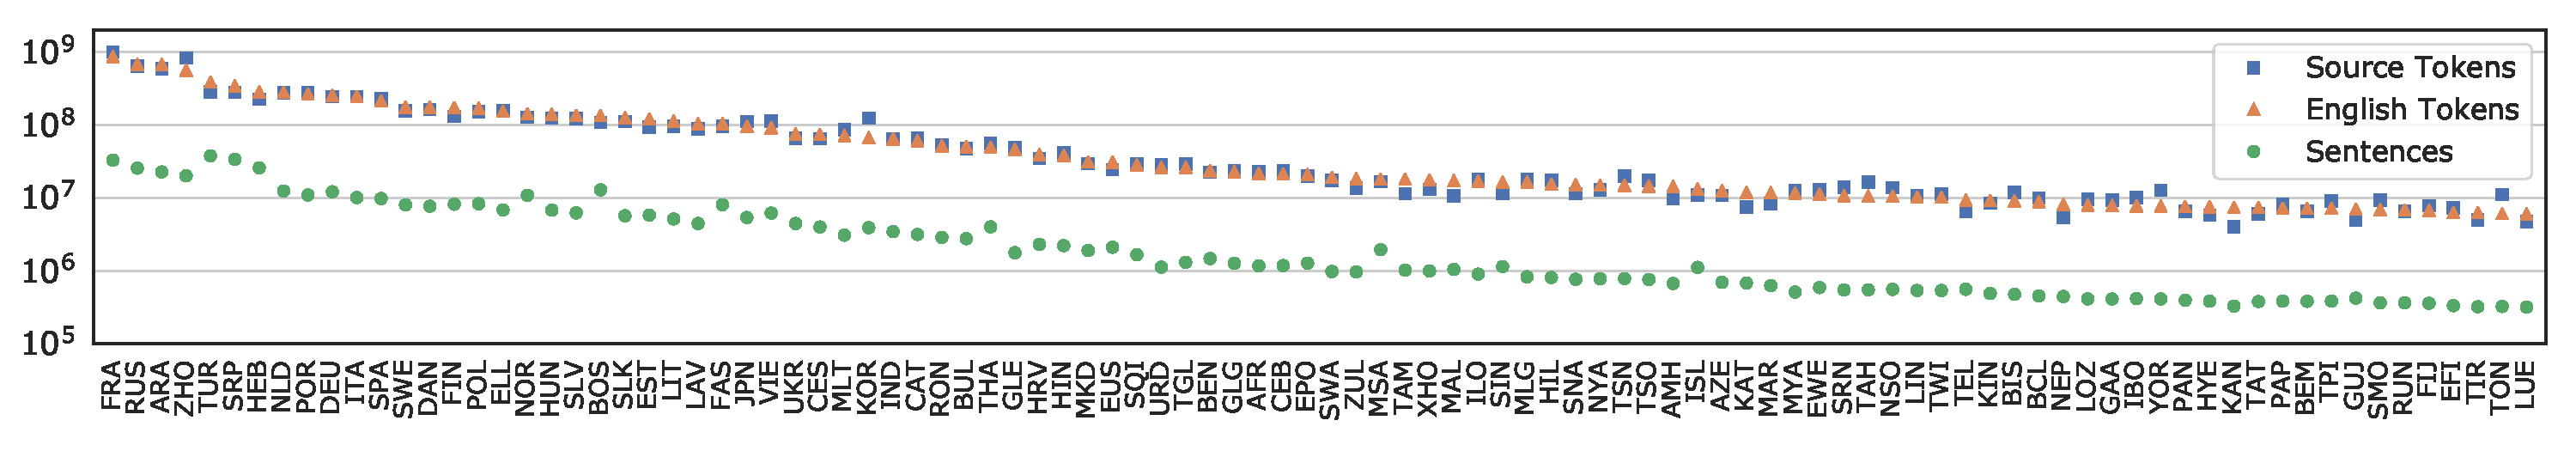
\includegraphics[width=\linewidth,trim={5mm 4mm 5mm 5mm},clip]{manyeng/lang-stats-1-100.pdf}
    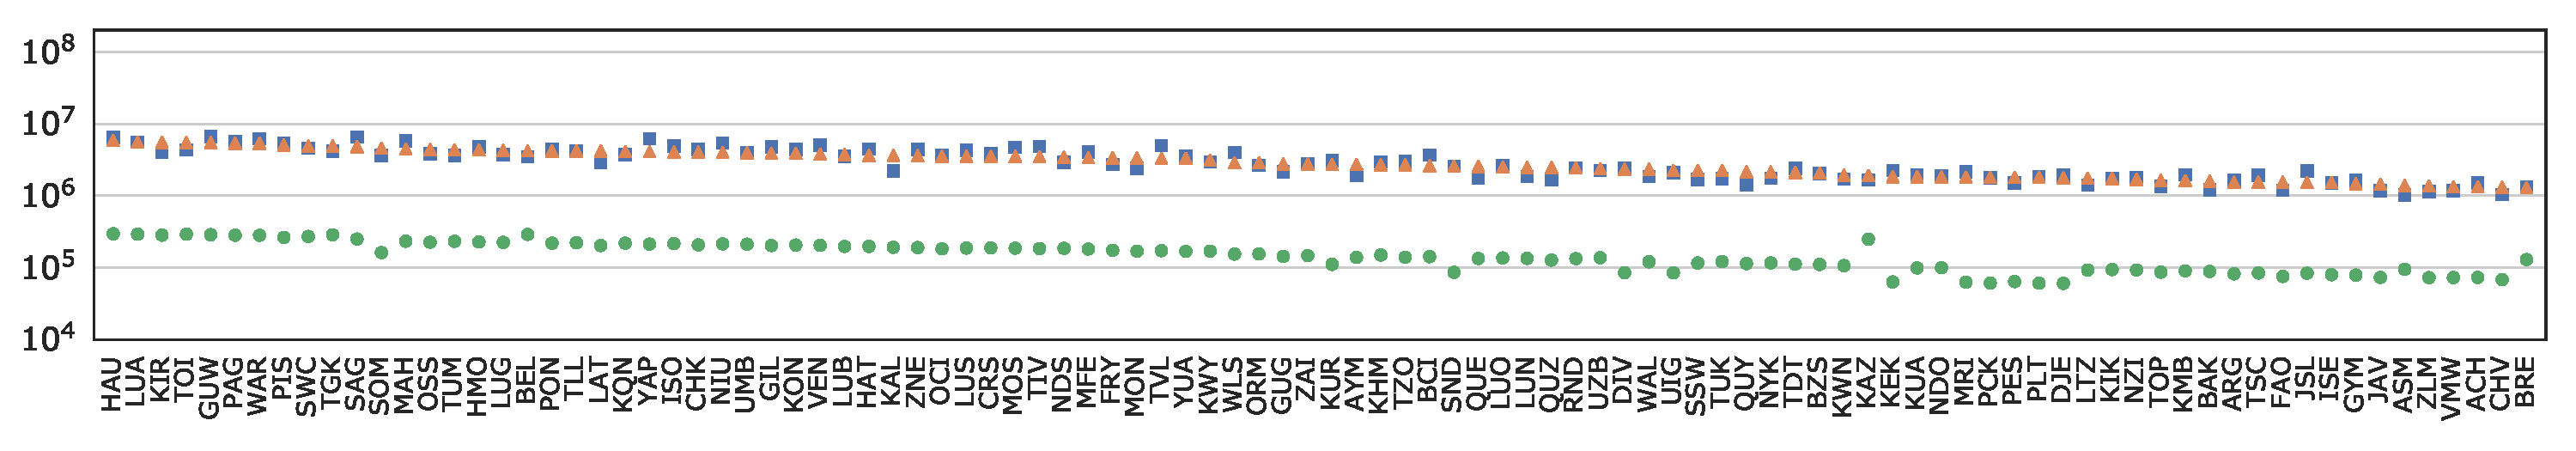
\includegraphics[width=\linewidth,trim={5mm 4mm 5mm 5mm},clip]{manyeng/lang-stats-101-200.pdf}
    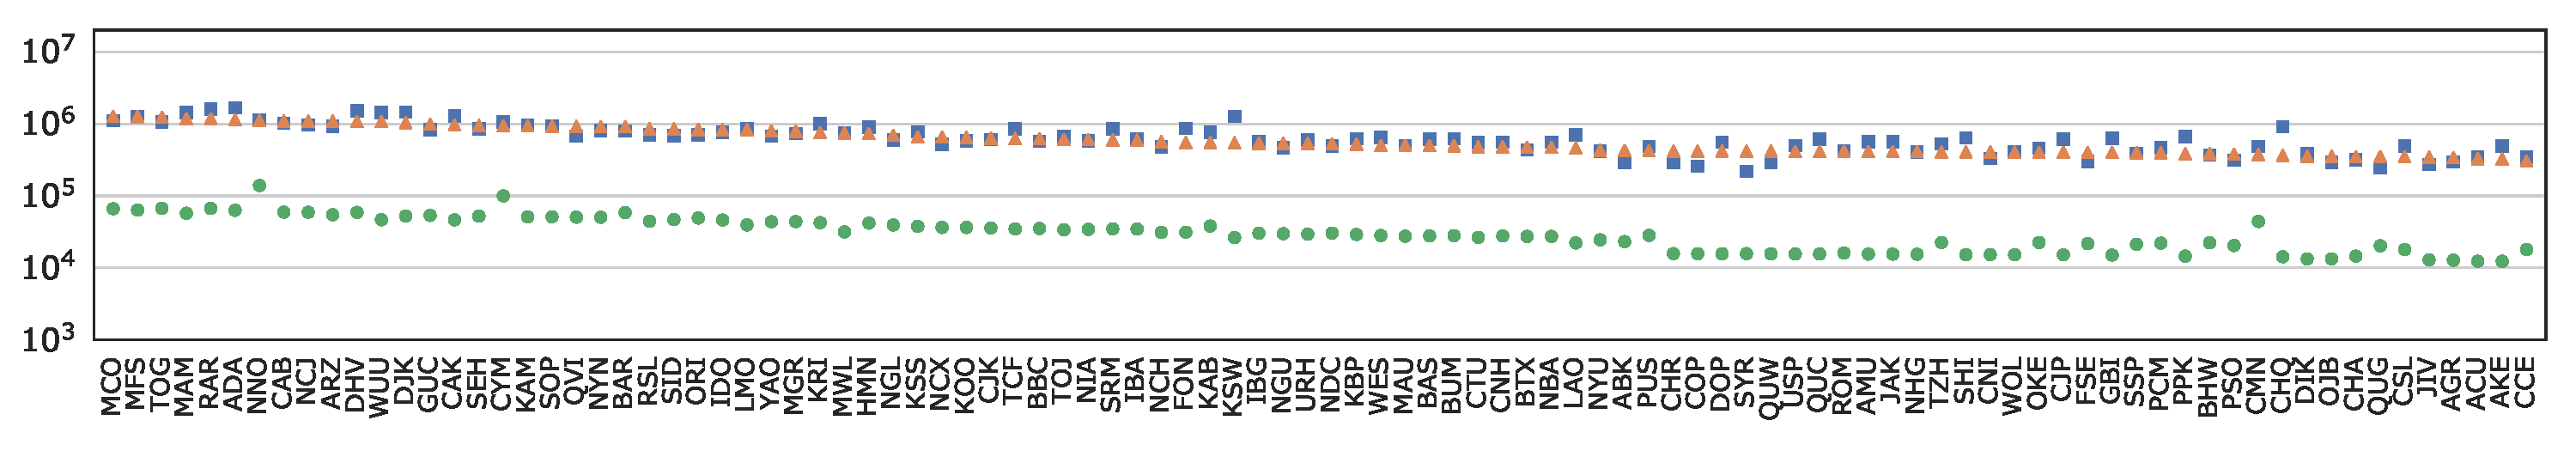
\includegraphics[width=\linewidth,trim={5mm 4mm 5mm 5mm},clip]{manyeng/lang-stats-201-300.pdf}
    \includegraphics[width=\linewidth,trim={5mm 4mm 5mm 5mm},clip]{manyeng/lang-stats-301-400.pdf}
    \includegraphics[width=\linewidth,trim={5mm 4mm 5mm 5mm},clip]{manyeng/lang-stats-401-500.pdf}     
    \caption{Training data statistics for 500 languages, sorted as descending order of English token count,  obtained after deduplication and filtering (see Section~\ref{sec:datasets}). The full name for these ISO 639-3 codes can be looked up using \mtdata, e.g. \texttt{mtdata-iso eng}.}
       \label{fig:train-data-stats}
\end{figure*}



\textbf{Cleaning:}
 We use \textsc{SacreMoses}\footnote{\url{https://github.com/isi-nlp/sacremoses} a fork of \url{https://github.com/alvations/sacremoses} with improvements to tokenization for many low resource languages.} to normalize Unicode punctuations and digits, followed by word tokenization. 
We remove records that are duplicates, have abnormal source-to-target length ratios, have many non-ASCII characters on the English side, have a URL, or which overlap exactly, either on the source or target side, with any sentences in held out sets.
As preprocessing is compute-intensive, we parallelize using Apache Spark.
The cleaning and tokenization results in a corpus of 474 million sentences and 9 billion tokens on the source and English sides each. The token and sentence count for each language are provided in Figure~\ref{fig:train-data-stats}.
Both the processed and raw datasets are available at \url{http://rtg.isi.edu/many-eng/data/v1/}.\footnote{A copy is at \url{https://opus.nlpl.eu/MT560.php}}

\subsection{Many-to-English Multilingual Model}
\label{sec:500eng-model}
We use \rtg\ to train Transformer NMT \cite{vaswani-2017-attention} with a few modifications.
Firstly, instead of a shared BPE vocabulary for both source and target, we use two separate BPE vocabularies. 
Since the source side has 500 languages and the target side has English only, we use a large source vocabulary and a relatively smaller target vocabulary.
A larger target vocabulary leads to higher time and memory complexity, whereas a large source vocabulary increases only the memory complexity but not the time complexity.
We train several models, ranging from the standard 6 layers, 512-dimensional Transformers to larger ones with more parameters. Since the dataset is massive, a larger model trained on big mini-batches yields the best results. Our best performing model is a 768 dimensional model with 12 attention heads, 9 encoder layers, 6 decoder layers, feed-forward dimension of 2048, dropout and label smoothing at 0.1, using $512,000$ and $64,000$ BPE types as source and target vocabularies, respectively. The decoder's input and output embeddings are shared.
Since some English sentences are replicated to align with many sentences from different languages (e.g. the Bible corpus), BPE merges are learned from the deduplicated sentences using \nlcodec.
Our best performing model is trained with an effective batch size of about 720,000 tokens per optimizer step. Such big batches are achieved by using mixed-precision distributed training on 8 NVIDIA A100 GPUs with gradient accumulation of 5 mini-batches, each having a maximum of 18,000 tokens. We use the Adam optimizer~\cite{kingma2015adam} with 8000 warm-up steps followed by a decaying learning rate, similar to \citet{vaswani-2017-attention}. 
We stop training after five days and six hours when a total of 200K updates are made by the optimizer; validation loss is still decreasing at this point. 
To assess the translation quality of our model, we report BLEU~\cite{papineni-etal-2002-bleu,post-2018-sacrebleu}\footnote{All our BLEU scores are obtained from \sacrebleu\ \texttt{BLEU+c.mixed+\#.1+s.exp+tok.13a+v.1.4.13}.} on a subset of languages for which known test sets are available, as given in Figure~\ref{fig:test-bleu}, along with a comparison to \citet{zhang-etal-2020-multiling-nmt}'s best model.\footnote{
%a multilingual 24-layered 512-dimensional Transformer model having Merged Attention, Language-aware Layer Normalization and Linear Transformation, and trained including random online backtranslation.
Scores are obtained from \url{https://github.com/bzhangGo/zero/tree/master/docs/multilingual_laln_lalt}; accessed: 2021/03/30}

\begin{figure*}[ht]
    \centering
    \includegraphics[width=1\textwidth]{manyeng/BLEU-opus100.pdf}
    \caption[Many-to-English model's BLEU scores on OPUS-100 test set]{Many-to-English BLEU on OPUS-100 tests~\cite{zhang-etal-2020-multiling-nmt}. 
    Despite having four times more languages on the source side, our model scores competitive BLEU on most languages with the strongest system of \citet{zhang-etal-2020-multiling-nmt}. The tests where our model scores lower BLEU have shorter source sentences (mean length of about three tokens).}
    \label{fig:test-bleu}
\end{figure*}
%All BLEU scores are mixed-cased and are obtained using the default settings of \sacrebleu.
% https://github.com/bzhangGo/zero/tree/master/docs/multilingual_laln_lalt

\begin{comment}
\begin{subfigure}[t]{0.68\textwidth}
        \centering
        \includegraphics[width=\linewidth]{manyeng/BLEU-nttalksv1.pdf}
        %\caption{Lorem ipsum}
    \end{subfigure}%
    ~ 
    \begin{subfigure}[t]{0.31\textwidth}
        \centering
        \includegraphics[width=\linewidth,trim={7mm 0mm 0mm 0mm},clip]{img/BLEU-wmt-etc.pdf}
        %\caption{Lorem ipsum}
    \end{subfigure}
     TED Talks~\cite{qi-etal-2018-pretrainemb}, WMT~\cite{barrault-etal-2019-findings}, UNv1~\cite{ziemski-etal-2016-unpc}, and Indian-6~\cite{post-etal-2012-constructing}.
\end{comment}



\section{Applications}
\label{sec:value}
The model we trained as a demonstration for our tools is useful on its own, as described in the following sections. 

\subsection{Readily Usable Translation Service}
\label{sec:value.off-shelf-mt}
Our pretrained NMT model is readily usable as a service capable of translating several hundred source languages to English.
By design, source language identification is not necessary.
Figure~\ref{fig:test-bleu} shows that the model scores more than 20 BLEU, which maybe be a useful quality for certain downstream applications involving web and social media content analysis.
Apache Tika \cite{mattmann2011tika}, a content detection and analysis toolkit capable of parsing thousands of file formats, has an option for translating any document into English using our multilingual NMT model.\footnote{\url{https://cwiki.apache.org/confluence/display/TIKA/NMT-RTG}} Our model has been packaged and published to DockerHub\footnote{\url{https://hub.docker.com/}}, which can be obtained by the following command:
\begin{minted}[
%frame=lines,
%framesep=2mm,
baselinestretch=1.1,
fontsize=\normalsize,
%linenos
]{bash}
docker run --rm -i -p 6060:6060 tgowda/rtg-model:500toEng-v1
# For GPU backend, add --gpus '"device=0"' 
\end{minted}

The above command starts a docker image with HTTP server having a web interface, as can be seen in Figure~\ref{fig:rtg-webui}, and a REST API.
An example interaction with the REST API is as follows: 
\begin{figure}[ht]
    \centering
    \includegraphics[width=0.8\linewidth,trim=20 60 100 15,clip]{manyeng/rtg-webui.png}
    \caption{RTG Web Interface}
    \label{fig:rtg-webui}
\end{figure}

\begin{minted}[baselinestretch=1.1, fontsize=\normalsize]{bash}
$ API="http://localhost:6060/translate"
$ curl --data "source=Comment allez-vous?" --data "source=Bonne journée" $API
\end{minted}

\begin{minted}[baselinestretch=1.1, fontsize=\normalsize]{json}
 { 
   "source": [ "Comment allez-vous?", "Bonne journée" ],
   "translation": [ "How are you?", "Have a nice day" ]
}
\end{minted}


\subsection{Parent Model for Low Resource MT}
\label{sec:value.transfer-learning}
%WMT 20 has two low resource languages: IU and KM http://statmt.org/wmt20/translation-task.html 
%Uyghur from Lorelei?  Pashto  from Material?
 Fine-tuning is a useful transfer learning technique for improving the translation of low resource languages ~\cite{zoph-etal-2016-transfer,neubig-hu-2018-rapid,gheini2019universal}. 
 In the following subsections, we explore fine-tuning in both bilingual and multilingual setups.
 
 \subsubsection{Bilingual Setup}
Consider Breton-English (bre-eng) and Northern Sami-English (sme-eng), two of the low resource settings for which our model has relatively low BLEU (see Figure~\ref{fig:test-bleu}). 
To show the utility of fine-tuning with our model, we train a strong baseline Transformer model, one for each language, from scratch using OPUS-100 training data~\cite{zhang-etal-2020-multiling-nmt}, and fine-tune our multilingual model on the same dataset as the baselines. We shrink the parent model vocabulary and embeddings to the child model dataset, and train all models on NVIDIA P100 GPUs until convergence.\footnote{More info: \url{https://github.com/thammegowda/006-many-to-eng/tree/master/lowres-xfer}}
 Table~\ref{tab:transfer-lowres}, which shows BLEU on the OPUS-100 test set for the two low resource languages, indicates that our multilingual NMT parent model can be further improved with fine-tuning on limited training data.
 The fine-tuned model achieves 10 \bleu{} higher than the baseline model.

\begin{table}[ht]
    \centering
    %\footnotesize
    \begin{tabular}{l  r r}
        Model     & bre-eng & sme-eng \\ \hline\hline
        Baseline  & 12.7  &  10.7  \\
        Parent    & 11.8  &  8.6  \\
        \textit{Finetuned} & \textbf{22.8}  & \textbf{19.1}  \\ 
    \end{tabular}
    \caption{Finetuning our multilingual NMT on limited training data in low resource settings significantly improves translation quality, as quantified by BLEU.}
    \label{tab:transfer-lowres}
\end{table}

\subsubsection{Multilingual Model}
In the previous section, the 500-English multilingual model was proven effective while independently adapting to each rare language, e.g., bre-eng and sme-eng. 
In this section, we explore joint adaptation simultaneously to 9 low resource languages, taken from IARPA MATERIAL program.\footnote{https://www.iarpa.gov/research-programs/material}.
Table~\ref{tab:material-lang-stats} provides training data statistics for all nine languages. 
See Table \ref{tab:material-scores} for the results.

\begin{table}[h!t]
\small
\centering
\begin{tabular}{l | rrr | rrr} 
\hline 
\multirow{2}{*}{ Languages } & \multicolumn{3}{c |}{Clean parallel} & \multicolumn{3}{c}{Noisy parallel} \\
& Sents & Source Toks & English Toks & Sents & Source Toks & English Toks \\ \hline \hline 
swa-eng & 72.3k & 1.8M & 2.0M & 498k & 12.6M & 14.8M \\
tgl-eng & 46.7k & 804k & 823k & 744k & 21.4M & 20.7M \\
som-eng & 21.5k & 651k & 688k & 4.8M & 124.0M & 126.3M \\
lit-eng & 39.5k & 655k & 857k & 3.0M & 64.1M & 76.0M \\
pus-eng & 39.9k & 886k & 820k & 1.05M & 14.2M & 12.9M \\
bul-eng & 38.1k & 773k & 858k & 11.1M & 282.4M & 295.2M \\
kat-eng & 3.3k & 52k & 74k & 3.5M & 59.0M & 76.1M \\
kaz-eng & 71.4k & 559k & 595k & 25.0M & 423M & 515.9M \\
fas-eng & 31.7k & 715k & 798k & 249k & 5.6M & 5.3M \\ \hdashline
Combined & 364.3k & 6.9M & 7.5M & 49.9M & 1.0B & 1.1B \\
\hline 
\end{tabular} 
\caption{Training data statistics for 9 low resource languages used in IARPA MATERIAL program.}
\label{tab:material-lang-stats}
\end{table}

%\vspace{6mm}

\begin{table}
\small 
\centering
    \begin{tabular}{l | rrrr | rrrr}
    \hline
& \multicolumn{4}{c|}{BLEU (lc detok) on Analysis} & \multicolumn{4}{c}{MacroF1 (lc detok) on Analysis} \\
Languages & Prev best & 500-Eng & +ft.noisy & +ft.clean & Prev best & 500-Eng & +ft.noisy & +ft.clean \\ \hline \hline
swa-eng & 34.4 & 26.6 & 36.0 & \textbf{38.3} & 35.7 & 29.8 & 37.5 & \textbf{39.2} \\
tgl-eng & 39.5 & 33.5 & 40.7 & \textbf{43.3} & 45.0 & 40.9 & \textbf{48.1} & 47.5 \\
som-eng & 24.4 & 7.7 & 24.9 & \textbf{27.7} & 26.2 & 10.8 & 28.0 & \textbf{30.0} \\
lit-eng & 32.6 & 25.1 & 33.1 & \textbf{35.4} & \textbf{39.4} & 26.7 & 37.6 & 37.2 \\
pus-eng & 20.9 & 5.9 & 20.4 & \textbf{21.9} & 19.2 & 8.2 & 20.1 & \textbf{21.1} \\
bul-eng & 45.2 & 39.3 & 44.9 & \textbf{48.2} & \textbf{46.5} & 41.0 & 45.2 & 43.5 \\
kat-eng & 31.9 & 21.2 & \textbf{32.2} & 30.1 & 32.7 & 19.9 & \textbf{34.3} & 29.5 \\
kaz-eng & \textbf{30.4} & 15.2 & 27.0 & 25.6 & 26.4 & 15.0 & \textbf{26.2} & 23.4 \\
fas-eng & 27.2 & 21.8 & 27.1 & \textbf{28.3} & 23.9 & 22.3 & \textbf{25.3} & 23.7 \\ \hline
\end{tabular} 
    \caption[Multilingual NMT achieves state-of-the-art performance on low resource language via finetuning]{Multilingual NMT achieves state-of-the-art performance on low resource language via finetuning. \textit{`Prev best'} is the best performing bilingual model (1 per each setting). \textit{`+ft.noisy'} is 500-eng model finetuned to noisy parallel data, and \textit{`+ft.clean'} is \textit{`+ft.noisy'} further finetuned on a limited quantity of clean parallel data (see Table~\ref{tab:material-lang-stats}). }
    \label{tab:material-scores}
\end{table}


\subsection{Cross-lingual Contextual Embeddings}

The multilingual NMT model's encoder learns bi-directional contexualized embeddings that are cross-lingual across 500 languages.
We created a sequence classifier, and initialized the source embeddings matrix and all the encoder layers from our multilignual NMT. 
We fine-tuned the classifier on MultiNLI~\cite{williams-etal-2018-multinli} dataset with English training data, and evaluated on XNLI datasets on 15 languages~\cite{conneau-etal-2018-xnli}. 
This setup commonly known as ``zero-shot transfer'' or "cross-lingual transfer" in literature. 
During the fine-tuning, embeddings and all other parameters, except the last layer, were frozen. 
As shown in Table~\ref{tab:xnli-performance}, the encoder of our multilingual NMT model has better performance than multilingual BERT and XLM with masked language modeling (MLM), and it is competitive with XLM with a translation modeling objective (XLM with MLM+TLM) \cite{conneau2019XLM}.

\begin{table}[ht]
\centering
\small
\setlength{\tabcolsep}{2pt}
\begin{tabular}{l: r:rrrrrrrrrrrrrr :r}
 & {\footnotesize{Layers,dims}} & ar & bg & de & el & es & fr & hi & ru & sw & th & tr & ur & vi & zh &Avg \\ \hline \hline
mBERT & 12L, 768d & 62.1 & & 70.5 & & 74.3 & & & & & & & 58.3 & & 63.8 & \\
\footnotesize{XLM(MLM)} & 12L, 1024d  & 68.5 & 74.0 & 74.2 & 73.1 & 76.3 & 76.5 & 65.7 & 73.1 & 64.6 & 69.3 & 67.8 & 63.4 & 71.2 & 71.9 & 70.7 \\
\hspace{6mm}\footnotesize{+TLM} & 12L,1024d & 73.1 & \textbf{77.4} & \textbf{77.8} & 76.6 & \textbf{79.9} & \textbf{78.7} & \textbf{69.6} & \textbf{75.3} & 68.4 & 73.2 & 72.5 & \textbf{67.3} & \textbf{76.1} & \textbf{76.5} & \textbf{74.5} \\
\hdashline
\footnotesize{Our model} & 9L, ~768d & \textbf{73.9} & 77.2 & 75.6 & \textbf{77.1} & 76.9 & 76.8 & 69.2 & 75.2 & \textbf{70.9} & 71.8 & \textbf{75.3} & 66.0 & 75.7 & 74.2 & 74.0\\
\hline 
\end{tabular} 
\caption[Zero-shot transfer performance (accuracy) on XNLI task.]{Zero-shot transfer performance (accuracy) on XNLI task.
mBERT and XLM scores are retrieved from \citet{conneau2019XLM}. 
\textit{`Our model'} is the encoder of 500-English NMT model attached to a classification layer. Models are fine-tuned on English NLI dataset and evaluated on other language.
Our model has better accuracy than mBERT and XLM (MLM) models which use monolingual data only, and it is competitive with XLM (MLM+TLM) which uses parallel data. The best scores are highlighted.}
\label{tab:xnli-performance}
\end{table}


\section{Revised Multilingual NMT with Improved Robustness to Language Alternations}

This section is a revision to the 500-to-English (described in Section ~\ref{sec:500-eng}) model.
There are three objectives for this revision: 
(1) the general objective of increasing the translation quality for already supported languages, 
(2) expanding support for even rarer languages,
and (3) improving multilingual NMT robustness to rare phenomena such as code switching inputs (Chapter~\ref{ch:robustness}). 

For the sake of clarity, let us call the 500-to-English experiment described in Section~\ref{sec:500-eng} as the first version (V1), and the experiment in this section as the second version (V2).  

\subsection{Dataset} 
Since the creation of V1, we have discovered more datasets and included in our \mtdata{} index.
Unlike V1, which tried to balance datasets by excluding some datasets for high resource languages, we include all the available any-to-English parallel data in V2.
We follow the same procedure as V1 (Section \ref{sec:datasets}): cleaning, deduplication, tokenization, and removal of any accidentally entered test sentence from training corpus. 
The resulting V2 dataset has 2.3B sentences with about 37B tokens on each side, whereas the V1 dataset has about 474M parallel segments with 9B tokens on each side. Figure~\ref{fig:train-data-stats-v2} provides the training data statistics. 

\begin{figure*}[h!t]
\centering
    %trim={5mm 4mm 5mm 5mm},clip
    \includegraphics[width=\linewidth,trim={5mm 5mm 6mm 5mm},clip]{img/manyeng/v2-lang-stats-1-100.pdf}
    \includegraphics[width=\linewidth,trim={5mm 5mm 6mm 5mm},clip]{img/manyeng/v2-lang-stats-101-200.pdf}
    \includegraphics[width=\linewidth,trim={5mm 5mm 6mm 5mm},clip]{img/manyeng/v2-lang-stats-201-300.pdf}
    \includegraphics[width=\linewidth,trim={5mm 5mm 6mm 5mm},clip]{img/manyeng/v2-lang-stats-301-400.pdf}
    \includegraphics[width=\linewidth,trim={5mm 5mm 6mm 5mm},clip]{img/manyeng/v2-lang-stats-401-500.pdf}     
    \includegraphics[width=\linewidth,trim={5mm 5mm 6mm 5mm},clip]{img/manyeng/v2-lang-stats-501-600.pdf}
    
    \caption{Training data statistics for 600 languages, sorted in descending order by English token count,  obtained after deduplication and filtering (see Section~\ref{sec:datasets}). The full name for these ISO 639-3 codes can be looked up using \mtdata, e.g. \texttt{mtdata-iso eng}.}
     \label{fig:train-data-stats-v2}
\end{figure*}

\subsection{Model}
Our V2 model has similar architecture as V1, which is a transformer with 9 encoders and 6 decoders, 512k source and 64k target vocabulary. Since the V2 training data is bigger than V1, our V2 model is made bigger: 1024 hidden dimensions, 4098 feed forward dimensions, and 16 attention heads. During training the V2 model, we use an effective mini batch size of 800k tokens, which is achieved using bfloat16 operations, gradient accumulations, and multiple GPUs. The training process achieved 74k optimizer updates in 3.5 days using 12 A100 GPUs (6 nodes x 2 each). The validation loss was still decreasing at that point. 

\subsection{Results}
As shown in Table~\ref{tab:many-eng-v2-scores}, the V2 model has consistent improvements across test sets: United Nations \cite{ziemski-etal-2016-unpc} which has 5 high resource languages, OPUS100 \cite{zhang-etal-2020-multiling-nmt} which cover 92 (medium-resource) languages, and WMT NewsTests \cite{bojar-etal-2017-findings,bojar-etal-2018-findings,barrault-etal-2019-findings,barrault-etal-2020-findings} having high quality test sets for 23  (mostly high resource languages). 

\begin{table}[ht]
\centering
\begin{tabular}{l l : rr:rr:rr} 
\hline 
\multicolumn{2}{r}{} & \multicolumn{2}{c:}{OPUS 100} & \multicolumn{2}{c:}{United Nations} & \multicolumn{2}{c}{WMT NewsTests} \\ \hline \hline 
\multicolumn{2}{l:}{Source Languages} & \multicolumn{2}{r:}{92} & \multicolumn{2}{r:}{5} & \multicolumn{2}{r}{23} \\
\multicolumn{2}{l:}{Segments; Src/Eng toks} & \multicolumn{2}{r:}{181.5k; 1.6M/1.7M} & \multicolumn{2}{r:}{20k; 474k/533k} 
      & \multicolumn{2}{r}{292.6k; 5M/6.1M} \\ \hline 
Version & Name & BLEU & MacroF1 & BLEU & MacroF1 & BLEU & MacroF1 \\ \hline \hline 
v1 & 500-Eng & 33.6 & 32.5 & 54.3 & 42.3 & 29.4 & 26.7 \\
v2 & 600-Eng & \textbf{34.2} & \textbf{33.2} & \textbf{55.7} & \textbf{44.1} & \textbf{32.4} & \textbf{32.5} \\
%v2.1 & v2 ft. on Code Switch & 32.4 & 32 & 54.3 & 42.5 & 30.7 & 31.2 \\ 
\hline 
\end{tabular} 
\caption{Multilingual NMT BLEU and MacroF1 scores. 
In addition to supporting more rare languages on the source side, the 600-English model has consistent improvements across on OPUS100 \cite{zhang-etal-2020-multiling-nmt} having test sets for 92 languages, United Nations \cite{ziemski-etal-2016-unpc} having 5 high resource languages, and WMT News Test \cite{barrault-etal-2020-findings} having high quality test sets for 23 languages. }
\label{tab:many-eng-v2-scores}
\end{table}

\subsection{Language Alternation Robustness}

In order to improve the multilingual NMT robustness for language alternations, we apply useful augmentation methods described in Section \ref{ch:rtobustness-sec:dataset}. 
Since the V2 dataset is already quite big, further augmentations at this scale results in prohibitively expensive cost. 
Hence, we select at most 200k random sentences per each language (i.e., down-sampling), which resulted in a corpus of 42.5M sentences in total. 
After augmenting with the two augmentation methods that proved effective in Chapter~\ref{ch:robustness} -- denoising, and random sentence concatenation -- on this smaller corpus, we obtained a parallel corpus of 130M segments. 
We fine-tuned the V2 model on this 130M sentence corpus (say V2.1 model), and evaluated on the same test sets as Section~\ref{ch:rtobustness-sec:dataset}. 
As shown in Table~\ref{tab:many-eng-v2-robustness}, the V2.1 model, although it takes a loss in Original test sentences, improves translation quality for inputs with partially translations (C-TL), missed sentence segmentations (C-SL), intersentential language alternations (C-XL), and random topic switching (R-XL). 

\begin{table}[ht]
    \centering
    \begin{tabular}{llrrrrr}
    \hline 
Version & Name & Orig & C-TL & C-SL & C-XL & R-XL \\ \hline \hline 
v1 & 500-Eng & 31.2 & 43.4 & 25.7 & 24.5 & 23.7 \\
v2 & 600-eng & \textbf{32.0} & 42.4 & 25.4 & 24.6 & 24.4 \\
v2.1 & v2+CodeSwitching & 29.6 & \textbf{62.9} & \textbf{30.5} & \textbf{29.9} & \textbf{29.8} \\ \hline 
\end{tabular} 
    \caption{Multilingual NMT's BLEU scores on language alternation datasets. These test sets are described in Section~\ref{sec:multiling-mt-checks} and statistics are given in Table~\ref{tab:heldout-stats}. 
    Data augmentation methods improve robustness to language alternation, however incur a little loss on the original single sentence translation quality.}
    \label{tab:many-eng-v2-robustness}
\end{table}


\section{Conclusion}

We have introduced our tools: \mtdata\ for downloading datasets, \nlcodec\ for processing, storing and retrieving large scale training data, and \rtg\ for training NMT models.
Using these tools, we have collected a massive dataset and trained a multilingual model for many-to-English translation.
We have demonstrated that our model can be used independently as a translation service, and also showed its use as a parent model for improving low resource language translation. 
We have also showed the effectiveness of data augmentation methods to improve the robustness of multilingual model to language alternations.  
All the described tools, used datasets, and trained models are made available to the public for free. 

%\section*{Acknowledgments}
%The authors would like to thank Lukas Ferrer, Luke Miles, and Mozhdeh Gheini for their contributions to some of the tools used in this work, and thank Jörg Tiedemann for hosting our prepared dataset at OPUS (\url{https://opus.nlpl.eu/MT560.php}). The authors acknowledge the Center for Advanced Research Computing (CARC) at the University of Southern California for providing computing resources that have contributed to the research results reported within this publication. URL: \url{https://carc.usc.edu}.  The authors acknowledge the Texas Advanced Computing Center (TACC) at The University of Texas at Austin for providing HPC resources that have contributed to the research results reported within this paper. URL: \url{http://www.tacc.utexas.edu}. This research is based upon work supported by the Office of the Director of National Intelligence (ODNI), Intelligence Advanced Research Projects Activity (IARPA), via AFRL Contract FA8650-17-C-9116.  The views and conclusions contained herein are those of the authors and should not be interpreted as necessarily representing the official policies or endorsements, either expressed or implied, of the ODNI, IARPA, or the U.S. Government. The U.S. Government is authorized to reproduce and distribute reprints for Governmental purposes notwithstanding any copyright annotation thereon.


\section*{Ethical Consideration}

\textit{Failure Modes:} \mtdata\ will fail to operate, unless patched, when hosting services change their URLs or formats over time.
On certain scenarios when a dataset has been previously accessed and retained in local cache, \mtdata\ continues to operate with a copy of previous version and ignores server side updates.
We have done our best effort in normalizing languages to ISO 639-3 standard and BCP-47b tags. 
Our multilingual NMT model is trained to translate a one or two \textit{full} sentences at a time without considering source language information; translation of short phrases without a proper context might result in a poor quality translation. 

\textit{Diversity and Fairness:}
We cover all languages on the source side for which any publicly available dataset exists, which happens to be about 500 source languages. 
Our model translates to English only, hence only English speakers benefit from this work. 


\textit{Climate Impact:}
\mtdata\ reduces network transfers to a minimum by maintaining a local cache to avoid repetitive downloads.
In addition to the raw datasets, preprocessed data is also available to avoid repetitive computation.
Our Multilingual NMT has higher energy cost than a typical single directional NMT model due to a larger number of parameters, however, since our single model translates hundreds of languages, the energy requirement is significantly lower than the total consumption of all independent models. 
Our trained models with are also made available for download.


\textit{Dataset Ownership:}
\mtdata\ is a client side library that does not have the ownership of datasets in its index.
Addition, removal, or modification in its index is to be submitted by creating an issue at \url{https://github.com/thammegowda/mtdata/issues}. 
We ask the dataset users to review the dataset license, and acknowledge its original creators by citing their work, whose \BibTeX\ entries may be accessed using:\\ \texttt{\footnotesize mtdata list -n <NAME> -l <L1-L2> --full} \\
The prepared dataset that we have made available for download includes \texttt{citations.bib} that acknowledges all the original creators of datasets.
We do not vouch for quality and fairness of all the datasets.
%JW300\cite{agic-vulic-2019-jw300} dataset was publicly available at the time of conducting the experiments, however, the authors have taken down the dataset at the time of writing this report.


 
\chapter{Related Work}
\label{ch:related-work}

\setlength{\epigraphwidth}{5.6in} 
\epigraph{\textit{``If I have seen further it is by standing on the shoulders of Giants."} --- Sir Isaac Newton, 1675}


In this chapter, we review the related work, organized in the following sections.

%%%%% Finding the optimal vocabulary
%\section{Finding the Optimal Vocabulary}


\section{Rare Phenomena Learning}
\label{sec:rel-class-imb}
The class imbalance problem has been extensively studied in classical ML \cite{japkowicz2002ClassImbalance}.
In the medical domain, \citet{Maciej2008MedicalImbalance} find that classifier performance deteriorates with even modest imbalance in the training data.
Untreated class imbalance is known to deteriorate the performance of image segmentation.  \citet{Sudre2017GeneralizedDice} investigate the sensitivity of various loss functions.
\citet{Johnson2019SurveyImbalance} survey imbalance learning and report that the effort is mostly targeted to computer vision tasks.
\citet{buda-etal-2018-imbalance-cnn} provide a definition and quantification method for two types of class imbalance: \textit{step imbalance} and \textit{linear imbalance}.
Since the imbalance in Zipfian distribution of classes is neither single-stepped nor linear, we use a divergence based measure to quantify imbalance.



\section{Rare Words at Training}

\citet{sennrich-etal-2016-bpe} introduce BPE as a simplified way to avoid out-of-vocabulary (OOV) words without having to use a back-off dictionary.
They note that BPE improves the translation of not only the OOV words, but also some rare in-vocabulary words.
The analysis by \citet{morishita-etal-2018-improving} is different from ours in that they view various vocabulary sizes as hierarchical features that are used in addition to a fixed vocabulary.
\citet{DBLP:journals/corr/abs-1810-08641} offer an efficient way to search BPE vocabulary size for NMT.
\citet{kudo-2018-subwordreg} use BPE as a regularization technique by introducing sampling based randomness to the BPE segmentation. 
To the best of our knowledge, no prior works analyze BPE's effect on class imbalance.


\begin{comment}

%\subsection{Data based Methods}
\subsection{Sampling Methods}
These are similar to quota systems. 
\begin{enumerate}
    \item Random Up-sample or Over-sample Minority
    \item Random Down-sample or Under-sample Majority
\end{enumerate}


\subsection{Augmentation Methods}

\begin{enumerate}
 \item Synthetic Minority Over-sample Technique (SMOTE): \citet{chawla2002smote}
 \item Just add more data: law of diminishing returns favor minority classes more than majority classes.
 % \citet{koehn2017sixchallenges} learning curve.
\end{enumerate}


%%%%%%%%%%%%%%%%%%%%
%\subsection{Unequal Objectives}

\subsection{Weighted Cross Entropy (wCE)} is a simple way of addressing imbalanced classes by assigning unequal weights to classes.

Cross Entropy (CE) is the de facto objective for deep learning classification models.
Consider a dataset of $N$ examples, $$ D = \{(x^{(i)}, y^{(i)}) | i = 1, 2, 3, ... N\}$$
where, ($x^{(i)}, y^{(i)})$ be (input, label), respectively.

Let $p^(i)_c=p(y^{(i)}_c|x^{(i)})$ be the model's output probability.

CE between $y^{(i)}$ and $p^{(i)}$ (i.e., on an example $i$) is:

\begin{equation}
 CE^{(i)} = -\sum^C_{c} y^{(i)}_c\cdot \log(p^{(i)}_c)
\end{equation}
Often, $y^{(i)}$ is a one-hot vector of $C$ classes: $\{y_1, y_2, ... y_C\}$, which zero-out all but one terms in the above summation. However, we retain the generalization due to $y^{(i)}$ sometimes being non one-hot distribution, such as the label smoothing case.% (Section \ref{sec:label-smooth}).

Models are generally optimized using batch gradient descent, hence, the mean CE on a batch of examples:

\begin{equation} \label{eqn:ce-batch}
 CE = - \frac{1}{N} \sum^N_{i=1}\sum^C_{c=1} y^{(i)}_c\cdot \log(p^{(i)}_c)
\end{equation}


\begin{equation} \label{eqn:wce-batch}
 wCE = -\frac{1}{N} \sum^N_{i=1} \sum^C_{c=1} w_c \cdot y^{(i)}_c \cdot \log(p^{(i)}_c)
\end{equation}
where $w_c$ is the weight associated with class $c$.
Equation (\ref{eqn:ce-batch}) is a special case of (\ref{eqn:wce-batch}), obtained by  equal weights to all classes, i.e., $\forall c, w_c=1$.

Weights can either be manually set or obtained using heuristics based on training data statistics, which are described in the following sections.
Let $f_c$ be class $c$'s frequency in the training data; $\sum_{c=1}^C f_c = N$. 
The following statistics are used for obtaining weights from frequency:

\begin{enumerate}
\item \textit{\textbf{Inverse Frequency:}}
\begin{equation}
 w_c \propto 1/f_c;\hspace{6mm} w_c = k/f_c
\end{equation}
Where $k$ is proportionality constant, usually min, median or max of $f$.

\item \textit{\textbf{Inverse Log Frequency:}}
\begin{equation}
 w_c \propto 1/\log(f_c); \hspace{6mm} w_c = k/\log(f_c)
\end{equation}

\item \textit{\textbf{Inverse Square Root Frequency}}:
\begin{equation}
 w_c \propto 1/\sqrt{f_c};\hspace{6mm} w_c = k/\sqrt{f_c}
\end{equation}


\item \textit{\textbf{Effective Number of Samples}:}\\
\citet{cui2019effective-samples} argue that the use of raw frequencies for weighing (such as with inverse frequency) is detrimental to model performance. 
They propose the effective number of samples for class $c$,  $1 \le E_c \le f_c $ , as an exponential function of $\beta \in [0,1)$, as

$$E_c = \frac{1-\beta^{f_c}}{1-\beta}$$ 
where $f_c$ is the raw frequency of class $c$ in training data.
If $\beta=0$, $E_c=1$ and as $\beta\rightarrow1$, $E_c \rightarrow f_c$.

\begin{equation}
    w_c \propto \frac{1}{E_c}; \hspace{4mm} w_c = k\cdot \frac{1-\beta}{1-\beta^{f_c}}
\end{equation}
for some constant, $k > 0$.

They also offer geometrical interpretation for $\beta=(N-1)/N$, where $N \ge 1$ is the volume of a hyper-space that can contain all the examples. 
\end{enumerate}

%https://www.desmos.com/calculator/xjedqqsbpm
%begin{figure}
%    \centering
%    \includegraphics[width=\linewidth]{weight-fn.png}
%    \caption{Weight functions}
%    \label{fig:weight-fn-viz}
%\end{figure}


\subsection{Focal Loss}
\label{sec:focal-loss}
 Focal loss \cite{lin-etal-2020-focalloss} assigns higher loss for harder-to-learn examples.
 The implicit assumption is that minority classes are harder to learn than the majority classes.
Given $\gamma \ge 0$,
\begin{equation}
    FL^{(i)} = -\sum^C_{c=1} y^{(i)}_c \cdot (1-p^{(i)}_c)^\gamma \cdot \log(p^{(i)}_c) 
\end{equation}
However, noisy examples may have adverse effect on loss landscape (refer to \citet{cui2019effective-samples}).

\end{comment}

%%%%%%%%%%%%%%%%%%%%%%%%%%%%
%\section{Macro Average}

\section{Rare Words at Evaluation} %MT Metrics:
 Many metrics have been proposed for MT evaluation, which we broadly categorize into \textit{model-free} or \textit{model-based}. Model-free metrics compute scores based on translations but have no significant parameters or hyperparameters that must be tuned \textit{a priori}; these include  \bleu\ \cite{papineni-etal-2002-bleu}, NIST \cite{doddington-2002-NIST}, TER \cite{snover2006TER}, and \chrf1 \cite{popovic-2015-chrf}.  Model-based metrics have a significant number of parameters and, sometimes, external resources that must be set prior to use. These include METEOR \cite{banerjee-lavie-2005-meteor},  BLEURT \cite{sellam-etal-2020-bleurt}, YiSi \cite{lo-2019-yisi}, ESIM \cite{mathur-etal-2019-ESIM}, and BEER \cite{stanojevic-simaan-2014-beer}. Model-based metrics require significant effort and resources when adapting to a new language or domain, while model-free metrics require only a test set with references. 

\citet{mathur-etal-2020-tangled} have recently evaluated the utility of popular metrics and recommend the use of either \chrf1 or a model-based metric instead of \bleu. 
We compare our \maf1 and \mif1 metrics with \bleu, \chrf1, and BLEURT \cite{sellam-etal-2020-bleurt}. 
While \citet{mathur-etal-2020-tangled} use Pearson's correlation coefficient ($r$) to quantify the correlation between automatic evaluation metrics and human judgements, we instead use Kendall's rank coefficient ($\tau$), since $\tau$ is more robust to outliers than $r$ \cite{croux2010robust-correlation}. 

\subsection{Rare Words are Important}
\label{sec:rare-words}
That natural language word types roughly follow a Zipfian distribution is a well known phenomenon \cite{zipf1949human,powers-1998-zipf-apps}.
The frequent types are mainly so-called ``stop words,'' function words, and other low-information types, while most content words are infrequent types.
To counter this natural frequency-based imbalance, statistics such as inverted document frequency (IDF) are commonly used to weigh the \textit{input} words in applications such as information retrieval~\cite{Jones72specificity}.
In NLG tasks such as MT, where words are the \textit{output} of a classifier, there has been scant effort to address the imbalance.
\citet{doddington-2002-NIST} is the only work we know of in which the `information' of an n-gram is used as its weight, such that rare n-grams attain relatively more importance than in BLEU. 
We abandon this direction for two reasons:
Firstly, as noted in that work, \textit{large amounts of data are required to estimate n-gram statistics}.
Secondly, unequal weighing is a bias that is best suited to datasets where the weights are derived from, and such biases often do not generalize to other datasets.
Therefore, unlike \citet{doddington-2002-NIST}, we assign equal weights to all n-gram classes, and in this work we limit our scope to unigrams only.

While \bleu{} is a precision-oriented measure, METEOR \cite{banerjee-lavie-2005-meteor} and CHRF \cite{popovic-2015-chrf} include both precision and recall, similar to our methods.
However, neither of these measures try to address the natural imbalance of class distribution. 
BEER \cite{stanojevic-simaan-2014-beer} and METEOR \cite{denkowski-lavie-2011-meteor1.3} make an explicit distinction between function and content words; such a distinction inherently captures frequency differences since function words are often frequent and content words are often infrequent types. However, doing so requires the construction of potentially expensive linguistic resources. This work does not make any explicit  distinction and uses naturally occurring type counts to effect a similar result.

\subsection{F-measure as an Evaluation Metric}
F-measure \cite{Rijsbergen-1979-F-meas, chinchor-1992-F-meas} is extensively used as an evaluation metric in classification tasks such as part-of-speech tagging, named entity recognition, and sentiment analysis \cite{derczynski-2016-f-score}.
Viewing MT as a multi-class classifier is a relatively new paradigm \cite{gowda-may-2020-finding}, and evaluating MT solely as a multi-class classifier as proposed in this work is not an established practice.
However, $F_1$ measure is sometimes used for various analyses when \bleu{} and others are inadequate: The \texttt{compare-mt} tool \citep{neubig-etal-2019-compareMT} supports comparison of MT models based on $F_1$ measure of individual types.
\citet{gowda-may-2020-finding} use $F_1$ of individual types to uncover frequency-based bias in MT models.
\citet{sennrich-etal-2016-bpe} use corpus-level \textit{unigram $F_1$} in addition to \bleu\ and \chrf{}, however, corpus-level $F_1$ is computed as \mif1.
To the best of our knowledge, there is no previous work that clearly formulates the differences between micro- and macro- averages, and justifies the use of \maf1 for MT evaluation. 

%%%%%%%%%%%%%%%%%%%%%%%%%%SECTION%%%%%%%%%%%%%%%%%%%%%%%%%%%%%%%%%%%
\section{Robustness to Rare Styles }

% \paragraph{\textbf{Multilingual NMT}} Training translation models that are capable of translating several pairs at the same time has been pursued due to several desirable effects.
% \mg{This might not be necessary as it might end up being a repetition of what we have in the introduction.}

\paragraph{Machine Translation Robustness:} MT robustness has been investigated before within the scope of bilingual translation settings.
% going from a single source language to a single target language.
Some of those efforts include robustness against input perturbations \cite{cheng-etal-2018-towards}, naturally occurring noise \cite{vaibhav-etal-2019-improving}, and domain shift \cite{muller-etal-2020-domain}.
However, as we have shown in this work, multilingual translation models can introduce new aspects of robustness to be desired and evaluated.
The robustness checklist proposed by \citet{ribeiro-etal-2020-beyond} for NLP modeling in general does not cover translation tasks, whereas our work focuses entirely on the multilingual translation task.

\paragraph{Augmentation Through Concatenation:} Concatenation has been used before as a simple-to-incorporate augmentation method. Concatenation can be limited to consecutive sentences as a means to provide extended context for translation \cite{tiedemann-scherrer-2017-neural,Agrawal2018ContextualHI}, or additionally include putting random sentences together, which has been shown to result in gains under low resource settings \cite{nguyen-etal-2021-data,kondo-etal-2021-sentence}. While in a multilingual setting such as ours, data scarcity is less of a concern as a result of combining multiple corpora, concatenation is still helpful to prepare the model for scenarios where language switching is plausible.
Besides data augmentation, concatenation has also been used to train multi-source NMT models. Multi-source models \cite{och-ney-2001-statistical} translate multiple semantically-equivalent source sentences into a \textit{single} target sentence. \newcite{DBLP:journals/corr/DabreCK17} show that by concatenating the source sentences (equivalent sentences from different languages), they are able to train a single-encoder NMT model that is competitive with models that use separate encoders for different source languages.
Backtranslation \cite{sennrich-etal-2016-improving} is another useful method for data augmentation, however it is more expensive when the source side has many languages, and does not focus on language switching. 

\paragraph{Attention Weights:} Attention mechanism \cite{Bahdanau-2015-nmt} enables the NMT decoder to choose which part of the input to \textit{focus} on during its stepped generation. The attention distributions learned while training a machine translation model, as an indicator of the context on which the decoder is focusing, have been used to obtain word alignments \cite{garg-etal-2019-jointly,DBLP:journals/corr/abs-1901-11359,zenkel-etal-2020-end,chen-etal-2020-accurate}. In this work, by visualizing attention weights, we depict how augmenting the training data guides attention to more neatly focus on the sentence of interest while decoding its corresponding target sentence. We are also able to quantify this by the introduction of the attention bleed metric.


%\section{500-English MT}
\section{Rare Languages}

%\subsection{Multilingual NMT}
\citet{johnson-etal-2017-googleNMT} show that NMT models are capable of multilingual translation without any architectural changes, and observe that when languages with abundant data are mixed with low resource languages, the translation quality of low resource pairs are significantly improved. They use a private dataset of 12 language pairs; we use publicly available datasets for up to 500 languages. % with varying amounts of training data, aiming to improve translation of low resource languages. 
%\citet{neubig-hu-2018-rapid,gheini2019universal} show that pretrained multilingual NMT models are useful for adapting to low resource language pairs, which is one of the value of our pretrained model.
\citet{qi-etal-2018-pretrainemb} assemble a multi-parallel dataset for 58 languages from TEDTalks domains, which are included in our dataset. 
\citet{aharoni-etal-2019-massively} conduct a study on massively multilingual NMT, use a dataset having 102 languages which is not publicly available.
\citet{zhang-etal-2020-multiling-nmt} curate OPUS-100, a multilingual dataset of 100 languages sampled from OPUS, including test sets; which are used in this work.
\citet{tiedemann-2020-tatoeba} have established a benchmark task for 500 languages, including single directional baseline models.
\citet{wang-etal-2020-balancing} examine the language-wise imbalance problem in multilingual datasets and propose a method to address the imbalance using a scoring function.


\section{MT Tools}
\textsc{SacreBleu}~\cite{post-2018-sacrebleu} simplifies MT evaluation.
\mtdata\ attempts to simplify training setup by automating training and validation dataset retrieval.
\textsc{OPUSTools}~\cite{aulamo-etal-2020-opustools} is a similar tool however, it interfaces with OPUS servers only.
Since the dataset index for \textsc{OPUSTools}~ is on a server, the addition of new datasets requires privileged access.
In contrast, \mtdata\ is a client side library, it can be easily forked and extended to include new datasets without needing special privileges. 

\textbf{\nlcodec:} 
\nlcodec\ is a Python library for vocabulary management. It overcomes the multithreading bottleneck in Python by using PySpark.
%It is made out of necessity to experiment with the core functionality of subword encoding schemes. 
\sentpiece~\cite{kudo-richardson-2018-sentencepiece} and \hftok~\cite{wolf-etal-2020-transformers} are the closest alternatives in terms of features, however, modification is relatively difficult for Python users as these libraries are implemented in C++ and Rust, respectively.
 %\nlcodec\ uses a tab-separated-values (TSV) format for model persistence, and \hftok\ uses JSON format; both of these are easily inspectable, however,
In addition, \sentpiece\ uses a binary format for model persistence in favor of efficiency, which takes away the inspectability of the model state. 
Retaining the ability to inspect models and modify core functionality is beneficial for further improving encoding schemes, e.g. subword regularization~\cite{kudo-2018-subwordreg}, BPE dropout~\cite{provilkov-etal-2020-bpedrop}, and optimal stop condition for subword merges~\cite{gowda-may-2020-finding}.
FastBPE is another efficient BPE tool written in C++.\footnote{\url{https://github.com/glample/fastBPE}}  
Subword-nmt~\cite{sennrich-etal-2016-bpe} is a Python implementation of BPE, and stores the model in an inspectable plain text format, however, it is not readily scalable to massive datasets such as the one used in this work.
None of these tools have an equivalent to \nldb's mechanism for efficiently storing and retrieving variable length sequences for distributed training.


\textbf{\rtg{}:}
Tensor2Tensor \cite{vaswani-etal-2018-tensor2tensor} originally offered the Transformer \cite{vaswani-2017-attention} implementation using TensorFlow~\cite{tensorflow2015-whitepaper}; 
our implementation uses PyTorch \cite{NEURIPS2019_Pytorch} following \textit{Annotated Transformer} \cite{rush-2018-annotated}.
OpenNMT currently offers separate implementations for both PyTorch and TensorFlow backends~\cite{klein-etal-2017-opennmt,klein-etal-2020-opennmt}.
As open-source toolkits evolve, many good features tend to propagate between them, leading to varying degrees of similarities. Some available NMT toolkits are:
Nematus~\cite{sennrich-etal-2017-nematus}, 
xNMT~\cite{neubig-etal-2018-xnmt}.
Marian NMT~\cite{junczys-dowmunt-etal-2018-marian-fast},
Joey NMT~\cite{kreutzer-etal-2019-joeynmt},
Fairseq~\cite{ott-etal-2019-fairseq}, and 
Sockey~\cite{hieber-etal-2020-sockeye}.
An exhaustive comparison of these NMT toolkits is beyond the scope of our current work.



% \tg{Attention bleed, related work: "Attention is not explanation"  and "Attention is not not explanation". Attention alignment \url{https://aclanthology.org/W18-6318.pdf} Also this paper: \url{https://aclanthology.org/2020.acl-main.146.pdf}}
% % \mg{I'll look into these and add as related work shortly}
% \mg{After taking a deeper look at these works, I think prior studies that look at attention and alignment are more relevant here than the attention \& explanation debate papers (Attention is not{ , not }explanation ). You are not taking attention as an explanation supporting a certain decision here; You are indeed looking at it from an alignment quality point of view. So that's what I'll be focusing on.}
%%%%%%%%%%%%%%%%%%%%%%%%%%SECTION%%%%%%%%%%%%%%%%%%%%%%%%%%%%%%%%%%%


%\end{comment}

\chapter{Discussion}
\label{ch:discussion}


\section{Conclusion}
We have made the following progress towards rare phenomena learning in machine translation:
\begin{itemize}
 \item In chapter \ref{ch:nlg-imbalance}, we offered a high level architecture for NMT consisting of two ML components: an autoregressor and a classifier.
 % which enabled us to borrow findings from other domains where these two models are studied in depth. 
  We showed that MT models have much in common with classification models, especially class imbalance, which negatively affects NMT performance.
 While it was known before that tuning the vocabulary size is important for achieving good MT performance, the literature lacked a convincing and theoretically grounded explanation for \textit{why only certain vocabulary size values are the best}.
 We have offered an explanation as well as a heuristic to automatically find near-optimal vocabulary size without needing an expensive search.
Upon a careful inspection of performance on each vocabulary type, we have found that recall of types degrades as training examples become rarer.
 
\item In chapter \ref{ch:eval-metrics}, we have found that existing evaluation metrics miss the complications of unavoidable imbalance in test sets. 
 The best practice for evaluating classification models on imbalanced test sets is to use macro-averaging, which treats each class equally instead of each instance equally. 
 By applying this best practice to MT evaluation, we achieved a metric that has strong correlation with the semantic oriented downstream task of cross lingual information retrieval.
 %The resulting metric treats each type equally, as a result, rare tokens gained higher emphasis, along the lines of information theoretic view on natural languages. 
The macro-averaged metric also revealed discrepancies between supervised and unsupervised NMT modeling, a property which other metrics are unable to reveal.  

\item In chapter \ref{ch:robustness}, we explored linguistic styles such as language alternations and partial translations, and found that multilingual models, as built currently, are not robust. 
 We provided a way to evaluate robustness by generating language alternations and partial translation test cases.
 We also explored techniques to improve robustness and found sentence concatenation and denoising to be useful. In addition, we found that models trained with augmented training data result in less attention bleed, implying a better attention mechanism.
 
\item In chapter \ref{ch:rare-langs}, we presented three open-source tools for advancing machine translation research and development: (1) \mtdata{} greatly simplifies the process of retrieving datasets for a wide range of languages, (2) \nlcodec{} simplifies the way to preprocess, store, and retrieve datasets for scalable NMT, and (3) \rtg{} simplifies training NMT models.
 Using these tools, we demonstrated a multilingual NMT model that supports 600 languages to English, thus enabling MT for 500 more rare languages which are not supported by others. We show that by fine-tuning the multilingual model on a limited quantity of training data, the resulting model achieves state-of-the art results on rare languages. 
\end{itemize}


\section{Future Directions}

As discussed in Chapter~\ref{ch:intro}, categorical imbalance is ubiquitous in nature, and the rare phenomena learning problem manifests in many domains and tasks. In this section, we envision and motivate a few future research pathways.

%We have considered MT, a specific case of sequence-to-sequence learning.
The first direction is taking the lessons learned from MT task and directly applying them to other natural language generation tasks.  The inevitable type imbalance in natural language datasets is likely affecting all ML based language generation models.
Currently, text generation models, such as image captioning, automatic speech recognition, and text summarization, are evaluated using micro metrics, such as word error rate, METEOR~\cite{banerjee-lavie-2005-meteor}, and ROUGE~\cite{lin-2004-rouge}, etc. 
These micro metrics do not provide performance breakdown for each type, so frequency-based modeling biases, especially the poor recall of rare types, may have been unnoticed in the other text generation tasks.
A future direction is to study evaluation metrics that place more emphasis on rare words than the currently used micro metrics. 
% Rare phenomena learning improves diversity in language generation, which is an important goal in dialogue generation.

%(2) Reducing the imbalance during training, 
%\maf{} is our first attempt in emphasizing the long tail of rare types; more sophisticated macro-average metrics by considering higher order n-grams maybe of interest.
% that once we have done all the easy stuff, the long tail will come back to haunt us.  

The second direction is exploration of other methods for rare phenomena learning in sequential data.
%We conducted a preliminary study of methods such as weighted Cross Entropy, Focal loss, and effective number of samples. 
%These methods have been shown effective on one-to-one transformation (such as image classification), however these methods did not make consistent improvements when incorporated in to the state-of-the-art transformer architecture for sequential data, having many-to-many transformation.
%While we could not achieve class balancing by simply altering sampling
Byte pair encoding provides a unique opportunity to balance classes within natural language sequences, and we have tuned its hyperparameter to reduce imbalance severity. 
Other such opportunities may be available to deal with the curse of natural imbalances.
For instance, in masked language models \cite{devlin-etal-2019-bert,rogers-etal-2020-primer}, masking strategies aiming to improve class balance may be effective. 
%Regarding the unreasonable effectiveness of label smoothing \cite{szegedy2016re-inception},
The label smoothing~\cite{szegedy2016re-inception} technique alters class distribution by moving a certain quantity of probability mass between classes; current efforts to reason about the effectiveness of the label smoothing ~\cite{muller-2019-when-labelsmooth,gao-etal-2020-towards} lack investigation from the class balancing perspective.
Adaptive label smoothing methods \cite{wang-etal-2021-diversifying} that aim to improve diversity by learning rare phenomena is another potential pathway.

%We think the adaptive optimizer (e.g., ADAM), and label smoothing, which are essential to achieve the best results, make some of these imbalanced learning methods ineffective. 
%Label smoothing \cite{szegedy2016re-inception} is  

Third, rare phenomena learning is an important goal in other sequential or time series problems; e.g., whole-genome sequencing \cite{schubach-2017-imbalance-genome}, financial market events prediction \cite{rechenthin-2014-ml-stock}, space weather forecasting \cite{azim-etal-2019-rare-solar-flare}, and atypical event detection in wearable sensory data \cite{burghardt2021having}. 
%For instance, diseases causing genetic variants are tiny minority among all the variants in the whole-genome sequencing
%events, such as financial crisis seldom occur and has less training instances, in financial market events prediction problem, and the high intensity solar flares and asteroid collisions occur very rarely in space monitoring and weather forecasting.
%Predicting or forecasting these rare phenomena when they are about to occur is an important objective for ML applications in these domains. 
Even though these problems appear to be drastically different from natural language sequences, the autoregressive sequence learning and prediction models, and macro-vs-micro arguments about evaluation metrics described in this thesis seem applicable.
For time series with continuous output values, e.g., heart rate prediction, evaluation metrics and loss functions that emphasize the errors made on extreme value readings would be another pathways. 


Lastly, there are numerous hyperparameters in ML modeling: dropout rate, label smoothing rate, batch size, learning rate, warm-up steps, etc.
A question ML practitioners typically ask is, \textit{`what range of hyperparameter yield the optimal performance?'}; they find its answer by searching among a range of guesses, and choosing a value that yields the best performance on a validation set.
%Often, the prior experiences of the practitioner influence their search criteria.
However, finding an answer to \textit{`what range of values are good?'} does not necessary yield an answer to \textit{`why are only certain point(s) on the number line best?'}, or alternatively, \textit{`why do values outside that range hurt the end performance?'}.
One such \textit{why} question we asked in this thesis is the question of vocabulary size hyperparameter. 
May we continue this spirit of finding \textit{why}s for all other hyperparameters. 

% \subsection*{Postscript} 



\begin{singlespace}

    \bibliography{anthology}
    %\bibliographystyle{acl_natbib}
    \bibliographystyle{acl_natbib}
    %\bibliographystyle{apalike}
\end{singlespace}

\clearpage
\phantomsection
% Appendices
\appendix

%\chapter{Learning with a Preference}
\label{ch:affirmative-action}



\setlength{\epigraphwidth}{5.6in} 
\epigraph{\textit{``The test of our progress is not whether we add more to the abundance of those who have much; it is whether we provide enough for those who have too little."} --- Franklin D. Roosevelt, 1937}

%ML applications are being deployed in human society; they are automating many services historically handled by humans.

Human society is imbalanced in various forms, e.g., people are categorized based on their gender, age, race, religious affiliation, and nationality, which results in imbalanced classes.
This imbalance leads to the formation of majority and minority groups in society.
%Policies such as reservations and quota systems are made to address.
In this chapter, we consider the policies and strategies aimed to address the societal imbalance as an opportunity to study and translate them into the machine learning setting.
When policies are decided based on the support or benefit of the majority of citizens, the minority groups have little say in such a system and minorities have the risk of being overlooked. 
The historic negative discrimination towards minority classes affects the opportunities of disadvantaged groups and their fair competitiveness.
To combat this historical negative discrimination, several governing bodies either encourage or mandate positive discrimination towards minority categories.
These positive discriminations -- called Affirmative Action (AA) \cite{affirmative-action} -- are a set of policies and strategies installed by government aiming to boost the career and educational opportunities for minority groups.  
Since the opportunities in most competitive settings are of zero-sum game, boosting the minority groups implies that the majority groups are deliberately put to a disadvantage.
Similar to how the negative discrimination is problematic, even the positive discrimination can also be problematic, and it is controversial, especially since it violates the notion of equality. 
However, some social scientists argue that there is some merit to the positive discrimination if the intention is to reverse the imbalance that already exists, especially if it can be accomplished without significantly hurting the majority categories.
%\footnote{``\textit{The test of our progress is not whether we add more to the abundance of those who have much; it is whether we provide enough for those who have too little.}" -- Franklin D. Roosevelt, 1937. \url{https://www.fdrlibrary.org/fdr}; accessed: June 2021.}
LwP methods are broadly classified into two kinds: (1) quota-based in which a certain percent of opportunities is reserved for disadvantaged groups, and (2) preference-based in which disadvantaged groups are given a special preference in the selection process.

We rephrase it more concretely as the following questions: 
Since ML techniques deal with statistics from imbalanced categories in which some categories are at a disadvantage, we wonder if \textit{learning with preference (LwP)} to boost the performance of minorities (i.e., rare phenomena in datasets) is a good idea.
\begin{enumerate}
    \item When LwP is required in ML?
    \item What are the ethical implications of having LwP in ML?
    \item How to quantify the impact of LwP in ML?
    \item What LwP approaches are most effective in ML?
\end{enumerate}

The above questions are addressed briefly in the following subsections:

\section{When LwP is required in ML?}
ML techniques perform well on, and often favorably biased towards, the majority classes. 
If the performance of majority classes is more important than the minority classes, then LwP methods are not needed.
In some extreme cases of such scenarios, the ML itself may not be needed, as one could  ignore minority classes and simply assign a majority category label to \textit{all} examples.
More often in practice, the classifier performance on minority classes is at least as important, if not more, as that of majority classes.
Even in such scenarios, if ML techniques are fair and just for all categories, then LwP is not needed. 
However, an extensive body of work confirms that in the presence of imbalanced categories, ML techniques are often unfavorably biased towards minority categories.
Hence, LwP (i.e., positive discrimination) is required to counteract the frequency-based biases and achieve better performance across all classes and especially the minority classes. 

\section{Ethical implications of having LwP in ML}
TODO:

No free-lunch theorem.

\section{How to quantify the impact of LwP in ML?}
Evaluation metrics are a key component of ML pipeline.
To assess the impact of LwP, we need evaluation metrics that offer performance breakdown to the granularity of individual categories.
Some metrics, e.g. \textit{accuracy},  offer only the system's overall performance and not its breakdown to individual categories, and hence they are less useful.
By using metrics that break down scores to each category, we can directly compare the difference in performance between the baseline non-LwP versus LwP methods for all categories individually.
LwP method is effective if it has a significant performance improvement for crucial categories without significantly hurting the performance of other less-important categories. 
Although we do not aim for reducing the performance on less-important classes, in practice, due to the zero-sum game nature of the setting, there may be negative impact on some categories.

\section{What LwP approaches are effective in ML?}
Efforts towards addressing imbalance in the context of ML classifiers are as follows:
\textit{Imbalanced learning} are some of the techniques that favor minority classes by counteracting the inherent frequency based biased of ML modeling.
% We survey, and report in detail in Chapter ~\ref{ch:imb-learning}.
The recent trend is to simply add more training examples; although the imbalance ratio retains,  due to the \textit{`law of diminishing returns'}, the minority classes are often benefited more than majority classes from adding more training examples.


%\chapter{Transformer NMT}



In this section, we describe the implementation of Transformer model \cite{vaswani-2017-attention}. 
We refer to an excellent implementation detail by \citet{rush-2018-annotated} for additional details.
Transformers are layered models, and can be seen as a series of transformations, which are described in the following subsections.

\section{Model}

Originally \cite{sutskever2014seq2seq,cho-etal-2014-properties}, the \textsc{Encoder-Decoder} setup resembled an AutoEncoder \cite{rumelhart1985learning}, where the \textsc{Encoder} learns a fixed-size lower dimensional representation $z \in \mathcal{R}^d$, also called as \textit{bottleneck}:
\begin{align*}
  z & = \textsc{Encoder}(x_{1:m}; \phi)
  %P(y_t | y_{<t}, x_{1:m}) & = \textsc{Decoder}(y_{<t}, z_s; \psi)
\end{align*}
With the advent of attention mechanisms \cite{bahdanau2014nmtattn,luong2015effectiveAttn,vaswani-2017-attention}, the lower dimensional bottleneck representation is no longer strictly enforced; instead, the \textsc{Decoder} consumes contextualized representations, $z_i \in \mathcal{R}^d, \forall i=1,2,...n $, in input sequence.
\begin{align*}
    z_{1:m} & = \textsc{Encoder}(x_{1:m}; \phi) \\
  P(y_t | y_{<t}, x_{1:m}) & = \textsc{Decoder}(y_{<t}, z_{1:m}; \psi)
\end{align*}

\subsection{Embedding}

The transformer is a continuous model, but the input, $x_{1:m}$, is a sequence of discrete tokens, $x_i \in V_X$.
First, we obtain \textit{context-free} representation, $z_t\in R^d$ for input tokens. The common choices for $d$ are, $512$, and $1024$, and models are known by the names \textit{base}, and \textit{big} Transformers, respectively. 

The \textit{context-free} representation is obtained using a learned parameter matrix, $E_X \in R^{|V_X| \times d}$, in which each type in the vocabulary $V_X$ is assigned a row in $E_X$. 
For each token in the input, the corresponding row for its type in matrix $E_X$ is returned.
$$ z_t =  \frac{1}{\sqrt{d}} \times Embedding(x_t; E_X)$$

Transformer achieves faster training via parallelization of sequential operations (compared to prior models such as RNNs); to facilitate parallelization, some sequential dependencies in input sequence have been removed, and instead precomputed \textit{positional encoding}, $p_t\in R^d$ is injected into token representation.


 For a position $t \in [1,n]$, and a dimension $i \in [1,d]$, the positional encoding value is, the position encoding, $p_t$, is obtained as,
\begin{align}
    p_{t,i} =  \begin{cases}
    \sin(t \cdot 10000^{\frac{d}{i}}) &  i \text{ is even}\\
    \cos(t \cdot 10000^{\frac{d}{i-1}}) & i \text{ is odd}
    \end{cases}
\end{align}

In summary, 
$$z_t = \frac{1}{\sqrt{d}} Embedding(x_t; E_X) + p_t$$



\subsection{Encoder}



The encoder converts the positional-aware context-free representation obtained in the previous subsection in to a contextual representation.
The transformer encoder is a stack of layers;  each encoder layer has two sub-layers: (1) self-attention layer and (2) feedforward layer. 
\textit{Notation}: we use $x_t$ to denote input, which is the output of the previous layer (or a sub layer), and $z_t$ to denote the output of the current layer.

\textbf{Self Attention Layer:}

Self-attention layer consists of $H$ independent attention heads.
For each position $t$ in the sequence, the output of the attention head is a weighted average of all positions in the input sequence.

$$z_{t} = \sum_{i=1}^m \alpha_{t,i} \cdot  x_i^T W_V $$

Where $\alpha_{t,j}$ is a learned weight of position $t$ to position $j$, where $t, i \in [1, m]$


\textbf{Feedforward Layer:}
 In this layer, the representation $z_t$ is passed through two linear transformations with a non-linear activation such as RELU in between:
 $$FFN(z_t) = \max(0, z_t W_1  + b) W_2 + b2 $$
 
The first linear transformation expands $R^d$ into a larger space such as $R^{4d}$, and the second linear transformation maps the expanded representation back to the $d$ dimensional space.

\subsection{Decoder}
Similar to the encoder module, the decoder is also a stack of layers.
Each decoder layer has three sub-layers, stacked in the following order: (1) self-attention layer, (2) cross-attention layer and (3) feedforward layer. 
The self-attention and feedforward sublayers are identical to the ones in the encoder. 

\subsection{Softmax}

The last layer of Transformer NMT is a reverse-embedding layer, i.e., it converts continuous representation into a discrete probability distribution.
This is achieved in two steps: 
(1) scoring the embedding representation against output representations ($E_Y \in R^{|V_Y| \times d})$; the scoring function commonly used is a dot-product, and (2) normalizing arbitrary range scores into a distribution using the $\text{softmax}$ function:

\begin{align*}
  a_t &= E_Y \cdot z_t^T \\
 \text{softmax}(a_t)_i &= \frac {\exp(a{_{t;i}})} {\sum_j \exp(a_{t;j}) }
\end{align*}



\section{Ablation}

Transformer NMT can function without any encoder layers.
 
 \begin{figure}[h!t]
     \centering
     \includegraphics[width=0.45\linewidth]{img/misc/noencoder.deen.pdf}
     \includegraphics[width=0.45\linewidth]{img/misc/noencoder.enhi.pdf}
     
     \caption{Caption}
     \label{fig:my_label}
 \end{figure}
 
 
 
 
%
\chapter{Placeholder Appendix}

\section{Section Placeholder}
Some place holder text

%\chapter{Macro-averaged ASR Evaluation}

In chapter \ref{ch:eval-metrics}, we have explored applicability of classifier evaluation metrics for MT evaluation. 
By treating each word type (or class) equally, \maf1 is an effective indicator of downstream CLIR task performance than metrics that treat each token (or instance) equally.
%We empirically verified using the cross-lingual information retrieval (CLIR) tasks on 2C, 2B, and 2S datasets.
%Since the word type distributions in natural languages are severely imbalanced and the types that occur rarely are contain more information than frequent types, macro-averaging is the correct way of obtaining the overall performance. However, the MT evaluation metrics that are currently in use, e.g. BLEU, treat each token equally which result in marginalization of rare types.

Similar to machine translation, automatic speech recognition (ASR) models also produce words, from an imbalanced type distribution.
The ASR evaluation metrics that are in use today, e.g., word error rate (WER), assign equal importance to each token. 
Following our findings in machine translation evaluation, we have conducted a similar study on ASR evaluation.
 
The following ASR metrics are used in our study:
\begin{itemize}
\item Word error rate (WER):  the popular ASR evaluation metric. (Morris et al. 2004)
\item Match error rate (MER) (Morris et al. 2004)
\item Word information lost (WIL) and Word information preserved (WIP) (Morris et al. 2004)
\end{itemize}


In addition, we also include these following MT evaluation metrics for ASR evaluation without any modification.
\begin{itemize}
\item \bleu: the popular MT evaluation metric \cite{papineni-etal-2002-bleu}
\item \mif1 : micro-averaged $F_1$ measure \cite{gowda2021macroaverage}
\item \maf1 : macro-averaged $F_1$ measure \cite{gowda2021macroaverage}
\end{itemize}


ASR metrics use minimum edit-distance based alignment for enforcing word order, whereas our current MT metrics are free from word order information. We consider modification of MT metrics in the future; currently, we focus on establishing the baselines and verifying if we have all the resources needed to successfully conduct this study.

We set up CLIR downstream task on Analysis speech datasets where we can evaluate both ASR and CLIR systems using automatic evaluation metrics. 
We use four languages from MATERIAL program: 2C, 2B, 2S and 3S. The most recent language, 3C, is excluded since the gold transcripts are available only to a subset of Analysis speech documents. We use all the ASR systems built by our team for these four languages. To reduce the number of variables in our end-to-end pipeline, we do not run machine translation pipelines on ASR transcripts, instead our CLIR system uses translation-tables (TTables) for matching English queries against ASR transcribed documents. All the ASR systems use the same CLIR settings for each language.
 

For each ASR system, we compute ASR performance using all the ASR evaluation metrics mentioned before, as well as an IR performance using mAQWV. The ASR metric that has the strongest absolute correlation with mAQWV is considered the strong indicator of downstream performance, and hence more useful than others. 

%\tg{FIXME: this is copy pasted from monthly report. remove the unwanted lines.}
Table \ref{tab:asr-aqwv-all} has Pearson and Kendall correlation coefficients using all 43 ASR systems collectively as single sample set. It shows that MicroF1 achieves the strongest correlation with mAQWV. All correlations achieve statistical significance (i.e., p < 0.05). However, concluding MicroF1 as the winner would be wrong, since the data points are not identically distributed. 

%table data is here: https://docs.google.com/spreadsheets/d/1VR-S-aQBUrTlwEwtCb7Z3H8RX7N9VO3pSvKx2rH_GTg/edit#gid=2029608548
\begin{table}[ht]
    \centering
    \begin{tabular}{c c c c c c c c c }
Lang & N & WER & MER & WIL & WIP & \bleu & \maf1 & \mif1 \\ \hline \hline
%All & 43 & Pearson & -0.897 & -0.904  & -0.906 & 0.906 & 0.901 & 0.932 & 0.873\\
All & 43 & -0.792 & -0.794  & -0.805 & 0.805 & 0.791 & 0.835 & 0.777 \\ \hline
\end{tabular} 
    \caption{Kendall's rank correlation coefficient between ASR metrics and mAQWV using all 43 ASR systems. 
    All correlations are statistically significant at $\alpha=0.05$.}
    \label{tab:asr-aqwv-all}
\end{table}


Since the 43 data points belong to separate underlying distributions based on their test sets and TTables, we partition them based on their respective source language to satisfy that samples are independent and identically distributed (IID) random variables, as given in Table \ref{tab:asr-aqwv-kendall}.
On 2C dataset having 21 ASR systems, correlations are statistically significant (p < 0.05), and MacroF1 has the strongest correlation with mAQWV. On 2B and 2S having only 7 ASR systems each, statistical significance is not attained (as p >= 0.05), hence we ignore those correlations.
On 3S having 8 ASR systems, correlations are significant (p < 0.05) and MicroF1 scores slightly higher correlation than others.
%However, Pearson correlation coefficient is known to be susceptible to outliers.
At a small sample size, such as N=8, having a single outlier could greatly influence the magnitude of the Pearson correlation coefficient. 

%Finally, in Table \ref{tab:asr-aqwv-kendall}, we show Kendall’s rank correlation coefficient with mAQWV. Here the sample sets are IIDs, and the correlation coefficient is robust to outliers, hence the conclusions from this table are more reliable than Tables 1 and 2.  

\begin{table}[h!t]
    \footnotesize
    \centering
    \begin{tabular}{ccccccccc}
Lang & N & WER & MER & WIL & WIP & BLEU lc & MicroF1 lc & MacroF1 lc \\
2C & 21 & -0.524* & -0.524*  & -0.524  & 0.524 & 0.505 & 0.530  & 0.578 \\
2B & 7  & -0.143  & -0.143  & -0.238 & 0.238 & 0.293 & 0.195 & 0.238  \\
2S & 7  & -0.524  & -0.524  & -0.524 & 0.524 & 0.488 & 0.524 & 0.586  \\
3S & 8  & -0.857*  & -0.857* & -0.857* & 0.857* & 0.857* & 0.857* & 0.857* \\
\end{tabular} 
    \caption{Kendall’s rank correlation coefficient  between ASR metrics and mAQWV. Values indicated by * are significant at $\alpha=0.05$ }
    \label{tab:asr-aqwv-kendall}
\end{table}


\begin{comment}

\begin{table}[ht]
    \centering
    \begin{tabular}{cccccccccc}
Lang & N & Correlation & WER & MER & WIL & WIP & \bleu lc & \maf1 lc & \mif1 lc \\ \hline \hline
2C & 21 & Pearson & -0.709 | 0.00 & -0.679 | 0.00 & -0.707 | 0.00 & 0.707 | 0.00 & 0.642 | 0.00 & 0.705 | 0.00 & 0.796 | 0.00 \\
2B & 7 & Pearson & -0.584 | 0.17 & -0.567 | 0.18 & -0.544 | 0.21 & 0.544 | 0.21 & 0.593 | 0.16 & 0.502 | 0.25 & 0.386 | 0.39 \\
2S & 7 & Pearson & -0.529 | 0.22 & -0.527 | 0.22 & -0.527 | 0.22 & 0.527 | 0.22 & 0.514 | 0.24 & 0.529 | 0.22 & 0.543 | 0.21 \\
3S & 8 & Pearson & -0.987 | 0.00 & -0.988 | 0.00 & -0.985 | 0.00 & 0.985 | 0.00 & 0.987 | 0.00 & 0.990 | 0.00 & 0.975 | 0.00 \\ \hline 
\end{tabular} 
    \caption{Pearson correlation coefficient and p-values (separated by | )  between ASR metrics and mAQWV. }
    \label{tab:asr-aqwv-pearson}
\end{table}



\begin{table}[ht]
    \footnotesize
    \centering
    \begin{tabular}{cccccccccc}
Lang & N & Correlation & WER & MER & WIL & WIP & BLEU lc & MicroF1 lc & MacroF1 lc \\
2C & 21 & Kendall & -0.524 | 0.00 & -0.524 | 0.00 & -0.524 | 0.00 & 0.524 | 0.00 & 0.505 | 0.00 & 0.530 | 0.00 & 0.578 | 0.00 \\
2B & 7 & Kendall & -0.143 | 0.77 & -0.143 | 0.77 & -0.238 | 0.56 & 0.238 | 0.56 & 0.293 | 0.36 & 0.195 | 0.54 & 0.238 | 0.56 \\
2S & 7 & Kendall & -0.524 | 0.14 & -0.524 | 0.14 & -0.524 | 0.14 & 0.524 | 0.14 & 0.488 | 0.13 & 0.524 | 0.14 & 0.586 | 0.07 \\
3S & 8 & Kendall & -0.857 | 0.00 & -0.857 | 0.00 & -0.857 | 0.00 & 0.857 | 0.00 & 0.857 | 0.00 & 0.857 | 0.00 & 0.857 | 0.00 \\
\end{tabular} 
    \caption{Kendall’s rank correlation coefficient and p-values (separated by | )  between ASR metrics and mAQWV. }
    \label{tab:asr-aqwv-kendall}
\end{table}
\end{comment}

After a careful correlation analysis between ASR metrics and CLIR performance, we conclude the following:
On 2B, 2S and 3S datasets, we do not have the sufficient number of samples to draw a reliable conclusion. 
On 2C dataset where large enough sample size is available for obtaining reliable statistics, MacroF1 is a strong indicator of CLIR performance.





%\phantomsection




% In case your dissertation has multiple volumes.
% \addvolumecontents{thesis_part2}
% \addvolumecontents{thesis_part3}
% \addvolumecontents[lof]{thesis_part2}
